\documentclass[]{article}
\usepackage{lmodern}
\usepackage{amssymb,amsmath}
\usepackage{ifxetex,ifluatex}
\usepackage{fixltx2e} % provides \textsubscript
\ifnum 0\ifxetex 1\fi\ifluatex 1\fi=0 % if pdftex
  \usepackage[T1]{fontenc}
  \usepackage[utf8]{inputenc}
\else % if luatex or xelatex
  \ifxetex
    \usepackage{mathspec}
  \else
    \usepackage{fontspec}
  \fi
  \defaultfontfeatures{Ligatures=TeX,Scale=MatchLowercase}
\fi
% use upquote if available, for straight quotes in verbatim environments
\IfFileExists{upquote.sty}{\usepackage{upquote}}{}
% use microtype if available
\IfFileExists{microtype.sty}{%
\usepackage{microtype}
\UseMicrotypeSet[protrusion]{basicmath} % disable protrusion for tt fonts
}{}
\usepackage[top=2.5cm, bottom=2.5cm, left=4cm, right=2cm]{geometry}
\usepackage{hyperref}
\hypersetup{unicode=true,
            pdfborder={0 0 0},
            breaklinks=true}
\urlstyle{same}  % don't use monospace font for urls
\usepackage{longtable,booktabs}
\usepackage{graphicx,grffile}
\makeatletter
\def\maxwidth{\ifdim\Gin@nat@width>\linewidth\linewidth\else\Gin@nat@width\fi}
\def\maxheight{\ifdim\Gin@nat@height>\textheight\textheight\else\Gin@nat@height\fi}
\makeatother
% Scale images if necessary, so that they will not overflow the page
% margins by default, and it is still possible to overwrite the defaults
% using explicit options in \includegraphics[width, height, ...]{}
\setkeys{Gin}{width=\maxwidth,height=\maxheight,keepaspectratio}
\usepackage[normalem]{ulem}
% avoid problems with \sout in headers with hyperref:
\pdfstringdefDisableCommands{\renewcommand{\sout}{}}
\IfFileExists{parskip.sty}{%
\usepackage{parskip}
}{% else
\setlength{\parindent}{0pt}
\setlength{\parskip}{6pt plus 2pt minus 1pt}
}
\setlength{\emergencystretch}{3em}  % prevent overfull lines
\providecommand{\tightlist}{%
  \setlength{\itemsep}{0pt}\setlength{\parskip}{0pt}}
\setcounter{secnumdepth}{0}
% Redefines (sub)paragraphs to behave more like sections
\ifx\paragraph\undefined\else
\let\oldparagraph\paragraph
\renewcommand{\paragraph}[1]{\oldparagraph{#1}\mbox{}}
\fi
\ifx\subparagraph\undefined\else
\let\oldsubparagraph\subparagraph
\renewcommand{\subparagraph}[1]{\oldsubparagraph{#1}\mbox{}}
\fi
\usepackage{setspace}
\setstretch{1.5}
\setlength\parindent{16pt}
\hypersetup{hidelinks}

\date{}

\begin{document}

\newpage

\pagenumbering{gobble}

\begin{titlepage}
\title{J.H. Prynne in Context, 1955--1975}
\author{Louis Goddard}
\date{\vfill Thesis submitted for the degree of Doctor of Philosophy\\
    University of Sussex\\
    September 2016}
\maketitle
\end{titlepage}

\newpage

\pagenumbering{arabic} \tableofcontents
\newpage

\section{Frontmatter}\label{frontmatter}

\subsection{Summary}\label{summary}

\noindent This thesis presents a partial survey of the intellectual and
cultural environment in which the contemporary British poet J.H. Prynne
began his literary career. Its primary contribution to knowledge
consists of a reorientation of critical perspective towards Prynne’s
early career and its specifically British contexts, as well as a
detailed literary-historical account of his relation to those contexts.
This account proceeds by analysis of Prynne’s prose works rather than
his poetry, leading to a secondary contribution in the form of a number
of new readings of those works and a consideration of Prynne’s attitude
towards prose as a form. Extensive use is made of archival material,
much of which has not been examined in previous scholarship.

The Introduction sets out the methodology of the thesis and argues that
existing work on Prynne suffers from interlinked biases against
consideration of Prynne’s early career and his British influences.
Chapter 1 offers an account of a particular network of such influences
centred on the University of Cambridge, looking at one regularly cited
influence, Donald Davie, and arguing for recognition of a new one in
F.R. Leavis. In Chapter 2, Prynne’s involvement with the ‘little
magazine’ scene is considered in detail and an extended reading of his
1967 piece ‘A Note on Metal’ is used to reflect on the relationship
between prose and its publication contexts. Chapter 3, meanwhile,
proposes a third key context for Prynne’s early career in the prose
fiction of Wyndham Lewis, Edward Upward and Douglas Oliver, before
offering a model for Prynne’s poetic thinking in this period based on
the panspermia hypothesis. The Conclusion attempts to name this model
more specifically, while reflecting on the validity of the thesis’s
semi-biographical approach.

\subsection{Declaration}\label{declaration}

\noindent I hereby declare that this thesis has not been—and will not
be—submitted in whole or in part to another University for the award of
any other degree. \newline
\newline
\newline
\noindent Signature:
\ldots{}\ldots{}\ldots{}\ldots{}\ldots{}\ldots{}\ldots{}\ldots{}
\newpage

\subsection{Acknowledgements}\label{acknowledgements}

I would like to thank my primary and secondary supervisors, Keston
Sutherland and Sara Crangle, for the invaluable guidance and unique
insight that they have brought to this project, as well as the Arts and
Humanities Research Council and the University of Sussex for supporting
it financially. I am grateful to the Thomas J. Dodd Research Center at
the University of Connecticut, both for the provision of a Strochlitz
Travel Grant and for the assistance and hospitality generously offered
by archivists Melissa Watterworth Batt and Tanya Rose. I would also like
to thank Sue Brown, former archivist at St Dunstan’s College, Catford.
Colleagues and friends have been vital to this project: Ian Patterson,
Alex Latter, Michael Tencer and Ian Brinton have all assisted in smaller
or larger ways and I have benefited greatly from conversations with Ian
Heames, Piers Pennington, Luke Roberts and above all Kay Miller.
Finally, I am grateful to J.H. Prynne both for his intellectual rigour
and for his personal generosity, qualities which run like twin seams
through his life and work. \newpage

\section{Introduction}\label{introduction}

\begin{quote}
\singlespacing Being a poet is a form of admitted self-recognition and
self-description inside a schedule of professions and roles within the
social categories of a community and the nomenclatures for operational
identity —J.H. Prynne.\footnote{J.H. Prynne, ‘The Poet’s Imaginary’,
  \emph{Chicago Review}, 58.1 (Summer 2013), 89–105 (p.~93).}
\end{quote}

\noindent This thesis offers a survey of the context in which the
British poet J.H. Prynne began his literary career, focussing
specifically on the period between 1955 and 1975 and seeking to reorient
critical attention towards certain traditions, influences and social and
literary \emph{milieux} which have been overlooked in scholarship to
date. These neglected contexts are then read back into Prynne’s prose
work to offer several new perspectives on his intellectual, political
and ethical outlook. Following a very brief review of existing work on
Prynne, this introduction maps the territory which the remainder of the
thesis sets out to explore, explaining both its methodological
peculiarities—principally its reliance on Prynne’s prose rather than his
poetry—and its overall shape.

While Prynne’s poetry has received minor critical attention ever since
the publication of his debut collection, \emph{Force of Circumstance and
Other Poems}, in 1962, serious scholarly discussion can be said to begin
a decade later with Donald Davie’s \emph{Thomas Hardy and British
Poetry} (1972). Here, in what Keston Sutherland terms ‘a spirit of
literary partisanship’, Prynne is inserted by Davie—his former
supervisor as an undergraduate and briefly as a doctoral student at
Jesus College, Cambridge—into a resolutely English poetic
tradition.\footnote{Keston Sutherland, ‘J.H. Prynne and Philology’
  (unpublished doctoral thesis, University of Cambridge, 2004), p.~111.
  The academic and poetic relationship between Davie and Prynne will be
  discussed at length in Chapter 1 of the present thesis.} Prynne’s work
is also used by Veronica Forrest-Thomson in her posthumously published
\emph{Poetic Artifice} (1978) to explicate a theory of poetic language.
A number of short reviews and studies of individual poems appeared
throughout the 1970s, mainly in small venues such as \emph{Prospice} and
\emph{Grosseteste Review}, while the publication in 1982 of Prynne’s
collected poems provoked a much wider interest in his work, receiving
attention in organs as high-profile as the \emph{London Review of
Books}. The first book-length study of Prynne’s work, N.H. Reeve and
Richard Kerridge’s \emph{Nearly Too Much: The Poetry of J.H. Prynne},
appeared in 1995, following an increasing number of articles both in
‘little magazines’ and in mainstream scholarly journals. More recently,
Anthony Mellors’s \emph{Late Modernist Poetics: From Pound to Prynne}
(2005) includes extended discussion of the poetry, while Ian Brinton’s
essay collection \emph{A Manner of Utterance} (2009) collects a number
of articles on the same subject. Further analysis is provided by
dedicated editions of the journals \emph{Jacket} (24, 2002), \emph{QUID}
(17, 2006) and \emph{Glossator} (2, 2010), while doctoral theses
focussing primarily on Prynne have been produced by N.R. Burrell, D.S.
Marriott, Anthony Mellors, Rachel Campbell-Johnston, Birgitta Johansson,
Sutherland, Ryan Dobran and Matthew Hall.\footnote{N.R. Burrell, ‘The
  Language of Silence is no Paradox: Enervation \& Renewal in the Poetry
  of J.H. Prynne’ (unpublished doctoral thesis, American University of
  London, 1993); D.S. Marriott, ‘An Introduction to the Poetry of J.H.
  Prynne (1962–1977)’ (unpublished doctoral thesis, University of
  Sussex, 1993); Anthony Mellors, ‘Poetic Space and the Late Modernist
  Text: The Theory and Context of J.H. Prynne’s Writings from 1960–1974’
  (unpublished doctoral thesis, University of Oxford, 1993); Rachel
  Campbell-Johnston, ‘The Difficult Matter; A Reading of the Poetry of
  J.H. Prynne’ (unpublished doctoral thesis, University of Edinburgh,
  1994); Birgitta Johansson, \emph{The Engineering of Being: An
  Ontological Approach to J.H. Prynne} (Umeå: Acta Universitatis
  Umensis, 1997); Ryan Dobran, ‘The Difficult Style: A Study of the
  Poetry of J.H. Prynne’ (unpublished doctoral thesis, University of
  Cambridge, 2013); Matthew Hall, \emph{On Violence in the Work of J.H.
  Prynne} (Newcastle upon Tyne: Cambridge Scholars Publishing, 2014).}

There are two related issues with the prevailing focus of scholarship on
Prynne, which it will be the task of this thesis to clarify. The first
is manifested in a general bias towards text rather than context.
Existing studies of Prynne’s work tend to concentrate very closely on
the poetry itself, or on related theoretical issues, without paying much
attention to the historical conditions of its composition, publication
and distribution. To take a prominent example, Reeve and Kerridge’s
\emph{Nearly Too Much} consists of four chapters, the first two of which
read Prynne’s work through pre-determined literary concepts (‘Questions
of Scale’, ‘Lyricism’), while the third relates the poetry to ‘theory’
as such (Bakhtin, Kristeva, Lyotard) and the fourth consists of a long
reading of the \emph{The Oval Window} (1983). Mellors’s \emph{Late
Modernist Poetics} is similarly theory-driven, its chapters headed by
concepts such as shamanism, obscurity and the uncanny, which structure
the subsequent readings of Prynne’s work to the exclusion of historical
detail.\footnote{This is not to suggest that ‘theory-driven’ scholarship
  is not a necessary and valuable contribution to the steadily growing
  corpus of work on Prynne; merely that its continued proliferation, at
  the expense of more basic historical research, risks making that
  corpus seem distinctly lopsided, and perhaps even contributes to the
  continued marginalisation of Prynne within mainstream literary history
  by rendering much of the secondary literature inaccessible to readers
  not well-versed in the theoretical issues surrounding avant-garde
  contemporary poetry. Whether Prynne’s marginalisation within
  mainstream literary history is considered a problem by scholars of his
  work is another matter.} That the most powerful counterexample is Alex
Latter’s recent monograph \emph{Late Modernism and ‘The English
Intelligencer’} (2015), a book which does not even include an entire
chapter on Prynne, only serves to emphasise the lack of local historical
analysis in what has gone before.\footnote{Following the model of the
  fourth chapter of Sutherland’s ‘J.H. Prynne and Philology’, Matthew
  Hall’s recent doctoral thesis on violence in Prynne’s work includes
  some exemplary readings of the poetry in relation to large-scale
  national and global political history, but—with some exceptions, such
  as the connection of \emph{Acrylic Tips} to the work of John Kinsella
  (Hall, pp.~130–32)—is less concerned with the local history of the
  work’s production. Ryan Dobran’s thesis makes full use of both modes,
  dealing with subjects ranging from the election of Ted Heath to
  Prynne’s relationships with Laurence Picken, Joseph Needham, Francis
  Crick and Rupert Sheldrake, but is less straightforwardly historical
  than Latter’s work, being organised around the concept of
  ‘difficulty’.}

It would obviously be optimistic to expect a large body of rigorously
historicist scholarship to have already emerged around Prynne, when
book-length studies of his poetry can still be counted on the fingers of
one hand. Nevertheless, Prynne is surprisingly ill-served even by basic
literary history of a semi-biographical type. Brinton’s articles for
\emph{PN Review}, which inevitably lack the full apparatus of academic
scholarship, nevertheless remain some of the only pieces actually to pay
sustained attention to the publication contexts of Prynne’s
poems.\footnote{A characteristic example is Ian Brinton, ‘“A common
  meeting point”: Andrew Crozier’s Involvement with \emph{The English
  Intelligencer} and \emph{The Wivenhoe Park Review}’, \emph{PN Review},
  38.3 (2012), pp.~54–56, which includes detailed discussion of Prynne’s
  role as editor of \emph{Prospect} and uses archival material to show
  the importance accorded by Prynne to the ordering of his poems in
  publication.} The notorious impenetrability of Prynne’s work is no
doubt part of the reason for this situation: it is difficult to
illustrate accessible, macro-level historical argument with poetry when
the poetry itself requires extensive explanation and interpretation
almost every time it is used. Yet it is perhaps also the combined result
of close personal association between Prynne’s foremost critics and the
poet himself—primarily through pedagogical relationships but also in the
context of a relatively close-knit avant-garde poetic community—and
Prynne’s own published comments on the irrelevance of any criticism
involving biography. When in ‘Mental Ears and Poetic Work’ Prynne
ventriloquises a ‘primitive’ critic—‘Look, the poet is wearing red
socks! Now at last we understand everything!’—it is hard not to take
this as an implicit warning against any such approach to his own
work.\footnote{Prynne, ‘Mental Ears and Poetic Work’, \emph{Chicago
  Review}, 55.1 (November 2010), 126–57 (p.~130). This position has led
  to an erroneous depiction of Prynne in parts of the mainstream press
  as a sort of poetic recluse. In a 2014 discussion with Nicholas Royle,
  Prynne acknowledged and even attempted to dispel this image, admitting
  that it was ‘time to relax’ about biographical questions (Prynne, ‘A
  Dialogue with Nicholas Royle’ {[}seminar, University of Sussex, 11
  March 2014{]}). Importantly, Prynne has in his own scholarship and
  teaching made little effort to avoid comparisons between life and
  work. His notes for undergraduates on Ezra Pound, for example, begin
  with a three-page biographical chronology, complete with two separate
  references for further material about Pound’s life (Prynne, ‘Reading
  Pound: Background’, \emph{Gonville and Caius College},
  \textless{}http://babylon.acad.cai.cam.ac.uk/students/study/english/pound/pound0.pdf\textgreater{}
  {[}accessed 8 January 2016{]}.}

The second major problem with scholarship on Prynne appears as a bias
against consideration of the very earliest stages of his career, and
therefore, in combination with the focus on text over context, against
the influences that shaped that part of his career. The precise details
of this bias will be considered in the introduction to Chapter 1, but it
is important at this stage to take account of what it obscures. For many
critics of Prynne’s work, his poetic career is taken to begin in earnest
with 1968’s \emph{Kitchen Poems}; that is to say, Prynne’s deliberate
suppression of his debut collection, \emph{Force of Circumstance}, is
accepted relatively unproblematically. Counterintuitively, this would be
less of a problem for Prynne scholarship in general if \emph{Force of
Circumstance} was more similar in style to the later work. As it stands,
the sense that the book is an obvious outlier leads to an unjustifiable
hypostatisation of the break that follows its publication. A seemingly
unbreachable wall having been erected between \emph{Force of
Circumstance} and what follows it, everything associated with the book
is left on the far side, presumed to be irrelevant to the later work. As
will be argued in Chapter 1, the fact that this shift in Prynne’s
work—and it is certainly an important shift—coincides with his
increasing receptivity to American poetry has the effect of
‘nationalising’ the respective parts of his career, with certain English
contexts being ignored, even where they might shed new light on much of
what Prynne was writing throughout the later 1960s and ’70s.

In order to counter the two problems identified above—a focus on text
over context and a reluctance to consider the earliest phase of Prynne’s
career—this thesis will concentrate almost exclusively on Prynne’s prose
work rather than his poetry. Such a drastic restriction in scope
requires some justification. It is important to emphasise from the
outset that this is primarily a methodological decision rather than a
choice about content. In other words, while certain prose pieces will be
read in detail, and their status as prose made an object of analysis,
this is not intended to be a thesis \emph{about} Prynne’s prose. Rather,
it is a thesis which adopts Prynne’s prose as a tool—one among many—to
explore the broader contexts of his literary career. There are two
characteristics which make the prose a particularly effective tool for
this job. At the most basic level, Prynne’s prose writing is
significantly more transparent to contextual analysis than his poetry.
While the style is in some cases just as obscure, this is not usually
the case. Furthermore, Prynne’s prose pieces tend to be tied much more
obviously to specific occasions of composition and publication, e.g.~as
book reviews, letters in response to recent articles, or syntheses of
pre-existing scholarship, than do his poems, allowing analysis to extend
outwards into these contexts without encountering major barriers to
understanding.\footnote{Prynne admits this himself, albeit negatively,
  in ‘The Poet’s Imaginary’, claiming that ‘above all other classes of
  writing, a poem is least likely to ensue from specific purposes
  already motivating its occasion’ (Prynne, ‘The Poet’s Imaginary’,
  p.~89).} The relative lack of existing critical work on Prynne’s prose
also allows these pieces to escape the often too rigid periodising of
his career that attends analysis of the poetry.

Critical discussion of Prynne’s prose work has generally been undertaken
as a means of entry to the poetry. One of the most frequently discussed
works is the very early piece ‘Resistance and Difficulty’, in which
Prynne presents a theory of poetic difficulty influenced by contemporary
phenomenology. This work has been considered at length in Ph.D.~theses
by Marriott, Sutherland, Dobran and Nandini Ramesh Sankar.\footnote{Nandini
  Ramesh Sankar, ‘Poetics of Difficulty in Postmodern Poetry’
  (unpublished doctoral thesis, Cornell University, 2012).} Simon Jarvis
engages with a similarly early piece, ‘The Elegiac World in Victorian
Poetry’, in a recent essay on rhyme.\footnote{Simon Jarvis, ‘Why rhyme
  pleases’, \emph{Thinking Verse}, 1 (2011), 17–43 (p.~21).} A more
regularly cited work is ‘A Note on Metal’, first published in \emph{The
English Intelligencer} and subsequently printed in pamphlet form
alongside the poem ‘Aristeas, in Seven Years’ before being included in
\emph{Poems}. This piece has been discussed briefly by Jarvis, Robin
Purves, Reitha Pattison, Latter and Nicholas Royle, and more
substantially by Seeta Chaganti and C.D. Blanton.\footnote{Jarvis,
  ‘Quality and the non-identical in J.H. Prynne’s “Aristeas, in Seven
  Years”’, \emph{Parataxis}, 1 (1991), 69–86 (p.~83); Robin Purves,
  ‘Commentary on J.H. Prynne’s “Thoughts on the Esterházy Court
  Uniform”’, \emph{Glossator}, 2 (2010), 79–88 (pp.~80–81); Reitha
  Pattison, ‘J.H. Prynne’s “The Corn Burned By Syrius”’, \emph{ibid}.,
  89–114 (pp.~103–14); Alex Latter, ‘“Scheming for the possible world”:
  J.H. Prynne’s \emph{The White Stones} and \emph{The English
  Intelligencer}’, \emph{Intercapillary Space},
  \textless{}http://intercapillaryspace.blogspot.co.uk/2010/04/scheming-for-possible-world-j.html\textgreater{}
  {[}accessed 10 October 2013{]} (para. 2); Nicholas Royle,
  \emph{Veering: A Theory of Literature} (Edinburgh: Edinburgh
  University Press, 2011), p.~51 n. 42; Seeta Chaganti, ‘Vestigial
  Signs: Inscription, Performance, and \emph{The Dream of the Rood}’,
  \emph{PMLA}, 125 (2010), pp.~48–72; C.D. Blanton, ‘Nominal
  Devolutions: Poetic Substance and the Critique of Political Economy’,
  \emph{Yale Journal of Criticism}, 13 (2000), pp.~129–51.} Johansson,
Jow Lindsay, Justin Katko and others have written on ‘The \emph{Plant
Time Manifold} Transcripts’, whose inclusion in the collected poems
has—as with ‘A Note on Metal’—led to some confusion over its
poetic/prosaic status, while Gerald Bruns, in a recent \emph{Chicago
Review} article, further complicates the poetry/prose distinction with
reference to \emph{Kazoo Dreamboats} (2011).\footnote{Jow Lindsay,
  ‘Excerpt from An Open Letter to J.H. Prynne’, \emph{QUID}, 17 (2006),
  pp.~35–39; Justin Katko, ‘Relativistic Phytosophy: Towards a
  Commentary on “The \emph{Plant Time Manifold} Transcripts”’,
  \emph{Glossator}, 2 (2010), pp.~245–94; Gerald Bruns, ‘Dialectrics;
  or, Turmoil \& Contradiction: A Reading of J. H. Prynne’s \emph{Kazoo
  Dreamboats}’, \emph{Chicago Review}, 57.3/4 (Winter 2013), pp.~54–70.}
Prynne’s 1993 lecture-essay \emph{Stars, Tigers and the Shape of Words},
which deals with the linguistic problem of arbitrariness, has received
wider attention than many of his earlier works, being cited by Charles
Bernstein, Edward Nye and Derek Attridge; meanwhile, his slightly later
‘Discourse on Willem de Kooning’s \emph{Rosy-Fingered Dawn at Louse
Point}’ has proved useful to scholars of de Kooning and Frank O’Hara,
notably Lytle Shaw and Sam Ladkin, as well as to those with a more
contemporary focus such as Peter Middleton.\footnote{Charles Bernstein,
  ‘Introduction’, in \emph{Close Listening: Poetry and the Performed
  Word}, ed. by Bernstein (Oxford: Oxford University Press, 1998), 3–26
  (p.~17); Edward Nye, \emph{Literary and Linguistic Theories in
  Eighteenth-Century France: From ‘Nuances’ to ‘Impertinence’} (Oxford:
  Oxford University Press, 2000), pp.~174–75; Derek Attridge,
  \emph{Moving Words: Forms of English Poetry} (Oxford: Oxford
  University Press, 2013), pp.~89–91; Lytle Shaw, \emph{Frank O’Hara:
  The Poetics of Coterie} (Iowa City: University of Iowa Press, 2006),
  pp.~179–83; Sam Ladkin, ‘Glancing paintings and poems: figuration and
  abstraction in Clark Coolidge’s \emph{Polaroid} and Willem de
  Kooning’s \emph{Excavation}’, \emph{Textual Practice}, 26 (2012),
  421–448 (pp.~434–35); Peter Middleton, \emph{Distant Reading:
  Performance, Readership and Consumption in Contemporary Poetry}
  (Tuscaloosa, AL: University of Alabama Press, 2005), p.~182.} A more
recent jumping-off point for analysis of Prynne’s poetry, as well as
broader linguistic and phonological issues, is provided by ‘Mental Ears
and Poetic Work’, which has been discussed by Attridge and Lacy
Rumsey.\footnote{Attridge, pp.~85–91; Lacy Rumsey, ‘The Obstinate
  reader: Prynne, prosody and degrees of engagement’, \emph{Thinking
  Verse}, 1 (2011), 44–66 (pp.~48–49).} Christopher Nealon also uses a
number of Prynne’s prose works to support his argument in ‘The Prynne
Reflex’, but does not consider any in great detail.\footnote{Chris
  Nealon, ‘The Prynne Reflex’, \emph{The Claudius App}, 4 (2013),
  \textless{}http://theclaudiusapp.com/4-nealon.html\textgreater{}
  {[}accessed 10 October 2013{]}.}

Recalling one of a number of visits to Ezra Pound during his
incarceration at St Elizabeth’s Hospital in the late 1940s, Charles
Olson writes that ‘I asked him if anybody had commented on his prose. He
started out to say plenty, but I saw he meant the subject matter, and I
stopped him, and meant as language, but that was the end of the
interview.’\footnote{Charles Olson and Ezra Pound, \emph{An Encounter at
  St.~Elizabeth’s}, ed. by Catherine Seelye (New York: Grossman, 1975),
  p.~81.} While the review above is admittedly partial, focussing on
texts which will be considered in the present thesis, it is nevertheless
representative enough to make clear that the situation in Prynne’s case
is worse, with very little commentary existing on either the content
\emph{or} the language of his prose work. While the pieces can be
assigned roughly to the periods of Prynne’s poetic work by their dates
of composition, this operation is for the most part not justified by
analysis of the texts themselves. The freedom which this situation
allows will be particularly evident in Chapter 1, in which prose from
the early stages of Prynne’s career is discussed in order to gain a
clearer picture of his early influences than that which emerges from the
poetry alone. Through the use both of published pieces and of archival
material such as letters, which fall under this thesis’s definition of
prose, an idiosyncratic and specifically British intellectual
\emph{milieu} anchored by the work of Donald Davie and F.R. Leavis is
proposed as an important and hitherto overlooked context for Prynne’s
early work. This context is then connected to a conception of the
academy, and the University of Cambridge in particular, which, it is
claimed, extends throughout Prynne’s career. In the first half of
Chapter 2, a similar strategy is used to illuminate the little magazine
scene which served as a conduit for so much of Prynne’s poetry and prose
throughout the 1960s and ‘70s. As in Chapter 1, attention is paid to
activities which blur the boundary between what is generally considered
to be Prynne’s juvenilia and the work of his mature career, while a
focus on material practices and contexts is maintained. The second half
of this chapter, by contrast, accepts the textual focus of current
Prynne scholarship, but turns this attitude in the direction of a prose
text, undertaking an extended reading of Prynne’s 1967 piece ’A Note on
Metal’ and exploring questions about the nature of his prose work in
detail. Finally, Chapter 3 turns to prose fiction, proposing a third key
context for Prynne’s work in the writing of Wyndham Lewis, Edward Upward
and Douglas Oliver. These three authors are claimed to occupy a loose
tradition into which Prynne also intervenes with his 1974 text ‘The
\emph{Plant Time Manifold} Transcripts’. As in Chapters 1 and 2,
Prynne’s letters, published and unpublished, are used to support the
idea of a coherent context for his work, while potential rifts and
inconsistencies are also acknowledged. This thesis is thus structured in
a roughly tripartite fashion, with the mid-point of the second chapter
signalling a shift from the contextual to the textual, while the final
chapter incorporates both modes of analysis. Allied to this structure is
a broad movement from the descriptive to the argumentative and
evaluative as the work progresses.

In-keeping with the largely contextual focus of this thesis, the choice
of the period 1955–75 as its object of study was made by looking
simultaneously at the internal contours of Prynne’s career and at events
outside it. The concept of ‘the Long Sixties’, defined roughly as the
period 1958–74, is familiar from the work of Arthur Marwick, and just as
in Marwick’s model the initial date of this thesis’s expanded scope is
firmer than its endpoint.\footnote{As Marwick points out, ‘many of the
  new trends of the sixties continued throughout the seventies, and
  right on to today’ (Arthur Marwick, \emph{The Sixties: Cultural
  Revolution in Britain, France, Italy and the United States, c. 1958–c.
  1974} {[}Oxford: Oxford University Press, 1998{]}, p.~7).} 1955 was
Prynne’s final year at school; it is also the date of his earliest
recorded poem, and of his first involvement with a little magazine, as
editor of the sixth-form journal which published it, a position which
will be examined in Chapter 2.\footnote{J.H. Prynne, ‘Stille (nach
  Thomas Hood)’, \emph{Six} (1955), p.~11.} In broader historical terms,
any number of factors could be cited to support a case for 1955 as the
beginning of an era in which the cultural emphasis in Britain came to
rest firmly on the first rather than the second part of the phrase
‘post-war’: ten years on from the Second World War’s formal end, the
first full year without rationing also saw the symbolically important
resignation of Winston Churchill as Prime Minister, to be replaced by
Foreign Secretary Anthony Eden. Perhaps more importantly for the
concerns of this thesis, D.J. Enright’s anthology \emph{Poets of the
1950s} was published in 1955, solidifying the poetic infrastructure of
‘the Movement’ which, as Chapter 1 will argue, helped to determine the
course of Prynne’s early career.\footnote{Other key publications of that
  year include the first edition of Donald Davie’s \emph{Articulate
  Energy} and Charles Tomlinson’s first mature collection, \emph{The
  Necklace}.} As acknowledged above, 1975 is weaker than 1955 as a point
of periodisation; nevertheless, it has some key virtues. According with
the terminal point given by Mellors for ‘late modernism’ (1945–1975), it
includes Prynne’s significant collection \emph{Wound Response} (1974)
and its associated prose text, ‘The \emph{Plant Time Manifold}
Transcripts’, a work which Chapter 3 will argue is highly representative
of tendencies present in other prose fiction published throughout this
period.\footnote{Anthony Mellors, \emph{Late Modernist Poetics: From
  Pound to Prynne} (Manchester: Manchester University Press, 2005),
  p.~2.} Importantly for the largely British focus of this thesis, 1975
also marks the first appearance of Prynne’s poetry in a language other
than English, with the publication of Bernard Dubourg’s French
translations of \emph{Kitchen Poems}, \emph{Day Light Songs} and
\emph{Fire Lizard}.\footnote{Bernard Dubourg, \emph{Poèmes de Cuisine}
  (Damazan: privately printed, 1975); \emph{Chansons à la
  Journée-Lumière} (Damazan: privately printed, 1975); \emph{Lézard de
  Feu} (Damazan: privately printed, 1975).} This introduction of
Prynne’s work to continental Europe fits neatly with the British
electorate’s decision of the same year in favour of the United Kingdom’s
continued membership of the Common Market, a vote which has until recent
events been taken as a mandate for involvement in the European
Communities’ associated and successor institutions.

Inevitably, there are relevant areas of enquiry which, primarily for
reasons of space, this thesis is not able to pursue. The first of these
is Prynne’s relation to the concept of the nation in general, and the
United Kingdom in particular. This thesis generally uses the terms
‘England’ and ‘English’ when referring to poets born, living or writing
in England and ‘Britain’ or ‘British’ when referring to the state,
acknowledging the existence of culturally distinct poetic traditions in
Scotland, Wales and Northern Ireland. This is not to deny the many
geographic rifts within England as a cultural entity, but the fact that
England is in the present work generally used in broad-brush opposition
to the concept of ‘America’ justifies a degree of generalisation. In any
case, Prynne’s Englishness (though not necessarily his \emph{idea} of
it) fits for the most part within a Home Counties, Received
Pronunciation, public school–Oxbridge, BBC model which for the bulk of
the period under study here remained culturally hegemonic. Adding to the
pressures against including a detailed study of nationhood in this
thesis is the fact that these issues were considered at length in the
author’s own M.Phil. dissertation, and while some of its conclusions
would be dissented from in the present context, the evidence and
analysis on which they are based would not.\footnote{Louis Goddard,
  ‘National and Private Identity in the Prose of J.H. Prynne’
  (unpublished M.Phil. thesis, University of Cambridge, 2013).} The
other topic largely absent from this thesis is less straightforward. The
study of Prynne’s prose was compared above to the study of Ezra Pound’s,
but this is far from being the only point of connection between the two
men. In fact, the figure of Pound could be said to haunt every one of
the following chapters. The vitriolic and polemical tone of Prynne’s
critical writing and correspondence, discussed in relation to Leavis in
Chapter 1, has a lineage which could equally—perhaps even more
justifiably—be traced to Pound. Like Pound, Prynne has acted as a sort
of poetic impresario for friends and acquaintances, a set of activities
which is considered in Chapter 1 and the first half of Chapter 2. Even
Prynne’s discussion of the relation between abstraction, corruption and
value in ‘A Note on Metal’, considered at length in the second half of
the latter chapter, has shades of Pound’s economic thought, and while
Chapter 3 does engage briefly with Pound on a direct level, this is
subordinated to a focus on Wyndham Lewis. It would be misleading to
claim that Pound is excluded from the body of this thesis for the same
reason that it does not include detailed studies of Olson and Ed
Dorn—namely, that he is an American. Pound’s long-term expatriate status
would make such an exclusion problematic, to say the least. The real
reason is again one of space. To provide a full account of Prynne’s
relation to Pound would (and perhaps one day will) be the task of an
entire thesis, not merely a section of one. As the subtitle of Mellors’s
\emph{Late Modernist Poetics: From Pound to Prynne} indicates, some of
this work has already been done, but not to an extent which would
prevent other important material from being crowded out in a work as
short as this one. Mellors’s focus, moreover, is primarily on the
cultural transmission of a particular understanding of myth, rather than
on broader structural and sociological similarities between his three
main subjects: Pound, Olson and Prynne. The figure of Pound will,
nevertheless, be brought back to the surface in this thesis’s
conclusion, used to draw together and reflect on the foregoing analysis.
\newpage

\section{Chapter 1. ‘The contemporary situation here in
England’}\label{chapter-1.-the-contemporary-situation-here-in-england}

\subsection{i. Introduction}\label{i.-introduction}

When the most basic and accessible introductions to Prynne’s work seek
to identify his influences, the two figures who appear more than any
others are the British poet Donald Davie, one of Prynne’s academic
supervisors, and the American poet Charles Olson, with whom Prynne
corresponded throughout the 1960s.\footnote{Jeremy Noel-Tod, ‘Prynne, J.
  H. (Jeremy Halvard)’, in \emph{The Oxford Companion to Modern Poetry},
  2nd edn, ed. by Ian Hamilton and Jeremy Noel-Tod (Oxford: Oxford
  University Press, 2013),
  \textless{}http://www.oxfordreference.com\slash view\slash 10.1093\slash acref\slash 9780199640256.001.0001\slash acref-9780199640256-e-961\textgreater{}
  {[}accessed 15 December 2014{]}; ‘Prynne, J. H. (Jeremy Halvard)’, in
  \emph{The Oxford Companion to English Literature}, 7th edn, ed. by
  Dinah Birch (Oxford: Oxford University Press, 2009),
  \textless{}http://www.oxfordreference.com\slash view\slash 10.1093\slash acref\slash 9780192806871.001.0001\slash acref-9780192806871-e-9225\textgreater{}
  {[}accessed 15 December 2014{]}; ‘J.H. Prynne’, \emph{The Poetry
  Foundation},
  \textless{}http://www.poetryfoundation.org/bio/jh-prynne\textgreater{}
  {[}accessed 15 December 2014{]}; ‘J. H. Prynne’, \emph{Wikipedia, The
  Free Encyclopedia}, 3 July 2014, 07:56 UTC,
  \textless{}http://en.wikipedia.org/w/index.php?title=J.\_H.\_Prynne\&oldid=615398780\textgreater{}
  {[}accessed 15 December 2014{]}.} Yet the relationship between the
citations is in most cases highly unequal. Prynne’s entry in \emph{The
Concise Oxford Companion to English Literature} is characteristic: ‘His
first collection, \emph{Force of Circumstance and Other Poems} (1962;
later suppressed), bore similarities to Donald Davie’s gently modernist
Movement poetry, but his subsequent involvement in the British Poetry
Revival exposed his work to the legacy of American Objectivism,
particularly Charles Olson, and shifted it in a more experimental
direction.’\footnote{‘Prynne, J.H.’, in \emph{The Concise Oxford
  Companion to English Literature}, 4th edn, ed. by Dinah Birch and Katy
  Hooper (Oxford: Oxford University Press, 2012), p.~574.} Leaving aside
the misleading reference to the ‘British Poetry Revival’—a term coined
by Eric Mottram and more often associated with London-based poets
involved with the Poetry Society in the 1970s—the dual purpose of this
sentence, epitomised by the casually parenthetical ‘1962; later
suppressed’, is clear: to acknowledge the importance of Davie to
Prynne’s early poetry while cordoning off the later work, safely
insulating it from any implication of further influence.\footnote{Eric
  Mottram, ‘The British Poetry Revival 1960–1975’, in \emph{New British
  Poetries: The Scope of the Possible}, ed. by Robert Hampson and Peter
  Barry (Manchester: Manchester University Press, 1993), pp.~15–50.}
Unlike Olson, Davie is only ‘gently’ modernist; Prynne, meanwhile, is a
sort of poetic negative who is ‘exposed’ to the blinding light from
across the Atlantic and thereby fundamentally ‘shifted’, never able to
return to his previous form. Prynne’s implied designation of his debut
collection as juvenilia, excluding it from every volume of his collected
poems up to and including the recent third Bloodaxe edition, is in this
way accepted as a factually correct literary-historical judgement rather
than a highly contentious attempt at personal canon-formation, and
figures associated with the work—not only Davie, but also Charles
Tomlinson—are consigned to the same ash heap.\footnote{J.H. Prynne,
  \emph{Poems}, 3rd edn (Tarset: Bloodaxe, 2015), referrred to hereafter
  as \emph{Poems}.}

If basic reference works downplay Davie as an influence, the more
sophisticated scholarly perspective on Prynne’s poetic development moves
him even further out of view. Despite the relative infancy of academic
work on Prynne, a number of clear conventions can already be discerned.
One of the most important of these is the view that Prynne’s 1971
collection \emph{Brass} marks a significant shift—perhaps the most
significant shift—in his poetic development. As Sutherland notes in his
own 2004 account of the book, ‘{[}a{]}ll published accounts of
\emph{Brass} are agreed on one point: as Ian Patterson says, “Brass
\ldots{} is a transitional work.”’\footnote{Sutherland, ‘J.H. Prynne and
  Philology’, p.~238; Ian Patterson, ‘“the medium itself, rabbit by
  proxy”: some thoughts about reading J.H. Prynne’, in \emph{Poets on
  Writing, 1970–1991} (London: Macmillan, 1992), 234–46 (p.~237). This
  conception has recently been confirmed by Prynne himself, who has
  noted that ‘\emph{Brass} was a distinct break with its precursor
  practise’ (Prynne, ‘The Art of Poetry No. 101’, interviewed by Jeff
  Dolven and Joshua Kotin, \emph{The Paris Review}, 218 {[}Fall 2016{]},
  174–207 {[}p.~191{]}).} He goes on to cite Reeve and Kerridge’s
\emph{Nearly Too Much}, which as the first widely available, book-length
study of Prynne’s work has exerted a strong influence on subsequent
reception, as well as David Trotter’s \emph{The Making of the Reader}
(1984), which Sutherland describes as ‘{[}p{]}erhaps the most
influential account’ of the shift. Sutherland himself disagrees at
length with the specifics of these accounts, but he does not dispute the
substantive point that a change took place in Prynne’s work, arguing
instead that it can be detected as early as \emph{The White Stones}
(1969). Whether or not this second shift in Prynne’s work is attributed
directly to his loss of contact with Olson and the latter’s subsequent
death, and whether it occurs neatly between \emph{The White Stones} and
\emph{Brass} or runs like a fault line through the former collection, it
has the effect of relegating the work of the early 1960s from the
position of subordinate term in a binary hierarchy to effective
invisibility within a model of Prynne’s career that is formally ternary
but is in critical practice still composed of two parts: early and
mature.\footnote{Arguing against Anthony Mellors, Sutherland takes a
  version of the latter position, further disagreeing with Reeve and
  Kerridge over the precise character of the break: ‘It is in my view
  misleading to speak of “changes \ldots{} introduced” by Prynne as if
  these were calculated reforms. It is also misleading to suggest that
  these changes were merely in “poetic manner” {[}\ldots{}{]} rather
  than in Prynne’s convictions and his struggle to hold on to them’
  (Sutherland, ‘J.H. Prynne and Philology’, p.~175, n. 329). Davie, for
  his part, seems to locate a break somewhere within the pages of
  \emph{Brass}; having written confidently about much of \emph{The White
  Stones}, he claims in 1973 that ‘The Ideal Star-Fighter’ is ‘the only
  one of {[}Prynne’s{]} recent poems which I think I understand’ (Donald
  Davie, \emph{Thomas Hardy and British Poetry} {[}London: Routledge \&
  Kegan Paul, 1973{]}, pp.~177–78).} More recent investigations into
what has been described as Prynne’s ‘late style’—notably a special
edition of the journal \emph{Hix Eros} compiled following a symposium on
the topic in 2013—threaten to push this work even further into
obscurity.\footnote{\emph{Hix Eros: On the Late Poetry of J.H. Prynne},
  ed. by Joe Luna and Jow Lindsay Walton (Brighton: Hi Zero and Sad
  Press, 2014).}

Davie is not the only figure to suffer from the lack of scholarship on
Prynne’s work in the first half of the 1960s: with notable exceptions
such as Steve Clark’s highly polemical ‘Prynne and the Movement’, there
appears to be a general bias against consideration of indigenous
influences in work on Prynne’s early career.\footnote{Steve Clark,
  ‘Prynne and the Movement’, \emph{Jacket}, 24 (November 2003),
  \textless{}http://jacketmagazine.com/24/clark-s.html\textgreater{}
  {[}accessed 27 November 2014{]}.} It is true that Prynne has described
the prevailing poetic climate during his school and college years as ‘a
kind of wasteland’, and it would of course be misleading to insist that
his intellectual relationship with, say, Charles Tomlinson is as
significant to the development of his poetry and prose as his
relationships with Olson and, later, Ed Dorn.\footnote{J.H. Prynne, ‘A
  Dialogue with Nicholas Royle’ (seminar, University of Sussex, 11 March
  2014).} Nevertheless, it is important to recognise the extent to which
the prevailing scholarly focus on the transatlantic bridge represented
by Prynne’s contact with the latter two figures is conditioned by what
are essentially archival contingencies—notably, the presence of hundreds
of letters from Prynne to Olson and Dorn in a well-known and easily
accessible collection at the University of Connecticut.\footnote{By
  contrast, Prynne’s correspondence with Tomlinson is only partly
  represented by the small collection at the University of Texas’s Harry
  Ransom Center, with at least some letters from Prynne remaining in
  private possession.} It is possible to hazard a general law of modern
literary history, according to which physical distance between
poets—with its concomitants, greater reliance on written correspondence
and a stronger tendency to prize and therefore preserve letters
received—tends to promote the visibility of the relationship in
subsequent scholarship.\footnote{It would be instructive to make a
  detailed comparison of Prynne’s letters to Olson and Dorn with those
  to Peter Riley, who for much of the correspondence was living in the
  same city. It is of course likely that physical distance, as well as
  necessitating the conduct of a relationship through correspondence,
  fundamentally changes the nature of that relationship, with potential
  consequences in terms of influence and relevance to poetic work.} The
opposite case clearly applies to Davie, with whom Prynne must have had
dozens of meetings which have left no written trace, aside from the
brief reference to ‘conversations with J.H. Prynne’ in the
acknowledgements to Davie’s 1964 book on Ezra Pound.\footnote{Davie,
  \emph{Ezra Pound: Poet as Sculptor} (Oxford: Oxford University Press,
  1964), p.~vi. In all the various collections of Davie’s papers, the
  only clearly identified material relating to Prynne is a single 1973
  letter held at Yale University’s Beinecke Rare Book and Manuscript
  Library.}

If a reliable account of Prynne’s entire career is eventually to be
produced, the bias described here will need to be rectified, or at least
compensated for. The following chapter will therefore concentrate
directly on the very earliest years of Prynne’s career, beginning with
his matriculation at the University of Cambridge in 1957. It will
examine his relationship with Davie in detail, comparing it with the
equivalent relationship between Davie and Charles Tomlinson and
considering the effect on Prynne of Davie’s involvement with the
Movement, the poetic group anchored by Philip Larkin and Kingsley Amis.
It will then make a more extended case for a third significant influence
that has so far gone almost entirely unacknowledged: F.R. Leavis.

\subsection{ii. Donald Davie and Charles
Tomlinson}\label{ii.-donald-davie-and-charles-tomlinson}

Though this chapter will argue that Donald Davie was an extremely
important figure during Prynne’s early years at Cambridge, he was not a
permanent fixture. Prynne matriculated at Jesus College at the beginning
of the 1957–58 academic year, a period in which Davie was a visiting
professor at the University of California. Only the following year did
Davie return to Cambridge, where he had completed his undergraduate
studies and Ph.D.~in the late 1940s and early ’50s respectively, and it
was not until 1959 that he was made a fellow of Gonville and Caius
College.\footnote{Neil Powell, ‘Davie, Donald Alfred (1922–1995)’,
  \emph{Oxford Dictionary of National Biography} (Oxford: Oxford
  University Press, 2004),
  \textless{}http://www.oxforddnb.com/view/article/60078\textgreater{}
  {[}accessed 6 November 2014{]}.} Alex Latter describes how Prynne’s
transfer to Davie’s supervision was the result of direct lobbying by
Prynne and R.F. Langley, a fellow student on the English course at Jesus
and later an important poet in his own right.\footnote{Alex Latter,
  ‘“Essential news”: a history of \emph{The English Intelligencer}’
  (unpublished doctoral thesis, Birkbeck College, University of London,
  2013), pp.~100–01. Latter attributes this story to Peter Riley and
  notes that it has been corroborated by Rod Mengham (email to the
  author, 2 February 2014). Though Prynne took his scholarship
  examination in 1954, winning an exhibition, his progression from sixth
  form to university was interrupted by National Service, which he spent
  primarily with the 3rd The King’s Own Hussars in Iserlohn, Germany. As
  well as Langley, he was a contemporary on the Jesus English course of
  A.C. Spearing, J.C.A. Rathmell and Tony Tanner, all of whom would
  subsequently win research fellowships at other Cambridge colleges and
  go on to distinguished academic careers.} Though the dates for the
move are unclear, it seems likely, given Davie’s academic position and
the structure of the Cambridge English Tripos, that he only supervised
Prynne for the third and final year of the course, known as Part II.
Even so, in order to catch Prynne’s attention as a potential supervisor,
some sense of Davie’s basic scholarly and poetic approach must already
have filtered down to him. Before examining Prynne’s recorded comments
on Davie, it may therefore be helpful to sketch a brief outline of the
older poet’s public image in the mid-to-late 1950s, to give an idea of
the sort of figure that Prynne and Langley hoped to encounter.

Writing in the postscript to the 1976 reprint of \emph{Articulate
Energy}, Davie describes his first book of criticism—1952’s \emph{Purity
of Diction in English Verse}—as ‘a thinly disguised
manifesto’.\footnote{Donald Davie, \emph{Articulate Energy: An Inquiry
  into the Syntax of English Poetry} (London: Routledge \& Kegan Paul,
  1976), p.~ix.} A glance at the book’s introduction makes clear what he
means: having described the ‘peculiar discomfort’ felt when reading
verse whose language is ‘impure’, he goes on to claim that while
‘{[}t{]}his criterion is not equally relevant to all sorts of English
poetry or in all phases of the English tradition’, it is ‘relevant,
indeed indispensable, to the poetry of Goldsmith’s contemporaries, and
to that of my own.’\footnote{Davie, \emph{Purity of Diction in English
  Verse} (London: Chatto \& Windus, 1952), p.~2.} The polemical purpose
of \emph{Purity of Diction} is evidently to legitimise through
literary-historical reference Davie’s own restrained, broadly
anti-modernist poetic practice in this period—‘taking sides’, as he
tentatively puts it, ‘with Pope and Yeats and perhaps Auden, against
Pound and perhaps Eliot.’\footnote{Davie, \emph{Articulate Energy},
  p.~ix. In fairness, Davie is referring here not to his own actual
  tendencies, but to what he felt was expected by those ‘who were kind
  enough to read the two books one after the other, and to read my poems
  too’. His later sympathies with the modernist project are well-known.}
This unabashedly conservative attitude is typical of what led Davie to
be categorised, in a 1954 \emph{Spectator} leader article that has
become a staple of critical accounts, as a member of the
Movement.\footnote{‘In the Movement’, \emph{The Spectator} (30 September
  1954), pp.~21–22.} Yet despite being included in both of this nascent
grouping’s seminal anthologies—D.J. Enright’s \emph{Poets of the 1950s}
(1955) and Robert Conquest’s \emph{New Lines} (1956)—it was clear that
Davie’s poetry was never as representative of the tendency as that of,
say, Larkin, Amis or John Wain. This fact was raised in 1957 in a
blistering review of \emph{New Lines} by Davie’s former student, Charles
Tomlinson, who noted that ‘Mr.~Davie’s close association in the public
mind with the middlebrows (“the Wain-Amis-Davie school”, \emph{The
Listener} calls the new poetry) is {[}\ldots{}{]} difficult to account
for.’\footnote{Charles Tomlinson, ‘The Middlebrow Muse’, \emph{Essays in
  Criticism}, 7.2 (April 1957), 208–17 (p.~213).} In 1959, Davie raised
this implicit divergence to the level of a public break with his short
essay ‘Remembering the Movement’, which denounced the whole thing as a
sort of publicity exercise, though one of which the key participants
claimed strenuously to be ignorant.\footnote{Davie, ‘Remembering the
  Movement’, in \emph{The Poet in the Imaginary Museum: Essays of Two
  Decades}, ed. by Barry Alpert (Manchester: Carcanet, 1977), pp.~72–75.}
Perhaps most tellingly, the dustjacket of his next full-length
collection, which comprised poems written between 1957 and 1963,
declared that ‘{[}i{]}n these poems Donald Davie abandons certain
features of his writing which have attracted notice in his earlier
volumes. In particular he now eschews for the most part the use of
irony, nostalgia, and literary allusions.’\footnote{Davie, \emph{Events
  \& Wisdoms} (London: Routledge \& Kegan Paul, 1964), {[}dustjacket{]}.
  Despite being published by the Marvell Press, Davie’s 1959 \emph{The
  Forests of Lithuania}, a version of \emph{Pan Tadeusz}, was also
  decidedly un-Movement.}

A reading of one poem from the book, ‘Housekeeping’, will show how
necessary the qualification ‘for the most part’ is to this description.
For one thing, the poem is absolutely nostalgic in tone. Davie begins
abruptly with the chronological locator ‘From thirty years back’,
describing a childhood scene of ‘my grandmother with us boys \textbar{}
Picking the ash-grimed blackberries’.\footnote{Davie, ‘Housekeeping’, in
  \emph{Collected Poems} (Manchester: Carcanet, 1990), p.~104.} To
recall an event from childhood is not automatically to be
nostalgic—nevertheless, Davie’s tone as the poem progresses makes clear
that this is the mode in which it is to be read. The poem’s central
subject is Davie’s grandmother’s migration from Somerset to Yorkshire in
the 1890s: how ‘{[}s{]}he toiled, my father a baby, through the hard
\textbar{} Fellside winters, to Barnsley’. This is expressed through the
conceit of the characteristic noises she makes while picking
blackberries having ‘carried’ across the distance between the two
counties, and subsequently through time to Davie as speaker:
‘Contentment cries from the distance. How it carries!’ Describing how
his grandmother was ‘{[}t{]}ranslated in youth past any hope of
returning’, Davie brings this very ‘hope’ into play, presenting the
distance between his Barnsley childhood and his present condition (Davie
wrote the poem while living in Italy) as analogous to that between the
West Country and northern England.

It would, however, be misleading to characterise ‘Housekeeping’ as a
simple expression of \emph{Heimweh}, though this is undoubtedly one of
its roles. The poem is also a vehicle for Davie’s own self-presentation,
a function which is accomplished through the strategic use of a certain
narrative tone—if not quite ‘ironic’, then certainly urbane and knowing.
This tone can be detected most clearly in the poem’s third stanza:

\begin{quote}
\singlespacing How the sound carries! Whatever the dried-out, lank\\
Sticks of poor trees could say of the slow slag stealing\\
More berries than we did, I hear her still down the bank\\
Slide, knickers in evidence, laughing, modestly squealing.
\end{quote}

\noindent The most obtrusive aspect of this stanza is the concluding
clause, in which the speaker deliberately collides two equally
patronising images of the poem’s subject: Davie’s grandmother squeals
like a pig, but ‘modestly’, as befits a family matriarch who spent the
prime of her life in ‘the ’nineties’. The phrase nevertheless succeeds
in distancing the speaker from his grandmother, thereby playing into the
poem’s broader purpose: to allow Davie, well-known poet and Cambridge
don, to celebrate his provincial origins while reassuring his audience
that he has transcended them, and crucially that they do not exert any
involuntary influence on his poetic work. This deliberate disjunction of
form and content, in which the former neutralises and controls the
latter, is visible in another phrase from this line, ‘knickers in
evidence’. It is not entirely clear whether this is a genuine
Davie-ism—an artefact of his infamously pedantic style—or a deliberate
parody of the sort of semi-euphemistic working or lower-middle class
speech that his grandmother herself may have used (something akin to the
compensatory latinity of ‘serviette’ as opposed to ‘napkin’, or the
hyper-technicality attributed to mid-century sergeant majors: ‘never say
“pull the trigger” when you might say “depress the mechanism”’\footnote{Richard
  Vinen, \emph{National Service: Conscription in Britain, 1945–1963}
  (London: Allen Lane, 2014), p.~156.}). Either way, it serves to place
the speaker in a superior discursive position—the only question is
\emph{how} superior.

‘Housekeeping’ is definitely nostalgic and potentially ironic. Does it
also infringe Davie’s third ban, on the use of literary allusions?
According to Davie’s own comments during a 1963 reading at the
University of Cincinnati, it does. Introducing the poem, he reveals that
it ‘has quite a close relation to a specific poem among those
{[}\ldots{}{]} by Boris Pasternak, which I was translating at the
time.’\footnote{Davie, ‘A Reading of His Poems’ (reading, University of
  Cincinnati, 29 March 1963),
  \textless{}http://drc.libraries.uc.edu\slash bitstream\slash handle\slash 2374.UC\slash 696768\slash Elliston\_Donald\_Davie\_03–29–63\_A\_Track\_07.mp3?sequence=15\textgreater{}
  {[}accessed 16 December 2014{]}.} Davie is referring to the poems
which form the concluding section of Pasternak’s novel \emph{Doctor
Zhivago}, of which his translation was published in 1965.\footnote{Davie,
  \emph{The Poems of Doctor Zhivago} (Manchester: Manchester University
  Press, 1965).} Far from being an invisible link, and thus not strictly
an allusion at all, this relation is presumed by Davie to be visible
(with some prompting) to his audience: ‘Those of you who know
Pasternak’s \emph{Doctor Zhivago}, with the poems at the end in the of
course inadequate translation, may like to ask yourselves which of
Pasternak’s poems it was that sparked this one off as far as I’m
concerned.’\footnote{Davie, ‘A Reading of His Poems’.} ‘Housekeeping’ is
certainly not representative of \emph{Events \& Wisdoms} as a whole, but
neither is it completely anomalous, and the fact that it fails so
obviously to conform to what is presumably Davie’s own description of
the volume—a collection which ‘eschews for the most part the use of
irony, nostalgia, and literary allusions’—suggests a real gap between
his ambitions and his poetic achievements in this period. This analysis
is confirmed in startlingly blunt terms by a November 1958 entry in
Davie’s personal journal. Having recounted a conversation with George
MacBeth in which ‘modern Franco-American poetic’ was dismissed, Davie
makes the ambivalent nature of his own position clear: ‘I come round to
thinking that {[}\ldots{}{]} many of the sincerely self-professed
champions of poetry are in fact its worst enemies. My own prolonged
schizophrenia—between {[}Yvor{]} Winters on the one hand, Pound \&
Tomlinson on the other—at this point enters on a crucial
phrase.’\footnote{Davie, ‘NOVEMBER 14th, 1958’. Full references for all
  archival materials cited in this thesis, including letters, are
  provided chronologically by name in the bibliography.}

On returning to Cambridge in 1958, then, it seems fair to say that Davie
was in a liminal position, having shifted away from the Movement in
intention but having not yet confirmed this shift in practice or in
considered public statement. The most fertile source of information on
Prynne’s attitude to Davie is his correspondence of the 1960s—not only
the letters to Olson and Dorn, but also those to Peter Riley, as well as
three short airmail letters sent to Cid Corman in 1961. By the same
token, the collation and comparison of comments made to diverse
correspondents sheds light on the differences in these relationships,
and on Prynne’s approach to letter-writing itself. Prynne’s earliest
remarks about Davie come in a November 1961 letter to Corman, in the
context of a sustained comparison of the English and North American
poetry scenes, to the detriment of the former. Having enquired in an
earlier letter after potential American contributors to \emph{Prospect},
the little magazine which he had recently taken over from Elaine
Feinstein and Tony Ward, Prynne laments the ‘total collapse of a
singable idiom’ in England, which has encouraged the emergence of
‘{[}d{]}ecorous poltroons on all sides: small, cautious and dead.’ After
praising Charles Tomlinson’s work as ‘truly the nearest to stirrings’,
Prynne seems to consign Davie to the ‘poltroon’ category: ‘Just look at
Davie’s recent \emph{A Sequence for Francis Parkman}—such muscle-bound
gesticulation is rife. Look at Gunn.’\footnote{Prynne’s use of
  underlining in letters, both for titles and for emphasis, has been
  standardised to italics throughout this thesis.} The collocation with
Thom Gunn is particularly telling, suggesting that Prynne did not
consider Davie’s poetic work of the late 1950s and early ‘60s to have
shifted as decisively from its Movement origins as Davie himself did.
Yet even at this early stage, there is a sense of obligation to the
older poet—in an asterisked note to the above comment, Prynne
acknowledges that ’Prospect will have to carry a review
{[}\ldots{}{]}—pressures inherited that I can’t side-step.’\footnote{Prynne
  to Cid Corman, 19 November 1961. It is worth noting that
  \emph{Prospect} did not, in fact, carry a review, which would in any
  case have seemed irrelevant by the time the magazine finally appeared
  in 1964.} It is not immediately obvious what Prynne means by
‘muscle-bound gesticulation’, though the phrase bears a resemblance to
his 1962 condemnation of ‘the deliberately small aims and over-developed
musculature of most English writers of verse’.\footnote{Prynne, ‘from a
  letter’, \emph{Mica}, 5 (Winter 1962), 2–3, 28 {[}p.~3{]}). ‘Muscle’
  is not always a negative term, however—writing to Dorn having just
  composed ‘The Wound, Day and Night’, Prynne claims that ‘I begin to
  feel like a muscle-man, and the relief of \emph{for the first time}
  some confidence in the profession’ (Prynne to Dorn, 26 January 1966).
  In another letter to Dorn from 1964, he writes admiringly of the
  ‘muscular ease’ of the Australian novelist Patrick White’s prose
  (Prynne to Dorn, 21 December 1964).} It is perhaps relevant that
\emph{A Sequence for Francis Parkman} is Davie’s most explicit attempt
to bridge the transatlantic gap that Prynne was himself struggling with
in this period, its dedicatee being the celebrated nineteenth-century
author of \emph{The Oregon Trail}. Writing in a note to the sequence in
his 1972 \emph{Collected Poems}, Davie describes it as ‘my response to
North America on my first visit’, and the overall tone is one of
simultaneous fascination and alienation.\footnote{Davie, \emph{Collected
  Poems, 1950–1970} (London: Routledge \& Kegan Paul, 1972), p.~303.} In
the sequence’s final poem as published, a verse letter to the Yeats
scholar Curtis Bradford, Davie asks a series of questions about American
history before admitting that he can ‘only guess, \textbar{} I guess at
it out of my Englishness \textbar{} And envy you out of
England.’\footnote{Davie, ‘A Letter to Curtis Bradford’, in
  \emph{Collected Poems} (Manchester: Carcanet, 1990), 98–99 (p.~99).} A
further poem, added to the sequence in the collected edition but not
present in the original book, is even more forceful in its self-hating
Englishness (or Britishness): ‘Anglophobia rises \textbar{} In Brooklyn
to hysteria \textbar{} At some British verses. \textbar{} British, one
sympathizes.’\footnote{Davie, ‘For Doreen. A Voice from the Garden’, in
  \emph{ibid}., pp.~99–100 (p.~100).} It seems possible that Prynne’s
antipathy towards the sequence stems not from its misdirected energy, as
might be the case with some of Davie’s earlier work, but from its
anaemic, small-island handling of subject matter explored so much more
vitally by poets such as Dorn and Olson. Davie has poetic muscles of a
sort, but he is using them simply to gesticulate rather than to deliver
the knock-out punch.\footnote{Whatever his antipathy towards the
  sequence in 1961, Prynne did at least send a copy to Dorn, suggesting
  a certain level of interest (Dorn to Olson, 3 March 1965).}

Prynne’s next comment on Davie, in an April 1962 letter to Dorn, is much
more positive: relaying Davie’s approval of Dorn’s \emph{The Newly
Fallen}—‘I don’t know when I enjoyed reading a collection of poems so
much as Edward Dorn’s’—Prynne describes it as ‘an encouraging comment
from an academic of such intelligence and standing as him.’\footnote{Prynne
  to Ed Dorn, 29 April 1962. In an interesting slip, Prynne refers to
  \emph{The Newly Fallen} as ‘\emph{For the Unfallen}’, the title of a
  1959 collection by Geoffrey Hill.} While this change might cynically
be attributed to Prynne’s hopes of securing a fellowship at Caius in the
following months (he was, with Davie’s help, elected fellow of Caius in
October 1962), it might equally result from the structure of the letter:
there would seem to be little point in relaying a compliment from
somebody while simultaneously declaring them an idiot.\footnote{‘Elections
  to Fellowships’, \emph{The Caian} (Lent 1963), p.~33. Latter,
  \emph{Late Modernism and ‘The English Intelligencer’} (London:
  Bloomsbury, 2015), p.~239, n. 4.} Prynne’s next letter to Dorn, in
July, helpfully clarifies the evident ambivalence of his position
\emph{vis-à-vis} Davie, contrasting the latter’s declared critical
stance in ‘Remembering the Movement’ with what Prynne sees as the still
‘crippled’ state of his poetry: Davie is presented—to use his own
terminology—as a schizophrenic figure, apparently aware of what needs to
be done in the new poetry of the 1960s but unable to do it himself.
Prynne quotes Davie’s characterisation of the typical Movement poet as
‘never so surrendered to his experience, never so far gone out of
himself in his response, as not to be aware of the attitudes he is
taking up’, writing that ‘Davie’s own writing is crippled with this
sense of the larger social context, his desire to include all his
reservations within the scope of what small conviction he can
command.’\footnote{Davie, ‘Remembering the Movement’, p.~74.} He admits
that Davie ‘has visions of the nobility of the poet’s responsibility’,
giving 1959’s \emph{The Forests of Lithuania} as an example, but
contends that ‘he cannot see this as other than an interpreter’s
function—to speak out and make plain what is true of the public context
in which we live.’\footnote{Prynne to Dorn, 9 July 1962.} It is odd to
see Prynne seeming to deny that ‘the public context in which we live’ is
a legitimate subject for poetry when his next collection, \emph{Kitchen
Poems} (1968), would deal directly with the human subject’s imbrication
in the very public contexts of global finance and politics. It is
probable, therefore, that he means something different by the phrase;
perhaps something similar to the debased sociality to which Davie admits
paying tribute through ‘inert gestures of social adaptiveness—“no
doubt”, “I suppose”, “of course”, “almost”, “perhaps”’.\footnote{Davie,
  ‘Remembering the Movement’, p.~72.} This is absolutely to be
distinguished from, for example, the metaphysical emphasis on
‘discretion’ in Prynne’s ‘A Gold Ring Called Reluctance’, a poem which
claims that ‘{[}t{]}he public \textbar{} is no more than a sign on the
outside of the \textbar{} shopping-bag’.\footnote{Prynne, ‘A Gold Ring
  Called Reluctance’, in \emph{Poems} (Tarset: Bloodaxe, 2015), 21–23
  (p.~22).} When we encounter the ‘inert gestures’ of ‘Have \textbar{}
you had enough? Do have a little more? \textbar{} It’s very good but,
no, perhaps I won’t’ in this context, they are very obviously shaded
with sarcasm, whereas in Davie’s poetry they retain their primary
function as ‘poetic socializing’—what John Press described in 1963 as
‘vaguely reassuring gesture{[}s{]} intended to show that these highly
intellectual poets want their readers to relax and feel at home in a
genial atmosphere.’\footnote{\emph{Ibid}., p.~23; John Press, \emph{Rule
  and Energy: Trends in British Poetry Since the Second World War}
  (Oxford: Oxford University Press, 1963), p.~47. A more apt ancestor to
  Prynne’s technique can be found in the heavy irony of Pound’s
  \emph{Hugh Selwyn Mauberley}; for example, in the repetition of the
  conventional ‘in any case’ in Poem IV, which deals with casualties of
  the First World War: ‘These fought in any case, \textbar{} and some
  believing, pro domo, in any case . . .’ (Ezra Pound, \emph{Hugh Selwyn
  Mauberley} {[}London: The Ovid Press, 1920{]}, p.~12).}

For Prynne in the early 1960s, Davie’s receptivity to American poetry
had its uses, particularly when combined with the public profile that he
had earned in the course of the previous decade. Writing to Olson in
November 1962, Prynne describes his plans—in retrospect too
optimistic—to print Dorn’s \emph{Hands Up!} in England, noting that ‘I
have induced Donald Davie to like it, and he is a figure of such
authority in these matters that we should be able to find a publisher
without too much difficulty.’\footnote{Prynne to Olson, 7 November 1962.}
Discussing the same subject with Dorn in December, he describes how the
manuscript has been sent to the London publisher Routledge \& Kegan
Paul, ‘since both I and Davie have had work published there and know the
man in question {[}Colin Franklin{]}.’\footnote{Prynne to Dorn, 31
  December 1962.} In an extraordinary letter to Dorn earlier the same
month, Prynne makes Davie’s usefulness as a mouthpiece for American
poetry explicit: ‘He is an energetic propagandist, and has a chance of
being heard (which I do not), so that a change of wind may be just
possibly in the offing here; he has certainly singled out {[}Robert{]}
Creeley’s collection as one of the year’s most exciting books in another
piece he is doing for \emph{The Guardian}.’\footnote{Prynne to Dorn, 10
  December 1962.} The tone here is like a less direct and militaristic
version of that adopted by Amis in his most mercenary letters during the
ascendancy of the Movement, as when he wrote to Wain in November 1953 to
summarise recent developments in the literary press, concluding that
‘with you as general, the boys could move right into control.’\footnote{Kingsley
  Amis, quoted in Zachary Leader, \emph{The Life of Kingsley Amis}
  (London: Random House, 2013), p.~284.} Further evidence of a
coordinated PR campaign is provided in an April 1963 letter to Dorn, by
which point Prynne had abandoned hope of placing \emph{Hands Up!} with
Routledge:

\begin{quote}
\singlespacing So I now have my eye on Eyre \& Spottiswoode, who have
published American verse and would also be interested in the novel
{[}\emph{The Rites of Passage}{]}. I am waiting for Donald’s return from
Cincinnati (this week) to plan another set of tactics, and hope you will
bear with the delays. {[}\ldots{}{]} Meanwhile Donald (with prompting)
will I trust continue to scatter hints in the forum, like this one in a
\emph{New Statesman} review of Spender’s new and worthless
book.\footnote{Prynne to Dorn, 14 April 1963.}
\end{quote}

\noindent Davie’s review, a cutting of which is pasted into the letter,
combines Movement-style antipathy towards Stephen Spender, Dylan Thomas
and anyone else associated with the 1940s with enthusiasm for ‘the
theories of Olson and the poems of Creeley and Edward Dorn {[}which{]}
seem to show the Modern Movement entering, in America, on a new lease of
unexpected life.’\footnote{Davie, ‘Spender Struggling’, \emph{The New
  Statesman}, 65 (29 March 1963), p.~465.}

Despite Davie’s evident willingness to cooperate in the promotion of
Olson and Dorn to English readers in the early 1960s, Prynne’s tone when
referring to him is frequently patronising. In the 10 December letter
referred to above, Prynne writes of Davie as if he is one of his
students, complaining that ‘he knows almost nothing of what is really
new in America at this time, but I am working steadily at
him’.\footnote{Prynne to Dorn, 10 December 1962.} At other points,
however, Prynne admits to a certain respect for his former supervisor.
Writing to Olson at around the same time as he is coordinating the Eyre
\& Spottiswoode campaign, Prynne refers to Davie as ‘a colleague and a
close friend of mine here’, and by 1965, after Davie had secured Dorn a
teaching post at the new University of Essex, he is ready to describe
him as ‘the most intellectually and personally honourable man I’ve ever
met in the knowledge industry (or the adjacent masquerades). I owe him
much more than I can easily say, even though we don’t really know each
other very well and he has a certain robust sense of
distance’.\footnote{Prynne to Olson, 24 April 1963; Prynne to Dorn, 17
  June 1965.} This ambivalence is maintained throughout the decade.
Writing to Peter Riley in August 1967, Prynne makes a joke about Davie’s
irrelevance, declaring that ‘Andrew {[}Crozier{]} must be in a complete
mental haze if he thinks sending a copy {[}of a recent book{]} to Donald
Davie would be interesting—maybe to the Sports Editor of \emph{The
Times} as well.’\footnote{Prynne to Peter Riley, 9 August 1967.} Yet
when Davie makes his momentous move to the United States the following
year, Prynne admits to Riley that ‘I am very deeply torn apart
{[}\ldots{}{]} (most obscurely) by Donald Davie’s translation to
Stanford Cal.’\footnote{Prynne to Riley, 7 February 1968.} Prynne’s
ambivalence towards Davie was described above as stemming from the
aesthetic gap between the latter’s poetic theory and his poetic
practice; yet the tone of this last comment, not to mention Prynne’s
apparent confusion about his own position, suggests that something more
may be at stake.

In order to clarify Prynne’s poetic and academic relationship with
Davie, it may help to compare it to Davie’s superficially very similar
relationship with Charles Tomlinson. Davie had supervised Tomlinson at
the turn of the 1950s during his first stint at Cambridge. In a 1998
\emph{Paris Review} interview, Tomlinson recalls that ‘{[}m{]}y final
year at Cambridge was a compensation for my first. I acquired a new
supervisor, a young man just returned from service at sea, and this was
Donald Davie. We went on to educate each other and ultimately to
criticize each other’s verse.’\footnote{Charles Tomlinson, ‘The Art of
  Poetry No. 78’, interviewed by Willard Spiegelman, \emph{The Paris
  Review}, 149 (Winter 1998),
  \textless{}http://www.theparisreview.org/interviews/1033/the-art-of-poetry-no-78-charles-tomlinson\textgreater{}
  {[}accessed 17 November 2014{]}.} That Prynne enjoyed a similarly free
relationship with Davie is suggested by an account of the activities of
the Jesus College Literary Society, printed in the college’s annual
report for 1959. Prynne served as secretary of this society for the
1958–59 academic year, with his college tutor, the biologist and
ethnomusicologist Laurence Picken, serving as president. Given that the
report refers to Picken in the third person, it is likely that it was
written by Prynne, and its tone is therefore of interest. Having
recounted a number of the society’s events for the year, the account
describes how

\begin{quote}
\singlespacing Dr {[}David{]} Daiches introduced the poetry of Wallace
Stevens to an audience largely unacquainted with the extent of his work,
and Dr Davie presented a most forceful case for the major stature of
Ezra Pound’s \emph{Cantos} against the concerted reluctance of a section
of the audience to admit anything of the sort. We hasten to reassure Dr
Davie, however, that things may not be as bad as they must have
seemed.\footnote{‘The Literary Society’, \emph{Fifty-Fifth Annual
  Report} (Cambridge: Jesus College Society, 1959), 60–61 (p.~61).}
\end{quote}

\noindent While brief, this account carries a clear sense of scholarly
community: an implication, particularly in the gentle humour of the
final sentence, that the undergraduate may speak on equal terms with the
celebrated poet.

As noted above, Tomlinson’s eventual break with Davie was public, though
not therefore permanent. His attack on \emph{New Lines}, titled ‘The
Middlebrow Muse’, was printed in \emph{Essays in Criticism} in 1957, the
year that he was hired by the English department at the University of
Bristol, where he would remain for the rest of his career. Writing from
this relatively secure position—the preceding years had been spent
travelling in Italy and teaching in a primary school—Tomlinson was
apparently unhampered by professional squeamishness, attacking
Conquest’s anthology in no uncertain terms. As with many assaults on the
Movement, one of Tomlinson’s key targets is their apparent collusion
with the popular press: he describes how ‘the new type of poet’ has been
advertised in publications ranging from ‘the \emph{Times Educational
Supplement} to the \emph{Daily Express}’, a spectrum calculated to shore
up their characterisation as ‘middlebrow’.\footnote{Tomlinson, p.~208.}
The anthology’s contributors are then summarily dismissed: Wain is a
purveyor of ‘Hollywoodese’, Amis a philistine, Gunn a wannabe tough guy,
and Conquest lives up to his name by ‘offer{[}ing{]} us in his own
poetry a rather blatant parade of his sexual adequacy.’ Enright is
afforded lengthier consideration, but only the more forcefully to label
him a ‘journalist in verse’.\footnote{\emph{Ibid}., p.~210.} Aside from
some similarly dismissive comments about Larkin and Elizabeth Jennings,
much of the rest of the review is devoted to considering how far Davie’s
work exceeds the bounds of the anthology, Tomlinson accusing Conquest of
having selected the least interesting and most typically Movement-esque
poems in order to construct a false harmony between the contributors.
Davie is apparently ‘the only poet in this volume whose work, after
worrying signs of metrical restraint, promises a real development away
from his earlier manner’, though he is kept in his place as ‘a good but
minor poet’.\footnote{\emph{Ibid}., p.~213.} Tomlinson ends up declaring
that ‘there is not a great deal in Mr.~Conquest’s anthology outside the
range of an average talent with some leisure and within reach of an
English faculty library’, before concluding with a Leavisian lament over
‘the gradual disappearance of objective values in our
criticism.’\footnote{\emph{Ibid}., pp.~216–17.}

What is striking about Tomlinson’s position in the context of this
thesis is its effective mirroring of Prynne’s own attitude to Davie.
Where Prynne sees Davie as acknowledging in his prose—particularly in
‘Remembering the Movement’—what he fails to break away from in his
poetry, Tomlinson appears to view Davie’s ‘Movement-plus’ poetry as a
sort of unconscious vanguard for his critical work. The key to this
difference is, perhaps, chronological: as a student of Davie’s well
before the publication of \emph{Purity of Diction}, Tomlinson could
regret his supervisor’s initial absorption into the publicity machine of
the Movement, whereas for Prynne the issue was always with his failure
fully to leave it behind.\footnote{As Prynne puts it in a recent
  interview, ‘Davie wanted very much to be a poet. I think he probably
  knew in his heart of hearts that he actually wasn’t a poet, though he
  cared enough about poetry to commit himself to substantial efforts to
  develop some way of expanding his own writing practise’ (Prynne, ‘The
  Art of Poetry’, p.~178.} Yet both positions are complicated by a
further issue—namely, the uneasy involvement of Prynne and Tomlinson in
the very processes of literary promotion and publicity that formed the
basis of their antipathy towards the Movement. When ‘The Middlebrow
Muse’ was published, it was followed by rebuttals from both Davie and
Enright. Davie’s effort relies, as in much of his criticism, on the
vague insinuation of fascist sympathies: ‘That sneer at “democratic”
shows how far Mr.~Tomlinson is from losing his nerve. He will run
\emph{any} risk, throw down \emph{any} safeguard.’\footnote{Donald Davie
  and D.J. Enright, ‘\emph{New Lines} and Mr.~Tomlinson’, \emph{Essays
  in Criticism}, 7.2 (April 1957), 343–45 (pp.~343–44).} It is Enright’s
piece which deals the crushing blow. Having dismissed the tone of
Tomlinson’s review, with its ‘confidently aped Leavisian and Lawrentian
gestures’, Enright undercuts him in the most effective way possible:

\begin{quote}
\singlespacing Mr.~Tomlinson applies the new sneer-word
‘fellow-travellers’ to two of the contributors. Yet, in the case of both
of the anthologies mentioned, the editors received one unsolicited
manuscript (which they felt unable to use)—from Mr.~Tomlinson. Of course
Mr.~Tomlinson retains the right (which he has used, in America and in
England) to review these same anthologies. But, in choosing his abuse,
has he forgotten that he himself, in full knowledge of who his
‘fellow-travellers’ would be, once applied for a ticket?\footnote{\emph{Ibid}.,
  p.~345.}
\end{quote}

\noindent Tomlinson’s criticisms of the Movement are effectively, if
unfairly, painted as the \emph{ressentiment} of a poetic also-ran. As
Martin Dodsworth points out, it was almost certainly Davie who showed
Tomlinson’s poems to both Conquest and Enright in the first place, a
circumstance which perhaps accounts for the review’s ambivalent take on
his work, viewing it as simultaneously hampered by the middlebrow
\emph{milieu} and trying to push beyond it.\footnote{Martin Dodsworth,
  ‘The Movement: Never and Always’, in \emph{The Oxford Handbook of
  Contemporary British and Irish Poetry}, ed. by Peter Robinson (Oxford:
  Oxford University Press, 2013), 94–110 (p.~103).}

Prynne’s relations with the literary world through Davie were more
successful, and accordingly less dramatic. It is easy to identify at
least three opportunities afforded to Prynne in the early 1960s for
which Davie was, in all probability, at least partly responsible. The
most obvious is the publication of Prynne’s debut collection,
\emph{Force of Circumstance}, by Routledge in 1962. Davie’s \emph{A
Winter Talent} had been published by the firm in 1957 and his critical
work \emph{The Heyday of Sir Walter Scott} in 1961. D.S. Marriott
claims, without citation, that ‘Davie was {[}\ldots{}{]} responsible for
drawing Prynne’s manuscript of poems to the attention of his then
publishers’.\footnote{Marriott, p.~81, n. 8.} Prynne’s letter to Dorn of
31 December that year makes clear that he considered Colin Franklin, his
contact at the firm, to be amenable to persuasion by poets already on
their list. Given that Davie was willing to write to Franklin in support
of Dorn, an American whom he had never met, it would certainly be odd if
he refused to do the same (or more) for his own student.\footnote{Prynne
  to Dorn, 31 December 1962.} The second event which it seems reasonable
to attribute to Davie is Prynne’s delivery of a broadcast on the Third
Programme in the same year. Subsequently printed in the BBC magazine
\emph{The Listener} as ‘The Elegiac World in Victorian Poetry’, the talk
was originally broadcast at 8:45 p.m. on 15 December 1962 under the
title ‘The World of Elegy’. The \emph{Radio Times} gives the following
description: ‘During the last hundred years elegiac poetry retired from
the external world and created an inner meditative world of its own
symbols. Mr.~Prynne discusses in illustration some poems of Tennyson,
Arnold, Eliot, and Wallace Stevens.’\footnote{Schedule, \emph{Radio
  Times} (13 December 1962), p.~13.} Broadcasting on the Third Programme
was in fact a relatively common activity for Cambridge dons in this
period, as is amply demonstrated by contemporaneous schedules: Prynne’s
talk came on the same evening as a segment on ‘Science and the
Industrial Future’ by D.B. Welbourn (Selwyn) and the previous day saw a
talk by D.M. MacKinnon (Corpus Christi) on Martin Heidegger.\footnote{Schedule,
  \emph{Radio Times} (6 December 1962), p.~49. It would, however, be
  misleading to characterise the Programme’s output as entirely
  academic: as well as music, which made up roughly half of the content,
  broadcasts also featured discussions of contemporary political and
  social issues and modern poetry. Two days before Prynne’s talk, the
  Programme featured a rebroadcast of a conversation with Michael
  Horovitz and readings by Pete Brown, Harry Fainlight, Anselm Hollo and
  Adrian Mitchell (\emph{ibid}., p.~35). A detailed account of the BBC’s
  dealings with contemporary poets through the Third Programme,
  concentrating primarily on the 1940s and ’50s, can be found in Kate
  Whitehead, \emph{The Third Programme: A Literary History} (Oxford:
  Oxford University Press, 1989).} Nevertheless, it seems likely that
Davie—perhaps through his acquaintance with George MacBeth, then a Third
Programme producer—would have had some hand in securing the opportunity
for Prynne, who was after all a relatively unknown figure at this point.
(Davie, by contrast, had appeared regularly on the Third Programme since
the early 1950s. In February and March of 1962, he presented a four-part
series on eighteenth-century poetry, while in the early months of 1963
his work was broadcast as part of a twelve-episode translation of the
\emph{Odyssey}.\footnote{David Daiches, another of Prynne’s potential
  supervisors at Jesus, was also a regular feature on the Third
  Programme throughout the 1950s and ’60s.}) The last of Davie’s
potential attempts to insinuate Prynne’s work into the London literary
world is represented by a January 1964 interview conducted as part of
the ‘Poet Speaks’ series by Peter Orr. Davie had himself been
interviewed for this series in October 1960 (and was recorded again in
November 1964), and the project was subsequently to be associated with
Routledge through the publication of selected interviews in a 1966
volume edited by Orr.\footnote{Peter Orr, ed., \emph{The Poet Speaks:
  Interviews with Contemporary Poets} (London: Routledge \& Kegan Paul,
  1966). Prynne’s interview was not included in this book.}

Prynne’s interview is interesting insofar as it contains some unusually
clear and concise statements of his poetic priorities in this period.
Asked whether he considers poetry something to be ‘dabbled with’, he
provides a response which seems to be aimed directly at those
unreconstructed elements of the Movement which had persisted into the
early 1960s:

\begin{quote}
\singlespacing No, I think very much not to be dabbled with. I think
this is probably one of the strongest feelings I have about it; one of
the strongest feelings I have, indeed, about the contemporary situation
here in England. The casualness, the sense that it can function at a low
pressure, that one can write occasional poems, that one can be wry,
self-deprecating, amusing, perhaps slightly embarrassed; the sense in
which a poem can apparently be written at a fairly low level of
engagement, of interest, of committal—all this seems very foreign to me,
I think.\footnote{Prynne interviewed by Peter Orr, \emph{The Poet
  Speaks}, Programme 39 (6 January 1964).}
\end{quote}

\noindent Prynne’s use of the word ‘foreign’ here is striking, not least
because these qualities are seen to represent precisely the English
character of contemporary poetry in similar statements from this period,
raising the possibility that it is Prynne himself who is in some sense
foreign. Reviewing Michael Hamburger and Christopher Middleton’s
anthology \emph{Modern German Poetry, 1910–1960} (1962), Prynne
repeatedly sets up and opposes the categories ‘England’ and ‘Europe’,
claiming, for example, that ‘{[}it{]} is {[}\ldots{}{]} a fundamental
difference between the imaginative climate of England and Europe, both
in tone and in structure, that this anthology is valuable for setting
before us’, and referring to ‘the gap between the intellectual climates
responsible for Larkin or Hughes on one side, and Ingeborg Bachmann or
Paul Celan on the other.’\footnote{Prynne, ‘“Modernism” in German
  Poetry’, \emph{The Cambridge Review} (9 March 1963), 331–37 (p.~337).}
In a roughly contemporaneous letter to the little magazine \emph{Mica},
he describes ‘English writers of verse {[}as{]} sheltering with
provincial timidity behind the irony inherited from Eliot’, while in a
1961 letter to Olson he deplores the insularity of ‘Betjeman’s England
(the logical successor to Auden’s)’.\footnote{Prynne, ‘from a letter’,
  p.~3; Prynne to Olson, 4 November 1961. The implicit denunciation of
  Auden here bears comparison with F.R. Leavis’s attitude to the
  ‘MacSpaunday’ group, a conjunction which will be explored in the
  following section of this chapter.} This last statement offers a
solution to the problem, suggesting that while Prynne considers ‘wry,
self-deprecating, amusing’ tendencies to be typically English at that
point in time, this is a development that is both regrettable and
historically contingent. Englishness has been hijacked by Betjeman; it
is not a quality to which he can claim an absolute right.

The three events considered above show Davie introducing Prynne to the
mechanisms of mainstream poetic publicity and Prynne shifting between
acquiescence and resistance. As early as September 1962, he had
effectively disowned the collection that was to be published with
Davie’s help, writing to Olson that ‘my own Vol. of poems (out November)
is 96\% of no interest to me. Zip-fastener type of thing—dead as no
door-nail would be, given any decent chance.’\footnote{Prynne to Olson,
  9 September 1962.} It is instructive to compare this with Tomlinson’s
early poetic career: after the publication of a pamphlet of juvenilia,
\emph{Relations and Contraries} (1951), with Erica Marx’s Hand and
Flower Press, it was Davie’s support of Tomlinson’s ‘first real
collection’, \emph{The Necklace} (1955), which helped him ‘find
{[}his{]} way into print’ in a more permanent sense, and that set the
tone for his subsequent work.\footnote{Tomlinson, ‘The Art of Poetry’.
  Prynne himself notes, in a letter to Dorn, that ‘Davie has encouraged
  {[}Tomlinson{]} right from his smallest beginnings {[}\ldots{}{]} and
  done his best to get him accepted here {[}i.e.~in England{]} (in the
  face of concerted indifference from almost all sides)’ (Prynne to
  Dorn, 9 July 1962).} Prynne and Tomlinson both clearly felt ambivalent
about using the cultural capital accumulated through Davie’s association
with the Movement in order to further their own very different poetics.
From the late 1960s onwards, Prynne’s aversion manifested itself in an
almost total rejection of the mainstream literary world, the details of
which will be discussed in the first part of Chapter 2; Tomlinson, by
contrast, had enjoyed the fruits of Davie’s influence much earlier, and
was thus able, once established, to distance himself less completely
from the older poet. Prynne’s early involvement with Davie nevertheless
complicates any attempt to present his work as some sort of \emph{sui
generis} avant-garde artefact, or even to characterise it primarily as
an English offshoot of the Olsonian poetic project.

Discussing a series of parodies of Movement poets written by Amis and
Larkin in 1956, Zachary Leader makes a helpful point about the fluidity
of literary allegiances in the 1950s, which might apply just as well to
the 1960s. While Stephen Spender was by this point one of the Movement’s
chief hate figures, Amis was perfectly happy to send him the parodies
for publication, with he and Larkin thereby ‘including their detractors
in a trick they hoped to play on their supporters.’\footnote{Zachary
  Leader, ‘Introduction: Origins and Ambivalences’, in \emph{The
  Movement Reconsidered: Essays on Larkin, Amis, Gunn, Davie and Their
  Contemporaries} (Oxford: Oxford University Press, 2009), 1–15 (p.~8).}
Just as Amis and Larkin were forced to rely on the existing literary
infrastructure represented by Spender’s CIA-backed \emph{Encounter} in
order to get their voices heard and their names mentioned, Tomlinson and
Prynne had little choice but to accept Davie’s help if they were to
promote their work in any conventional sense: to ‘pour’ their work into
a conventional ‘literary and economic mould’, as David Trotter writes of
\emph{Force of Circumstance}.\footnote{David Trotter, \emph{The Making
  of the Reader: Language and Subjectivity in Modern American, English
  and Irish Poetry} (London: Macmillan, 1984), p.~221.} That Prynne
decided, from the late 1960s, to forego this promotion and to seek out
alternative models of poetic dissemination is part of what makes his
subsequent career so exceptional and worthy of study.\footnote{In this
  respect, Prynne followed Leavis’s strictures against the ‘literary
  racket’ much more closely than any of the poets of the Movement, who,
  if critics such as Blake Morrison are to be believed, looked to ‘the
  great doctor’ as a key influence (Blake Morrison, \emph{The Movement:
  English Poetry and Fiction of the 1950s} {[}Oxford: Oxford University
  Press, 1980{]}, pp.~63–4).} As was demonstrated at the beginning of
this chapter, conventional encyclopaedic and scholarly conceptions of
Prynne’s work attempt—consciously or otherwise—to minimise the
importance of Davie, framing him as an influence who was quickly
superseded following the publication of \emph{Force of Circumstance}.
While this is no doubt true in a poetic sense, Davie’s practical efforts
to aid Prynne in the early 1960s reverberate throughout the younger
poet’s entire career. Prynne’s decision to turn away from commercial
publication and the mainstream press was described above as a ‘total
rejection’, and it is true that his attempts to use Davie’s literary
connections to secure British publication for Olson and Dorn were
largely unsuccessful. Yet it was also Davie’s influence which helped to
secure Prynne’s fellowship at Caius, a position which has not only
afforded him the time and resources to produce poetic and critical work
but has also served as a base, over more than 50 years, for the
instruction and encouragement of younger poets. Prynne’s attitude to his
position at Cambridge will be considered in more detail at the end of
this chapter. First, it will be necessary to make another, more
contentious, case for influence.

\subsection{iii. F.R. Leavis}\label{iii.-f.r.-leavis}

Speaking at a colloquium on the history of Cambridge English in 2011,
Prynne recalled some of the famous figures with whom he had become
acquainted in what was then more than five decades of almost continuous
association with the Faculty: ‘I knew William Empson only slightly but I
enjoyed a free and easy relationship with Ivor Richards over many years,
and we had many conversations. I was even quite well acquainted with
F.R. Leavis and his wife Queenie.’\footnote{Prynne and Keston
  Sutherland, ‘Introduction to Prynne’s Poems in Chinese’,
  \emph{Cambridge Quarterly}, 41.1 (2012), 197–207 (p.~199). The
  Cambridge English Faculty was formally founded in 1919 and English was
  given its own independent, two-part Tripos in 1926. Whatever the
  measure, Prynne has been involved with the Faculty for well over three
  fifths of its short but eventful life.} Prynne and F.R. Leavis are
very rarely mentioned in the same breath—yet when the apparently obvious
political and aesthetic differences between the two men are set aside,
there is much to recommend the comparison. Both came up to Cambridge
from minor public schools after periods of military service; Prynne was
elected fellow of Caius relatively soon after his undergraduate degree
while Leavis worked on a Ph.D., but both served as teachers at the
university for many decades; both maintained ambivalent relationships
with Cambridge as an institution, by turns benefiting from the
privileges of relatively secure academic positions and acting as ‘ghosts
in the machine’, opposed to aspects of prevailing academic orthodoxy;
most importantly, both Leavis and Prynne have, to an extraordinary
degree, inspired successive generations of critical and poetic
‘followers’, for want of a better term.\footnote{Prynne did in fact
  begin a doctoral thesis on the work of Thomas Hardy, but only
  completed one year of research before his election (Johansson, p.~67,
  n. 66).} Responding to a piece by Robert Archambeau in 2010, Andrea
Brady vigorously contests his use of the label ‘Cambridge School’,
particularly in relation to her own work: ‘Personally, I feel like I’m
forever being tagged “Cambridge School”, even though I’ve lived in
London for twice as long as I was a gownie, and my time in the UK still
adds up to far less than half my life.’\footnote{Andrea Brady, letter,
  \emph{Cambridge Literary Review}, 1.2 (Lent 2010), 244–49 (p.~244).}
Just as with the controversial designator ‘the Movement’, her rejection
of the term is typical of the reactions of poets whom it attempts to
subsume. Yet by the mid 2010s a version of this usage had reached the
status of an established critical term, meriting inclusion in a 2013
revised edition of the \emph{Oxford Companion to Modern Poetry}:

\begin{quote}
\singlespacing the term ‘Cambridge School’ refers to a particular
grouping who began writing in the later 1960s, some of whom studied or
worked in the city. J. H. Prynne is a central figure, together with
Andrew Crozier, John James, Wendy Mulford, Douglas Oliver, and Peter
Riley. {[}\ldots{}{]} As with the New York School, it is now possible to
speak of a ‘second generation’ of Cambridge poets {[}\ldots{}{]}. A
major anthology, \emph{Conductors of Chaos} (Picador, 1996), ed. Iain
Sinclair, includes work by Andrew Duncan, Michael Haslam, Tony Lopez,
Grace Lake, Rod Mengham, Drew Milne, Ian Patterson, Denise Riley and
John Wilkinson.\footnote{Nigel Wheale, ‘Cambridge School, The’, in
  \emph{The Oxford Companion to Modern Poetry}, 2nd edn,
  \textless{}http://www.oxfordreference.com/view/10.1093/acref/9780199640256.001.0001/acref-9780199640256-e-1383\textgreater{}
  {[}accessed 15 December 2014{]}.}
\end{quote}

\noindent After moving into university teaching positions, many of these
poets have been involved, consciously or otherwise, in the creation of a
nascent academic infrastructure—critical books, conferences,
Ph.D.~supervision—not totally dissimilar to that which grew up around
the so-called ‘Leavisites’, though smaller and largely situated at the
tertiary rather than the secondary level of the British education
system. To take one of the more obvious examples, as of the 2013/14
academic year the Cambridge English Faculty employed Ian Patterson, Rod
Mengham, Simon Jarvis and Drew Milne. All four were taught by Prynne—if
not through direct supervision, then through lectures—as undergraduates
at Cambridge in the 1960s, ’70s and ’80s. All four are poets whose work
has been published by the same small presses as Prynne’s (principally
Equipage and Barque, the former being run by Mengham himself). Most
importantly, since completing doctoral degrees at Cambridge, all four
have supervised further undergraduate, masters or doctoral work on
Prynne or related subjects.

While it is likely that Leavis only met Prynne at some point in the late
1960s, once his most important work, represented by the journal
\emph{Scrutiny}, was safely behind him, Prynne is likely to have known
of Leavis at least a decade and perhaps even twenty years earlier, as a
schoolboy at St Dunstan’s College in Catford, South East London. As
Christopher Hilliard’s detailed analysis of admissions records shows, St
Dunstan’s was one of the most important ‘feeder schools’ for Leavis’s
infamous English course at Downing College, sending six boys in total,
three in the year 1948 alone.\footnote{Christopher Hilliard,
  \emph{English as a Vocation: The ‘Scrutiny’ Movement} (Oxford: Oxford
  University Press, 2012), pp.~263–69. While there were no Downing
  English matriculants from St Dunstan’s in Prynne’s year, one boy from
  the year below was successful.} A memoir written by one of the three
records how an older brother advised the school’s English master, Basil
Harvey—dedicatee of \emph{Force of Circumstance}—on which books would
best prepare pupils for Leavis’s notoriously exacting scholarship
exams.\footnote{David Matthews, \emph{Memories of F.R. Leavis}
  (Bishopstone: Edgeways Books, 2010), p.~4.} If Leavis was a distinct
presence in Prynne’s schooling, what of his undergraduate course?
Prynne’s friendship with coursemate Roger Langley and their request for
supervision by Davie, who had himself been taught by Leavis in the late
1940s, has been described above. It is less clear who else supervised
Prynne during this period. As mentioned above, Prynne’s college tutor at
the time was Laurence Picken, and while this is usually a pastoral role
Prynne has made clear that Picken ‘taught me my first beginnings of
Chinese and encouraged me to help him with translations of some poetic
texts.’\footnote{Prynne and Sutherland, p.~201.} In terms of formal
academic supervision, however, there are a number of more obvious
candidates. The Shakespeare scholar Philip Brockbank served as a college
lecturer at Jesus from 1954 to 1958, before moving to the universities
of Reading and York.\footnote{‘Papers Relating to “Players of
  Shakespeare”’, \emph{Archives Hub},
  \textless{}http://archiveshub.ac.uk/data/gb2188-dsh04\textgreater{}
  {[}accessed 16 November 2014{]}. Prynne’s contemporary at Jesus, the
  medievalist A.C. Spearing, pays tribute to Brockbank’s teaching in the
  paperback edition of his \emph{Readings in Medieval Poetry}
  (Cambridge: Cambridge University Press, 1989), p.~ix.} Brockbank was
closely associated with Leavis during his tenure at the latter
institution, though it is not clear how well the two men knew each other
in the late 1950s. The Scottish literary historian David Daiches was,
meanwhile, appointed fellow of Jesus in 1957, presumably to fill the
teaching gap left by the death of A.P. Rossiter in the same year. Listed
as Director of Studies in English in the college’s 1959 annual report,
Daiches again raises the spectre of Leavis, albeit negatively.\footnote{\emph{Fifty-Fifth
  Annual Report} (Cambridge: Jesus College Cambridge Society, 1959),
  p.~44.} Janet Burroway, a contemporary of Prynne’s and a Marshall
Scholar at Newnham College during this period, recalls ‘a rivalry
between the camps of Daiches and Leavis’, though Daiches maintained that
he only ‘learned later’ of the war that was ‘going on at Cambridge
between F.R. Leavis and his enemies’.\footnote{Janet Burroway, ‘Was Too:
  Time Passed with David Daiches’, in \emph{David Daiches: A Celebration
  of His Life and Work}, ed. by William Baker and Michael Lister
  (Brighton: Sussex Academic Press, 2008), 28–35 (p.~29); David Daiches,
  \emph{A Third World} (Brighton: Sussex University Press, 1971), p.~39.
  A double-edged summary of Leavis’s position in Daiches’s \emph{The
  Present Age} (London: The Cresset Press, 1958), pp.~135–41, in which
  the prophet of Downing is described by turns as ‘brilliant’, ‘shrill’
  and ‘tedious’, supports the idea of a certain antipathy between the
  two men.} Finally, in a recent interview, Prynne describes being
taught by Raymond Williams, who was more than happy to acknowledge his
‘Debt to Dr.~Leavis’ in this period.\footnote{Prynne, ‘The Art of
  Poetry’, p.~186; Raymond Williams, ‘Our Debt to Dr.~Leavis’,
  \emph{Critical Quarterly}, 1.3 (September 1959), pp.~245–56.}

On the basis of this brief biographical sketch, it seems fair to say
that Prynne spent his sixth-form and college years in an environment
suffused by Leavis’s judgements and approach, if only as foils for more
catholic approaches to the canon, as in the first volume of Daiches’s
\emph{Critical History of English Literature} (1960). The results of
this distinctive form of critical training can be felt in the early
prose piece ‘The Elegiac World in Victorian Poetry’. Here, Prynne
advances a theory about Victorian ‘meditative’ poetry which bears a
strong resemblance to the argument put forward in Leavis’s \emph{New
Bearings in English Poetry} (1932). Prynne posits a shift in English
poetry following Romanticism, from traditional ‘odes and poems of
elegiac reflection’, which pay at least some attention to the outside
world, to a more specific, ‘narcotic’ form of self-sufficient
meditation. In Wordsworth’s ‘Tintern Abbey’, a poem which precedes the
shift proper, ‘the conventionalized landscape is already yielding final
pre-eminence to the speculation it prompts’, but its details still
‘stand as legitimate experiential antecedents, as the roots, however
apparently slight, from which the subsequent reflection
springs.\footnote{Prynne, ’The Elegiac World in Victorian Poetry’,
  \emph{The Listener} (14 February 1963), 290–91 (p.~290).} By contrast,
in Tennyson’s ’Ulysses’—‘one of the earliest meditative poems in which
the change I have been discussing has already taken
place’—‘{[}i{]}ncantation has taken the place of description as the main
meditative technique. The world is as wide as the range of one’s desires
and virtuosity of expression makes it to be, since the poem is not a
means of focussing one’s attention but of diffusing it.’\footnote{\emph{Ibid}.,
  pp.~290–91. Prynne here exhibits a style of argument which could be
  described charitably as telegraphic: it is not entirely clear, for
  instance, that the clause preceding ‘since’ follows logically from
  that which succeeds it. When considered closely, the idea that
  ‘{[}t{]}he world is as wide as the range of one’s desires and
  virtuosity of expression makes it to be’ begins to seem more
  appropriate to a poet such as Whitman than to Tennyson, the poet
  laureate most famous for his short and relatively restrained lyrics.}
Prynne gives the principal characteristic of meditative poetry as
‘scene-painting’, turning to a contemporary review of Tennyson by John
Stuart Mill for a definition:

\begin{quote}
\singlespacing Of all the capacities of a poet, that which seems to have
arisen earliest in Mr Tennyson, and in which he most excels, is that of
scene-painting, in the highest sense of the term: not the mere power of
producing that rather vapid species of composition usually termed
descriptive poetry—for there is not in these volumes one passage of pure
description but the power of \emph{creating} scenery, in keeping with
some state of human feeling; so fitted to it as to be the embodied
symbol of it, and to summon up the state of feeling itself, with a force
not to be surpassed by anything but reality.\footnote{John Stuart Mill,
  quoted in \emph{ibid}., p.~291; Mill, ‘Tennyson’s Poems’, in \emph{The
  Collected Works of John Stuart Mill, Volume 1 – Autobiography and
  Literary Essays}, ed. by John M. Robson (London: Routledge, 2013),
  395–418 (p.~399).}
\end{quote}

\noindent The part of \emph{New Bearings} from which Prynne’s argument
can be seen most clearly to derive—or at least to draw inspiration—is
the first chapter. Like Prynne, Leavis locates the fulcrum of his
argument at the point of transition from the Romantic to the Victorian,
arguing that English poets of the later nineteenth century failed to
develop aesthetic techniques adequate to changes in the broader
intellectual climate and its language, clinging to outmoded ‘ideas of
the essentially poetical which, when the conditions which gave rise to
them {[}\ldots{}{]} changed, bar{[}red{]} the poet from his most
valuable material’.\footnote{F.R. Leavis, \emph{New Bearings in English
  Poetry: A Study of the Contemporary Situation} (London: Chatto \&
  Windus, 1932), p.~12.} At first glance, this emphasis on stasis might
seem at odds with Prynne’s theory of an important change between, say,
Wordsworth and Tennyson, but these attitudes are really two sides of the
same coin. The change that Prynne identifies is a reconfiguration of the
relationship between poetic language and reality, not necessarily a
change in poetic language itself: like passengers in a stationary train
carriage, Victorian poets think they are moving forwards when in fact
they are simply watching an adjacent train pull out of the station.
Differentiating the meditative poetry with which he is concerned from an
earlier tradition, Prynne notes that ‘performances such as “Lycidas”
were essentially public events, monuments crafted out of a shared
language, in such a way that the feeling expressed was cogently personal
but also anonymous’—the problem for later poets is that the poetic
language which they continue to use is no longer ‘shared’ in any real
sense.\footnote{Prynne, ‘The Elegiac World’, p.~290. Similar points are
  often made by Leavis, e.g.~the following passage from a discussion of
  \emph{Scrutiny}‘s attitude to Marxism: ’A culture expressing itself in
  a tradition of literature and art {[}\ldots{}{]} can be in a healthy
  state only if this tradition is in living relation with a real
  culture, shared by the people at large. The point might be enforced by
  saying (there is no need to elaborate) that Shakespeare did not invent
  the language he used’ (Leavis, ‘Under Which King, Bezonian?’, in
  \emph{A Selection from ‘Scrutiny’}, vol.~1, ed. by Leavis
  {[}Cambridge: Cambridge University Press, 1968{]}, 166–74
  {[}p.~169{]}). The parenthetical ‘there is no need to elaborate’ is a
  characteristic Leavisian move. Prynne’s choice of ‘Lycidas’ as an
  example may have been inspired by John Crowe Ransom’s ‘A Poem Nearly
  Anonymous’ (\emph{The American Review} {[}May 1933{]}, pp.~179–203),
  an essay of which he spoke approvingly in 2014 (Prynne, ‘A Dialogue
  with Nicholas Royle’).} Importantly, Prynne and Leavis not only
provide common diagnoses of the disjunction between poetic language and
the world in which it is written, but also provide remarkably similar
assessments of the texture of this language—what it feels like to read.
‘Nineteenth-century poetry,’ writes Leavis, ‘{[}\ldots{}{]} was
characteristically preoccupied with the creation of a
dream-world.’\footnote{Leavis, \emph{New Bearings}, p.~10. The
  astonishing audacity of this claim is, again, characteristic of
  Leavis’s critical work, and finds a parallel in the ‘telegraphic’
  style attributed to Prynne above.} Where Prynne describes meditative
poetry as ‘narcotic’, Leavis notes that, in a piece of ‘late Victorian
poetastry’ by Andrew Lang, ‘it is the music of the languid hours that
predominates’.\footnote{\emph{Ibid}., p.~12.} Leavis even identifies
Tennyson as a paradigmatic example of the tendency:

\begin{quote}
\singlespacing He might wrestle solemnly with the ‘problems of the age,’
but the habits, conventions and techniques that he found congenial are
not those of a poet who could have exposed himself to the rigours of the
contemporary climate. And in this he is representative. It was possible
for the poets of the Romantic period to believe that the interests
animating their poetry were the forces moving the world, or that might
move it. But Victorian poetry admits implicitly that the actual world is
alien, recalcitrant and unpoetical, and that no protest is worth making
except the protest of withdrawal.\footnote{\emph{Ibid}., p.~15.}
\end{quote}

\noindent Where ‘The Elegiac World’ diverges significantly from Leavis
is in its assessment of aesthetic developments subsequent to the
nineteenth century. As the title suggests, the purpose of \emph{New
Bearings} is to set out what makes the work of its three primary
subjects—T.S. Eliot, Ezra Pound and Gerard Manley Hopkins—different from
the poems that Leavis castigates in the initial chapter. By contrast,
Prynne’s model of the relationship between late-Victorian and
twentieth-century English poetry is fundamentally one of continuity.
Introducing his argument via Wallace Stevens’s late poem ‘The World as
Meditation’, Prynne brings together ‘Tennyson’s “In Memoriam”, Arnold’s
“Dover Beach” {[}and{]} Eliot’s “Prufrock”’ as three more poems which
give ‘a rough idea of what I mean’ by the word meditative.\footnote{Prynne,
  ‘The Elegiac World’, p.~290.} Eliot is considered in more detail at
the very end of the piece, where he is ambivalently credited with having
‘maintained the subjective cocoon while draining it of its overt
melancholy. We remain inside the mind, but it is not clear whose mind is
in question, and the emotional modality is largely
neutralized.’\footnote{\emph{Ibid}., p.~291. Prynne’s position
  \emph{vis-à-vis} Eliot is made much clearer in the 1962 letter to the
  little magazine \emph{Mica} cited earlier, in which Eliot’s
  ‘fundamental error’ is given as his tendency to make the poem’s
  ‘object {[}\ldots{}{]} the poet’s anterior experience’ rather than
  ‘the poem’s achieved shape’ (‘from a letter’, p.~28).} There is a
parallel here with Leavis’s assessment of Eliot’s \emph{Gerontion} in
the third chapter of \emph{New Bearings}, where he praises the poem’s
‘really dramatic detachment’: ‘From a position far above his immediate
concerns as a particular individual, projecting himself, as it were,
into a comprehensive and representative human consciousness, the poet
contemplates human life and asks what it all comes to.’\footnote{Leavis,
  \emph{New Bearings}, p.~83.} Yet where Leavis sees a decisive break,
Prynne sees a development in a tradition, as his final paragraph makes
clear:

\begin{quote}
\singlespacing The Victorian meditative poem was too crass in its
sentimentalism, by and large, to remain adequate as an acknowledged
model for twentieth-century technique; but in the structure of its world
and its means of creating around it its own ambience—‘scene-painting’,
in Mill’s phrase—it remains unexpectedly with us. Like Penelope in
Stevens’s poem, the modern poet would hardly recognize a contingent
event if he saw one, and least of all if he had been expecting
it.\footnote{Prynne, ‘The Elegiac World’, p.~291. The sense of Eliot as
  continuing a tradition is reiterated in negative terms in the review
  of the German poetry anthology, in which Prynne claims that ‘only
  Pound can be said to have resisted all the attractions of reversion to
  some aspect of th{[}e{]} Pre-Raphaelite or Tennysonian ethos’ (Prynne,
  ‘“Modernism” in German Poetry’, p.~332).}
\end{quote}

\noindent That Prynne considers himself at least partially exempt from
this last comment is suggested by the language used to set out the
argument in the earlier stages of the piece: writing approvingly of
‘Tintern Abbey’, he notes that ‘in Wordsworth’s encounter with his theme
there remains a positive force of circumstance’, the latter three words
being the title of Prynne’s own first collection of poems.\footnote{\emph{Ibid}.,
  p.~290.}

It is worth dwelling on what Prynne might actually mean by this phrase,
and by his apparent enthusiasm for the ‘contingent event’ in the passage
quoted above. On one level, ‘force of circumstance’ is a conventional
phrase, usually preceded by ‘through’ or ‘by’ and used to indicate
unavoidable, external pressures impinging on the subject of a sentence.
The \emph{Times Digital Archive} shows its first usage in the newspaper
in 1833, with much more regular appearances from the end of the
Edwardian period. As a title, ‘The Force of Circumstance’ had already
been used by W. Somerset Maugham in 1928, while Steve Clark notes that
Prynne’s usage ‘perhaps alludes to Hardy’s \emph{Satires of
Circumstance}’.\footnote{Clark, ‘Prynne and the Movement’.} In the
context of this particular collection of poems, however, there seems to
be a more pressing ideological-aesthetic meaning. James Keery has
claimed provocatively that ‘on the strength of this early collection
alone Prynne deserves to be recognised as the finest Movement poet bar
Larkin and Davie.’ Whether or not this act of recuperation can be
accepted in its entirety, Keery’s earlier contention that ‘\emph{Force
of Circumstance} is recognisably derivative from Davie’ is not
substantially in doubt.\footnote{James Keery, ‘The Great Tradition’,
  \emph{PN Review}, 23.6 (1997),
  \textless{}http://www.pnreview.co.uk\slash cgi-bin\slash scribe?item\_id=35\textgreater{}
  {[}accessed 28 November 2014{]}.} Given this, it is not too much of a
stretch to read the valorisation of ‘force of circumstance’ as an
anti-Romantic, Movement-style exhortation to modesty: an injunction not
to interfere unduly with the forces that shape circumstance, but simply
to observe and to record them.\footnote{According to Davie in his
  admittedly partisan account, ‘Prynne’s emphasis is frequently on
  patience, on lowering the sights, settling for limited objectives’
  (\emph{Thomas Hardy and British Poetry}, p.~113).} This certainly
seems to be force of the phrase in the collection’s titular poem, in
which the speaker reflexively contemplates his or her own memory of a
‘broken, idle mill-wheel’, repeatedly refusing to modify the image by
making the wheel turn, or even by imagining the reconstruction of ‘the
rotting chute \textbar{} That brought the water to it’ in order to allow
it to turn of its own accord. For the speaker, ‘the force \textbar{} Of
circumstance {[}\ldots{}{]} protects the place’, preventing any such
interference, though at the poem’s conclusion he or she is permitted to
‘set a heron down, a tense \textbar{} And watchful silence’ which
figures the speaker’s own position as observer.\footnote{Prynne, ‘Force
  of Circumstance’, in \emph{Force of Circumstance and Other Poems}
  (London: Routledge \& Kegan Paul, 1962), p.~1. This reticent relation
  between subject and object is similar to what Davie sees in Pound as
  the rejection of ‘an imperious, appropriating attitude towards the
  perceived world’ (Davie, \emph{Ezra Pound: Poet as Sculptor}, p.~173).}

The phrase ‘contingent event’, as used by Prynne, has the potential to
confuse this interpretation. The clearest source for this concept is
Chapter 9 of Aristotle’s \emph{De Interpretatione}, which raises the
famous question of the truth value of the proposition ‘A sea battle will
take place.’ If any proposition must be either true or false, then
whether or not the battle will take place must already have been
determined, a situation which apparently leaves no room for contingency.
Citing the common-sense perception of human will as causative, Aristotle
attempts to reconcile these conflicting positions by seeming to restrict
the principle of bivalence: ‘Everything must either be or not be,
whether in the present or in the future, but it is not always possible
to distinguish and state determinately which of these alternatives must
necessarily come about.’\footnote{Aristotle, \emph{On Interpretation},
  trans. by E.M. Edghill, in \emph{The Works of Aristotle}, vol.~1, ed.
  by W.D. Ross (Oxford: Oxford University Press, 1928), 19a25.} This
ambiguous solution to what has been termed the problem of future
contingents provided the fuel for a long-running debate over the
relationship between human free will and God’s omnipotence, particularly
in the Scholastic period. Much of this discussion was spurred by an
influential commentary on Aristotle’s text by the late Roman philosopher
Boethius, an author to whom Prynne has acknowledged a profound
debt.\footnote{Introducing ‘The Corn Burned by Sirius’ during a 1971
  reading in Vancouver, Prynne explained that the poem ‘is borrowed in
  every sense but the literal from a book which I have really had in my
  mind for years now, the \emph{Consolation of Philosophy} by Boethius’
  (Prynne, reading {[}York Street Commune, Vancouver, 1 August 1971{]},
  \emph{Archive of the Now}
  \textless{}http://www.archiveofthenow.org/authors/?i=77\&f=1762\#1762\textgreater{}
  {[}accessed 17 December 2014{]}).} What, then, does Prynne mean when
he claims that ‘the modern poet would hardly recognize a contingent
event if he saw one, and least of all if he had been expecting it’? The
traditional opposition between contingency and necessity would seem to
undercut his point—surely it is the \emph{necessary} event which shows
the true force of circumstance, determined as it is by external forces
rather than by human will? It is possible, however, to suggest that in
the context of ‘The Elegiac World’ a necessary event would be one which
fit too neatly into the poem’s meditative structure, as conceived by the
poet himself. A contingent event is in this sense the type of event most
truly determined by circumstance. The final part of Prynne’s
comment—‘and least of all if he had been expecting it’—would seem on
this reading to be a joke at the expense of poets who are eager to bear
witness to contingent reality, but only within their own pre-conceived
formal structures.

Beyond literary criticism, a number of Prynne’s early letters to Olson
and Dorn also bear Leavis’s mark in their scathing assessments of the
English literary and artistic scene. In his very first letter to Olson,
for instance, Prynne takes aim at one of Leavis’s favourite targets, the
so-called Bloomsbury Set, supposedly ‘still in the saddle’ in 1961; his
next letter includes a brief shot at Auden, another Leavisian
bugbear.\footnote{For Clive Bell, a key participant, Bloomsbury was
  firmly in the past tense as early as 1954 (Clive Bell, ‘What was
  “Bloomsbury”?’, \emph{Twentieth Century} {[}February 1954{]},
  pp.~153–60); Prynne to Olson, 4 November 1961; Prynne to Olson, 26
  November 1961.} Bloomsbury is again attacked in a 1962 letter to Dorn,
though tempered by a precisely anti-Leavisite impatience with a
situation in which ‘D.H. Lawrence is a culture-hero and Ezra Pound a
sort of curious and sinister joke.’\footnote{Prynne to Dorn, 9 July
  1962. That the Bloomsbury Set was self-evidently \emph{not} ‘in the
  saddle’ in 1961, many of its key members being long-dead, supports the
  idea that this was a judgement adopted wholesale from Leavis rather
  than Prynne’s own considered view of the contemporary situation.}
Leavis’s opposition to Bloomsbury is part of a broader assault on what
he describes, in a discussion of John Maynard Keynes and Stephen
Spender, as ‘the habit of substituting the social-personal values for
the relevant ones’; Prynne, for his part, rails against ‘\emph{seeing a
lot of each other as method}’ in a May 1967 letter to Peter Riley,
referring to the work of younger poets associated with \emph{The English
Intelligencer}.\footnote{Leavis, ‘Keynes, Spender and Currency-Values’,
  in \emph{A Selection from ‘Scrutiny’}, vol.~1, 185–96 (p.~195); Prynne
  to Riley, 21 May 1967. This position is also reflective of the more
  general, anti-personal attitude expressed by Davie in his poem to
  Tomlinson, ‘To a Brother in the Mystery’: ‘Never care so much
  \textbar{} For leaves or people, but you care for stone \textbar{} A
  little more’ (Davie, \emph{New \& Selected Poems} {[}Middletown, CT:
  Wesleyan University Press, 1961{]}, p.~46). It is of course ironic
  that both F.R. Leavis and Prynne would subsequently come to be
  associated, in the semi-popular imagination, with precisely the sort
  of intellectual coterie arrangements that they set out to criticise.}
Both attitudes seem to derive, at least in part, from a suspicion of a
particular form of homosocial interaction. Q.D. Leavis, at one with her
husband on matters Bloomsbury, extends to outright homophobia in her
discussion of the public school \emph{milieu}, attributing the success
of the ‘evidently unqualified reviewers {[}who{]} fill the literary
weeklies’ to ‘hav{[}ing{]} been “the most fashionable boy in the
school”, or to hav{[}ing{]} had a feline charm or a sensual mouth and
long eyelashes.’\footnote{Q.D. Leavis, ‘The Background of Twentieth
  Century Letters’, in \emph{A Selection from ‘Scrutiny’}, vol.~1,
  162–66 {[}p.~165{]}.} Prynne, in a slightly earlier letter to Riley,
raises an odd objection to close male-male contact that fails to extend
to ‘the full homosexual passion \& stop at nothing’, while a later
mention of John Ashbery and his ‘various camp followers’ encouraging
‘feeble insecurity’ in young English poets is more overtly
homophobic.\footnote{Prynne to Riley, 24 April 1967; Prynne to Riley, 16
  March 1969. The surface-level meaning of ‘camp’ in ‘camp followers’ is
  ‘encampment’, but it would be implausible to claim that the
  phonologically and semantically attentive Prynne is unaware of its
  other meanings. In any case, the phrase ‘camp followers’ itself
  carries sexual connotations, referring to wives and prostitutes
  travelling with an army.}

Whether following Leavis’s judgements or challenging them, the most
significant thing is that Prynne is engaging with them, and doing so in
a broadly Leavisite style: briskly and with a minimum of argument. This
formal similarity between Prynne and Leavis can be seen even in relation
to the latter’s most elitist critical positions, including his
well-known advocacy of ‘minority culture’. Writing in the opening
paragraphs of his pamphlet \emph{Mass Civilisation and Minority Culture}
(1930), Leavis uses an epigraph from Matthew Arnold and a quotation from
I.A. Richards to launch into a typically vague statement of his basic
position: ‘The minority capable not only of appreciating Dante,
Shakespeare, Donne, Baudelaire, Hardy (to take major instances) but of
recognising their latest successors constitute the consciousness of the
race (or a branch of it) at a given time.’ He lays stress on the close
relationship between this minority and language: ‘In their keeping
{[}\ldots{}{]} is the language, the changing idiom, upon which fine
living depends, and without which distinction of spirit is thwarted and
incoherent. By “culture” I mean the use of such a language.’\footnote{Leavis,
  \emph{Mass Civilisation and Minority Culture} (Cambridge: The Minority
  Press, 1930), pp.~14–15.} On a purely terminological level, it is
revealing that Prynne uses the term ‘discriminating minority’ to
describe the audience for Daiches’s and Davie’s talks to the Jesus
College Literary Society in the report referred to above, though this
may of course be an ironic usage. Writing to Ed Dorn in 1963, in the
wake of a disappointing encounter with a major publishing house, he
follows Leavis more explicitly, railing against the commercial
debasement of literary standards:

\begin{quote}
\singlespacing They {[}i.e.~the publishers{]} pretend to listen when
spoken to (as in the enclosed missive), but are in fact all the time
reckoning up what’s in it for them and how the Great British Public will
take it. And the answer of course in most cases is, that they won’t take
it at all; they’ve been cossetted {[}\emph{sic}{]} in the second-rate
for too long, \& most of them have given up reading anything but brisk
brash novels about the modern social scene.\footnote{Prynne to Dorn, 23
  April 1963.}
\end{quote}

\noindent This dismissal draws much of its force from the shared
Prynnian–Leavisian opposition to ‘the habit of substituting the
social-personal values for the relevant ones’: modern novels are not
only produced \emph{by} a coterie system of prominent authors,
publishers and newspaper reviewers, but also \emph{about} this system,
or its analogues elsewhere in public life. The ‘modern social scene’ has
become a self-sustaining tumour on the body of the ‘Great British
Public’, and the only solution short of cutting it off is to ignore the
infected organism entirely. In a letter to the publishing house André
Deutsch the following year, occasioned by the rejection of Dorn’s novel
\emph{The Rites of Passage}, Prynne reiterates this opinion while
providing a bold description of his job as a university teacher:

\begin{quote}
\singlespacing We agree, it appears, only on the difficulty of selling
{[}the book{]} to the great British public, who always have and always
will prefer the lending library fodder provided for them in such
conspicuous abundance. And in any case I suppose that I don’t read a
great deal of contemporary fiction, since too much of it is insipid,
garrulous, and genteel to vanishing point. However, it’s my professional
business to know the serious ethical shapeliness of real writing when I
see it, to find it there and reclaim it for those who will stop to
read.\footnote{Prynne to Diana Athill, 17 November 1964. Later in the
  letter, Prynne takes a swipe at C.P. Snow, a quintessentially
  Leavisian move.}
\end{quote}

Prynne’s description of what characterises ‘real writing’ as a ‘serious
ethical shapeliness’ is worth considering in detail. What might at first
glance seem like a string of weighty adjectives designed to puff up the
status of his ‘professional business’ in fact ties in with previous
statements made by Prynne about poetic form. In particular, the word
‘shapeliness’ echoes a 1962 \emph{paean} to ‘the poem’s achieved shape’:
‘This is not only the words as isolated monads, but their ordering; the
grammar of feeling: the movement forward speeded or checked by the
adverbs, bent, inverted or split by the conjunctions, maintained always
by the constant verb.’\footnote{Prynne, ‘from a letter’, p.~28.} This,
in turn, recalls both the argument put forward in the 1961 piece
‘Resistance and Difficulty’, which celebrates the ability of poems to
become real objects in the world, perceptible through their very
resistance to perception, and the editorial statement appended to
Prynne’s issue of \emph{Prospect}, which declares that ‘{[}w{]}ork sent
in should preferably be extensive enough to define its own
contour’.\footnote{Prynne, ‘Resistance and Difficulty’, \emph{Prospect},
  5 (Winter 1961), pp.~26–30; editorial note, \emph{Prospect}, 6 (Spring
  1964), {[}p.~45{]}. For discussion of both \emph{Prospect} and
  ‘Resistance and Difficulty’, see Chapter 2.} The most important five
words of the quotation above can, however, be found in the first
sentence: ‘always have and always will’. While a disgruntled letter to a
publisher should not be taken too seriously as a statement of
fundamental artistic principles, Prynne’s position here is remarkable
both for its elitism and for its pessimism: he seems at least to
acknowledge a structural component (‘conspicuous abundance’) in the
determination of the reading habits of the ‘great British public’, but
also seems to rule out any possibility of change—those who ‘will stop to
read’ will stop anyway, regardless of Prynne’s professional efforts;
those who won’t, won’t. There is, of course, more than one model for
aesthetic elitism in the long history of modernism—Leavis himself was
strongly influenced by Eliot’s critical work—but, given the prominence
of Leavis both in Prynne’s ‘schooling so-called’ and in the Cambridge
environment of the late 1950s and early ’60s, it would be misleading not
to note similarities where they arise.\footnote{Prynne to Olson, 8
  January 1962.}

Does this formative exposure to Leavis leave any trace in Prynne’s
mature work, specifically that which was produced subsequent to his
now-disowned debut collection? To attempt to answer this question, a
specific set of ideas which appear in Prynne’s poetry and prose in the
mid-to-late 1960s will be examined, with the suggestion of either a
direct derivation from the pages of \emph{Scrutiny} or a provenance in
later intellectual currents nevertheless influenced by Leavis and his
supporters. Evidence will then be introduced for a development in
Prynne’s poetic thinking in the 1970s away from what might be termed the
‘vulgar Leavisism’ of the the essay on Victorian poetry discussed above,
before this chapter turns to consider Prynne’s and Leavis’s respective
attitudes towards their professional positions at Cambridge.

\subsection{iv. May Day and Metaphor}\label{iv.-may-day-and-metaphor}

One of the concerns that has been most clearly identified in Prynne’s
earliest mature collection, \emph{Kitchen Poems}—and specifically in the
long poem ‘Die a Millionaire’—is that of ‘wants’ and ‘needs’, and the
relationship between the two. According to the remarkably
straightforward assertions of this poem, imperialism can be described as
the idea that ‘what you want, you by \textbar{} historic process or just
readiness \textbar{} to travel, also “need”’; furthermore, ‘the market
defines wants from \textbar{} single reckoning into a social need’, and
the engine of modern consumer capitalism itself is the ‘mass-conversion
of \emph{want} (sectional) into \textbar{} \emph{need} (social \& then
total)’.{[}\^{}lawrence{]} Referring to a number of other poems, as well
as to the short prose piece ‘About Warning an Invited Audience’,
Sutherland notes that Prynne’s attitude here ‘bears a strong affinity to
Guy Debord’s Situationist polemic against “alienated consumption” in
\emph{The Society of the Spectacle}, published, like Prynne’s “Warning”,
in 1967.’\footnote{Sutherland, ‘J.H. Prynne and Philology’, pp.~169–70.}
The comparison is apt, and there is indeed evidence that Prynne was
reading Situationist material in this period. Writing to Peter Riley in
September 1967, he describes how Barry MacSweeney is ‘translating Le
Point d’Explosion de l’Idéologie en Chine, a current pamphlet from
l’Internationale Situationniste’—this pamphlet, like many of the
anonymous texts printed in \emph{IS}, was authored by Debord.\footnote{Prynne
  to Riley, 13 September 1967.} Nevertheless, it would be extremely
optimistic to think that the intellectual background to a collection as
complex as \emph{Kitchen Poems} could be mapped cleanly on to a single
source, particularly as there is at least one other strong contender for
influence.

Exactly three months before the letter referred to above, Prynne sent
Riley a postcard and a copy of the \emph{May Day Manifesto}, which had
been published the previous month.\footnote{Prynne to Riley, 13 June
  1967.} Edited by Stuart Hall, E.P. Thompson and Raymond Williams, the
manifesto ‘appeared with the names of over 70 signatories—writers,
academics and activists associated with the New Left.’\footnote{Michael
  Rustin, ‘Revisiting the \emph{May Day Manifesto} of 1967–68’, in
  \emph{May Day Manifesto 1967–68}, ed. by Raymond Williams (London:
  Lawrence \& Wishart, 2013), vi–xxi (p.~vi). In his \emph{Paris Review}
  interview, Prynne describes how he ‘objected to Raymond Williams’s
  ideologies when he was my teacher {[}at Jesus College{]}’, but ‘became
  much more committed ideologically to what would be regarded as a
  left-wing {[}\ldots{}{]} point of view’ during the escalation of the
  Vietnam War in the mid-to-late 1960s, partly as a result of
  conversations with Ed Dorn. He goes on to describe his present
  political position as that of ‘a peculiar and extraneous Marxist, in
  some sense of that word’ (Prynne, ‘The Art of Poetry’, p.~186).}
Prynne clearly considered it important enough for Riley to have his own
copy, instructing him not to return it ‘as I’ll get another here’. The
\emph{May Day Manifesto} is concerned with the political economy of
then-contemporary Britain, focussing particularly on the country’s
position as a client state in a global economy dominated by the United
States, its relationship with its former colonies through the dubious
frameworks of ‘international development’, and the various facts on the
ground, especially the structural dominance of the Labour Party, which
had served as blocks to the emergence of any radical left-wing challenge
to the \emph{status quo}. Throughout this broadly Western Marxist
analysis, the manifesto maintains a crucial focus on the fundamentally
constructed nature of what economists term ‘demand’, a focus which is at
its sharpest in Chapter 13, on ‘The laws of the new market’: ‘The
process of diffusion of new wants is conditioned and reinforced by
advertising in which ideas of prestige and status are directly
exploited. When breakfast cereals packets ask, in colour, whether we
“want to be the first family in our road to have colour T.V.”, a new
“want” is being created in thousands of homes.’\footnote{\emph{May Day
  Manifesto}, p.~47.} The scope of concern here is perhaps more locally
economic than Prynne’s—nevertheless, the similarities in terminology,
particularly the use of the substantive form of the verb ‘want’, are
striking. There is less direct comparison between ‘wants’ and ‘needs’ in
the \emph{May Day Manifesto} than there is in Prynne’s work, but here,
again, there are linguistic similarities: the phrase ‘social need’, for
example, which appears in Chapter 7 of the manifesto, or the general
assertion in Chapter 13 that ‘the mass consumption path set by
market-led growth \emph{generates needs} for increasingly higher
standards of public provision’ (emphasis mine).\footnote{\emph{Ibid}.,
  p.~50.}

As mentioned above, the \emph{May Day Manifesto} was a product of the
New Left: specifically, the group surrounding the journal \emph{New Left
Review}, which was formed by the merger of the \emph{New Reasoner} and
the \emph{Universities and Left Review} in 1960. This group, in turn,
owed an extraordinary—if contradictory—intellectual debt to Leavis and
\emph{Scrutiny}, a debt fully acknowledged in Francis Mulhern’s
\emph{The Moment of ‘Scrutiny’} (1979) and Raymond Williams’s
contribution to the 1959 \emph{Critical Quarterly} symposium on ‘Our
Debt to Dr.~Leavis’, mentioned above. In terms of concrete ideas, one of
the key inheritances was precisely the focus on the manipulation of
wants and needs described above. While this was an idea of great
importance to Marx, particularly in his early work, its significance in
the broad tradition of Marxist scholarship has been limited by accidents
of publication. As Andrew Chitty points out, ‘{[}i{]}t was in the
\emph{Notes on James Mill} (1844), the \emph{Economic and Philosophical
Manuscripts} (1844) and \emph{The German Ideology} (with Engels,
1845–6), that Marx worked out his philosophical anthropology’—yet these
texts all remained unpublished well into the twentieth
century.\footnote{Andrew Chitty, ‘The Early Marx on Needs’,
  \emph{Radical Philosophy}, 64 (Summer 1993), 23–31 (p.~23).}
Crucially, the \emph{Economic and Philosophical Manuscripts} and the
\emph{Notes on James Mill}, in which the concept of need is dealt with
most directly, were first translated into English as late as 1959 and
1975 respectively, creating a gap in English-language Marxist
scholarship not significantly bridged until the translation of Ágnes
Heller’s \emph{The Theory of Need in Marx} in 1976.\footnote{Karl Marx,
  \emph{Economic and Philosophic Manuscripts of 1844}, trans. by Martin
  Mulligan (Moscow: Progress, 1959); Marx, ‘Comments on James Mill,
  \emph{Éléments d’économie politique}’, trans. by Clemens Dutt, in Marx
  and Friedrich Engels, \emph{Collected Works, Volume 3: Marx and
  Engels, 1843–1844} (London: Lawrence \& Wishart, 1975), pp.~211–28.}

Herbert Marcuse’s \emph{One-Dimensional Man} (1964), with its discussion
of ‘false needs’, would certainly have had an influence on the \emph{May
Day Manifesto} group, as would much of the other culturally-focussed
work of the Frankfurt School. Three decades earlier, however,
\emph{Scrutiny} was also clearly concerned with, for example, the role
of advertising in the proliferation of new human needs. Key examples of
this attitude are F.R. Leavis and Denys Thompson’s \emph{Culture and
Environment} (1933), which positions literary-critical training
specifically as a tool to resist the call of the ad-men, and Q.D.
Leavis’s \emph{Fiction and the Reading Public} (1932), which focuses on
the marketing of modern fiction. Rather than focus on economics proper,
a number of \emph{Scrutiny}‘s contributors took a sociological turn,
drawing on American works like Robert and Helen Lynd’s \emph{Middletown}
(1929) in attempts to chart the future of an increasingly consumerist
British society.\footnote{Hilliard, pp.~56–58; Lynd, Robert S. and Helen
  Merrell, \emph{Middletown: A Study in American Culture} (New York:
  Harcourt, Brace and Company, 1929).} Discussing Frank Whitehead’s
contribution to the 1964 Penguin paperback \emph{Discrimination and
Popular Culture}, edited by Thompson, Hilliard describes it as ’a
conspectus of \emph{Scrutiny} arguments about advertising from thirty
years before’, going on to provide a summary which, if rendered into the
present tense, would not seem out of place in Chapter 10, on
‘Advertising’, of the \emph{May Day Manifesto}:

\begin{quote}
\singlespacing The standardization of goods effected by mass production
meant that advertising was needed to create illusory differences, a
distinctive ‘emotional aura’ for each brand (of cigarettes, for
instance). {[}\ldots{}{]} Advertising encouraged people to define the
good life in materialistic terms. Advertising pandered to bad desires
and manufactured new ones.\footnote{\emph{Ibid}., pp.~180–81.}
\end{quote}

\noindent That Prynne’s work is concerned with the manufacture of such
‘bad desires’ is clear. If this attitude can be plausibly linked to a
French intellectual \emph{milieu} still relatively obscure in the
Britain of the mid 1960s (the first English translation of Debord’s
\emph{Society of the Spectacle} was not produced until 1970), then it
can surely also be traced to an indigenous equivalent which, though
politically and aesthetically far-removed, nevertheless shared some of
its concerns.

A divergence between Prynne and Leavis can, nevertheless, be felt in
their one clearly documented encounter, which occurred in the letters
pages of the \emph{Times Literary Supplement} in 1971. On 6 May that
year, the \emph{TLS} printed the text of a lecture titled ‘The Osmotic
Sap’, delivered by the Movement poet Roy Fuller in his role as Professor
of Poetry at the University of Oxford. The theme of the lecture was the
interaction between poetry and science, one which might be expected to
pique the interest both of the recent author of \emph{Brass} (1971) and
of Leavis, who had famously engaged with C.P. Snow over a similar issue
less than a decade earlier.\footnote{Snow delivered the 1959 Rede
  Lecture at the Senate House, Cambridge on the theme of ‘The Two
  Cultures and the Scientific Revolution’, referring to what he
  perceived as a growing split between scholars in the humanities and
  scientists; he was rebuked by Leavis in the 1962 Richmond Lecture,
  delivered at Downing College. The resulting controversy became known
  as the ‘Two Cultures debate’.} Fuller begins the lecture with two
extended quotations. The first is taken from Leavis’s celebrated
‘revaluation’ of Shelley, first printed in \emph{Scrutiny} in 1935 and
subsequently collected in \emph{Revaluation: Tradition and Development
in English Poetry} (1936). Here, Leavis uses the second section of
Shelley’s ‘Ode to the West Wind’ (‘Thou on whose stream, ’mid the steep
sky’s commotion, \textbar{} Loose clouds like earth’s decaying leaves
are shed, \textbar{} Shook from the tangled boughs of heaven and ocean’,
etc.) to launch a full-scale attack on the poet’s approach to metaphor:

\begin{quote}
\singlespacing In what respects are the ‘loose clouds’ like ‘decaying
leaves’? The correspondence is certainly not in shape, colour or way of
moving. It is only the vague general sense of windy tumult that
associates the clouds and the leaves; and, accordingly, the
appropriateness of the metaphor ‘stream’ in the first line is not that
it suggests a surface on which, like leaves, the clouds might be ‘shed,’
but that it contributes to the general ‘streaming’ effect in which the
inappropriateness of ‘shed’ passes unnoticed. What, again, are those
‘tangled boughs of Heaven and Ocean’? They stand for nothing that
Shelley could have pointed to in the scene before him; the ‘boughs,’ it
is plain, have grown out of the ‘leaves’ in the previous line, and we
are not to ask what the tree is.\footnote{Leavis, ‘Revaluations (VIII):
  Shelley’, \emph{Scrutiny}, 4.2 (1935), 158–80 (p.~159).}
\end{quote}

\noindent Making use of a biological metaphor himself, Leavis summarises
what he opposes in Shelley as ‘a general tendency of the images to
forget the status of the metaphor or simile that introduced them and to
assume an autonomy and a right to propagate, so that we lose in confused
generations and perspectives the perception or thought that was the
ostensible \emph{raison d’être} of imagery’.\footnote{\emph{Ibid}.,
  p.~160.} Having quoted Leavis at length, Fuller proceeds to quote an
extended passage from the physicist and poet Desmond King-Hele’s
\emph{Shelley: His Thought and Work} (1960) in which every detail of the
‘Ode to the West Wind’ is meticulously accounted for in modern
meteorological terms. The central thrust of the argument is that
Shelley’s ‘loose clouds’ are of the fractostratus type, and that
‘{[}t{]}he \emph{tangled boughs} from which these leaf-like clouds are
shaken are those regions of air whose slightly adverse pressures,
temperature and humidities make them the destined birthplace for
clouds.’ Furthermore, ‘{[}t{]}hese parcels of air, turbulent,
ever-changing in shape like wind-blown boughs, contain a mixture of
water-vapour from \emph{Ocean} and air from \emph{Heaven}.’\footnote{Desmond
  King-Hele, quoted in Roy Fuller, ‘The Osmotic Sap’, \emph{Times
  Literary Supplement} (6 May 1971), 559–61 (p.~559); King-Hele,
  \emph{Shelley: His Thought and Work} (London: Macmillan, 1960),
  p.~216.}

Leavis was predictably unimpressed by the narrow scientism of this
supposed refutation and wrote to the editor of the \emph{TLS} on 21 May
to defend his 35-year-old argument:

\begin{quote}
\singlespacing One needn’t question the scientific accuracy of the
detailed point with which {[}King-Hele{]} defends the stanza, in order
to reflect that imagery which has to be explained in this way does not
owe the persuasiveness it has had, and can still have, for lovers of
Shelley to the kind of felicity the meteorological specialist elucidates
here. The reader who finds ‘shook from the tangled boughs of Heaven and
Ocean’ potent and right (as he may go on doing after accepting
Mr.~King-Hele’s defence) is not enjoying delicately precise and
felicitous observation, but paying implicit tribute to the Shelleyan
hypnoidal power, which precludes the kind of actively intelligent
attention Mr.~King-Hele’s defence required of him—and required of
Mr.~Fuller.\footnote{F.R. Leavis, letter, \emph{Times Literary
  Supplement} (21 May 1971), p.~593.}
\end{quote}

\noindent Both the argument and the language here bear an even stronger
resemblance to Prynne’s ‘The Elegiac World’ than does Chapter 1 of
\emph{New Bearings in English Poetry}. The reference to a lack of
‘actively intelligent attention’, for instance, echoes Prynne’s comments
on meditative poetry as ‘a means not of focussing one’s attention but of
diffusing it’, while a later description of Shelley’s ‘Adonaïs’ as ‘a
triumph of intoxicated and intoxicating narcissism’ could have been
lifted directly from Prynne’s essay (though given Shelley’s dates and
Prynne’s description of the 1833 ‘Ulysses’ as one of the earliest poems
‘in which the change I have been discussing has already taken place’,
the actual assessment would likely be out of place). By 1971, however,
Prynne’s view both of Shelley and of the qualities originally identified
by Leavis—the ‘tendency of the images to forget the status of the
metaphor’—is absolutely not in accordance with that of the older critic.
Entering the fray on 28 May with another letter to the editor, Prynne
does not attempt to counter the descriptive aspect of Leavis’s
assessment of Shelley. In fact, he agrees with it, describing it as ‘a
brilliantly shrewd piece of attentiveness to the uncongenial.’\footnote{Prynne,
  letter, \emph{Times Literary Supplement} (28 May 1971), p.~620.} What
he puts in question is ‘whether the second stage of the diagnosis
{[}i.e.~that Shelley is a bad poet{]} necessarily follows from the first
{[}i.e.~that Shelley pursues metaphor beyond strictly mimetic bounds{]}:
and if not necessarily, then whether in a range of important particular
cases it seems actually to describe our critical response.’\footnote{\emph{Ibid}.}
The tone of the letter (‘And I should have thought it possible by now
\ldots{}’) is weary, as if it is frustrating to have to make such a
basic logical point ‘thirty-five years later’, though in actual fact
Leavis’s original revaluation was published before Prynne was born. As
Ross Wilson puts it, Prynne ‘responds to Leavis with a stern acuity of
which Leavis himself would have been proud’, even taking a swipe at
Leavis’s critical method: ‘we can by now surely see why, assuming on
prior moral-epistemic grounds a necessary entailment, Dr.~Leavis could
hardly make a dispassionate critical appraisal of the
actualities.’\footnote{Ross Wilson, \emph{Shelley and the Apprehension
  of Life} (Cambridge: Cambridge University Press, 2013), p.~25.}

What is most interesting about Prynne’s letter, however, is not its
demolition of the Leavisian position but the aesthetic potential that he
goes on to attribute to Shelley’s technique. If Leavis is affronted by
the tendency of upwardly mobile images to assume ‘autonomy and a right
to propagate’, Prynne positively encourages it:

\begin{quote}
\singlespacing the variable transfer of the criteria for imaginative
coherence from the grounds of figurative language to the forms of
language resulting from overlapping figurational transformation is a
major source of excitement and energy in Shelley’s writing. {[}\ldots{}
A{]}t its best, this produces a power and vigour of creative
intelligence in the working out of ideas astonishingly disregarded at
the present time.\footnote{Prynne, letter, \emph{TLS} (28 May 1971).}
\end{quote}

\noindent Prynne has, by this point, gone far beyond the rigid
schematism of the analysis in his early essay on Victorian poetry, and
therefore beyond Leavis as well. As the final words here indicate,
Prynne is not only criticising Leavis’s well-worn argument, but also
passing judgement on what was then contemporary scholarship on Shelley:
books like Seymour Reiter’s \emph{A Study of Shelley’s Poetry} (1967),
described by Jerome McGann as ‘a leisurely and often disingenuous tour
of the Shelley corpus, connecting the works along a thin thread of
biography.’\footnote{Jerome McGann, review, \emph{Modern Philology},
  66.3 (February 1969), 280–83 (p.~280).} This focus on biography at the
expense of ‘ideas’ seems to have been a common feature of work on
Shelley in the late 1960s, leading P.H. Butter to review Reiter’s book
and Donald H. Reiman’s \emph{Percy Bysshe Shelley} (1969) in almost
exactly mirrored terms: ‘Readers familiar with Shelley and Shelley
criticism will plod rather wearily through most of this book, in which a
sensible but unoriginal account of the poet’s life is interwoven with
explications of all his major and many of his minor poems’; ‘In this
book {[}Reiman{]} interweaves a sound and accurate account of the events
of Shelley’s life with interpretations of his chief poems and prose
essays.’\footnote{P.H. Butter, review, \emph{Modern Language Review},
  64.2 (April 1969), 407–08 (p.~407); Butter, review, \emph{Modern
  Language Review}, 65.4 (October 1970), 882–83 (p.~882).} What, then,
is Prynne proposing instead? A clue is provided by his actual critical
practice—for example, in his commentaries on Shakespeare, Wordsworth and
George Herbert, published from 2001 onwards.\footnote{Prynne, \emph{They
  That Haue Powre to Hurt; A Specimen of a Commentary on Shake-speares
  Sonnets, 94} (Cambridge: privately printed, 2001); Prynne, \emph{Field
  Notes: ‘The Solitary Reaper’ and Others} (Cambridge: privately
  printed, 2007); Prynne, \emph{George Herbert, ‘Love {[}III{]}’: A
  Discursive Commentary} (Cambridge: privately printed, 2011).} All
three of these texts are structured as meticulous, line-by-line—often
word-by-word—readings of individual poems. Prynne maintains a fine
balance in each case between explication of meaning, identification of
potential source material and reference to biographical or contextual
data. The focus is fundamentally on the poem as a ‘machine made out of
words’, but not in the strictly acontextual manner of I.A. Richards and
without Leavis’s overarching emphasis on quality and literary
‘standards’ (though this may simply be because all three commentaries
consider poems of which Prynne approves).\footnote{William Carlos
  Williams, ‘Introduction to \emph{The Wedge}’, in \emph{Selected
  Essays} (New York: Random House, 1954), p.~256.} This helps to explain
the interest shown in the \emph{TLS} letter in Shelley’s innovative use
of metaphor: Prynne is concerned with what Shelley’s language actually
does, not with what it \emph{should} do.

In order to show that this attitude has persisted more or less intact
throughout Prynne’s mature career, it will be necessary to bring things
full circle and to return to the late poetry of Wallace Stevens with
which ‘The Elegiac World’ began. In a recent prose pamphlet,
\emph{Concepts and Conception in Poetry} (2014), Prynne offers a close
reading of Stevens’ ‘Prologues to What is Possible’, first published in
1952 in the same issue of \emph{The Hudson Review} as ‘The World as
Meditation’.\footnote{Wallace Stevens, ‘Prologues to What is Possible’,
  \emph{The Hudson Review}, 5.3 (Autumn 1952), pp.~330–31; ‘The World as
  Meditation’, \emph{ibid}., p.~334.} In the course of his reading,
Prynne repeatedly emphasises the autonomy that the poem achieves through
eschewing recognisable exterior reference: ‘the development of this poem
has been set up to seem to give the poem itself its own autonomy, its
opportunity to nominate and follow its own logic, or logics, in which
the mariner once notionally in charge merges into the compound vehicle
of these flights of resemblance and imagery’.\footnote{Prynne,
  \emph{Concepts and Conception in Poetry} (Cambridge: Critical
  Documents, 2014), p.~40.} Having referred directly to ‘the English
Romantic poets, exemplary to Stevens’, Prynne seems to raise exactly the
metaphorical process which he earlier attributed to Shelley, ‘the
outreach of metaphor from the \emph{tenor} (source domain) of a
reference-base to the \emph{vehicle} (target domain) of transformed
semblance’:

\begin{quote}
\singlespacing As the voyage {[}the ostensible subject of the poem{]} is
transported by the fiction of its conception, being poetically
conceived, from the near and familiar to a far distant and unknown
‘destination’ (\emph{3}), the mariner’s own destiny becomes near
unrecognisable to himself (\emph{21}), he can scarcely traverse these
newly indefinite and far-reaching intervals between the tenor of his own
being-in-the-world and the vehicles of devised comparison not fully nor
any longer within his control.\footnote{\emph{Ibid}., pp.~39–40.}
\end{quote}

\noindent ‘Prologues to What Is Possible’ is certainly a more
self-conscious poem than the ‘Ode to the West Wind’—Prynne describes it
as being able to ‘pick up and even toy with its own strands’—but by
virtue of his employment of the same technique of self-developing and
self-sustaining metaphor, Stevens is fundamentally a similar poet to
Shelley.\footnote{\emph{Ibid}., p.~44.} By the same token, it seems fair
to say that the Prynne who writes so approvingly of Stevens in 2014 is
more or less the same as the Prynne who rushed to Shelley’s defence in
1971.

A final point of simultaneous comparison and difference can be found in
Prynne’s and Leavis’s respective attitudes to their mutual place of
work, the University of Cambridge, and to the British higher education
system in general. Now considered a key figure in the history of
Cambridge English, Leavis spent much of his early career in positions
with relatively low professional status, serving as a probationary
lecturer and supervising students at a number of different
colleges.\footnote{Hilliard, p.~4.} His biographer, Ian MacKillop,
summarises the precarity of Leavis’s position: ‘Leavis’s probationary
lectureship ran out in October 1931. Not until 1936 did he gain a
lectureship again, and then only a part-time one. He was kept on “part
work” until 1947, when he was over fifty years old.’\footnote{Ian
  MacKillop, \emph{F.R. Leavis: A Life in Criticism} (London: Allen
  Lane), p.~152.} Leavis was not made a fellow at Downing until 1936, at
the age of 41, five years after starting work at the college.\footnote{\emph{Ibid}.,
  p.~160.} His most important critical work, meanwhile, was not printed
by Cambridge University Press until the 1960s, appearing instead in the
pages of \emph{Scrutiny}, through Gordon Fraser’s appropriately named
Minority Press, or through metropolitan publishers such as Chatto \&
Windus. Despite this notable lack of formal institutional support for
the Leavisian project, Cambridge was nevertheless the community in which
that project took shape, and therefore came to mean something particular
to its participants: Anderson describes Leavis’s ultimate conception of
the city and its university as a sort of ‘meta-Cambridge’. In
\emph{Scrutiny: A Retrospect}—published, ironically, by CUP in
1963—Leavis makes the ambivalence clear:

\begin{quote}
\singlespacing Only at Cambridge could the idea of \emph{Scrutiny} have
taken shape, become a formidable life and maintained the continuous
living force that made it hated and effective. It was (to deepen the
emphasis) a product, the triumphant justifying achievement, of the
English Tripos. I express, and intend to encourage, no simple parochial
enthusiasm or loyalty in dwelling on these truths. I had better, in
fact, add at once the further testimony that Scrutiny started,
established itself and survived in spite of Cambridge.\footnote{Leavis,
  \emph{Scrutiny: A Retrospect} (Cambridge: Cambridge University Press,
  1963), p.~1. For a lucid analysis of this ambivalence, see Perry
  Anderson, ‘Components of the National Culture’, \emph{New Left
  Review}, 1.50 (1968), 3–57 (pp.~53–55).}
\end{quote}

\noindent In many of Prynne’s early letters to Olson and Dorn, he
expresses extreme anxiety about his developing academic career. This is
especially the case in a June 1963 letter to Dorn, in which he reveals
that ‘this college {[}i.e.~Caius{]} has just decided to turn me into a
Tutor, college lecturer, official fellow, and next year Director of
Studies. It’s like getting called to the White House, at the tender age
of twenty-six; it feels like death.’\footnote{Prynne to Dorn, 16 June
  1963.} Prynne characterises the offer as a result of ‘circumstances
latch{[}ing{]} on to my own petty capacities for routine ambitiousness’
and briefly raises the possibility of rejecting it in order to avoid
ever having to make ‘compromising decisions {[}\ldots{}{]} on behalf of
others’; ultimately, however, he is fatalistic in discussing the
supposed inevitability of acceptance: ‘It would make no sense to walk
out, smash back to a more elemental predicament, since this is not in my
nature. Or so I tell myself. Merely to have deliberated in these terms
would seem to me to have reduced the possibility to a level of contrived
irrelevance.’\footnote{\emph{Ibid}.} Importantly, Prynne presents his
acceptance of the offer as an all-or-nothing decision: ‘I’d not be
capable of not doing {[}\emph{sic}{]} what is required with less than
complete care; I respect the young too much, and know that they need
their opportunities placed very accurately before them.’\footnote{\emph{Ibid}.}
This attitude reappears clearly in almost every letter in which Prynne
mentions his teaching duties: while he is often critical of what the
English Tripos requires him to teach and is invariably exhausted by the
obligations of supervisions and marking, he is nevertheless fully
committed to the intellectual development of his students and obviously
sees the university as at least a potential site for real literary
education.

A sense of Prynne’s broader attitude towards the university as an
institution can be gleaned from another set of letters to the
\emph{Times Literary Supplement}. In August 1963, Prynne wrote a letter
to the editor responding to a leader article that had appeared in the
newspaper’s 9 August edition. Titled ‘The Library’s Place’, the article
concerned the issue of public funding for university libraries, the
context being the rise of the new, so-called ‘plate glass’ universities
and the imminent publication of the Robbins Report, which was to give
the official seal of approval to this unprecedented expansion of the
British higher education system. The author lamented the ‘general
parsimony of financial support’, arguing for a co-operative acquisitions
system comparable to the United States’ Farmington Plan, which would
allow newer and smaller libraries to build up strengths in specialist
areas.\footnote{‘The Library’s Place’, \emph{Times Literary Supplement}
  (9 August 1963), p.~609. The leader was occasioned by an open letter
  to \emph{The Times} from librarians at the universities of Birmingham,
  Glasgow and Manchester (K.W. Humphreys, R.O. MacKenna and M. Tyson,
  letter, \emph{The Times} {[}2 August 1963{]}, p.~13), and by a
  response from the head librarian at the Bodleian, J.N.L. Myers, which
  was highly critical of the University Grants Committee’s recently
  formed subcommittee on library issues (\emph{The Times} {[}6 August
  1963{]}, p.~9).} For the twenty-seven-year-old Prynne, who had
recently completed his first academic year as a fellow at Caius, Clark’s
leader carried a note of bias. ‘You suggest that the prospect ahead is
“especially ominous for the less ancient, the recently established, the
several merely nascent universities and colleges”’, writes Prynne; ‘and
it is just possible that this may be taken to imply that all is
(relatively) well in the case of our major and long-established
university libraries’.\footnote{Prynne, letter, \emph{Times Literary
  Supplement} (16 August 1963), p.~629.} He proceeds to disabuse Clark
of this notion, citing two letters from the University Librarian at
Cambridge and ending on a note that can leave no doubt about his
position:

\begin{quote}
\singlespacing Even granted the prevailing parsimony in the allocation
of public funds to education as a whole, there seem at least grounds for
disquiet over the internal distribution of funds within ancient and
modern universities alike. Terms are relative, but the values to which
they refer should be stable enough to withstand bureaucratic erosion;
and when in the midst of an affluent society the University Librarian of
a major and long-established centre of learning is forced to plead
“exiguous funds”, it seems likely that the situation is in need of
fairly radical review.
\end{quote}

\noindent That Prynne refers to distribution of funds ‘within’ rather
than ‘between’ universities is important to note: this is not a call to
take a hammer to the new plate glass, and there is nothing like the
absolute contempt that had been expressed towards Robbins in the
conclusion of Leavis’s ‘Two Cultures?’ the previous year.\footnote{Leavis,
  \emph{Two Cultures?: The Significance of C.P. Snow}, ed. by Stefan
  Collini (Cambridge: Cambridge University Press, 2013), p.~112. As
  Collini points out, ‘Lord Robbins, symbolically if not practically the
  chief architect of {[}university{]} expansion, figured prominently in
  Leavis’s demonology in the 1960s, especially for the priority he
  appeared to give (in his famous report on higher education) to meeting
  “the needs of the economy”’ (‘Introduction’, in Leavis, \emph{Two
  Cultures?}, 1–42 {[}p.~38{]}).} Nevertheless, there is a
characteristic appeal to antiquity and a sense that the country’s ‘major
and long-established centre{[}s{]} of learning’ embody certain ‘values’
that are, if not timeless, at least longer-lasting and certainly more
important than those of politics and bureaucracy. This view is certainly
consonant with Leavis’s conception of the university as ‘a real and
vital centre of consciousness’ and his opposition to ‘the publicizers,
public relations men, heads of houses, academic ward-bosses, hobnobbers
with Cabinet ministers, who are planning, they tell us, to remodel the
University and start going a new kind of higher education.’\footnote{\emph{Ibid}.,
  p.~111. Leavis’s broader views on higher education, set out most
  clearly in \emph{Education and the University} (1943), had of course
  been circulating for decades by the time of Prynne’s letter.}

Prynne’s \emph{oeuvre} contains a number of texts by which the
persistence of this attitude may be tested. The most convenient is an
intervention in an official debate held at the Cambridge University
Senate House between the release of the Browne Review’s report,
‘Securing a Sustainable Future for Higher Education’, in October 2010
and the publication of the coalition government’s White Paper on higher
education reform in June 2011.\footnote{‘Securing a Sustainable Future
  for Higher Education’ (12 October 2010),
  \textless{}https://www.gov.uk\slash government\slash uploads\slash system\slash uploads\slash attachment\_data\slash file\slash 31999\slash 10–1208-securing-sustainable-higher-education-browne-report.pdf\textgreater{}
  {[}accessed 3 March 2014{]}; ‘Higher Education: Students at the Heart
  of the System’, \emph{Department for Business, Innovation \& Skills}
  (June 2011),
  \textless{}https://www.gov.uk\slash government\slash uploads\slash system\slash uploads\slash attachment\_data\slash file\slash 31384/11–944-higher-education-students-at-heart-of-system.pdf\textgreater{}
  {[}accessed 3 March 2014{]}.} To the extent that this period involved
intense public discussion about the future of the British (or, more
properly, English) university system, it may be taken as comparable to
1963. Prynne decries what he sees as the government’s opportunistic use
of the 2007–08 financial crisis as a premise for cuts: ‘The current
financial crisis is in historical terms a local aberration; yet
over-eager and reckless exploitation of the justification it apparently
offers, to ransack universities and override their delicate autonomies,
can surely inflict deep and permanent damage.’\footnote{Prynne,
  contribution to a discussion in the Senate House, \emph{Cambridge
  University Reporter}, 141.15 {[}2011{]},
  \textless{}http://www.admin.cam.ac.uk/reporter/2010–11/weekly/6211/section13.shtml\textgreater{}
  {[}accessed 26 February 2014{]}.} He also appeals repeatedly to the
University of Cambridge’s leadership role in opposing government policy.
There is a strong sense here of the very same small-‘c’ conservatism
that was apparent in 1963. In phrases such as ‘delicate autonomies’ and
‘core values’, Prynne slips into the sort of grandiloquent but
ultimately empty language that he himself parodied in 1969 with the
phrase ‘manifest emergence \textbar{} of valued instinct’, affirming an
arm’s-length principle of university regulation that cannot but
implicitly justify the \emph{status quo}: all change is bad
change.\footnote{Prynne, ‘L’Extase de M. Poher’, in \emph{Poems},
  pp.~161–62. It is worth pointing out that Prynne’s apparent enthusiasm
  for the traditional university structure has a direct bearing on
  poetry. Speaking in conversation with Nicholas Royle in 2014, he
  declared that much of contemporary English literary culture is
  ‘inert’, but that ‘university communities’ and ‘student communities’
  continue to produce valuable work (Prynne, ‘A Dialogue with Nicholas
  Royle’).}

If the analysis above is correct, then Prynne’s relationship with
Cambridge appears to be broadly similar to Leavis’s. Leavis began as an
outsider trying to get in; he ultimately succeeded, but was never fully
co-opted by the institution. Prynne, on the other hand, began as a
somewhat reluctant insider. Though he later adopted a more oppositional
stance which would see him remain permanently eccentric to the real
centres of academic power, he has nevertheless maintained a basically
conventional view of the role of the university in society—in other
words, as an autonomous intellectual community bound by its own rules
and traditions, which is frequently in need of protection from
bureaucratic state intervention.\footnote{The seriousness of Prynne’s
  commitment to the principle of academic autonomy is shown by an
  incident from 2008. Having pleaded guilty to serious child pornography
  charges, a Caius fellow was being considered for dismissal. According
  to a report in the student newspaper \emph{Varsity}, Prynne wrote to
  his colleagues arguing against ‘giv{[}ing{]} consideration to
  questions of possible public interest and outside reactions’ when
  making the decision, asserting that ‘{[}w{]}e are a sovereign
  community of Fellows and we should act in the light of our individual
  conscience and judgement’ (Hugo Gye, ‘Hammond to keep job’,
  \emph{Varsity} {[}6 November 2008{]},
  \textless{}http://www.varsity.co.uk/news/1077\textgreater{}
  {[}accessed 15 October 2015{]}).} Writing to Dorn in 1972, Prynne
declares that Cambridge ‘should never have’ given him a permanent job as
he ‘won’t ever produce the gavotte required’.\footnote{Prynne to Dorn,
  10 January 1972.} While this is true if the ‘gavotte’ is taken to
refer to the careful dance of professional advancement through
publishing, there is no doubt that through teaching, lecturing,
librarianship and general ‘committee work’, Prynne has more than
fulfilled the basic obligations of a Cambridge don, and has even gained
a certain level of academic influence. Despite apparent differences,
then, Prynne and Leavis share a fundamental ambivalence towards academia
in general and Cambridge in particular. Does it therefore follow—or is
it at least plausible—that Prynne’s teaching, like his early criticism,
has been Leavisian in character? Discussing the legacy of Practical
Criticism, the method of textual interpretation developed by I.A.
Richards and taken up enthusiastically, though with modifications, by
Leavis, Sam Solomon refers to a 2004 document produced by Prynne for
incoming students at Caius, ‘Tips on Practical Criticism, for Students
of English’. This text, argues Solomon, articulates ‘a tutorial
pedagogical authority with a form of preparatory moral training’, and is
as such ‘quite continuous’ with the work of Richards and Leavis, but
this isn’t its only function: ‘there is also a movement within this
document against the grain of its structural pedagogical purpose, toward
a consideration of the literary text and of critical reading as already
social processes and spaces and of reading and writing as forms of labor
that produce value.’ In fact, ‘Prynne foregrounds the limitations that
attend the Arnold–Richards–Leavis emphasis on the preparatory nature of
literary study as moral training for citizenship.’\footnote{Samuel
  Solomon, ‘Reproducing the Line: 1970s Innovative Poetry and
  Socialist-Feminism in the UK’ (unpublished doctoral thesis, University
  of Southern California, 2012), pp.~70–72.} Solomon’s reading is
accurate, but it is important to note that the original focus on
‘preparatory moral training’ is absolutely not confined to this one
text. In a postscript added in 2006 to another 2004 piece, ‘Tips on
Reading’, Prynne makes his position on the moral aspect of a
literary-critical education absolutely clear:

\begin{quote}
\singlespacing I add also this postscript, because your responsibilities
to whatever long-term benefits you derive from reading with insight and
enhanced understanding some of the world’s finest books do not end as
you depart from Caius. When you read and sing to your young children at
bed-time, and buy them picture-books for their early birthdays, remember
how susceptible are those of tender years and how much your example will
mean to them. If you read aloud to them with humour and truth, and
prefer reading matter (choose it yourself) which is not slick
child-fodder even when simple and direct and pitched right for young
minds; and do not allow them to be drawn into a fear or scorn of poetry,
and take them all to Christmas pantos which offer sparks of witty
imagination, and give good book-presents to nieces and family because
you shew that you care about them (both the recipients and the books);
then part of the longer-term inwardness of your literary education, a
far cry from writing essays and splitting critical hairs, approaches
thus a fulfilment which will start to transmit deep values across the
generations. That’s called being human. Then later you can lure them
into kids’ libraries and bookshops, buy them writing-notebooks in which
they can compose stories to read back to you, and songs to sing and
little playlets for family festivals, and so make all this a natural
part of their young lives; and of yours also.\footnote{Prynne, ‘Tips on
  Reading, for Students of English’, \emph{Gonville and Caius College},
  \textless{}http://babylon.acad.cai.cam.ac.uk\slash students\slash study\slash english\slash tips\slash reading.pdf\textgreater{}
  {[}accessed 23 September 2014{]}, p.~14. The model of ‘being human’
  evinced here is, of course, fundamentally reproductive and
  consequently has strongly heteronormative implications. Prynne does
  nothing to undercut this interpretation.}
\end{quote}

\noindent The evident sincerity of this text makes using it to shore up
a scholarly point about Prynne’s intellectual influences seem churlish.
Yet perhaps this feeling is itself symptomatic of a strong moral strain
not only in Prynne’s work but also in work on Prynne. This strain is
certainly not pure Leavis, but it seems clear that it owes at least
something to the editor of \emph{Scrutiny}.

\subsection{v. Conclusion}\label{v.-conclusion}

This chapter has argued for the recognition of Leavis as an early
influence on Prynne, based on the content of prose works such as ‘The
Elegiac World in Victorian Poetry’ and on the style of Prynne’s
engagement with certain literary and political issues, most obviously in
his correspondence. This influence should not be surprising given that
Leavis’s critical work and opinions enjoyed wide circulation throughout
Prynne’s school and college years, yet Leavis was selected as an
interesting figure for comparison precisely because the connection is so
rarely made: aside from Solomon, whose comments are in any case
incidental to his overall argument, no critic appears to have
investigated the link. This lack of interest is reflective of the
overall paucity of scholarship on Prynne’s early career, discussed in
the Introduction to this thesis. As was noted, this is not a paucity
which can be attributed solely to the inattention or perversity of
individual critics: Prynne’s withdrawal from commercial publishing and
his obvious shift in poetic style following \emph{Force of Circumstance}
create an unavoidable sense of rupture in his career, and it is not
surprising that many scholars have followed the guidance of their
subject in steering their attention towards the later work. One of the
implicit arguments of this chapter has, however, been that Prynne’s very
earliest influences are worth studying precisely because they remain
relevant throughout his career. How can this claim be reconciled with
Prynne’s demonstrable abandonment not only of a number of important
Leavisian critical positions but also of the literary world represented
by Davie?

A clue may be found in two relatively unknown essays by Davie, published
in the journal \emph{Twentieth Century} in 1953 and 1954—following the
publication of \emph{Purity of Diction} but before J.D. Scott’s coinage
of ‘the Movement’—and not subsequently collected. In the former,
‘Academicism and Jonathan Swift’, Davie takes a reprint of Ricardo
Quintana’s \emph{The Mind and Art of Jonathan Swift} (1936) as the
occasion for a disquisition on the relationship between scholarship and
pedantry, intervening in the criticism–scholarship debate that was then
raging between Leavis and F.W. Bateson in the pages of
\emph{Scrutiny}.\footnote{Leavis, ‘A Review’, Scrutiny, 4.1 (June 1935),
  pp.~96–100; F.W. Bateson, ‘A Reply’, Scrutiny, 4.2 (September 1935),
  pp.~181–85; Leavis, ‘A Rejoinder’, ibid., pp.~185–87; Leavis, ‘The
  Responsible Critic or The Function of Criticism at Any Time’,
  Scrutiny, 19.3 (Spring 1953), pp.~162–84); Bateson, ‘The Responsible
  Critic’, Scrutiny, 19.4 (October 1953), pp.~317–21); Leavis, ‘A
  Rejoinder’, ibid., pp.~321–28. All of these pieces are printed in A
  Selection from ‘Scrutiny’, 2 vols.} Defending Quintana against the
apparently common view that his book is ‘earnest, exhaustive,
pedestrian, largely irrelevant but, for its minor virtue of accuracy
about facts and dates, indispensable’, Davie contrasts its in fact quite
subtle analysis with the banal pedantry of a more fashionable book by
the critic John M. Bullitt, \emph{Jonathan Swift and the Anatomy of
Satire} (1953).\footnote{Davie, ‘Academicism and Jonathan Swift’,
  \emph{Twentieth Century} (September 1953), 217–24 (p.~217).} His
point, which he makes with reference to Leavis, is that ‘donnishness’ is
a much less stable epithet than is commonly assumed, and that the
characteristics which it denotes (principally pedantry) often apply to
self-declared works of criticism more than to those of academic
scholarship. Davie admits that, to an increasing extent, ‘instead of the
professional man of letters we have the professional critic, the young
don writing in the first place for other dons, and only incidentally for
that supremely necessary fiction, the common reader.’\footnote{\emph{Ibid}.}
Yet he presents the work of Leavis and \emph{Scrutiny}, approvingly, as
a sort of academic entryism, keeping criticism pure from inside the
ivory tower:

\begin{quote}
\singlespacing The work of Dr Leavis and his collaborators in
\emph{Scrutiny} over the past twenty years is of enormous importance to
anyone seriously interested in the future of British and European
culture. And in our period, when the treasures of that culture are
passing more and more for safe keeping into academic hands, it is one of
the most hopeful signs. For it means that the most mordant and salutary
criticisms of academicism have come, and are coming, from inside the
academic world itself.\footnote{\emph{Ibid}., pp.~222–23.}
\end{quote}

\noindent Leavisism as Davie understands it is, moreover, not a matter
of strict adherence to a set of critical rules: ‘Any method, however
shaky its basis in theory, is justified by results. The wrong approach
can give the right results. Hence Dr Leavis has no method. It is his
self-styled disciples who have constructed a method which they put
forward and practise as his.’\footnote{\emph{Ibid}., p.~223.}

In the second essay, titled ‘Is There a London Literary Racket?’ after
the well-known \emph{Scrutiny} editorial ‘The Literary Racket’, Davie
diverges from Leavis. Having restated his point about the shift in
literary authority from the ‘the professional man of letters’ to the
young don in the provincial university, Davie nevertheless admits the
continued existence of a highly effective and exclusive metropolitan
publicity machine which poses a ‘terrible threat’ to the maintenance of
literary standards: ‘When the racketeers emerge the machinery is ready
for them to use.’\footnote{Davie, ‘Is There a London Literary Racket?’,
  \emph{Twentieth Century} (June 1954), 540–46 (p.~543). It is of course
  ironic that Davie made this statement barely three months before J.D.
  Scott kicked off the Movement’s own spate of poetic racketeering.} He
goes on to argue, in effect, for the gradual upgrading of that machinery
into a real literary culture through more robust reviewing rather than
for its summary dismantling. This is the point on which Davie breaks
with Leavis, characterising the latter’s position as one of ridiculous
fundamentalism:

\begin{quote}
\singlespacing [What] he asks and hopes for {[}\ldots{}{]} is that dons
will keep themselves free from contagion, writing only for such exacting
organs as \emph{Scrutiny}, and refusing to broadcast or to review for a
weekly or a Sunday paper. {[}\ldots{} H{]}is bitterest scorn is reserved
for those who, on the Third Programme or in the weeklies, can be shown
to voice opinions or to use methods derived from
\emph{Scrutiny}.\footnote{\emph{Ibid}., p.~545. Davie concludes his
  tirade with the qualification that ‘perhaps this is unfair’, but does
  not explain in what way.}
\end{quote}

\noindent At this stage, then, Davie’s position can be summarised as the
advocacy of a long march through the cultural institutions, grasping the
spirit of \emph{Scrutiny} in a non-dogmatic fashion and using it to
bring critical rigour to venues which Leavis himself, at least in the
mid 1950s, would not have touched with a barge pole. This attitude can
be usefully compared to Prynne’s, considered at length above. As has
been shown in relation to Shelley, Prynne clearly abandoned certain
Leavisian strictures—notably Leavis’s opinion of the limited role of
metaphor—in his critical writing from the late 1960s onwards. Yet if
Davie is right to state that ‘Dr Leavis has no method’ and that attempts
to claim otherwise are the illegitimate protestations of ‘self-styled
disciples’, then this shift need not be characterised as a fundamental
break. Rather, Prynne’s critical work can be seen to exist on a spectrum
of Leavisian influence, much as his attitude to the university shares
elements of Leavis’s view while also differing in several respects.
Crucially, this mode of critical relation to Leavis, for all its
apparent incompleteness, is implied by Davie to be \emph{more} Leavisian
than slavish adherence. What of the second part of Davie’s position,
that which relates to cultural institutions? Here, there is no such
get-out clause: in contrast to the question of critical methods, this is
one which demands a ‘yes’ or ‘no’ answer. Can the machinery of publicity
be made to serve the cause of real literary standards? Leavis answers
with an emphatic ‘no’, Davie with a tactical ‘yes’. Prynne’s position is
more variable, appearing as a ‘yes’ during his early years as a
published poet and especially in his attempts to promote Olson and Dorn
to English readers, but quickly shifting to a strong ‘no’ which would
waver very little over the course of the next four-and-a-half
decades.\footnote{This is not to say that this principle \emph{never}
  wavered; there are outlying examples such as a 1974 review written for
  \emph{The Spectator} (Prynne, ‘Out of the shade’, \emph{The Spectator}
  {[}19 January 1974{]}, pp.~78–79).} Prynne is in this respect more
properly Leavisian than most of the so-called Leavisites, and certainly
more so than any member of the Movement (including Davie), whose
supposed affinity with Leavis is really more socio-cultural than
intellectual. As Thomas Mallon puts it in a review of Blake Morrison’s
\emph{The Movement} (1980), ‘if the Sitwells, in Cyril Connolly’s famous
phrase, belong more to the history of publicity than poetry, the
Movement members may ultimately belong as much to the sociology of
education as to a history of literary values.’\footnote{Thomas Mallon,
  ‘The Underreachers’, \emph{Contemporary Literature}, 22.2 (Spring
  1981), 243–47 (p.~246).} \newpage

\section{Chapter 2. ‘The inter-modifying force of open
argument’}\label{chapter-2.-the-inter-modifying-force-of-open-argument}

\subsection{i. Introduction}\label{i.-introduction-1}

Periodicals have played a crucial role in the distribution both of
Prynne’s poetry and of his prose over the course of the last five
decades. Yet the category ‘periodical’ is a broad one, stretching to
encompass everything from photocopied ‘zines’ to academic journals, from
national newspapers to the annual records of Oxford and Cambridge
colleges. This chapter will focus on one specific form of periodical,
the little magazine, examining Prynne’s engagement with this form—and
with the social and literary \emph{milieu} which attends it—throughout
his early career. It will then consider the interaction between this
publication context and Prynne’s prose, described in the introduction to
this thesis as the most contextually transparent of his work, using the
foregoing analysis to provide a detailed reading of the 1967 piece ‘A
Note on Metal’. Chapter 1 concluded that, by virtue of his rejection of
the machinery of mainstream poetic publicity in the mid-to-late 1960s,
Prynne is ‘more properly Leavisian than most of the so-called
Leavisites’; it will be the task of the present chapter to determine
what this rejection means in practice. As in the discussion of Davie and
Leavis, special attention will be paid to periodicals and points of
contact which may have been overlooked in previous accounts, whether as
a result of the bias towards transatlantic influence that has already
been described or simply due to the lack of existing archival research
on the very earliest stages of Prynne’s career. Before developing any
sort of argument, however, it will be necessary to provide a provisional
definition of the little magazine.

Long a neglected area of literary studies, little magazines have
experienced renewed academic interest in recent years. The publication
of David Miller and Richard Price’s \emph{British Poetry Magazines
1914–2000: A History and Bibliography of ‘Little Magazines’} in 2006
coincided with the beginning of Peter Brooker and Andrew Thacker’s
Modernist Magazines Project, which has since resulted in an online
archive of scanned journals and the publication of three substantial
reference volumes covering magazines in Britain and Ireland, North
America and continental Europe.\footnote{\emph{Modernist Magazines
  Project}, \textless{}http://www.modernistmagazines.com/\textgreater{}
  {[}accessed 15 January 2015{]}; Peter Brooker and Andrew Thacker,
  eds., \emph{The Oxford Critical and Cultural History of Modernist
  Magazines, Volume 1 Britain and Ireland 1880–1955} (Oxford: Oxford
  University Press, 2009); Brooker and Thacker, eds., \emph{The Oxford
  Critical and Cultural History of Modernist Magazines, Volume II: North
  America 1894–1960} (Oxford: Oxford University Press, 2012); Brooker,
  Thacker, Sascha Bru and Christian Weikop, eds., \emph{The Oxford
  Critical and Cultural History of Modernist Magazines, Volume III:
  Europe 1880–1940} (Oxford: Oxford University Press, 2013).} These new
resources come on top of a number of existing bibliographical and
critical works, many of which are listed in Price’s selected
bibliography of little magazine scholarship.\footnote{Richard Price,
  ‘Little Magazines’, \emph{British Library},
  \textless{}http://www.bl.uk\slash reshelp\slash findhelprestype\slash journals\slash  littlemagazines\slash littlemagazines.html\textgreater{}
  {[}accessed 15 January 2015{]}.} Nevertheless, there remain regions of
obscurity. One such region is occupied by little magazines published in
Britain from the 1960s onwards, which are excluded for reasons of
chronology from Brooker and Thacker’s 2009 volume. Miller and Price’s
largely bibliographical work on these periodicals supplements valuable
oral history undertaken by Wolfgang Görtschacher, notably in his
\emph{Little Magazine Profiles} (1993).\footnote{Wolfgang Görtschacher,
  \emph{Little Magazine Profiles: The Little Magazines in Great Britain,
  1939–1993} (Salzburg: University of Salzburg, 1993).} Nevertheless,
that one of the key resources in the field remains a Ph.D.~project
produced by an Austrian scholar more than two decades ago is itself
suggestive of the lack of critical attention to these magazines in
Britain. Given the dates of Prynne’s poetic activity, this is clearly
problematic for any scholar of his work.

For the purposes of this chapter, the little magazine is understood to
be a periodical concerned primarily with literature (generally poetry),
produced cheaply by volunteers formally independent of any external
institution and distributed for a short period of time to a small group
of subscribers, either for free or for a small fee.\footnote{The
  relationship between little magazine producers and external
  institutions is described as only ‘formally independent’ in order to
  acknowledge the many forms of informal institutional support that
  exist. This is clearest in the case of magazines produced by members
  of universities, who may enjoy privileged access to means of physical
  production such as printers and photocopiers—or, in earlier periods,
  mimeograph machines—in arrangements which are contingent on their
  academic status and seniority.} Production costs, pricing, length of
operation and subscriber numbers are all relative terms and it would be
futile to impose any absolute upper limit on any of them. Nevertheless,
their consistent minimisation across the field of little magazine
production points to a single determinant, which can be identified as
non-commerciality. Any little magazine which is sold for a fee may,
strictly speaking, be considered a commodity. Nevertheless, it is a
relatively consistent feature of little magazines that they strive
constantly to escape the commodity form, either by being given away for
free or, if this is not financially viable, by minimising the proportion
of surplus value returned to their producers after sale (a proportion
which, in any case, rarely exceeds the amount necessary to produce the
next issue of the magazine). Contributions to the running of a little
magazine often take the form of relatively unmediated provision of the
materials for production and distribution, e.g.~the use of a mimeograph
machine or a book of postage stamps. As a result of this dislocation
from the world of commercial publishing, little magazines of the type
with which this chapter is concerned rarely carry advertising, though
there are exceptions to this rule, notably \emph{Prospect}. These
criteria constitute a rough practical or economic definition of the
little magazine. There is, however, a further, ideological level to
consider before the concept will come fully into focus. Little magazines
have historically been associated with modernism—specifically, with the
long canonical period of Euro-American modernism extending roughly from
the beginning of the First World War to the end of the Second. As such,
the attempt to define the little magazine in the 1960s and ‘70s
encounters many of the problems inherent in defining ’late modernism’, a
term which is frequently applied to Prynne’s work—including on the
dustjacket of his collected poems—but rarely in a critical or
self-reflexive fashion.

The most detailed study of the term in specific relation to Prynne is
provided by Mellors’s \emph{Late Modernist Poetics: From Pound to
Prynne}, a work whose subtitle suggests the broad outline of its
argument: that the ‘impersonality, eclecticism, linguistic playfulness
and Hermetic rigour’ of Prynne’s poetry descends in a linear fashion
from the work of Ezra Pound, via that of Charles Olson, and that the
whole phenomenon can be described as late modernist in
character.\footnote{Mellors, \emph{Late Modernist Poetics}, p.~118.} Yet
Mellors also provides an external, logistical definition of the category
to complement this narrative of internal aesthetic development.
Introducing the section of the book which concerns Prynne, he notes that
‘{[}t{]}he real and imaginary divisions between modernist and
anti-modernist camps run very deep in British literary culture and have
only recently begun to seem archaic’:

\begin{quote}
\singlespacing While in the final analysis the distinction between
‘mainstream’ and ‘alternative’ poetry is bogus, the view taken by the
institutions and prize-giving bodies that have evolved since the 1950s
has been one of pull-quote respect for the great modernists accompanied
by unwavering contempt for ‘foreign’ experiments carried out by British
poets.\footnote{\emph{Ibid}.}
\end{quote}

\noindent It is this separation—an intellectually ‘bogus’ distinction
which has taken on the character of reality through the sheer fact of
continued enforcement—with which this chapter is partly concerned,
accepting the essential arbitrariness of the disjunction while
investigating the real effects that it has exerted, particularly on the
work grouped under the ‘alternative’ side of the equation.\footnote{This
  structure bears some similarity to what Simon Jarvis, in his work on
  Theodor Adorno, terms a ‘real illusion’: ‘that is {[}\ldots{}{]} an
  illusion which cannot be dispelled simply by recognising it as such’
  (Simon Jarvis, \emph{Adorno: A Critical Introduction} {[}Cambridge:
  Polity Press, 1998{]}, p.~68).} Mellors goes on to link this situation
directly to the non-commerciality of small presses and little magazines:
‘While the small press might not be entirely free from the process of
exchange, it nevertheless represents an alternative to the market-led
interests of established publishing houses.’\footnote{Mellors, p.~119.}
Reading ‘little magazine’ for ‘small press’, we can thus clarify the
definition of the late modernist little magazine in Britain as one which
exists in a specifically antagonistic relationship to mainstream poetry
publishing: not so much non-commercial, then, as \emph{anti}-commercial,
rejecting exchange—if not fully, then as far as possible—as part of a
deliberate strategy of contestation. Crucially, Mellors presents
Prynne’s involvement with these magazines as equally deliberate, rather
than simply as the result of his exclusion from other channels: ‘Where
other poets hoped to work their way up from little magazines and presses
to gain greater recognition with Faber, Cape, Oxford University Press,
and other major publishers, Prynne reversed the process, placing higher
value on small-scale enterprises.’\footnote{\emph{Ibid}., p.~220.}

The signs of this deliberate effort at reversal are visible as early as
1963, when in a letter to Ed Dorn Prynne recounts a conversation with
his Caius colleague, the biologist Francis Crick. Prynne is pleasantly
surprised by Crick’s familiarity with new developments in American
poetry, but relays a reservation: ‘what he did see as less obviously
helpful in the long run was the positive \emph{need} for social \&
cultural resistance, since while it functioned as a means of enhancing
the concentration of effort and serious practice, it also encouraged a
defensiveness and stridency of tone which tended to shatter the firm
centre.’ Having followed this train of thought, however—‘if the reaction
to resistance (real or imagined) distorts the shape of the utterance,
then this is the poet’s responsibility, for not having stepped into a
wider \& more open space’—his concluding question sounds a note of
hesitation: ‘what happens when this resistance—the necessity of marginal
status within the overall context—disappears from the scene
(Ph.D.~theses and big publishers): will this operate as a liberation or
as a more desperate extremity?’\footnote{Prynne to Dorn, 22 January
  1963.} Though the grammar of this sentence (‘when’, ‘will’) appears to
present mainstream publication and academic recognition as
inevitabilities, the very fact that it is asked holds open the prospect
of continued resistance; and as the course of Prynne’s own later career
suggests, ‘Ph.D.~theses’ do not always go hand-in-hand with recognition
by the ‘big publishers’.

The clearest way to represent Prynne’s overall involvement with little
magazines is visually. Figure \ref{fig:mags} maps almost every
periodical in which Prynne’s poetic work has been published, linking
them to the books in which the same work was subsequently
collected.\footnote{Poems that have never been printed as standalone
  books or pamphlets, such as ‘The Land of Saint Martin’ and ‘Refuse
  Collection’, have been excluded along with the periodicals in which
  they were originally published.} One of the principal uses of this
mode of visualisation is as a tool to investigate the periodisation of
Prynne’s poetry, discussed at the beginning of the previous chapter. For
example, the severing of \emph{Force of Circumstance} from Prynne’s
later work is apparently confirmed by the lack of connections between
the five publications in which its poems appeared—\emph{Lyrische Hefte},
\emph{Prospect}, \emph{Satis}, \emph{Mica} and \emph{Tomorrow}—and
subsequent collections of the 1960s such as \emph{Kitchen Poems} and
\emph{The White Stones}. On the other hand, the status of the supposed
second break between \emph{The White Stones} and \emph{Brass}—or,
alternatively, somewhere in the middle of \emph{The White Stones}—is
altogether less clear: whatever its aesthetic ruptures, Prynne’s poetry
from the late 1960s to the mid 1970s seems to be bound together by a
relatively coherent web of periodical publication. Meanwhile, the books
proposed by Sutherland as representative of Prynne’s ‘late style’—‘from
\emph{Red D Gypsum}, published in 1998, to the latest, \emph{Kazoo
Dreamboats}, from 2011’—are conspicuous by their absence from the
diagram, not having received magazine publication at all, suggesting a
sort of negative coherence in independence.\footnote{Sutherland,
  ‘Introduction: “Prynne’s late work?”’, in \emph{Hix Eros: On the Late
  Poetry of J.H. Prynne}, 9–13 (p.~11).}

Diagrams such as Figure \ref{fig:mags} should not, however, be treated
as absolute standards against which the truth or falsity of various
periodisation schemes can be measured. This is particularly the case
when it comes to an object of study as internally heterogeneous as
Prynne’s career, which, as it is one of the key aims of this thesis to
emphasise, cannot simply be reduced to a series of chapbooks or to the
large yellow volume of the collected poems. When prose is considered
alongside poetry, some of the structures outlined in Figure
\ref{fig:mags} begin to break down: where, for instance, does ‘Tomorrow
is Fade Out Night’ fit, being a review of Douglas Woolf’s novel
\emph{Fade Out} (1959) printed in \emph{Prospect} in 1964, well after
Prynne had repudiated his poetic style in \emph{Force of Circumstance}
but before the shift had been confirmed by the publication of
\emph{Kitchen Poems}?\footnote{Prynne, ‘Tomorrow is Fade Out Night’,
  \emph{Prospect}, 6 (Spring 1964), pp.~41–43.} In order to flesh out
the skeleton represented by Figure \ref{fig:mags}, it will be necessary
to provide an overview of Prynne’s relationships with little magazines
from as early as the 1950s. Given the restriction of the scope of this
thesis to Prynne’s early career and the significant work that has
already been done on his involvement with \emph{The English
Intelligencer}, this account will concentrate primarily on the period
from 1955 to the first issue of the \emph{Intelligencer} in
1966.\footnote{The most comprehensive account of the
  \emph{Intelligencer} is provided by Latter; a much more concise
  introduction is offered in Neil Pattison, ‘Introduction: “All Flags
  Left Outside”’, in \emph{Certain Prose}, pp.~i–xxiv and ‘Editorial
  Notes’, in \emph{ibid}., pp.~xxv–xxxii.}

\subsection{ii. Prynne and little magazines,
1955–66}\label{ii.-prynne-and-little-magazines-195566}

Prynne’s involvement with little magazines began as early as his time in
the sixth form at St Dunstan’s College, where in 1955 he was
instrumental in the revival of a school publication, \emph{Six}, which
had last appeared in 1948. Billed as ‘an unofficial production
undertaken by members of the Sixth Form’, \emph{Six}‘s 1955 issue was
edited by Prynne, and it therefore seems fair to assume that its brief,
unsigned editorial statement was also written by him.\footnote{Susan
  Brown, email to the author, 9 October 2013. Some sense of what
  producing a sixth form magazine at a minor public or grammar school in
  this period actually involved is provided by Prynne’s
  near-contemporary Ian Hamilton in Dan Jacobson, ’You Muddy Fools’
  (interview with Ian Hamilton), \emph{London Review of Books}, 24.2 (14
  January 2002), pp.~3–14.} This statement is conspicuous in its desire
to place the issue within a long-running tradition, or at least one that
might seem long-running to a sixth-former. According to the school’s
archivist, the magazine had ’appeared sporadically from the 1930s’
onwards, a run which the teenage author describes as ‘almost
legendary’.\footnote{\emph{Ibid}.; Prynne, editorial statement,
  \emph{Six} (1955), {[}unpaginated{]}.} He then proceeds to generalise
about previous editions of \emph{Six}—particularly those produced during
the Second World War—claiming that ‘{[}a{]} generation stands mirrored
in {[}their{]} pages’:

\begin{quote}
\singlespacing it may not perhaps be too rash to detect in comparison
with {[}the present issue’s{]} forbears, a paradoxically more balanced
and less adult approach to life. The accelerated maturity forced on the
war generation has gradually relaxed its grip; and the recondite
earnestness and cynical obscurantism of the war-time SIX’s rings
slightly strange to a generation which has never been forced face to
face with the bitter futility of war.\footnote{\emph{Ibid}.}
\end{quote}

\noindent The point of this comparison might seem to be to distance the
1955 cohort from their wartime equivalents, men of Donald Davie’s
generation who would by this point have been well on their way to
positions of adult authority, some perhaps serving as schoolmasters. Yet
there is also, in the easy use of the term ‘forbears’, a deliberate
claim to continuity—indeed, the very act of making the comparison
implies that there is something comparable. The author strengthens the
sense of tradition by going on describe the school’s English master,
Basil Harvey, as ‘the spiritual god-father of SIX ever since its first
appearance’, before expressing hope that the revived magazine ‘will not
die an early death {[}\ldots{}{]} will not sink back into
oblivion.’\footnote{\emph{Ibid}.} The 1955 issue itself is a striking
object. Large post quarto in format, the issue’s content is mimeographed
from typewritten stencils, while the front cover is reminiscent of the
July 1915 ‘war number’ of \emph{Blast}, featuring a large, capitalised
title above a bold monochromatic print. The latter shows a delta-wing
jet aircraft similar to early designs for the Avro Vulcan, seemingly
balancing on its nose in front of a Greek temple, from the base of which
emanate stylised rays of the sort featured on the Japanese Rising Sun
Flag. When viewed next to this print, the issue’s Italian inscription,
‘\emph{sesta forma giornale}’ {[}‘sixth form journal’{]}, perhaps
suggests an attempt to situate the magazine in a Futurist context,
though stray words in Russian and Greek raise the possibility of a more
prosaic adolescent cleverness. Linguistic facility is evident in the
issue’s content, too: of the 13 poems and prose pieces that make up the
magazine, two are in French and two in German, including Prynne’s own
contribution, a translation into German of Thomas Hood’s Petrarchan
sonnet ‘Silence’.\footnote{Prynne, ‘Stille (nach Thomas Hood)’,
  \emph{Six} (1955), p.~11. The poem is credited to ‘J.H.’ rather than
  ‘Jeremy’ Prynne, following a consistent form for all contributors, and
  perhaps representing the origin of the initialisation that Prynne
  would adopt for almost all of his subsequent poetic work.}

The magazines to which Prynne contributed as an undergraduate and
postgraduate student are relatively few, but are instructive in their
variety. In 1960, Prynne had two poems published in little magazines:
‘Times Trans-shifting: for Robert Herrick’, which appeared in
\emph{Prospect}, and ‘The Hazel Tree’, which was printed in
\emph{Tomorrow}.\footnote{Prynne, ‘Times Trans-shifting: for Robert
  Herrick’, \emph{Prospect}, 4 (Winter 1960), p.~14; Prynne, ‘The Hazel
  Tree’, \emph{Tomorrow}, 4 (1960), p.~15.} Both founded in 1959,
\emph{Prospect} and \emph{Tomorrow} are in many ways mirror images of
each other, with the axis of reflection situated somewhere along the
newly-opened M1 motorway: the former was edited by Elaine Feinstein,
Tony Ward and eventually Prynne himself in Cambridge, the latter by Ian
Hamilton and Susil Pieris in Oxford.\footnote{For brief accounts of the
  magazines by their primary editors, see Elaine Feinstein, ‘Remembering
  Prospect’, \emph{Cambridge Literary Review}, 1.1 (Michaelmas 2010),
  pp.~141–47 and Jacobson.} Both had reached their fourth issue by the
second half of 1960, each publishing a relatively broad range of more or
less established poets, though with almost no actual overlap—aside from
Prynne, the only contributor shared by the two magazines is Harold
Pinter. This may testify to the relative insularity of the university
communities which both \emph{Tomorrow} and \emph{Prospect} represent, or
at least the importance of personal contact in the solicitation of work
for publication, although both magazines also carried work by foreign
poets, with \emph{Prospect} becoming known for championing the new
American poetry represented by Olson, Dorn and Robert Creeley, among
others.\footnote{The magazines’ contents pages provide some incidental
  support for Blake Morrison’s emphasis on a geographical bifurcation in
  the Movement: \emph{Prospect} published Davie, \emph{Tomorrow}
  Elizabeth Jennings and Roy Fuller, though the latter also printed
  poems by the Cambridge-educated D.J. Enright (Morrison, pp.~10–41).}
The poems contributed by Prynne are characteristic of his work in
\emph{Force of Circumstance} and were subsequently reprinted on pp.~43
and 44 of that collection, suggesting a certain affinity between them.
The former is a self-consciously metaphysical meditation on a phrase,
‘lutes of amber’, from Herrick’s ‘Upon Julia’s Voice’, which is printed
on the facing page of the magazine. Prynne begins by bringing Herrick
down to earth, questioning the efficacy of an instrument actually made
from amber—‘A sounding-board needs grain and temper, needs \textbar{} A
latent sympathy for vibrant tone’—yet goes on to transfer the deficiency
to ‘us’:

\begin{quote}
\singlespacing Their wood the essence of a former age,\\
Their sound compacted in the golden glow\\
Within their aromatic shapes, would seem\\
Too rich, to us who never took our music\\
Neat, but in smaller doses, over intervals.
\end{quote}

\noindent The lapsarian tone of the final three lines makes clear that
the problem is on ‘our’ side of the equation: ‘To contemplate a sound so
rare, complete \textbar{} Within its glowing moment: this would seem
\textbar{} Denied to us who have such need of time.’ ‘The Hazel Tree’,
by contrast, is more concerned with direct observation, though it also
seems to set up an opposition between nature and the fallen state of
modern man. Prynne describes a scene consisting of a hazel tree and a
‘spike of bugle’ (\emph{Ajuga reptans}) in ‘a shaded plain’, using the
homonymic character of ‘bugle’ to shift into musical terminology—‘Shall
I blow a note scored for trumpet \textbar{} Set in the key of D major
\textbar{} With green ground-bass?’—and subsequently to military
metaphor:

\begin{quote}
\singlespacing From the battlements\\
This may unlock, set loose\\
The right response: officers are meant\\
To be obeyed; fix bayonets,\\
Senses quicken, without question\\
Reflex action . . .\footnote{It is worth remembering that this poem was
  published less than four years after Prynne had completed his two-year
  period as a National Service officer, and may have been written
  significantly earlier.}
\end{quote}

\noindent This thought is undercut by the statement that ‘there is
always \textbar{} The hazel tree; pause and reflect’. The purpose seems
to be to counterpose human animation, represented by the bugle, to the
tree’s poise and stillness: ‘Not impaled on action. \textbar{} Pattern,
not movement’. Later, the bugle is imagined as a ‘stream \textbar{} Of
fluid discourse’, its two colours forming an ‘Interlinear gloss in two
languages’, before the refrain about the tree is repeated: ‘there is
always the hazel tree.’

If Prynne’s very earliest poetic publications remained confined to the
Oxbridge axis, 1961 saw him make contact with little magazines outside
of the British academic \emph{milieu} altogether: \emph{Lyrische Hefte}
and \emph{Mica}. The former, edited by the German poet Arnfrid Astel,
printed a single poem of Prynne’s, ‘Landfall’, a phenomenological
consideration of a bridge which seems to owe much to Martin Heidegger’s
1951 essay ‘Building Dwelling Thinking’ {[}‘\emph{Bauen Wohnen
Denken}’{]}; this connection is doubly relevant given that one of the
key points of reference for Heidegger’s essay is the \emph{Alte Brücke}
in Heidelberg, the university town from which \emph{Lyrische Hefte} was
published.\footnote{Prynne, ‘Landfall’, \emph{Lyrische Hefte}, 10
  (November 1961), p.~19. Though the essay, originally delivered as a
  lecture in Darmstadt in 1951, was not translated into English until
  two decades later (\emph{Poetry, Language, Thought}, trans. by Alfred
  Hofstadter {[}New York: Harper and Row, 1971{]}, pp.~145–161), it
  seems likely that Prynne would have encountered it in German. In the
  recent essay ‘Huts’, he recalls ‘studying with great ardency’ a 1950
  edition of Heidegger’s \emph{Holzwege} (Prynne, ‘Huts’, p.~628).} In
\emph{Mica}, on the other hand, Prynne found a point of regular contact,
with the American magazine publishing five poems and a letter between
1961 and ’62.\footnote{‘Damp’, \emph{Mica}, 2 (February 1961), p.~22;
  ‘Perspective from a Chalk Pit’, \emph{ibid}., p.~23; ‘Surface
  Measures’, \emph{Mica}, 4 (Fall 1961), p.~30; ‘Until Later On’,
  \emph{ibid}., p.~31; ‘from a letter’.} This is also the period of
Prynne’s involvement with the British magazine \emph{Satis}, in which he
published two poems which would subsequently be collected in \emph{Force
of Circumstance}.\footnote{‘Early Yesterday Morning’, \emph{Satis}, 5
  (Spring–Summer 1962), p.~14; ‘In Praise’, \emph{ibid}., pp.~14–15.}
Both \emph{Mica} and \emph{Satis} can be considered offshoots of the
much more well-known \emph{Migrant}, which ceased publication in 1960,
though they differ significantly from each other both in format and in
content.\footnote{For detailed analysis of the relationship between
  \emph{Migrant}, \emph{Mica} and \emph{Satis}, and of Prynne’s
  involvement with the latter two, see Louis Goddard, ‘Migration
  Patterns: Two Little Magazines of 1960–1962’, \emph{Textual Practice},
  \textless{}http://www.tandfonline.com/doi/full/10.1080/0950236X.2016.1188143\textgreater{}
  {[}accessed 11 July 2014{]}.} Importantly, \emph{Satis}—a
conspicuously smart publication, professionally typeset and
photolithographed in duodecimo format—has a practical claim as a
forerunner to the 1964 issue of \emph{Prospect}, edited by Prynne and
discussed in detail below. Having sold two sets of three-issue
subscriptions, \emph{Satis}’s editor and publisher, Matthew Mead and
Malcolm Rutherford, ran out of money by the time of the magazine’s fifth
issue. A solution was given in the final issue’s editorial:

\begin{quote}
\singlespacing We are indebted to J. H. Prynne, the Editor of
\emph{Prospect}, for agreeing to our suggestion that subscriptions which
would not have expired until our sixth number should be filled by
\emph{Prospect}. All subscriptions which run beyond that point will be
returned. Any malcontent to whom this arrangement is not agreeable
should write to us at once. We are sharpening everything.\footnote{‘Editorial’,
  \emph{Satis}, 5 (Spring–Summer 1962), p.~2.}
\end{quote}

\noindent Prynne’s prose piece ‘Resistance and Difficulty’ was published
in \emph{Prospect}’s fifth issue in 1961, while in 1963, having taken
over the management of the publication and having been appointed fellow
of Caius in the meantime, he wrote two reviews for the university
periodical \emph{The Cambridge Review}.

It is not entirely clear whether the \emph{Review} conforms to the
definition of the little magazine given in this chapter’s introduction,
being predominantly a university publication, though not one officially
connected to or overseen by the university, and having a more general
intellectual and academic than literary focus. Nevertheless, it provides
a useful point of comparison. \emph{Force of Circumstance} had been
reviewed in the magazine’s pages in January 1963 by John Rathmell,
Prynne’s former coursemate at Jesus; the next month, Prynne contributed
a review of the American poet Charles Edward Eaton’s collection
\emph{Countermoves} (1962), following this in March with an article on a
recent anthology of German poetry in translation.\footnote{J.C.A.
  Rathmell, ‘Paradigms for a Wider Concern’ (review of \emph{Force of
  Circumstance}), \emph{The Cambridge Review} (19 January 1963),
  pp.~193–94; Prynne, ‘Figments of Reflection’ (review of Charles Edward
  Eaton, \emph{Countermoves}), \emph{The Cambridge Review} (16 Feb
  1963), pp.~281, 283; Prynne, ‘“Modernism” in German Poetry’ (review of
  Michael Hamburger and Christopher Middleton, eds., \emph{Modern German
  Poetry, 1910–1960}’), \emph{The Cambridge Review} (9 Mar 1963),
  pp.~331–33, 335, 337.} Despite this apparently auspicious start,
however, Prynne did not become a regular contributor to the magazine:
when he was commissioned to review Olson’s \emph{Maximus Poems IV, V,
VI} (1968) six years later, a book which Prynne had himself had a hand
in producing, alongside Robert Creeley’s \emph{For Love} (1962), the
reviews were withdrawn after ‘the Literary Editor allowed himself to be
casually insulting about the modes involved.’\footnote{Prynne to Riley,
  25 February 1969. The Olson review was eventually printed in \emph{The
  Park}, 4.5 (Summer 1969), pp.~64–66, while the Creeley review can be
  found in Box 19, Folder 327 of Ed Dorn’s papers.} Describing the
incident to Peter Riley, Prynne hints at his motives in writing for a
relatively mainstream academic publication such as the \emph{Review}:
‘They {[}i.e.~the reviews{]} were actually written directly at that
benighted readership, so that now they’re useless: I clearly should
never have allowed myself to stumble into that maudlin and ignoble
dependence, and I regret very much having done so.’\footnote{\emph{Ibid}.}
Prynne seems to consider \emph{The Cambridge Review} as something
separate from the broader little magazine scene and his reviews for the
publication as an educational service for ‘benighted’ readers not
sufficiently clued-up about contemporary poetry. In an apparent
reference to the informality of little magazine publication, Prynne
celebrates the fact that ‘{[}w{]}hatever master-servant exploitations
persist and exfoliate in the great world, we are not at last subject to
the patronising imbecilities of \emph{editors}’.\footnote{\emph{Ibid}.}
Even so, it is clear that he maintains as rigorous a critical attitude
towards little magazines as he does to other publications: in his
previous letter to Riley, Prynne describes Andrew Crozier’s magazine
\emph{The Park} (known as \emph{The Wivenhoe Park Review} from 1965–68)
as ‘a rigidly passé disservice to our current needs’, and the fact that
the piece on Olson was eventually printed in the latter publication
seems to put it on a par with \emph{The Cambridge Review}.\footnote{Prynne
  to Riley, 16 February 1969.}

As Ian Brinton points out, the gap between Prynne’s assumption of the
editorship of \emph{Prospect} in the latter half of 1961, following the
publication of Issue 5, and the appearance of the magazine’s sixth and
final issue in Spring 1964 was a long one; yet as a result of Prynne’s
decision to include work by both Olson and Dorn in the issue, and his
frequent correspondence with both, a detailed record of the period is
available.\footnote{Ian Brinton, ‘Prynne in Prospect’,
  \emph{academia.edu},
  \textless{}https://www.academia.edu/6185230/Prynne\_in\_Prospect\textgreater{}
  {[}accessed 21 January 2015{]}.} Prynne’s opening letters to the older
poets, sent in November 1961, are both written on stationery stamped
with a \emph{Prospect} emblem and both focus primarily on soliciting
work for publication. Writing to Olson, Prynne seems optimistic about
the potential for the magazine to introduce new energy from North
America to an apparently moribund English poetic scene: ‘though the
nature of this place makes it necessary to pretend that PROSPECT is
respectable \& harmless, I hope to print some genuine kinetics now and
then, if not more often.’\footnote{Prynne to Olson, 4 November 1961.} He
follows this with further details about his hopes for Issue 6,
complaining that ‘{[}y{]}ou can have no idea how hostile the parochial
mediocrity of an English university can be’ and revealing an intention
to exclude prose contributions from the issue in order to give ‘the
wiseacres’—presumably a reference to reactionary dons of the sort whose
disquisitions might be found in the pages of \emph{The Cambridge
Review}—‘no foothold in prose theory.’\footnote{Prynne to Olson, 26
  November 1961.} In a short letter to Dorn the same month, Prynne
reiterates this plan, requesting ‘two or three shortish pieces, or one
long piece’ of poetry, though he is more cautious about
\emph{Prospect}‘s potential to influence the local intellectual
environment: ’No intention to make clamorous presentation of outrageous
new American things {[}\ldots{}{]}. I daren’t, here in the middle of the
most god-awful blasé city full of half-baked sophisticates, simply
itching to patronise what they don’t understand.’\footnote{Prynne to
  Dorn, 29 November 1961. In his initial letter to Dorn, Prynne notes
  that \emph{Prospect} is ‘not out to shock like Tom Raworth’s OUTBURST’
  (Prynne to Dorn, 16 November 1961).} Instead, he presents a
deliberately gradualist approach: ‘I care enough to keep our fragile
magazine in print \& circulation, to establish some kind of firm ground
out from which we can then perhaps venture somewhat further. If I had
cash \& a private list like ORIGIN, then everything would be very
different.’\footnote{Prynne to Dorn, 29 November 1961.}

The reference to Cid Corman’s long-running magazine \emph{Origin}
(1951–84) reveals much about Prynne’s hopes for Issue 6 of
\emph{Prospect} and beyond. Prynne had been in correspondence with
Corman from June 1961 at the latest, while working as the Frank Knox
Memorial Fellow at Harvard University, though the informal tone of his
first letter suggests earlier contact.\footnote{Prynne refers to Corman
  by his Christian name, whereas in his initial letters to Olson and
  Dorn he uses full names (Prynne to Corman, 17 June 1961).} Having
taken over \emph{Prospect}, he wrote to Corman almost immediately,
requesting work from ‘people you can’t print in ORIGIN but would like to
see started in England’, asking Corman to put in good words for him with
Olson, Dorn and Louis Zukofsky, and asking for general tips about the
running of a little magazine. Perhaps most significantly, Prynne
tentatively requests that Corman either send him the \emph{Origin}
subscriber list or print a notice advertising \emph{Prospect} in a
forthcoming issue of the magazine. Despite another reference to the
‘special characteristics’ of the ‘English scene’ and a desire not to see
\emph{Prospect} ‘become simply another stamping ground for new American
writers’, the overall sense of this letter is that Prynne intends the
magazine to become a sort of English \emph{Origin}—not a carbon copy,
but a publication that would take up the spirit of \emph{Origin} and
adapt it for audiences on the other side of the Atlantic.\footnote{Prynne
  to Corman, 18 October 1961.} As he puts it in a subsequent letter to
Corman, poets in Britain need to ‘start again in ENGLISH, not your
enviable US dialect, which our natives \emph{must} draw from but could
never \emph{use}.’\footnote{Prynne to Corman, 19 November 1961.}

In a brief note to Olson in February 1962, Prynne mentions delays to
\emph{Prospect} 6, but expresses hope that the issue will be published
by April of the same year.\footnote{Prynne to Olson, 14 February 1962.}
Writing to Dorn in July, he describes how the magazine ‘revealed
unexpected teeth when I finally took it over, in the shape of a large
bank overdraft’ and claims finally to be on the verge of publication; by
September, however, there are further delays, ‘mainly through
difficulties with funds’.\footnote{Prynne to Dorn, 9 July 1962; Prynne
  to Dorn, 26 September 1962.} At this point there is a gap of almost
seven months before the next mention of \emph{Prospect}, in a February
1964 letter to Olson—here, Prynne claims that the magazine is ‘due at
the printers in ten days’, though by June it has still not actually been
distributed.\footnote{Prynne to Olson, 1 February 1964; Prynne to Dorn,
  30 June 1964.} What is most striking about this period—particularly
given retrospective knowledge of the magazine’s demise—is Prynne’s
optimism about \emph{Prospect} as a continuing institution. Writing to
Olson before Issue 6 has been published, he admits that ‘I am now
thinking already about the next \emph{Prospect} after this one now on
the stocks’, suggesting that Issue 7 contain a long section of the
\emph{Maximus Poems}. Prynne is even optimistic about the Cambridge
literary environment, claiming that ‘things are beginning to happen
here. There’s now a range of subversive interest amongst students I’m in
contact with, and I am hopeful of what will follow.’\footnote{Prynne to
  Olson, 29 February 1964.} To Dorn, he reveals that Issue 6 will be
given away for free, ‘as I know from experience that any other way is
squalid and makes no real financial difference.’\footnote{Prynne to
  Dorn, 30 June 1964.} One of Prynne’s clearest statements about his
intentions for the continuation of the magazine in fact comes in an
October 1964 letter to Robert Creeley, a facsimile of which is included
in Dorn’s papers. The statement is worth quoting in full:

\begin{quote}
\singlespacing I don’t want to spread {[}\emph{Prospect}{]} around too
easily, but to keep it an occasion of value, maybe in part as Cid
managed with Origin. I shall have to find the expense myself, but that’s
better, in today’s England, than mimicing the popular press, with ads
and the glossy format. I hope, that way, there’s something here, this
side, to be brought out. It’s not before time, anyway. I could wish that
people here would want to have the sequence of them, could write for it
and to each other, get clear of the middle class “society” idea and the
caution which fogs everything at that level.\footnote{Prynne to Robert
  Creeley, 21 October 1964.}
\end{quote}

The tone of this statement is perhaps familiar from the previous
chapter. It is easy enough to imagine the Leavises expressing similar
hopes for \emph{Scrutiny} in the early 1930s, particularly the desire to
transcend ‘the middle class “society” idea’—the word ‘society’ appears
more than 120 times, very often in a pejorative sense, in the two-volume
\emph{Selection from ‘Scrutiny’}, rising to an average rate of twice a
page in Q.D. Leavis’s consideration of Edith Wharton.\footnote{Q.D.
  Leavis, ‘Henry James’s Heiress: The Importance of Edith Wharton’, in
  \emph{A Selection from ‘Scrutiny’}, vol.~2, pp.~124–36.} What is most
important here, however, is the notion of community which seems to
undergird Prynne’s conception of the magazine. His hope is not just that
recipients will write material for \emph{Prospect}, but also that they
will write ‘to each other’, perhaps unmediated by a correspondence page,
as Prynne was at that very moment doing to Creeley. Yet the magazine
will maintain a central, coordinating position within the social network
that it is intended to generate: recipients will ‘want to have the
sequence of them’, presumably in order to trace developments and
conversations across issues, but also as a sort of monument.\footnote{Writing
  to Peter Riley about the \emph{Intelligencer} several years later,
  Prynne goes so far as to claim that ‘I don’t want a magazine myself,
  but rather {[}\ldots{}{]} a series of well printed pamphlets, really
  nicely done {[}\ldots{}{]}. Even small books in due course, but they
  \emph{must} be conspicuously well done’ (Prynne to Riley, 23 May
  1967). As the absence of Prynne’s later books from \ref{fig:mags}
  suggests, this desire has been at least partially fulfilled.} It is in
this respect that Prynne’s concern with the aesthetics of
\emph{Prospect} becomes especially relevant. Writing to Olson in March
1964, he notes that ‘{[}t{]}he format {[}for Issue 6{]} is quite large
and it’s to be fine, careful printing; I have a young design typographer
who takes his tasks with alert zeal.’\footnote{Prynne to Olson, 6 March
  1964. While it is not entirely clear who is being referred to here, it
  is presumably not Rodney Dale, whose company Polyhedron had printed
  previous issues of the magazine and who is almost three years older
  than Prynne.} When Issue 6 finally emerged, its production note
boasted that ‘{[}t{]}he text is set in 10 on 12 Plantin type with
headings in 36 point Grotesque 126 and is printed on Conqueror blue
white laid paper. End papers and wrappers are Swedish Tumba
Ingrespapper.’\footnote{\emph{Prospect}, 6 (Spring 1964), {[}p.~45{]}.}
Perhaps the most significant decision made by Prynne was to jettison the
advertisements which had crowded the pages of earlier issues, favouring
instead a layout characterised by small text and plentiful white space.
This move was part of a broader anti-commercial strain in the issue:
according to Prynne’s optimistic editorial statement, ‘{[}o{]}nly a very
small number of copies will be for sale over a counter; but copies will
be sent free of charge to any person who, out of a real sense of
interest, thinks it worth writing to the editor to ask for
them.’\footnote{\emph{Ibid}. Setting aside trivial examples such as the
  1998 \emph{Mays} anthology, \emph{Six} and \emph{Prospect} are the
  only ventures in relation to which Prynne has been listed
  unequivocally as ‘the editor’, despite his having exerted considerable
  editorial influence over \emph{The English Intelligencer}. He is
  therefore able to assume a position of relative innocence when, as
  quoted above, he rails to Riley against ‘the patronising imbecilities
  of \emph{editors}’ (Prynne to Riley, 25 February 1969).}

If there is a model for Prynne’s editorial statement, it is Corman’s
equivalent, printed—like Prynne’s—on the inside back cover of each issue
of \emph{Origin}: ‘ORIGIN is not for sale; it can be had for love, as it
happens, not for money. {[}\ldots{}{]} Priority will be offered those
who show concern for the material involved, involved themselves with it,
though not necessarily agreeing with its manner, matter, scope or
delivery.’\footnote{Prynne reveals his intention to transform the
  distribution of \emph{Prospect} as early as his first letter to Olson:
  ‘I would rather work to a private circulation \& print what needs to
  come out (like ORIGIN), but don’t have the choice as things are’
  (Prynne to Olson, 26 November 1961). That \emph{Origin}‘s distribution
  methods were as important to him as its content is confirmed by the
  recent \emph{Paris Review} interview, in which Prynne notes explicitly
  that’{[}i{]}t was never circulated at cost. It was sent to selected
  recipients who were serious about the content’ (Prynne, ‘The Art of
  Poetry’, p.~181).} There are a number of other factors which make the
conjunction an apt one. \emph{Origin} had been launched in Spring 1951,
its cover billing it as ‘a quarterly for the creative’; this first issue
included Olson’s poem ‘I, Maximus’, which would become the initial
element in the broader \emph{Maximus Poems} project. While subsequent
issues focused on other poets associated with the experimental Black
Mountain College and the Beat movement such as Creeley and Gary Snyder,
it would be fair to say that Olson remained the presiding aesthetic
presence during the earliest years of the magazine, contributing both
poetry and prose—indeed, his letters to the publication between 1950 and
1956 would subsequently be collected.\footnote{Charles Olson,
  \emph{Letters for Origin, 1950–1956}, ed. by Albert Glover (London:
  Cape Goliard, 1969).} \emph{Prospect}, similarly, began with a
significant contribution from Olson—the poem ‘Maximus to Gloucester’—and
published his work again in Issues 4 and 6.\footnote{Olson, ‘Maximus to
  Gloucester’, \emph{Prospect}, 1 (Summer 1959), pp.~19–20; Olson, ‘A
  Plantation—A Beginning’, \emph{Prospect}, 4 (Spring 1960), pp.~21–23;
  Olson, ‘Going Right Out of the Century’, \emph{Prospect}, 6 (Spring
  1964), p.~33. A comma is inserted after ‘Maximus’ in the collected
  version of the former poem.} Though not printed, Olson’s important
‘Letter to Elaine Feinstein’ was also sent during this period, adding to
the sense of his involvement in the intellectual \emph{milieu}
surrounding the magazine.\footnote{Olson, ‘Letter to Elaine Feinstein’,
  in \emph{Collected Prose}, ed. by Donald Allen and Benjamin
  Friedlander (Berkeley, CA: University of California Press, 1997),
  pp.~250–52. As Feinstein herself admits, ‘I started {[}\ldots{}{]}
  \emph{Prospect}, not to publish my own poems, but to introduce Olson,
  Paul Blackburn and others who weren’t yet known in this country’
  (Michael Schmidt, ‘Elaine Feinstein in Conversation’, \emph{PN
  Review}, 24.2 {[}December 1997{]}, 36–41 {[}p.~37{]}).}

In aesthetic terms, \emph{Origin} and \emph{Prospect} also share a
number of key features, both being issued in octavo format for most of
their respective runs (\emph{Prospect} grew slightly with Issue 5 and
expanded even further after Prynne’s takeover) and both being
professionally offset printed. \emph{Origin} and \emph{Prospect} begin
to seem even more similar when compared to the opposite pole of post-war
little magazine production: the mimeographed ‘worksheet’. Although what
has been termed the ‘mimeo revolution’ did not begin in earnest until
the 1960s, outlying publications such as William Carlos Williams and
Robert McAlmon’s \emph{Contact} had pioneered the technique of printing
from typewritten stencils as early as 1920, while magazines like Amiri
Baraka’s \emph{Yugen} (1958–62) had begun to re-exhibit the
characteristic combination of avant-garde poetic content and ultra-low
production values in the years immediately preceding \emph{Prospect}‘s
launch.\footnote{Tim Carmody, ’Paper Modernism’, \emph{Snarkmarket} (9
  August 2009),
  \textless{}http://snarkmarket.com\slash blog\slash snarkives\slash selfdisclosure\slash paper\_modernism/\textgreater{}
  {[}accessed 29 January 2015{]}.} Seen in relation to this increasingly
popular and significantly cheaper method of production, the decisions
made by Feinstein, Ward and Corman to maintain their respective
magazines’ professional formats—or, in Prynne’s case, radically to boost
the production values of \emph{Prospect}—take on the character of
positive artistic statements.

\subsection{iii. The role of prose}\label{iii.-the-role-of-prose}

The preceding section of this chapter attempted to convey the profound
diversity—formal, editorial, economic—that exists even within the
relatively narrow definition of the little magazine which was proposed
in its introduction. Yet through the deployment of Prynne’s early poetic
career as a connecting thread, it also tried to demonstrate these
periodicals’ interdependence as elements in a broader artistic scene.
The present section will shift focus from the magazines themselves to
Prynne’s conception of the role of prose within those magazines,
examining a disjunction between his intellectual position and his
editorial practice. This gap will then be used to reflect on a specific
prose text, ‘A Note on Metal’, in the following section, turning the
focus back on to the intellectual context of Prynne’s early career.
Having so far been confined to the period leading up to the publication
of the first issue of the \emph{Intelligencer} in 1966, the scope of the
inquiry will now be extended to include this particular periodical.

As the quotations from Prynne’s earliest letters to Olson and Dorn
indicate, his attitude towards prose as editor of \emph{Prospect} was
one of cynicism. His language when describing the magazine presents it
as a fortification which must be protected at any cost from the ‘hostile
{[}and{]} parochial mediocrity {[}of the{]} English university’, with
‘prose theory’ being one of the key tools by means of which ‘the
wiseacres’ might gain a ‘foothold’ in its walls.\footnote{Prynne to
  Olson, 26 November 1961.} If radical new American poetry is to be
printed in England, it must speak for itself. Indeed, if it is truly to
speak at all, it can only do so \emph{by} itself, unmediated either by
the mass-produced scholarship of the ‘knowledge industry’ or by
professional criticism—what Prynne describes to Dorn as
‘discussion/speculation about issues, poetic theory, problems of the
writer’—both of which are equally corrupt and decrepit.\footnote{Prynne
  to Dorn, 17 June 1965; Prynne to Dorn, 29 November 1961.} Yet there is
one very obvious problem with taking this anti-prose posture at face
value: when \emph{Prospect} 6 was published in Spring 1964, it included
prose. In fact, fully one third of the magazine’s 42 pages are devoted
to it, in a broad array of forms that encompasses fiction, review and
‘poetic theory’, with Prynne himself contributing one of the key pieces
and Davie—a figure who, as Chapter 1 showed, was certainly not immune
from charges of wiseacrey by this point—contributing another. The
potential explanations for this contradiction are twofold: either
Prynne’s original editorial vision for \emph{Prospect} 6 was compromised
by social or economic forces outside of his control (a hint of these
forces is given as early as November 1961, when he tells Corman that
‘pressures inherited that I can’t side-step’ mean that \emph{Prospect}
will have to carry a review of Davie’s \emph{A Sequence for Francis
Parkman}); or his attitude towards the usefulness of prose did in fact
shift between these early letters and the magazine’s eventual
publication.\footnote{Prynne to Corman, 19 November 1961.} The evidence
of the issue itself lends weight to the latter explanation. While the
inclusion of Davie’s contribution—a short piece on the American poet
Alan Stephens—might perhaps be attributed to ‘pressures inherited’
(though it might just as well not), it hardly makes sense to say the
same about Prynne’s own review, of Douglas Woolf’s five-year-old novel
\emph{Fade Out}. Prynne did not even have Woolf’s address in May 1964,
and if he had been under any obligation to review the book by Woolf’s
long-time champion Creeley, it hardly seems likely that he would have
wasted a further four pages of ‘Conqueror blue white laid paper’ on
printing the latter’s short story ‘The Grace’ as well.\footnote{Prynne
  to Dorn, 6 May 1964; Robert Creeley, ‘The Grace’, \emph{Prospect}, 6
  (Spring 1964), pp.~25–28.} Equally, it is difficult to see how an
editor who was so single-mindedly fastidious about the issue’s
design—single-minded to the point of delaying publication for three
years and eventually bankrupting the magazine—could have tolerated such
an obvious compromise on the level of content.

That Prynne’s conception of the relationship between prose and little
magazines evolved away from the exclusionary rhetoric of 1961 is
confirmed by one particularly revealing letter sent to Peter Riley six
years later. The letter apparently accompanied a copy of the so-called
‘prose issue’ of \emph{The English Intelligencer}, which though edited
by Riley for its second series was substantially produced—in the
material sense of physical duplication, and often in terms of arranging
the content into stencils—by Prynne, with the assistance of both Andrew
and Jean Crozier and John James.\footnote{Latter, \emph{Late Modernism},
  pp.~25–26. As Latter points out, the fact that the
  \emph{Intelligencer} was ‘produced for free on a mimeograph machine in
  Gonville and Caius {[}makes it{]} exempt from at least one of the
  definitive features that Peter Brooker and Andrew Thacker use to
  characterize the modernist little magazine, namely that it is
  “short-lived, committed to experiment, in constant financial
  difficulties, and indifferent or directly opposed to commercial
  considerations”’ (p.~26). It also reveals the salience of the term
  ‘formally independent’ in this thesis’s own definition.} As Latter
notes, the worksheet had under Riley’s editorship been moving steadily
away from being simply a collection of poems and towards the provision
of a more comprehensive range of ‘information’, generally in the form of
long letters and other prose pieces. Interviewed by Latter for a
doctoral thesis, James recalls that ‘the balance between poetry and
non-poetry was increasingly skewed. Towards the end Jeremy {[}Prynne{]}
expressed his dissatisfaction with the whole thing in no uncertain
terms, one night deciding enough was enough. {[}\ldots{}{]} This was the
moment of what I refer to \ldots{} as the Palace Revolution, the night
of 6 December 1967.’\footnote{John James, quoted in Latter, ‘Essential
  news’, p.~229.} By ‘Palace Revolution’, James is referring to the
removal of Riley from the editorship of the worksheet by Prynne, Crozier
and himself.\footnote{Latter, \emph{Late Modernism}, p.~110.}

The letter from Prynne to Riley under consideration here can be situated
precisely in the period referred to by James as ‘towards the end’, being
sent in mid September 1967. Riley’s intention to print a formal ‘prose
issue’ had been announced at least twice in previous issues of the
\emph{Intelligencer}; yet once it had been put together in its final
form, Prynne described the collection which he had just sent off to
Riley as ‘a weak assemblage, mostly midget fictions or would-be lyric
gestures’.\footnote{Editorial, in \emph{Certain Prose}, 2:5 {[}373{]},
  p.~139; editorial, in \emph{ibid}., 2:10 {[}447{]}, p.~143; Prynne to
  Riley, 15 September 1967. Subsequent quotations in this section are
  all from this letter, unless otherwise stated.} It is clear that
Prynne’s unhappiness with the issue stems not from the bare fact of
printing prose rather than poetry, but from what he sees as the poor
quality of the prose that Riley has chosen to print (though he may have
been choosing from a limited pool): ‘if a whole culture \emph{supports}
itself on its prose (whatever it might aspire onwards from that base),
is this all we have?’\footnote{This should perhaps already have been
  clear, given that Prynne was one of the foremost contributors of prose
  to the \emph{Intelligencer} throughout its run—as well as numerous
  letters, the worksheet had by this point printed ‘A Note on Metal’ and
  ‘A Pedantic Note in Two Parts’.} James’s collocation of the ‘skewed’
balance between ‘poetry and non-poetry’ with ‘Jeremy express{[}ing{]}
his dissatisfaction’ is therefore misleading; in fact, Prynne seems to
assign a hugely important role to prose, describing it as nothing less
than the ‘base’ of culture. He continues in this vein:

\begin{quote}
\singlespacing We can’t \& I presume shouldn’t \sout{presume} expect to
evolve all our thinking into poems, where the complication of
\emph{opinion} and the inter-modifying force of open \emph{argument} has
to give way to the closed form. A poem isn’t “to be disagreed with” and
thus evolutionary \& self-extending: it has a discrete priviledge as
self-sufficient (“for its own sake”, whatever \emph{that} means), just
as soon as it’s set down on paper. I would look to prose to expand the
base, to equip and exercise the person, literally to keep us sane.
Otherwise we topple into bigotry—our poems, though of course \emph{not}
considered, \emph{not} level \& judged, \emph{must} be right. Prose is
the way such extension into the world might be less armour-plated, more
provisional for heaven’s sake, and I don’t mean picturesque short
stories.
\end{quote}

\noindent According to this statement, prose not only \emph{is} the base
of culture, but also serves to \emph{expand} that base according to an
‘evolutionary’ logic: argument and disagreement are implicitly
procreative, generating new members of the community of ideas. Prose is
a form defined by its provisionality—its competence, if not always
willingness, ‘to be disagreed with’—and therefore forms a natural home
for ‘the complication of \emph{opinion} and the inter-modifying force of
open \emph{argument}’. This phenomenon, in turn, through a process which
Prynne describes as ‘exercise’, ‘keep{[}s{]} us sane’ and prevents ‘us’
from ‘toppling into bigotry’. Though expressed in sweeping terms, this
is hardly a controversial view of the role of argumentative discourse.
In fact, it could be read as a condensation or a restricted
prefiguration of any number of eminently uncontroversial—even
liberal—models of discursive rationality, from the Socratic method to
Jürgen Habermas’s \emph{Theory of Communicative Action} (1981). By the
same token, it contains some common blind-spots, most notably the
obscurity of the referent of the collective noun ‘us’, a group which is
able to assume sanity and freedom from bigotry but which is never
formally defined, and which is by implication fringed by a penumbra of
insane bigots.

That Prynne is thinking of prose in specifically political terms is
confirmed by what follows in the letter. Having offered the model above,
he copies out a long passage from Shelley’s \emph{A Philosophical View
of Reform} (1820, first printed 1920), in which the poet attacks Thomas
Malthus’s views on population control, as expressed in \emph{An Essay on
the Principle of Population} (1798). Shelley characterises the ability
to marry and reproduce as ‘the one thing which made it impossible to
degrade {[}the poor{]} below the beasts’, and later as ‘that property
which is as strictly their birthright as a gentleman’s land is his
birthright’, noting that the desire to reproduce is ‘a propensity which
persons of the most consummate wisdom have been unable to resist, and
which it is difficult to admire a person for having resisted.’\footnote{Percy
  Bysshe Shelley, \emph{A Philosophical View of Reform} (Oxford: Oxford
  University Press, 1920), p.~52. The passage quoted by Prynne stops at
  this point, having begun at ‘A writer of the present day’ on p.~51 in
  the Oxford edition.} Prynne seems to concur, telling Riley that

\begin{quote}
\singlespacing Here \emph{we} have in our hands the \emph{immediate}
instrument; and the pathos of Shelley’s tract, noble as it is, urgently
has to be re-written for us now, with all the hormonal sophistication of
birth-control \& modern demography. Genetic servo-mechanisms and the
sophistry of current welfare-economics are what we should work our way
towards, keeping our balance in prose in counterpoise to that
\emph{furor poeticus} which now so quickly slides into paranoid
hysterics.
\end{quote}

\noindent What was it that made ‘the pathos of Shelley’s tract’—as
opposed, presumably, to its ethos or logos—particularly relevant at this
historical juncture? It is true that the so-called ‘population debate’
was as alive in the late 1960s as it was at almost any point in its
history. A newspaper report from the same month as Prynne’s letter
describes an academic symposium on ‘Our crowded world’ at which some
participants were accused of inciting ‘a new “anti-population
hysteria”’, while in the United States the Population Crisis Committee
(PCC), founded in 1965, had already achieved some notable successes in
its mission to curb population growth in the developing world.\footnote{‘Hysteria
  over population’, \emph{The Times} (6 September 1967), p.~13.
  According to John F. May, the PCC was ‘most influential in the
  creation of key population institutions, like UNFPA, and helped
  establish an Office of Population within USAID’ (John F. May,
  \emph{World Population Policies: Their Origin, Evolution, and Impact}
  {[}Berlin: Springer, 2012{]}, p.~94, n. 1).} The science fiction novel
\emph{Logan’s Run} (1967), a dystopian narrative in which the population
level is maintained by executing all citizens at the age of twenty-one,
even shows these concerns seeping into popular culture.\footnote{In the
  1976 film adaptation starring Michael York, future society is
  explicitly controlled by ‘servo-mechanisms’, though this is not a term
  used in the book. A higher-brow carrier for similar concerns is
  Margaret Atwood’s debut novel \emph{The Edible Woman} (1969), written
  in 1965, in which graduate student Fischer (‘Fish’) Smythe proposes a
  thesis on ‘Malthus and the Creative Metaphor’, tracking the supposedly
  ‘inescapable connection between the rise of the birth-rate in modern
  times, say the past two or three centuries, especially the eighteenth
  to the middle of the nineteenth, and the change in the way the critics
  have been thinking about poetry’ (Margaret Atwood, \emph{The Edible
  Woman} {[}London: Virago, 2009{]}, p.~244).} A more immediate answer
can, however, be found in one of the key pieces of legislation occupying
Parliament in the latter half of 1967: the Abortion Bill. Having been
introduced as a private member’s bill by the future Liberal leader David
Steel in 1966, the legislation officially known as the Medical
Termination of Pregnancy Bill passed its third reading in the House of
Commons on 14 July 1967, after what \emph{The Times} reported was the
longest sitting in more than 16 years.\footnote{Hugh Noyes, ‘Abortion
  Bill over Last Commons Hurdles: Hint on Conscience Clause’, \emph{The
  Times} (15 July 1967), p.~2.} Its key aspect was a broad provision for
legal abortion in cases where continuing the pregnancy would injure the
‘physical or mental health’ either of the mother or of any existing
children, within the 28-week limit set down in the Infant Life
Preservation Act 1929. Following the introduction of a number of
amendments in the Lords, the bill was finally passed on 27 October, with
party whips allowing MPs to vote along lines of conscience.

Prynne’s letter to Riley of 15 September thus sits in the middle of a
period of ferocious political debate about a highly controversial and
complex issue of human reproduction. Yet despite specifying
‘birth-control \& modern demography’ as appropriate subjects for
argument, Prynne seems to avoid engaging with the debate from any
recognisable political position.\footnote{Prynne to Riley, 15 September
  1967.} What, for example, does he mean by ‘the sophistry of current
welfare-economics’? This phrase seems to refer to the hot topic of
‘selectivity’, i.e.~the proposed means-testing of some state benefits,
and could, given the ambiguity of the hinge-word ‘current’, equally have
been uttered from a right-wing, anti-welfare position as from a
left-wing, statist one (or even from a more complex mixture of the two);
indeed, the governing Labour Party was not itself in agreement over the
issue.\footnote{A brief contemporary analysis of Labour policy over
  welfare selectivity is provided by Alan Watkins, ‘About-turn on
  welfare’, \emph{The Spectator} (22 June 1967), pp.~3–4.} ‘Genetic
servo-mechanisms’ is even more obscure: is Prynne referring to welfare
policy, new methods of birth control (the female contraceptive pill
became available through the National Health Service in 1961) or even
abortion as ‘servo-mechanisms’?—in other words, devices which use
negative feedback to regulate the behaviour of systems, in this case
presumably to control the population level. If he is, then what is his
position on the ethical character of these mechanisms, and what does his
use of the word ‘genetic’ imply about the agency of the human
beings—primarily women—involved?\footnote{An idea of Prynne’s general
  attitude towards government ‘intervention’ is given in a 1986 letter
  to Douglas Oliver. Responding to the latter’s long poem \emph{The
  Infant and the Pearl}, an hallucinatory dream vision involving
  Margaret Thatcher, Prynne declares that ‘since behaviorism sponsors
  Regulation and Closure which are worst when most nearly beneficial and
  humane, I cannot voluntarily accept the maximalism of the left
  intervention (’planning’) upon which its scheme of equitable hope has
  surely to be based. But by ethical compulsion I can and do, as a kind
  of self-wounding scourge against advantageous injustice by which the
  benefit is cruelly mine’ (Prynne to Douglas Oliver, 16 February 1986).}

While the two phrases just considered are given as subjects which ‘we
should work our way towards’, it is far from clear what Prynne intends
to do once ‘we’ reach them. This hesitancy is not, moreover, a necessary
or even a desirable feature of prose according to Prynne’s own earlier
definition, which deliberately downplays the importance of being
‘right’: prose is supposed to be ‘less armour-plated’ than poetry,
remaining constantly vulnerable to attack. Yet there is a countervailing
emphasis throughout the letter: like the reference to ‘sanity’
considered above, the celebration of ‘keeping our balance in prose’
rather than ‘sliding’ through poetry into ‘paranoid hysterics’ seems
directed towards the establishment of a zone of rationality based on an
essentially conventional, clinical definition of mental illness, with
all the problems that such a definition entails. Prynne seems
simultaneously to call for what he elsewhere terms a ‘community of risk’
and for a discursive arena in which participants will carefully ‘keep
their balance’; for a mode of argument in which contributions will be
‘provisional’ and potentially falsifiable, but in which they will not be
‘hysterical’, a term whose gendered etymology and historical usage
cannot be overlooked, particularly in the overwhelmingly male context of
the \emph{The English Intelligencer}.\footnote{Prynne, ‘A Letter’, in
  \emph{Certain Prose}, 1:12 {[}189–91{]}, 28–29 (p.~28). Of the 66
  recipients listed in the \emph{Intelligencer}‘s last and longest
  circulation list (’Certain Matters’, in \emph{ibid}., 2:{[}‘Ghost
  Issue’{]} {[}G16–17{]}, pp.~173–75), five are women, a rate of less
  than eight per cent.} Most importantly, he establishes himself as a
figure competent to police the border between this arena—implicitly
coextensive with the \emph{Intelligencer}, at least in its ideal
form—and its outside.

This is made clear in a shockingly direct attack on David Chaloner which
follows closely on Prynne’s comments on Shelley. Chaloner had
contributed four pieces to the issue, the last being an account of a
bonfire in slightly purple descriptive prose (‘A smell of damp leaves \&
smoke cloaks the octoberal, rusting garden’).\footnote{David Chaloner,
  ‘Bonfire’, \emph{The English Intelligencer}, 2.12 (September 1967),
  p.~477.} As Chaloner’s contributions did not completely fill two
stencils, Prynne used the remaining space on the second page to print a
quotation from former US Treasury official Robert Roosa about plans to
stimulate liquidity in global financial markets.\footnote{Robert V.
  Roosa, ‘Judging the New Liquidity Plan’, \emph{The Banker}, 117.499
  (September 1967), p.~756. The quotation selected by Prynne begins at
  ‘The overriding test’ and ends with ‘lose balance and collapse.’} He
explained this decision to Riley as follows:

\begin{quote}
\singlespacing The sentimentalism is so hopelessly \emph{irrelevant}:
Chaloner is the worst, and his last piece is an enormity of
feeble-mindedness, modish \& inert. He may think that the paragraph I
added below (to ‘fill up space’) was intended as ‘ironic contrast’, but
its confident \& level claim to be firmly talking about the real world
will steam-roller our lyric adolescent’s flabby little soul into a faint
stain on the tarmac.
\end{quote}

\noindent Prynne here flies in the face of his own \emph{paean} to ‘the
inter-modifying force of open \emph{argument}’: his implicit riposte to
Chaloner is not made on the level of content, through argumentative
discourse, but by means of form, with Prynne relying on his
pseudo-editorial position—a position based on little more than his
having access to a communal college mimeograph machine—to manipulate the
publication’s layout in such a way that it will undermine Chaloner’s
piece. Crucially, through the parenthetical ‘to “fill up space”’, he
effectively admits to Riley that the move is underhand.

In summary, Prynne’s letter to Riley of 15 September 1967 sets out an
ambiguous model for a new sort of prose which, given the events referred
to by James as the ‘Palace Revolution’ and the worksheet’s subsequent
demise after just six more issues, it seems safe to assume was not
achieved by \emph{The English Intelligencer}. Prynne quotes a letter
from Shelley to John and Maria Gisborne, sent while the poet was writing
\emph{A Philosophical View of Reform}, in which he declares that ‘I have
deserted the odorous gardens of literature to journey across the great
sandy desert of politics.’\footnote{Shelley to John and Maria Gisborne,
  13 November 1819, in \emph{The Letters of Percy Bysshe Shelley},
  vol.~2, ed. by Frederick L. Jones (Oxford: The Clarendon Press, 1964),
  p.~150.} ‘{[}M{]}aybe we should take to the desert as well,’ suggests
Prynne—‘honourable Beduins’. His hesitation is telling, however. Writing
to Riley in what is presumably his next letter, Prynne acknowledges that
‘{[}m{]}y last note was a bit irritable I’m afraid, but I was writing a
bit under pressure from \emph{interesting} prose: cannot it too be
joined more freely into the world.’\footnote{Prynne to Riley, unattached
  second page of letter.} It is not clear whether Prynne intends the
emphasis on ‘interesting’ to be read in a sarcastic sense, and thus for
it to refer to the contents of the \emph{Intelligencer}, or whether he
is referring to some other genuinely interesting prose—perhaps even the
Robert Roosa article—that he was reading at the time. Whichever
interpretation is correct, his subsequent call for prose to be ‘joined
more freely into the world’ seems to reiterate his wish for a political
turn in the \emph{Intelligencer}’s non-poetic work, as described in the
15 September letter. Yet the evident failure of this turn to manifest
itself cannot be attributed solely to Prynne’s fellow-contributors. As
described above in relation to Chaloner, Prynne deliberately avoids
playing by his own discursive rules. Moreover, when he does make
individual prose contributions to the \emph{Intelligencer}, they most
often take the form of personally-addressed letters taking on issues of
poetics or providing meta-commentary on the worksheet itself.

This chapter will now move to consider one of Prynne’s longer
contributions to the \emph{Intelligencer}, ‘A Note on Metal’, to
determine whether the apparent dissonance between his claims to Riley
and his actual practice can be more effectively understood. The text
will be read closely as a significant piece of prose in its own right,
but will also be examined in light of Prynne’s conception of the general
role of prose in little magazines.

\subsection{iv. ‘A Note on Metal’}\label{iv.-a-note-on-metal}

‘A Note on Metal’ is the most widely distributed of Prynne’s prose works
prior to texts such as 2008’s ‘Huts’ and 2010’s ‘Mental Ears and Poetic
Work’, which owe their circulation to the relatively recent phenomena of
the online journal and the easily-sharable PDF file. The work was first
published in \emph{The English Intelligencer} as one of a series of
responses to Peter Riley’s ‘Working Notes on British Prehistory, or
Archaeological Guesswork One’, which had appeared as a supplement at the
conclusion of the worksheet’s first series.\footnote{Prynne, ‘A Note on
  Metal’, in \emph{Certain Prose}, 2:1 {[}286–89{]}, pp.~104–09; Riley,
  ‘Working Notes on British Prehistory, or Archaeological Guesswork
  One’, in \emph{ibid}., 1:14 (supplement) {[}234–47{]}, pp.~47–73.} It
was subsequently printed in pamphlet form alongside the poems ‘Aristeas,
in Seven Years’, ‘Star Damage at Home’ and ‘Frost and Snow, Falling’,
and has since been included in every edition of Prynne’s collected
poems.\footnote{Prynne, ‘A Note on Metal’, in \emph{Aristeas} (London:
  Ferry Press, 1968), pp.~14–17; \emph{Poems} (Edinburgh and London:
  Agneau 2, 1982), pp.~125–30; \emph{Poems} (Tarset: Bloodaxe, 1999),
  pp.~127–32; \emph{Poems} (Tarset: Bloodaxe, 2005), pp.~127–32;
  \emph{Poems} (Tarset: Bloodaxe, 2015), pp.~127–32.} ‘A Note on Metal’
is, then, a text with more than one context: initially embedded in the
argumentative back-and-forth of the \emph{Intelligencer} described
earlier in this chapter, it has also been presented as supplementary to
a series of poems and as a relatively self-sufficient, ‘standalone’
piece.\footnote{‘A Note on Metal’ does not appear directly adjacent to
  any of the \emph{Aristeas} poems either in the \emph{Intelligencer} or
  in any of the editions of \emph{Poems}; as such, scholars should be
  wary of positing any too-rigid connection between them.} It is the
first and last of these contexts with which this discussion is primarily
concerned. Both C.D. Blanton and Seeta Chaganti have examined ‘A Note on
Metal’ in detail, while Simon Jarvis, Robin Purves, Reitha Pattison,
Alex Latter, Alistair Rider and Nicholas Royle have all considered it
more briefly.\footnote{C.D. Blanton, ‘Nominal Devolutions: Poetic
  Substance and the Critique of Political Economy’, \emph{Yale Journal
  of Criticism}, 13 (2000), pp.~129–51; Seeta Chaganti, ‘Vestigial
  Signs: Inscription, Performance, and The Dream of the Rood’,
  \emph{PMLA}, 125 (2010), pp.~48–72; Jarvis, ‘Quality and the
  non-identical in J.H. Prynne’s “Aristeas, in Seven Years”’,
  \emph{Parataxis}, 1 (1991), 69–86 (p.~83); Robin Purves, ‘Commentary
  on J.H. Prynne’s “Thoughts on the Esterházy Court Uniform”’,
  \emph{Glossator}, 2 (2010), 79–88 (pp.~80–81); Reitha Pattison, ‘J.H.
  Prynne’s “The Corn Burned By Syrius”’, \emph{ibid}., 89–114
  (pp.~103–14); Alex Latter, ‘“Scheming for the possible world”: J.H.
  Prynne’s \emph{The White Stones} and \emph{The English
  Intelligencer}’, \emph{Intercapillary Space}
  \textless{}http://intercapillaryspace.blogspot.co.uk/2010/04/scheming-for-possible-world-j.html\textgreater{}
  {[}accessed 17 March 2015{]} (para. 2); Alistair Rider, ‘The “Curve
  over the Crest of the Hill”: Carl Andre and Richard Long’, in
  \emph{Anglo-American Exchange in Postwar Sculpture, 1945–1975}, ed. by
  Rebecca Peabody (Los Angeles, CA: Getty Publications, 2011), 133–47
  (pp.~140–42); Nicholas Royle, \emph{Veering: A Theory of Literature}
  (Edinburgh: Edinburgh University Press, 2011), p.~51, n. 42.} Without
exception, these accounts use the text as tool to examine some other
aesthetic object—usually one of Prynne’s poems, or, in the cases of
Blanton, Chaganti and Rider, poems by Basil Bunting and Geoffrey Hill,
Anglo-Saxon artefacts and twentieth-century sculpture respectively.
Blanton’s account of the piece is by far the most detailed, situating it
in a political tradition occupied simultaneously by Ruskin and Marx.
Nevertheless, this reading is offered with the ultimate intention of
making a point about poetic practice and form, rather than of
considering the text on its own terms, as prose. Rather than cite a
pre-existing summary of ‘A Note on Metal’ and risk distorting its
analysis in the direction of another scholar’s project, this section
will therefore begin with a fresh paragraph-by-paragraph synopsis,
before undertaking a political reading of the text which will engage
with existing judgements, particularly Blanton’s, where appropriate. The
synopsis will take the more opaque aspects of the text at face value,
leaving their explanation to the subsequent analysis. For the sake of
clarity, however, a rough schematic representation of the piece’s
argument has been provided in Figure \ref{fig:anm}.

¶1 (p.~128\footnote{Inline citations in this chapter refer to
  \emph{Poems} (Tarset: Bloodaxe, 2015).}): Before the early Bronze Age,
property resided uncomplicatedly in substance, and the ‘most specific
carrier for the inherence of power’ was weight, found most obviously in
stone. Stone is ambiguous, offering both a hard outside and, through
erosion or carving, a protective, sheltering inside, but weight is its
crucial property. ¶2 (128): Metals such as copper and tin are more
complex, having ‘brightness, hardness {[}and{]} ductility’ as well as
weight. Alloys abstract property from substance even further, making it
formal. The naturally uneven geographical distribution of metallic
elements encouraged the Sumerians to acquire tin from as far away as
Cornwall; yet there is an obvious difference in intent between this sort
of trade and the physical transportation of the materials for
Stonehenge. ¶3 (128): The strength of metal when forged in fire was
‘infinitely more abstract’ than that of flint or wood and allowed for
rapid developments in hunting, fishing and agriculture. A ‘spiritual’
importance thus became attached to the sorts of sharp edges
characteristic of metal tools, marking a shift from ‘the history of
substance (stone)’ into ‘the theory of power (metal)’. ¶4 (128–29): That
said, this shift may actually have caused a ‘deeper cultural adherence’
to stone, a material not primarily related to the practicalities of
everyday active life, but to a different sort of ‘persistence through
material transmutation’—hence its use to mark death. ¶5 (129): Advances
in metallurgy shifted communities more rapidly from hunting to
agriculture, allowing for the idea of ‘place’ and making mining
possible. Threshing of grains encouraged the development of a theory of
value even more abstract than the ‘mixed relativism of substance’
associated with alloys: a ‘specialised function {[}\ldots{}{]} dependent
on the rate of exchange.’ General abstraction of value through
metallurgy and otherwise became the basis for a politics of wealth, with
currency objects still measured by weight rather than by number. ¶6
(129–30): Currency initially carried a residual sacrality due to ‘the
magical implications of transfer’, but eventually became ‘iconized’,
with number replacing strength or power as the ‘chief assertion of
presence’. Because this sort of currency is best suited to trading over
large distances, trade routes expanded. ¶7 (130): The shift of wealth
from power to value can be seen most clearly in interactions between
different societies, e.g. ‘the sea-borne traders of the Eastern
Mediterranean and the peoples of the Anatolian hinterland’. For the
latter, wealth was determined by the power directly to control flocks of
sheep, a ‘politics of limit’; the former ‘were already middlemen’,
relying on ‘the trick of abstract distance between real supply and real
demand.’ ¶8 (130): Geographical factors caused what we know as coinage,
representing ‘sheer mercantile distance’, to first emerge in the Eastern
Mediterranean. Croesus further abstracted value by creating a bimetallic
currency system. This increasingly rapid flight from ‘presence as
weight’ allowed for the development of a ‘complete middle class’ based
on the techniques of this flight, but also of ‘an exilic (left-wing)
history of substance.’ ¶9 (130–31): This is a complex and involuted
history. Abstraction of value is not always deleterious and unmediated
substance is not always to be favoured, and is perhaps not even possible
at all. Human awareness is sharpened by some of the ‘shifts’ away from
substance, and stone is, in fact, already abstraction (‘of standing, of
balance’). It is not a matter of identifying the crucial and
catastrophic turning point, but of looking clearly at ‘the increasing
speed of displacement which culminates only later in the critical
overbalance of intent.’

As will by now be obvious, Prynne’s style in ‘A Note on Metal’ is highly
telegraphic. The text contains many gaps—not so much gaps in
archaeological evidence, which is amply provided in the series of dense
endnotes, but gaps in argument. Frequently, Prynne will move from the
specific to the general in a transition so sharply telescopic that it
cannot but be disorienting, even for experienced readers of his work. At
other times, he will make use of apparently familiar words or phrases in
radically unfamiliar contexts, rendering already convoluted sentences
even more difficult to parse. Ryan Dobran claims that ‘A Note on Metal’
is a text which ‘fails to explicate or consistently group the various
concepts it discusses; it is patchy and meandering.’\footnote{Dobran,
  ‘J.H. Prynne’s “Aristeas, in Seven Years” and \emph{The English
  Intelligencer}’, \emph{Journal of British and Irish Innovative
  Poetry}, 5.2 (2013), 20–42 (p.~39, n. 15).} On the contrary, the
text’s difficulty stems precisely from its tightly compressed structure,
a structure which admits gaps (it is ‘patchy’), but which is far from
‘meandering’—in fact, it is highly organised. This discussion will now
address five key \emph{lacunae} in ‘A Note on Metal’, with the hope both
of further clarifying Prynne’s text and of approaching the relationship
between prose, politics and history which is to be the ultimate subject
of this section. The choice of which gaps to analyse is necessarily
influenced by the contours of the synopsis given above.

\emph{1. Prynne relies on a number of technical philosophical terms—most
obviously ‘substance’, but also ‘abstraction’ and ‘quality’—without
explaining the context in which they are used, or making any reference
to the intellectual tradition from which they are taken.}

This is perhaps the most serious issue to be confronted in any reading
of ‘A Note on Metal’, with the interpretation of Prynne’s basic
terminology likely to inform almost every aspect of subsequent analysis.
Foremost among the terms used by Prynne is ‘substance’, a concept with a
history almost as long as philosophy itself. In the present context, and
given the established contours of Prynne’s philosophical preoccupations,
its most relevant formulation would appear to be that which derives from
Hegel’s reading of Spinoza. Hegel famously claimed, in his 1805–06
lectures on the history of philosophy, that ‘thought must begin by
placing itself at the standpoint of Spinozism; to be a follower of
Spinoza is the essential commencement of all Philosophy.’\footnote{G.W.F.
  Hegel, \emph{Lectures on the History of Philosophy: Medieval and
  Modern Philosophy}, trans. by E.S. Haldane and Frances H. Simson
  (Lincoln, NE: University of Nebraska Press, 1995), p.~257.} What made
Spinoza important for Hegel was the former’s repudiation of Cartesian
dualism, which resulted in a form of substance monism, substance being
identified with a pantheistic God. For Spinoza, in Hegel’s reading,
‘{[}t{]}he true is simply and solely the one substance, whose attributes
are thought and extension or nature: and only this absolute unity is
reality, it alone is God.’\footnote{\emph{Ibid}., p.~256.} This
dissolving of the Cartesian subject–object divide makes room for Hegel’s
more complex reinterpretation of the subject \emph{as} object, with his
emphasis on dialectically achieved self-consciousness. Prynne’s argument
in ‘A Note on Metal’, however, seems to differ significantly from the
Hegelian perspective. Most obtrusive in this respect is his apparent
lack of concern for subjective self-consciousness or will; or, to
reframe it positively, his persistent concern with the object.
Throughout ‘A Note on Metal’, the direction of argument extends
relentlessly from material conditions to human action. When the latter
is described, it is invariably as a consequence of the former, which
goes on in turn to create further material conditions and further
consequences. Croesus may have created a bimetallic currency system
(¶8), but this was the inevitable result of the availability of the
relevant materials, and he certainly didn’t reflect on his role in the
ever-increasing abstraction of value (or, if he did, this fact is
irrelevant). In other words, Prynne—like Hegel’s most famous reader,
Marx—is rigorously materialist in his approach.\footnote{In fact, as
  will be argued later in this chapter, Prynne is—deliberately—even more
  of a materialist than Marx.} As Sutherland puts it, ventriloquising
Prynne, ‘the subject who engrosses the whole of truth is a disgusting
contraption for silencing objects {[}\ldots{}{]} and is fundamentally
predatory and imperial in its reach’.\footnote{Sutherland, ‘\emph{Sub
  Songs} versus the subject: Critical variations on a distinction
  between Prynne and Hegel’, in \emph{Hix Eros: On the Late Poetry of
  J.H. Prynne}, 123–141 (p.~129).}

Why, then, does Prynne use the philosophically loaded term ‘substance’,
when there are plenty of other words—‘matter’, for example—which would
allow him to avoid idealist associations altogether? Why, indeed, does
he not reframe his account in such a way that it would be unnecessary to
name that which is abstracted from, given that any technical
term—‘substance’, ‘matter’, ‘being’—is inevitably already an
abstraction? ‘A Note on Metal’ is, after all, a text which is explicitly
concerned with the deleterious effects of abstraction, making the
reproduction of that process in its own form particularly glaring. It is
possible to offer a preliminary explanation by relating Prynne’s use of
language to his concern for the object described above. For Prynne, as
the early text ‘Resistance and Difficulty’ makes clear, language once
used takes on an ontological status comparable to that of any other
object in the world, contributing to a general ‘resistance’ which is
experienced as ‘difficulty’ and which gives us a form of immediate
knowledge about our surroundings.\footnote{The exact status of this
  knowledge will be considered below.} This position leads to an
apparently paradoxical situation in which, as Sutherland puts it, ‘the
truth of language {[}is{]} conceived to exist “prior to” any subject’,
if not in an ontological sense than at least in a cognitive
one.\footnote{\emph{Ibid}., p.~124.} At the point of composition, then,
Prynne is faced with a pre-existing philosophical vocabulary which is
the product, over millennia, of the very process of abstraction which ‘A
Note on Metal’ seeks to chart: ‘A Note on Metal’ is, in other words, a
text which attempts to describe the conditions of possibility of its own
terminology. The word ‘substance’—as with every other word used in the
text—may therefore be seen not only as a tool with which to grasp an
object, but also as an object in itself. From this perspective, Prynne’s
choice of this particular term signifies something concrete about the
anti-idealist trajectory of his argument. The consequences of this
position will be discussed in more detail at the end of this section in
relation to the work of the philosopher Quentin Meillassoux. To lay the
foundations for this discussion, however, it will first be necessary to
clear up some of the more obvious factual and argumentative gaps in the
text.

\emph{2. In ¶2, Prynne states that ‘{[}t{]}he differences between the
kinds of intent supporting the movement of bluestones from Pembrokeshire
to Wessex, and the Sumerian acquisition of tin from Cornwall or Bohemia,
must be obvious.’ It is not immediately clear why it must.}

Since the publication of ‘A Note on Metal’, a number of important
archaeological discoveries have been made concerning both Bronze Age
cassiterite (tin ore) mining in Asia and the origins of the Stonehenge
bluestones, casting doubt on the models accepted by Prynne. Most
notably, evidence has emerged of mining in what are now western
Afghanistan and southern Turkey, potentially stronger candidates for the
source of Sumerian tin than either the Czech Republic or Britain, while
modern chemical analysis has strengthened an existing theory that the
bluestones were transported from Wales to Wiltshire by glacial action
rather than by deliberate human effort.\footnote{James D. Muhly,
  ‘Sources of Tin and the Beginnings of Bronze Metallurgy’,
  \emph{American Journal of Archaeology}, 89.2 (April 1985), pp.~275–91;
  K. Aslıhan Yener, ‘Managing Metals: An Early Bronze Age Tin Production
  Site at Göltepe, Turkey’, \emph{The Oriental Institute News \& Notes},
  140 (1994), pp.~1–4; Rob Ixer, Richard Bevins and Nick Pearce,
  ‘Stonehenge rhyolitic bluestone sources and the application of zircon
  chemistry as a new tool for provenancing rhyolitic lithics’,
  \emph{Journal of Archaeological Science}, 38.3 (March 2011),
  pp.~605–22.} These discoveries do not, however, affect the
fundamentals of Prynne’s comparison, and may in fact help to clarify it.
Prynne is not primarily concerned with the particular geographical
regions from which materials were sourced, or even with the distances
involved in transporting them from source to destination, but rather
with ‘the kinds of intent supporting the movement’ (¶2). In the case of
Stonehenge, the intent, whether astronomical or ritual—and whether the
stones were transported all the way from Wales or from a more proximate
location—is singular: the stones were sourced, moved and arranged for a
specific reason, and could not easily have been used for anything else.
Sumerian tin, by contrast, is implicated in a qualitatively more complex
web of intentions, some of which may ultimately have been ritual (the
production of bronze ornaments, for example), but many of which would
have been commercial or proto-commercial and would have involved
extensive logical chains: the acquisition of \emph{x} in order to make
\emph{y}, which can then be traded for \emph{z}, etc. In describing the
‘obvious’ difference between the two phenomena, Prynne means to point
out how these differing intentions are determined fundamentally by the
materials in relation to which they operate. Tin is a material which
facilitates the abstraction of property through alloying; stone is not.

\emph{3. Prynne’s central concern in ¶3 with the shift from ‘the history
of substance (stone)’ to ‘the theory of power (metal)’ is preceded only
by a very brief and potentially insufficient account of how ‘{[}t{]}he
new quality of spiritual transfer was concentrated in {[}the{]} most
durable forms of leading edge’.}

The point here is similar to that which was at stake in the previous
paragraph. Having described the various uses to which forged metal might
be put—ploughshares, arrowheads, fish hooks—Prynne asserts that
‘{[}t{]}he new quality of spiritual transfer was concentrated in these
most durable forms of leading edge, seen especially in the flattened
motive of ornament’ (¶3), before using this to support his theory of a
general shift from substance to power. Part of the obscurity of this
statement derives from the specialist sense of the word ‘motive’, which
is used—as it is by V. Gordon Childe, whose work provides one of the key
spurs for ‘A Note on Metal’—as a synonym for or variant spelling of
‘motif’ (see \emph{OED} definition 7\footnote{‘motive, \emph{n}.’,
  \emph{OED Online} (Oxford University Press, 2015),
  \textless{}http://www.oed.com/view/Entry/122712\textgreater{}
  {[}accessed 18 March 2015{]}.}). Even more confusing, however, is the
phrase ‘quality of spiritual transfer’: this is the first appearance of
the word ‘spirit’ in the text, and, as with ‘transfer’, it is not at all
clear in what sense it is being used. A reading of the following
paragraph helps to illuminate this passage. Here, Prynne shifts the
focus of the piece back to stone, and refers to certain activities
specifically as ‘extension{[}s{]} of the body’ (¶4). Importantly, he
implies the existence of a number of different types of extension whose
characteristics are determined by the directions in which they point
relative to the subject—inward (as ‘ego-terms’) or outward (towards
‘enemies or animals hunted for food’ {[}¶4{]}, etc.)—and which reflect
these characteristics back on to the materials that they employ.
‘Spiritual transfer’ can, then, be seen as another term for bodily
extension, also described as ‘persistence through material
transmutation’ (¶4). When used in relation to metal, it serves to
emphasise the phenomenological sense in which subjectivity is always
bound up with its objects: having developed tools of unprecedented power
and effectiveness, humans in some sense \emph{become} those tools, as
well as the abstracting processes through which they are
produced.\footnote{This attitude carries echoes of Martin Heidegger’s
  famous discussion of equipment and its ‘readiness-to-hand’ in Part
  One, Section III.15 of \emph{Being and Time}, trans. by John
  Macquarrie and Edward Robinson (Oxford: Basil Blackwell, 1962),
  pp.~95–102.} ‘{[}D{]}urable forms of leading edge’ (¶3) not only
represent the pinnacle of then-current technological development but
also, having been invested with spiritual content, help to determine
future development.\footnote{As in much of Prynne’s work, there is a
  potentially comic or satirical reading which exists alongside or
  underneath the more straight-faced interpretation given above. This
  rests primarily on the use of ‘leading edge’, one of a number of
  apparently anachronistic terms in the text. Appearing in the late
  nineteenth century as a term in nautical engineering and extending in
  the twentieth century to aviation, ‘leading edge’—along with its
  evolved version, ‘bleeding edge’, for ‘beyond leading edge’—is now
  more familiar as a piece of high-tech jargon, referring to ‘{[}t{]}he
  forefront or vanguard, esp. of technological development’ (‘leading
  edge, \emph{n}.’, \emph{OED Online} (Oxford University Press, 2016),
  \textless{}http://www.oed.com/view/Entry/106611\textgreater{}
  {[}accessed 1 March 2016{]}). Its use in relation to ploughshares and
  bodkins may thus be interpreted as a deliberate puncturing of
  contemporary pretensions to technological sophistication and
  progress—Harold Wilson’s famous ‘white heat’—and, by extension, as a
  jab at the artistic and poetic avant-garde’s implicit mimicking of
  such debased narratives. That Prynne intended to use the term in this
  way is, however, far from clear. The earliest such usage given by the
  \emph{OED} comes as late as 1977, and while it is possible to dig up
  earlier examples they are extremely rare. In \emph{The Times}
  throughout the entirety of the 1960s, the term is used almost
  invariably in an aeronautical or other industrial-scientific sense.
  The only instances in which it does not refer to an actual, physical
  edge are a description of the American University of Beirut as ‘a
  leading edge for modern education in the Middle East’ and a job advert
  titled simply ‘THE LEADING EDGE: \textbar{} COMPUTER PERFORMANCE
  MEASUREMENT’ (‘A century of U.S. influence on Arab education’,
  \emph{The Times} {[}11 October 1966{]}, p.~11; advert, \emph{ibid}.
  {[}29 August 1969{]}, p.~23).}

\emph{4. In ¶5, Prynne claims that ‘{[}t{]}he threshing of millet or
barley must bring a “purer” and more abstract theory of value; the mixed
relativism of substance leads, by varied but in outline predictable
stages, to value as a specialised function and hence as dependent on the
rate of exchange.’ Again, it is not clear that the various parts of this
statement follow necessarily from each other.}

This sentence is formed of two parts: a blunt, demonstrative clause
followed, after the semicolon, by a more closely argumentative statement
purporting to explain what goes before it. Obscurity is fostered by the
use of logical markers such as ‘must’ and ‘hence’ in close proximity to
highly technical phrases such as ‘the mixed relativism of substance’,
the meaning of which is not clearly explained. In order to clarify
Prynne’s argument, it is necessary to look closely at what distinguishes
the activity of threshing from other pursuits, principally hunting and
fishing, that have already been described. The reference to threshing
follows a description of how systematic agriculture—facilitated by new
metal tools—‘produces the idea of \emph{place} as the chief local fact’
(¶5), situating communities in fixed geographical spots and making
long-term local activities such as mining practicable. Threshing, by
which cereal grains are separated from their chaff, is even more
specifically local than agriculture in general, requiring a specially
flattened and hardened threshing floor. Crucially, it is also extremely
labour-intensive, ‘absorb{[}ing{]} as much as a quarter of agricultural
labor input’ prior to mechanisation in the nineteenth century.\footnote{Gregory
  Clark, \emph{A Farewell to Alms: A Brief Economic History of the
  World} (Princeton, NJ: Princeton University Press, 2007), p.~286. In
  his famous manifesto ‘Projective Verse’, Olson uses a reappropriated
  threshing floor as a metaphor: ‘And the threshing floor for the dance?
  Is it anything but the LINE?’ (Olson, ‘Projective Verse’, in
  \emph{Collected Prose}, 239–249 {[}p.~243{]}).} This combination of
factors creates a relatively novel situation in which humans spend large
amounts of time creating value (in the form of edible grains) through a
more or less stationary, repetitive activity. This is at the heart of
Prynne’s argument about threshing: that the relative complexity of the
process and its insertion in a long chain of other processes—sowing,
harvesting, milling, etc.—directly encourages the development of ‘a more
abstract theory of value’ (¶5), perhaps even an implicit labour theory
of value. By ‘the mixed relativism of substance’ (¶5), then, he is
referring to the fungibility, or at least comparability, of properties
such as hardness (metal) and edibility (grain) that emerges from complex
processes such as alloying and flour production, while ‘value as a
specialised function’ is the term that mediates these properties through
‘the rate of exchange’ (¶5).

\emph{5. Prynne appears to suggest in ¶6 that trade routes expanded as a
function of the development of numerable metal currency. This view is
potentially controversial both for factual reasons (as a result of its
emphasis on the role of early coinage in foreign trade) and for what it
seems to imply about technological development and human agency.}

Having described the development of techniques of casting and stamping
bronze, which result in the production of coins standardised by weight
and design, Prynne offers the following observation: ‘In consequence,
trade-routes undergo a dramatic expansion, since mercantile theory
operates with the most conspicuous success when employed over large
inter-cultural distances’ (¶6). He then quotes a passage from Childe:
‘In the Early Bronze Age peninsular Italy, Central Europe, the West
Baltic Coastlands, and the British Isles were united by a single system
for the distribution of metalware, rooted in the Aegean
market.’\footnote{V. Gordon Childe, \emph{The Prehistory of European
  Society} (London: Cassell, 1962), p.~166.} Confusingly, this quote and
the statement of Prynne’s that precedes it bear no obvious relation to
each other. Using the phrase ‘Early Bronze Age’, Childe is referring to
a period unambiguously \emph{prior} to the development of stamped
coinage described by Prynne, which did not emerge until \emph{c}. 700 BC
at the earliest. Further obscurity is created by the citation at the end
of the previous paragraph of an article by C.M. Kraay which seems
directly to contradict Prynne’s argument.\footnote{C.M. Kraay, ‘Hoards,
  Small Change and the Origin of Coinage’, \emph{Journal of Hellenic
  Studies}, 84 (1964), pp.~76–91.} As Prynne summarises Kraay’s thesis,
which is supported by an analysis of the distribution of coins between
numerous extant hoards, ‘{[}e{]}ven in the case of early Greek coinage
{[}\ldots{}{]} the original intention was not so much in the first place
to facilitate trade (external or internal), but rather to establish a
system of centralised national wealth which could support a professional
military caste’ (n. 3). This knot cannot be untied as easily as those
previously discussed, unless Prynne’s emphasis in the piece’s final
paragraph on indeterminacy—‘{[}i{]}f we are confident over the more
developed consequences, at the unrecognised turn we are still at a loss
to say where or why’ (¶9)—can be taken as a quite serious admission of
ignorance and a declaration of openness to multiple explanations, of
which Kraay’s is one. Even then, it would seem strange to provide
practically no evidence for one’s own theory while shoring up a
competing narrative in the endnotes.

Ultimately, as with much else in this text, the statement that follows
Prynne’s confident ‘{[}i{]}n consequence’ must be taken on trust. Even
then, however, the teleology of the argument requires further analysis.
Prynne is not claiming here that coinage was developed \emph{in order
to} facilitate trade; on the contrary, his theory is that
‘inter-cultural’ trade boomed \emph{as a result of} the development of
coinage and ‘mercantile theory’ (¶6). This is an important aspect of the
argument in ‘A Note on Metal’, recalling the earlier emphasis on
materials as vessels for ‘spiritual transfer’; for Prynne, metal is not
merely a passive object shaped by a pre-existing human will, but rather
the motor and determinant of human will itself.\footnote{This is perhaps
  the inverse (or the equivalent from a reversed perspective) of James
  Lovelock’s view of humanity as nothing more than an element in a
  chemical reaction: ‘Our mistake when we started the Anthropocene was
  to fail to notice that inadvertently we were the catalyst of the
  reaction between the carbon of coal and the oxygen of the air’ (James
  Lovelock, \emph{A Rough Ride to the Future} {[}London: Allen Lane,
  2014{]}, p.~10).}

\emph{6. At the end of ¶8, Prynne associates ‘the technique of {[}the{]}
removal’ from ‘presence as weight’ with the emergence both of ‘a
complete middle class’ and of ‘an exilic (left-wing) history of
substance’. It is not obvious what he means by either of the latter two
terms, or how they relate to each other.}

By this stage of the piece, it is relatively clear what Prynne means by
‘the remov{[}al{]}’ from ‘presence as weight’ (¶8)—this is the tendency
that has been described throughout ‘A Note on Metal’, according to which
technological developments in metallurgy encourage value to be
constituted in a series of increasingly abstract forms, culminating (for
the time being) in bimetallic systems of stamped metal coins. Yet what
follows this is more obscure: Prynne seems to set up a new, explicitly
political distinction between a ‘middle class’ and an ‘exilic
(left-wing) history’, describing the two as being in ‘contrast’ (¶8).
Perhaps the most important stumbling block here is historical: having
just described developments in currency during the reign of Croesus (595
– \emph{c}. 547 BC), Prynne’s use of the terms ‘middle class’ and
‘left-wing’ is apt to seem highly anachronistic, even if their emergence
is qualified as merely ‘possible’ (¶8)—this is, indeed, a central issue
with ‘A Note on Metal’, which will be discussed in more detail below.
The most plausible definition of ‘middle class’ in this context is a
relatively strict economic one: Prynne is obviously not referring, in
the modern British sense, to an organic combination of professionals and
other white-collar workers with elements of the labour aristocracy, but
rather to a class similar to that which Marx describes as manipulating
‘merchant’s capital’ in historical eras prior to capitalism’s dominance
of the mode of production.\footnote{Marx’s analysis of ‘Historical Facts
  about Merchant’s Capital’ in Chapter 20 of the third volume of
  \emph{Capital} makes clear that this form of capital existed as far
  back as ‘Carthage, Rome, and later among the Venetians, Portuguese,
  Dutch, etc.’ (Karl Marx, \emph{Capital}, 3rd vol., ed. by Friedrich
  Engels, in \emph{Marx/Engels Collected Works}, 37th vol. {[}New York:
  International Publishers, 1998{]}, p.~330).}

As for ‘left-wing’, the term’s immediate context—‘an exilic (left-wing)
history of substance’—suggests that it refers to a narrative about the
past produced in the present, rather than to the essence of past social
structures or other forms of life: a phenomenon need not be left-wing
itself for it to be included in a left-wing history. Nevertheless, there
is a further implication contained in the apparent anachronism of both
terms. By inserting these essentially social terms into a profoundly
non-social, material account, Prynne seems to make a claim to be more
materialist than any existing brand of political analysis, notably
Marxism. The history of all hitherto existing society may be the history
of class struggle, but the history of all class struggle is the history
of stone and metal. Crucially, Prynne’s history is ‘exilic’, and thus
presumably to be differentiated from the long process of collective
solidarity and struggle that more commonly goes under the name
‘left-wing’. In fact, the term ‘exilic’ specifically recalls his
contemporaneous quotation to Riley of Shelley’s description of the
‘great sandy desert of politics’, across which Prynne suggests they
should journey as ‘honourable Beduins’.\footnote{Prynne to Riley, 15
  September 1967.} The real question, then, consists of two parts: (a)
what does Prynne understand an ‘exilic (left-wing) history of substance’
actually to be? and, (b) is ‘A Note on Metal’ an attempt to write, or at
least to begin to write, this history?

Blanton provides a lucid response to the first part of this question in
the course of a summary of Prynne’s argument:

\begin{quote}
\singlespacing With the advent of metal, significance no longer resides
strictly in objects, and substance accordingly begins to forget its own
terrestrial origins. {[}\ldots{}{]} The qualitative hegemony of metal,
however, does not fully eclipse the substantiality of stone, but rather
complicates and even sublates it. Indeed the power of economy relies on
its capacity to preserve substance as a sedimented concept or ground, as
a sort of historical unconscious against or across which power
implicitly measures itself. {[}\ldots{}{]} The attempt to remember a
writing older than monetary circulation or the commodity {[}\ldots{}{]}
offers an Archimedean critical point outside of economy, a position from
which to induce, perform, or merely conceive modernity’s end.\footnote{Blanton,
  p.~130.}
\end{quote}

\noindent Following John-Joseph Goux, Blanton argues that ‘the gesture
to an origin of economics or an origin of capital fatally undermines the
hegemonic notion of the symbol’—a left-wing history of substance
consists precisely in the performance of this gesture.\footnote{\emph{Ibid}.}
But is this performance actually undertaken by Prynne in ‘A Note on
Metal’, or does he merely gesture towards a gesture? On this point,
Blanton is equivocal, describing ‘poetry’—particularly Prynne’s—as ‘an
index to the history of substance’, but neglecting to state explicitly
whether or not ‘A Note on Metal’ is a member of this category.\footnote{\emph{Ibid}.,
  p.~131.} It is certainly true, and was pointed out at the beginning of
this discussion, that the text is included in a book titled
\emph{Poems}, a status afforded to none of Prynne’s other prose works
except the fictional ‘\emph{Plant Time Manifold} Transcripts’ which
follow \emph{Wound Response}. On the other hand, it would be premature
to assume, as Chaganti seems to, that the simple fact of being published
in this book makes ‘A Note on Metal’ a ‘prose poem’—taken to its logical
extreme, this line of reasoning would assign a similar status to the
author’s note or the index of first lines.\footnote{Chaganti, p.~48.}

This dilemma can be avoided entirely by denying, or at least modifying,
the premise of Blanton’s argument: that a left-wing history of substance
is to be found only in poetry. In fact, ‘A Note on Metal’ does not
contain a single reference to poetry. Blanton’s claim appears to rest on
the fact that Prynne is, by common consent, a poet, and that he must
therefore be committed to this form above all else. Yet it might be
countered that he is many other things, among them a teacher and a
writer of prose. It is true that ‘A Note on Metal’ was first published
in a context in which most of the prose was focused, explicitly or
otherwise, on the question of what sort of poetry English poets should
be producing in the mid-to-late 1960s—certainly this was the implicit
focus of Riley’s ‘Working Notes on British Prehistory’, to which Prynne
was, in part, responding.\footnote{As Riley puts it, ‘{[}a{]} theme that
  something existed in the life of man, \emph{as} the life of man on
  this island up to about 1500BC at the latest, that we’ve lost sight of
  and need to reconsider. That we cd {[}\emph{sic}{]} get it back is a
  thought that frightens with its possibilities. That we could recover
  something of our inheritance \emph{without} anachronism, through if
  anywhere this thing I hold now, discourse’ (‘Working Notes on British
  Prehistory’, p.~48). The collective pronoun here refers to the readers
  of and contributors to \emph{The English Intelligencer}.} Nor is it
necessary to deny that Prynne’s conception of the role of poetry is an
unusually far-reaching and ambitious one. The point is simply that to
restrict the notion of an ‘exilic (left-wing) history of substance’ to
what is conventionally deemed poetry is both unjustifiable based on the
text of ‘A Note on Metal’ itself and implicitly contradicted by Prynne’s
own comments to Riley on the role of prose, as discussed earlier in this
chapter.

‘A Note on Metal’ accords fundamental importance to history, both as a
word and as a concept. The text is, self-evidently, a work of history
itself, though this may not be its only function. It also \emph{seeks} a
history, the ‘exilic (left-wing) history of substance’ referred to
above. Importantly, Prynne deliberately counterposes the concepts of
\emph{history} and \emph{theory}, most obviously at the end of the third
paragraph, where ‘the history of substance (stone) shifts with complex
social implication into the theory of power (metal)’ (¶3), but also in
the reference to the ‘“purer” and more abstract theory of value’ (¶5)
brought into being by threshing. A theory is, in a basic sense, the
forward- or present-facing counterpart of a history: a descriptive
structure which attempts to account for a phenomenon while remaining
open to potential falsification. For Prynne it seems to be coded
negatively, signifying the increasing abstraction which it is the main
purpose of ‘A Note on Metal’ to chart, a position which would restrict
the text to something like the simple backwards/forwards schema put
forward by Chris Nealon in a recent consideration of Prynne’s
career.\footnote{According to Nealon, ‘Prynne’s ambition is towards a
  poetry that would stage cognition’s ability to reverse time’. Nealon
  makes clear that ‘a belief in this ability organizes Prynne’s essays
  as well as his poems’, giving ‘A Note on Metal’ as a specific example
  (Nealon, ‘The Prynne Reflex’).} But does history need to be
backwards-facing? On one level, it obviously does; yet ‘a history’, no
matter how exilic, is also something which underlies and moves at the
same speed as the present. In an ideal world, history and theory meet
and mutually inform each other \emph{in} the present; in ‘A Note on
Metal’, however, this correspondence is ruptured by theories of power
and value which have deliberately forgotten their past. So, to return in
a modified form to a question asked above: is the text an attempt to
excavate this history?

‘A Note on Metal’ seems to be a provisional attempt to excavate an
‘exilic (left-wing) history of substance’, but one which acknowledges
that the task of full excavation is out of reach of any one text. The
clearest point of acknowledgement can be found in the final paragraph,
in which Prynne appears to retract—or at least to qualify—much of the
foregoing argument. Having set out an eminently linear historical
narrative, he now declares that this is not enough: a real history would
not be ‘a simple decision that any one movement is towards ruin’ (¶9).
Importantly, however, Prynne does not take this opportunity to declare
the impossibility of such a history. While he acknowledges that ‘at the
unrecognised turn we are still at a loss to say where or why’ (¶9), he
refuses to hypostatise this loss as some sort of fundamental
characteristic of modernity or of the human condition in general. That
an ‘exilic (left-wing) history of substance’ is hinted at but not fully
investigated by ‘A Note on Metal’ can be seen even more clearly by
assessing the text against Prynne’s own criteria for prose, as
communicated to Riley shortly after the piece’s first publication in the
\emph{Intelligencer}.

Discussing the passage from Shelley referred to earlier in the context
of an argument about the role of prose, Prynne claims that ‘the pathos
of Shelley’s tract, noble as it is, urgently has to be re-written for us
now, with all the hormonal sophistication of birth-control \& modern
demography.’ The emphasis here is on continuity: not a crude ‘updating’
of \emph{A Philosophical View of Reform}, but an effort to break out of
short-term political thinking through the identification of parallels
between 1820 and 1967, with the ultimate aim of laying bare deeper
historical forces. Yet this sort of ‘re-writing’ is something which ‘A
Note on Metal’ deliberately forgoes. As mentioned above, the piece’s
context implies relevance to a community of poets in late-1960s England,
but the text’s actual history stops in the ancient world. Prynne spends
eight paragraphs describing several thousand years of developments in
materials from the Stone Age to the Iron Age, but offers only the most
brief and suggestive account of how these developments relate, for
example, to currency as it exists in the mid-to-late twentieth century,
and no account at all of how modern materials such as plastics might fit
into or challenge this history.\footnote{Prynne’s explicit subject is,
  admittedly, metal; still, this does not prevent him from offering a
  detailed account of metal’s relationship with stone.} ‘A Note on
Metal’ is, quite literally, a prehistory, both in the conventional sense
of dealing with the prehistoric era, and to the extent that it
constitutes a necessary prelude to the more comprehensive re-writing
that Prynne wishes to see.

\subsection{v. Conclusion}\label{v.-conclusion-1}

In the fourth chapter of ‘J.H. Prynne and Philology’, Sutherland
provides a detailed account of the later stages of Prynne’s
relationship—intellectual and personal—with Charles Olson. Through a
reading of the correspondence and the later poems of \emph{The White
Stones}, he suggests that Prynne’s response to Olson’s 1953 prose work
\emph{The Mayan Letters}, reissued by Jonathan Cape in 1968,
demonstrates a fundamental difference between the two poets’ conceptions
of history. \emph{The Mayan Letters} consists of letters from Olson to
Robert Creeley, written during a stay in Mexico and largely concerned
with the immediate apprehension of Mayan civilisation as a sort of
pre-lapsarian state, to which modern society might return through an act
of poetic will. As is typical for Olson, despite its historical subject
matter and its engagement with primary sources—in this case, Mayan
hieroglyphs—the text deliberately eschews all the trappings of academic
history. As Sutherland puts it, describing the pamphlet \emph{The
Special View of History} (1970), when Olson writes about history
‘{[}h{]}e means nothing about which we can speak very precisely, and
this is part of what he does mean.’\footnote{Sutherland, ‘J.H. Prynne
  and Philology’, p.~189.} Sutherland goes on to describe Prynne’s poem
‘Bronze : Fish’, which he takes to be a direct response to \emph{The
Mayan Letters}, as ‘a poetic argument for strictness and accuracy and
against Olson’s “negative” capacity to romanticise archaic cultures in
disregard of scholarship.’\footnote{\emph{Ibid}., p.~192.} His
interpretation is supported by Prynne’s recent \emph{Paris Review}
interview, in which he talks at length about Olson’s aversion to serious
scholarship, referring directly to \emph{The Mayan Letters}: ‘The Mayan
stuff, for example. {[}Olson{]} had no real understanding of how glyph
languages work. It was a romantic, liberational idea for him, but it
took leave of the historical record rather early and rather
freely.’\footnote{Prynne, ‘The Art of Poetry’, p.~185.}

This distinction between Prynne and Olson sheds light, through Prynne’s
attitude to history, on ‘A Note on Metal’. One of the key points that
Sutherland uses to distinguish Prynne from Olson is the former’s
emphasis on a history which persists, without fundamental breaks, from
the time of the historical object right up to the moment of composition.
Whereas ‘Olson excavates back and down into a world which is the
contrary of modernity’, Prynne remains committed to a theory of
continuity, however obscure and unrecognised. Nevertheless, Prynne’s
position is also characterised by a deep lack of certainty, an antipathy
to settled and self-satisfied pronouncements about the relationship
between past and present, especially when made in the form of vatic
utterances. This is precisely the scepticism which, as was shown above,
emerges in the final paragraph of ‘A Note on Metal’. Sutherland derives
a political content from this stance, describing it as

\begin{quote}
\singlespacing a conscious refusal of specificity, on the grounds
perhaps that both Pound’s and Olson’s seizure of specific cultural
formations as the condition of unity led respectively to fascistic and
egregious forms of mythologisation of the heroic modern individual.
Prynne’s vagueness is thus a calculated form of resistance to political
error, as well as a resistance to the ‘tweezers and tropic catalogues’
of academic forms of rationality cut off from any general purpose or
general understanding of their place in the world.\footnote{\emph{Ibid}.,
  pp.~195–96.}
\end{quote}

\noindent For Sutherland, then, Prynne is both a proponent of accuracy
and an opponent of specificity, depending on the exact context of each
work. As the contours of a text like ‘A Note on Metal’ make clear,
Prynne is prepared to deploy all the resources of conventional
historical scholarship where they stand a real chance of revealing
something about our relation to the past, but he is careful to steer
clear both of pedantic scholarship-for-scholarship’s-sake and of grand
Olsonion/Poundian leaps which reject academic rigour as a matter of
myopic principle. This bears directly on the issue of a text’s
poetic/prosaic status. If, as Prynne claims in the 15 September letter
to Riley, poems must be ‘right’ and prose published in little magazines
should ‘less armour-plated’, then any prose text worth reading—including
‘A Note on Metal’—must in some sense be both poetry \emph{and} prose.
Good prose is not that which completely dispenses with poetry’s
immediate accuracy, but that which contains a central grain of it. At
the same time, the ‘poeticising’ of the text is in this case precisely
what renders it ‘more provisional’, opening up chinks in its scholarly
armour.

Some attention was paid at the beginning of this discussion to the
distinctive philosophical vocabulary deployed by Prynne in ‘A Note on
Metal’, and particularly to the term ‘substance’. It was suggested that
this word recalls the pantheism of Spinoza and the related idealism of
Hegel, but that these perspectives are entirely incommensurable with
Prynne’s own, which emphasises the absolute exteriority and
self-sufficiency of the object, a category which includes ostensibly
human creations such as language. The key source for this attitude,
particularly the latter part, is Prynne’s 1961 text ‘Resistance and
Difficulty’, a resumé of a particular branch of the philosophy of
perception whose main strand of argument forms a dialogue with the
American philosopher John Wild’s 1959 article ‘Contemporary
Phenomenology and the Problem of Existence’.\footnote{Prynne may have
  met Wild, or at least come into contact with the philosopher’s work,
  during his short fellowship at Harvard, where Wild taught from 1927 to
  1961. As Sutherland points out, the didactic portion of the essay also
  appears to have been heavily influenced by Herbert Spiegelberg’s
  \emph{The Phenomenological Movement} (The Hague: Martinus Nijhoff,
  1959) (Sutherland, ‘J.H. Prynne and Philology’, p.~107).} Wild’s key
aim in this article is to defend the status of what he sees as a form of
direct, unmediated knowledge: ‘The intentional act, together with its
object, is immediately self-revealing to me, and there is a clear sense
in which I have a privileged access to such intentions.’\footnote{John
  Wild, ‘Contemporary Phenomenology and the Problem of Existence’,
  \emph{Philosophy and Phenomenological Research}, 20.2 (December 1959),
  166–180 (p.~171).} He also attempts to set up a distinction between
reality and the imagination, taking ‘resistance’ to be a key marker of
reality: ‘A real being not only resists my overt acts and manipulations;
it resists my acts of awareness as well. It reveals only a partial phase
of itself in a perspective that constantly changes with my movements.’
An object of the imagination, by contrast, ‘is fixed, and lacks this
openness to further points of view. Thus a piece of painted scenery does
not continue to reveal itself as I move around it, but simply
disappears.’\footnote{\emph{Ibid}., p.~174.} Imaginative objects are
‘clear and distinct’, while real objects are ‘resistant’.

It is this distinction with which Prynne takes issue. He begins by
further distinguishing between ‘resistance’ and ‘difficulty’, the latter
being the ‘subjective counterpart’ of the former: ‘I experience
difficulty when I encounter resistance.’ In other words, ‘difficulty is
cognitively prior to resistance but ontologically dependent upon it.’
Importantly, ‘resistance itself comes nearer than any other
differentiable quality to being completely inherent in the
object’.\footnote{Prynne, ‘Resistance and Difficulty’, p.~28.} He then
demonstrates the ‘viciousness’ of a position like Wild’s, which ‘allows
the external world only sufficient objective reality for the major
dimensions of human living to be set up’:

\begin{quote}
\singlespacing ‘Self-conscious action’ in the milieu described with such
eloquence, as a primary source for the experience of existence, seems to
point to a position where the external world’s main value to the subject
lies in the graduated difficulties that it can provide him with, and by
means of which the subject can render himself and his actions fully
intelligible. I do not discover much about the nature of water, if I
require it only in order to realise my ability to swim; and if the
attempt to reach an awareness of substance is thus prompted by the need
for self-definition, then we must expect the contributions of the
imagination to be set aside.\footnote{\emph{Ibid}., p.~29.}
\end{quote}

\noindent Wild’s stance is reduced to a sort of weak (in the
intellectual sense) epistemological solipsism, albeit one which does not
yet realise quite how alone it might be. Prynne then reintroduces the
imagination, and by extension art, in a much more important role,
claiming that they

\begin{quote}
\singlespacing offer both the difficulty of contrivance and also a
profound assurance that this difficulty corresponds to genuine
resistance in the larger context of the outside world. It is the
imagination’s peculiar function to admit, draw sustenance from, and
celebrate the ontological priority of this outside world, by creating
entities which subsequently become a part of the world, an addition to
it.\footnote{\emph{Ibid}., p.~30.}
\end{quote}

\noindent Art objects—and, for Prynne especially, poems—become effective
guarantors of a continued relationship between the subject and what lies
outside it, between difficulty and resistance. Whether through actually
creating new resistant material \emph{ex nihilo} or through permanently
transforming that which already exists—Prynne is not entirely clear on
this point—art sets up the possibility of a real and logical channel
between subject and object, as opposed to a potentially deceptive cocoon
of mere difficulty.\footnote{There are obvious similarities between this
  perspective and Prynne’s opposition to ‘meditative’ Victorian poetry,
  as discussed in Chapter 1. On the issue of the creation or mere
  modification of resistant material, Prynne’s paraphrase of R.P.
  Blackmur—that ‘it is the function of poetry to \emph{increase the sum}
  of the world’s available reality’ (\emph{ibid}., p.~27; emphasis
  mine)—as well as his description of imaginative entities as
  ‘additions’ to the world, would seem to support the former, while the
  actual mechanics of poetic composition, in which pre-existing words
  are arranged in new patterns, tends towards the latter.}

Prynne’s concerns and mode of argument in ‘Resistance and
Difficulty’—though not his conclusions—bear a striking resemblance to
those of Quentin Meillassoux in his 2006 book \emph{Après la finitude},
translated into English in 2008 as \emph{After Finitude}.\footnote{The
  book is familiar to Prynne, being cited in a recent note as
  representative of a materialist philosophical tendency which he
  ‘understand{[}s{]} rather intimately’ (Prynne, ‘A Note to Josh Kotin
  and Jeff Dolven’, \emph{No Prizes}, 4 (Winter 2015–16), 21–24
  {[}p.~21{]}).} In this short work, Meillassoux takes aim at a stance
which he terms ‘correlationism’, and which he takes to be the dominant
perspective in contemporary philosophy, both continental and analytic.
For the correlationist, ‘we only ever have access to the correlation
between thinking and being, and never to either term considered apart
from the other.’\footnote{Quentin Meillassoux, \emph{After Finitude},
  trans. by Ray Brassier (London: Continuum, 2008), p.~5.} Meillassoux
identifies this as an explicitly post-Kantian attitude designed to avoid
the pitfalls both of pre-critical metaphysical dogmatism and of
subjective idealism. Its effect, however, is to keep the subject locked
in what he terms, after Francis Wolff, a ‘transparent cage’:

\begin{quote}
\singlespacing correlationism readily insists upon the fact that
consciousness, like language, enjoys an originary connection to a
radical exteriority (exemplified by phenomenological consciousness
transcending or as Sartre puts it ‘exploding’ towards the world); yet on
the other hand this insistence seems to dissimulate a strange feeling of
imprisonment or enclosure within this very exteriority {[}\ldots{}{]}.
Consciousness and its language certainly transcend themselves towards
the world, but there is a world only insofar as consciousness transcends
itself towards it.\footnote{\emph{Ibid}., p.~7.}
\end{quote}

\noindent It is not difficult to see the similarities between
Meillassoux’s description of correlationism and Prynne’s critique of
Wild, for whom ‘the external world’s main value to the subject lies in
the graduated difficulties that it can provide him with’.\footnote{Wild
  provides a description of his own position which accords completely
  with Meillassoux’s description of correlationism: ‘The phenomenologist
  is simply one who is not content with the object alone or the subject
  alone, but who is concerned with the two in their intentional
  integrity, \emph{as they always are actually found}’ (Wild, p.~169,
  emphasis mine).} Meillassoux goes on to reveal what Prynne would call
the ‘viciousness’ of the correlationist view by means of a thought
experiment. Proposing an object accessible to science but which predates
all human life, which he terms ‘the arche-fossil’—examples include ‘an
isotope whose rate of radioactive decay we know, or the luminous
emission of a star that informs us as to the date of its
formation’—Meillassoux shows how a consistent correlationism is
necessarily barred from making meaningful statements about the pre-human
past which such an object apparently reveals.\footnote{\emph{Ibid}.,
  p.~10.} Despite making conventional concessions to science in everyday
discourse, the correlationist cannot finally think the origin of the
correlation, the emergence into being of givenness. The correlationist
will, claims Meillassoux, always add an implicit ‘codicil’ to statements
about the arche-fossil: ‘event Y occurred x number of years before the
emergence of humans—\emph{for humans} (or even, \emph{for the human
scientist}).’\footnote{\emph{Ibid}., p.~13.} As Prynne asks in
‘Resistance and Difficulty’, ‘can the world—in its full and detailed
substantiality—be said to have existed \emph{for me}, before my
knowledge of it?’\footnote{Prynne, ‘Resistance and Difficulty’, p.~28.}
The answer, for the strict correlationist, must be that the world can
\emph{only} be said to have existed for me, and not in itself.

It is necessary, at this point, to offer a clarification not made by
Meillassoux himself, but which has important implications both for the
nature of the correlationist circle and for the status of the
arche-fossil. Meillassoux’s designation of the arche-fossil as an object
which precedes all human life is one of the most memorable aspects of
the book; nevertheless, as Graham Harman points out, the arche-fossil
‘is not an argument.’\footnote{Graham Harman, ‘Meillassoux’s
  arche-fossil is not an “argument”’, \emph{Object-Oriented Philosophy}
  (6 March 2014),
  \textless{}https://doctorzamalek2.wordpress.com/2014/03/06/meillassouxs-archefossil-is-not-an-argument/\textgreater{}
  {[}accessed 12 June 2015{]}.} Rather, it is a provocative thought
experiment, designed to raise a problem which it will be the task of the
remaining chapters to analyse, and to raise it in the most effective and
convincing manner possible. This strategic aspect has a tendency to
bleed into the main stream of Meillassoux’s demonstrations. Thus, in a
recapitulation of his argument at the beginning of Chapter 3, he
describes how correlationism ‘institutes a certain kind of solipsism,
which could be called a “species solipsism”, or a “solipsism of the
community”, since it ratifies the impossibility of thinking any reality
that would be anterior or posterior to the community of thinking
beings.’\footnote{Meillassoux, \emph{After Finitude}, p.~50.} This is
certainly the implication of the arche-fossil as Meillassoux presents
it.

There is, however, no reason to believe that real correlationism would
fare any better in dealing with an arche-fossil that predated only the
present thinking subject, a situation which would lead to a more
familiar form of solipsism. Meillassoux seems to oscillate between these
two perspectives, which are really just a stronger and a weaker version
of each other. Thus, in the short paper ‘Time without Becoming’, he
describes how ‘{[}a{]}ppeals to intersubjectivity are of no account
{[}against the arche-fossil{]}, since the time in question is not the
time preceding such and such an individual—this time is still social,
made up of the subjective temporality of ancestors—but a time preceding
all life, and so every human community.’\footnote{Meillassoux, ‘Time
  without Becoming’, conference paper presented at Middlesex University
  (8 May 2008),
  \textless{}https://speculativeheresy.files.wordpress.com/2008/07/3729-time\_without\_becoming.pdf\textgreater{}
  {[}accessed 12 June 2015{]}.} However, it is clear from the argument
of \emph{After Finitude} that a truly strong correlationism is unable to
appeal to intersubjectivity for anything more reliable than
representations anyway. In fact, Meillassoux admits in an endnote to the
first chapter that the arche-fossil anterior to all human life was
preferred to one merely antedating the subject because it avoids a
seeming ‘loophole’, through which the correlationist might argue that

\begin{quote}
\singlespacing one’s individual birth and death occurs within a time
which is woven from intersubjectivity—the time of the community of
consciousnesses, which means that to be born and to die is to be born
and to die for other consciousnesses, and hence to be deployed in a
becoming which is once more reducible to its givenness for a community
of egos.
\end{quote}

\noindent Yet as Meillassoux rightly points out, ‘this rejoinder is a
desperate sophism, which reduces emergence and perishing to whatever the
other perceives of it.’\footnote{Meillassoux, \emph{After Finitude},
  pp.~130–31, n. 12.} For strong correlationism, ‘the other’ is as
inaccessible as the in-itself. As such, there is no essential difference
between an arche-fossil from 13.5 billion years ago (the date given by
Meillassoux for the origin of the universe), one from 1900 (the birth
date of the world’s oldest living person at the time of writing) or one
from 1990 (the present author’s own year of birth), as long as it is
anterior to the presently thinking subject.\footnote{For an engagement
  with the the issues that surround the strict version of Meillassoux’s
  arche-fossil—or at least a similar set of issues—it is possible to
  turn to Prynne’s reading of the Anglo-Austrian physicist Wolfgang
  Rindler. According to Rindler, two types of ‘horizons’ exist in any
  theoretical model of the world: an event-horizon, beyond which events
  are in principle unobservable by any given observer, and a
  particle-horizon, which describes the same situation with reference to
  particles. ‘If a model possesses an event-horizon \emph{and} a
  particle-horizon’, writes Rindler, ‘then for any observer originally
  attached to a given fundamental particle there exists a class of
  events absolutely beyond his cognizance, no matter how he journeys
  through space’ (W. Rindler, ‘Visual Horizons in World Models’,
  \emph{Monthly Notices of the Royal Astronomical Society}, 6
  {[}1956{]}, 662–77 {[}p.~673{]}). Writing to Ed Dorn in 1972, as
  Justin Katko points out, Prynne extends Rindler’s theory by adding an
  ‘inference-horizon’: ‘If we infer logically the existence of what we
  cannot observe then the inference horizon exceeds the event horizon by
  the limits of logical extensibility’ (Prynne to Dorn, 25 April 1972,
  quoted in Katko, p.~282). Treating the technical concept of
  observability loosely, we might say that the strictly pre-human
  arche-fossil sits beyond the event- and particle-horizons of our
  world, but within the bounds of what Prynne terms the
  inference-horizon.}

Following the book’s provocative introduction, Meillassoux spends the
remainder of \emph{After Finitude} in a painstaking effort to penetrate
the ‘correlationist circle’ and to gain access to the ‘great outdoors’
which lies outside contemporary philosophy’s transparent cage.\footnote{\emph{Ibid}.,
  p.~7.} Like Prynne’s, his attempt is to some extent an ‘inside job’,
accepting the premises of his opponent before adding a new term which
completely reconfigures the situation; unlike Prynne’s, it is strictly
rationalist in character. The details of his argument, which relies
largely on the counterintuitive implications of absolute contingency,
are, however, of less interest in the present context than his reasons
for making it. Meillassoux sees the main problem with correlationism not
in the theory itself, but in what its abdication of responsibility for
the absolute makes room for: a new fideism. For the strong
correlationist, reason has no more privileged access to the absolute
than does faith—any claim to such access is equally valid. This tendency
is referred to by Meillassoux as the ‘religionizing of reason’, and he
sees it as having operated ever since the Enlightenment’s first
critiques of religious dogmatism.\footnote{\emph{Ibid}., p.~47.
  Meillassoux’s stance is to be distinguished from the superficially
  similar position of Adorno and Horkheimer insofar as it is profoundly
  undialectical and does not hold that ‘{[}m{]}yth is already
  enlightenment’ (Max Horkheimer and Theodor W. Adorno, \emph{Dialectic
  of Enlightenment}, ed. by Gunzelin Schmid Noerr, trans. by Edmund
  Jephcott {[}Stanford, CA: Stanford University Press, 2002{]},
  p.~xviii). Nevertheless, Meillassoux is far from being a ‘New Atheist’
  of the Richard Dawkins variety, making sure to emphasise that ‘the
  religionizing of reason does not designate the act of faith as
  such—since the latter can obviously prove extremely valuable’
  (\emph{After Finitude}, p.~47).} He demonstrates how, in the modern
era, philosophers as diverse as Wittgenstein and Heidegger have allowed
fideistic elements into their work, giving Levinas’s conception of ‘the
wholly other’ as a paradigmatic example of twentieth-century
religionised reason.\footnote{\emph{Ibid}., pp.~43–48.}

Meillassoux’s opposition to fideism seems, at the very least, to be
structurally analogous to Prynne’s antipathy towards the supposedly
direct historical access represented by Olson’s \emph{Mayan Letters}.
Whereas for Meillassoux what needs to be countered is the attitude which
accords legitimacy to protestations of faith precisely to the extent
that they disavow claims to reason, for Prynne it is a lazy position
which assigns a privileged epistemological status to the poet while
evacuating the latter term of meaning: the poet \emph{just has} access
to the essence of Mayan civilisation, without having to do any (or
having to do only minimal) poetic work. It is clear, however, that the
two situations are not exactly the same. In fact, it is necessary at
this point to distinguish between two separate comparisons between
Prynne and Meillassoux, which are not entirely compatible. In
‘Resistance and Difficulty’, Prynne takes aim at a philosophical
position that falls into the broad category of correlationism, with the
aim, like Meillassoux, of reopening a channel to the ‘great outdoors’ of
reality; in his comments on Olson, as described by Sutherland, he
expresses scepticism about an attitude to history comparable to what
Meillassoux characterises as fideism. Yet for Prynne these two
undesirable positions do not seem to exist in a toxic relationship of
complementarity-in-difference. It is not the case that John Wild’s
stance leaves a gap which is filled by Olson’s; or at least, if it is,
this is not the line taken by Prynne. In fact, the solution to the
problem of correlationism provided in ‘Resistance and Difficulty’ seems,
at first glance, closer to fideism than to Meillassoux’s ‘speculative
materialism’—it is certainly difficult to imagine the latter, for all
his commitment to poetry, being satisfied by such a simple
move.\footnote{Meillassoux’s two book-length publications subsequent to
  \emph{After Finitude}—\emph{Le Nombre et la sirène} (2011) and
  \emph{Métaphysique et fiction des mondes hors-science} (2013)—both
  concern literature.} Equally, the predominant ‘tweezers and tropic
catalogues’ approach to history opposed by Prynne can hardly be
considered a form of correlationism, its disjunction from reality being
a function of its academic self-absorption rather than a deliberate
epistemological stance.

This clarification of Prynne’s twin positions offers a new way of
looking at his task in ‘A Note on Metal’. On the one hand, it is a text
which does real historical work based on archaeological evidence, and
which refuses to claim some sort of poetic position automatically
superior to the academic books and articles which are cited in its
endnotes. This is the level on which the text was approached in the
early stages of this reading, accepting its claim to empirical knowledge
and testing that claim against more recent evidence where necessary. On
the other hand, ‘A Note on Metal’ \emph{is} in some sense a poetic work.
The argument for considering the text as a ‘prose poem’ based on its
publication in \emph{Poems} was dismissed earlier as overbroad.
Nevertheless, the very fact that ‘A Note on Metal’ is so regularly
confused with a poem is itself suggestive, and means that it does differ
from something like the book’s index of first lines. The word ‘note’ in
the title of such a hugely ambitious text must be consciously ironic,
but it is also a key term for Prynne, deployed to describe other prose
works—‘A Pedantic Note in Two Parts’, \emph{Field Notes}—as well as the
poem ‘First Notes on Daylight’, which is roughly contemporaneous with ‘A
Note on Metal’. For Prynne, the note is a form whose apparent modesty
also implies flexibility and freedom from the more teleologically
determinant aspects of academic rationality, while maintaining some of
the more useful, lower-level aspects: scholarly accuracy, concern for
references, and so on. Like reports in \emph{Notes and Queries},
Prynne’s notes are freed from the formal and argumentative imperatives
of the full-length journal article or the scholarly monograph; yet
unlike such reports, they make use of this freedom to head in a
direction of their own. If ‘A Note on Metal’ is to be read accurately,
it must be read not only as a work of history, but also as one of those
‘entities which subsequently become a part of the world’ which are
described in ‘Resistance and Difficulty’—that is to say, as a poem.

The poem, for Prynne, is perhaps something like a reverse arche-fossil.
Whereas Meillassoux’s arche-fossil is an object completely external to
humanity which is nevertheless recuperable by science (it is this
recuperability which creates problems for correlationism), the poem—a
category which includes ‘A Note on Metal’—is a man-made object
characterised by its having become at least partially
\emph{un}recuperable: once written, it is a resistant piece of the
external world, whose essence can never be entirely captured by
hermeneutics. An important consequence of this view in the present
context is that the poem thereby becomes part of history, a data point
on the same ontological plane as any other piece of historical
evidence.\footnote{Like other objects, the poem thus has facticity in
  the sense emphasised by Meillassoux.} ‘History’ is a word with at
least two meanings: it designates both the object of historical
enquiry—in the most basic sense, facts about the past—and, as ‘a
history’, the process of recovering, synthesising and recounting those
facts, i.e.~the act of historical enquiry itself. ‘A Note on Metal’ is
history in both senses, and the careful and deliberate nature of its
textual construction suggests that it is aware of this status. This is
true not only of ‘A Note on Metal’ as a whole, but of each of its
constituent parts, right down to individual words. We thus return to the
phenomenon by which the text is a sort of index of itself, described
earlier as an attempt to make clear the conditions of possibility of its
own terminology. In being simultaneously a history and a poem—in other
words, resistant, requiring an effort of interpretation, not
self-effacing or aiming at transparency like a more conventional piece
of historical discourse—‘A Note on Metal’ is something different from
epic, in which the poem merely \emph{includes} history as its object. It
is here that Prynne’s ‘exilic (left-wing) history of substance’ can be
found. Paradoxically, it is only when the text is read as history and
nothing more that this deeper history appears ‘exilic’: when it is
grasped in its full substantiality, as history \emph{and} poem, it
appears clearly, not as the object of the text but as the substance from
which every word is formed, as well as the animating principle behind
their configuration.\footnote{This distinction recalls that between
  Bateson’s alleged conception of the text as inert historical object
  and Leavis’s conception of it as living historical being in the
  criticism–scholarship debate, well summarised in Tae Chul Kim, ‘F.R.
  Leavis, or the Function of Criticism under Specialist Modernity’,
  Journal of British and American Studies, 10.1 (2004), 81–112 (p.~105).}
It is as if ‘A Note on Metal’ was an impossible sort of coin, one side
of which precludes access to its obverse, while the other allows both to
be viewed at once. What, then, does it actually take to view the text,
and history as such, from this privileged angle?

Having described Prynne’s concern for historical accuracy in
contradistinction to Olson’s great leaps, Sutherland introduces a
further, qualifying term. For the Prynne of \emph{The White Stones}—or
at least of the majority of the poems in that collection, excluding a
few which significantly postdate ‘A Note on Metal’—accuracy can never be
completely sufficient; indeed, it must sometimes be held in check.
Referring to a prior reading of the poem ‘In Cimmerian Darkness’, as
well as Prynne’s frequent use of the trope of ‘the city’ for ‘some other
version of this \textbar{} present age’, Sutherland describes how

\begin{quote}
\singlespacing it is precisely the prerogative belonging to our real
\emph{auctoritas} to imagine that in the other world, “the city,” our
accuracy would be immediate and not a matter of conscious resistance of
error; and furthermore that we can make a true gesture toward that
condition only by suspending the characteristically modern need to be
accurate at the moment when the condition itself, the city, seems
nearest to the imagination.\footnote{Prynne, ‘In Cimmerian Darkness’, in
  \emph{Poems}, pp.~74–75; Sutherland, ‘J.H. Prynne and Philology’,
  p.~198.}
\end{quote}

\noindent The temporary suspension of accuracy in this world is the
condition for accuracy in the next, which is actually just another
version of here. Yet it really is only a \emph{condition}: unlike
Olson’s active mysticism, Prynne’s is profoundly passive, emphasising
patience and trust rather than the poet’s uniquely active and accurate
penetration of the mysteries of being. From this perspective, it is
possible to return to the unexpectedly lyrical concluding sentence of ‘A
Note on Metal’: ‘If we are confident over the more developed
consequences, at the unrecognised turn we are still at a loss to say
where or why’ (¶9). That Prynne ends the text with this affirmation of
our lack of knowledge, figured as a spatial condition—‘at a loss’—is
highly significant. Not only does he downplay our accuracy about
specifics (‘where’), but he also suggests a serious lack of coherent
teleology in the foregoing argument, at least when read simply
historically (‘why’). The purpose of this statement, far more than a
belated protestation of humility, is perhaps to effect or at least to
encourage some form of the ‘swing across into \textbar{} some other
version of this \textbar{} present age’, manifested in this particular
case by a shift from the historical to the poetic-as-historical levels
of the text. Only with this final acknowledgement of ignorance, both on
the part of Prynne and of the reader, does the text yield up its real
meaning. \newpage

\section{Chapter 3. ‘The idea of
perfection’}\label{chapter-3.-the-idea-of-perfection}

\subsection{i. Introduction}\label{i.-introduction-2}

The preceding chapters introduced contexts for Prynne’s career through
consideration of his critical, theoretical and historical prose. It was
pointed out that Prynne is not merely a poet, though this is undoubtedly
the work for which he is most well-known, but also a critic, a teacher
and an editor, and that this variety of activities is reflected in the
various pieces of prose work that he produced between the mid 1950s and
the mid 1970s. The present chapter will see a change both in content and
in methodology, considering Prynne’s relationship to a form that—leaving
aside an arguable exception which will be considered in the fifth
section of this chapter—he has never actually practised: fiction. This
does not, however, mean that the argument will be unable to draw upon
primary texts by Prynne. While Prynne has never written—or, at least,
never published—conventional prose fiction himself, he has certainly
produced texts which comment on the fiction of others, often in great
detail. These most often take the form of private letters, either to the
subjects of the commentary or to third parties, but Prynne has also
published at least one formal review of a novel, as well as public
letters and less formal comments. Beyond assessing Prynne’s attitude to
fiction in general, this chapter will investigate a number of
similarities between prose texts that Prynne has professed to admire,
proposing a third context for his work, akin to the nexus of Leavisite
criticism and Movement poetry discussed in Chapter 1 or the avant-garde
little magazine scene explored in the first half of Chapter 2. It will
go on to draw broader conclusions about Prynne’s basic ethical and
aesthetic stance, building on the reading of ‘A Note on Metal’ offered
in the second half of that chapter. Specifically, a gap will be traced
between two styles in Prynne’s prose work—one reasoned and deliberate,
the other vitriolic and dismissive—which will then be reconnected
through their shared advocacy of a number of implicitly aesthetic
qualities, most notably sexual maturity.

The list of novelists mentioned by Prynne in his letters of the 1960s
and ‘70s is long, but not perhaps as long as might be expected;
certainly, it is dwarfed by the number of poets mentioned. This
manageability makes it relatively easy to identify authors who appear
more than once, or with whom Prynne corresponded directly, suggesting
that he was particularly interested in their work. This restricted list
may be divided into three main categories: Prynne’s avant-garde
contemporaries in Britain (Tony Ward, Douglas Oliver); American writers
associated loosely with the Black Mountain group (Ed Dorn, Douglas
Woolf); and older figures with whom Prynne is unlikely to have had any
direct personal connection (Wyndham Lewis, Edward Upward). In-keeping
with this thesis’s focus on British contexts for Prynne’s work, this
chapter will concentrate on the first and the third of these groups,
leaving aside Tony Ward, whose novels are generally only mentioned by
Prynne in passing, or in conversations about the practicalities of
publication.\footnote{For instance, in an early letter to Olson, Prynne
  mentions that Ward is ’writing his second (totally ignored) novel’,
  but provides no details about the work (Prynne to Olson, 14 February
  1962).} The relationship between the three remaining names—Wyndham
Lewis, Douglas Oliver and Edward Upward—is, it will be argued, roughly
triangular, in the sense that there are a number of strong similarities
between Lewis and Upward, Upward and Oliver, and Oliver and Lewis, but
only weaker ones between all three figures at once. In some cases, the
relationship is one of direct influence: Upward has stated explicitly,
albeit with prompting, that ’Wyndham Lewis {[}\ldots{}{]} influenced me
considerably’, and a very specific connection will be made between
sections of Upward’s and Oliver’s work.\footnote{Edward Upward, ‘Answers
  to questions from David Lambourne’, p.~4.} In others, the link rests
more on the shared use of certain literary techniques. Through an
examination of Prynne’s recorded comments on each author, the initial
sections of this chapter will attempt to clarify both this structure and
the relationship between Prynne and prose fiction to which it
corresponds.

\subsection{ii. Wyndham Lewis}\label{ii.-wyndham-lewis}

Prynne’s most significant comments on Wyndham Lewis come at an important
stage in his correspondence with Peter Riley, shortly before the
extended remarks on prose which were discussed in Chapter 2. Writing to
Riley on 23 June 1967, Prynne expresses exasperation with the latest
issue of \emph{The English Intelligencer}, which he has been helping to
produce. Its ‘effect’, he claims, ‘is of a somewhat parochial and
\emph{second-hand} youthfulness: most of the tedious embarrassments of
youth without any of the original energy of (a) not having read anything
except the great classics of the past, or (b) of having read with profit
\& intelligent insight the writing of the present.’\footnote{Prynne to
  Riley, 23 June 1967.} The \emph{Intelligencer} poets are, according to
Prynne, doubly vapid, completely disengaged from literary tradition:
‘There is really no option about it:- either a man like {[}David{]}
Grubb must read Milton \& Pound, or he must prove that he doesn’t need
to. Otherwise, the level of childishness is just too high altogether.’
Having blasted Grubb, Prynne moves on to a long-running conversation in
the pages of the \emph{Intelligencer} about poetic language and
historical experience, a conversation to which ‘A Note on Metal’ had
been a significant contribution. He describes either the latest public
interventions in this debate—made by Tim Longville, David Chaloner, Jim
Philip and Riley himself—or the contents of a previous letter from
Riley, as ‘arguments about syllabic and epistemic nicety, that we touch
with equal conscience on the fall of speech and the localities of our
experience’. Prynne goes on to declare that ‘this is surely an ethic
which we can now simply presume’:

\begin{quote}
\singlespacing That subject-object dialectic is just part of our remorse
at consorting so intimately with language quite as much as with the
natural aspect. \& it’s part of our history too, \& I would hold myself
that we can best regard the problem in that form as \emph{superseded},
i.e.~we have moved on from that apparent impasse, the syntax \&
phenomenology of \emph{regard} (in both senses, including regard
\emph{for}) is a French and American pre-occupation which charmingly
attests their respective old-fashionedness.
\end{quote}

\noindent The absence of Riley’s side of the correspondence clouds our
understanding of Prynne’s argument here. Nevertheless, what he seems to
be saying is that the mutually constitutive nature of language and
experience is a phenomenon which, by 1967, is no longer an interesting
or profitable subject of discussion, at least in its basic form. The
‘subject-object dialectic’ which lies behind arguments about poets’
relation to history, in particular, is, Prynne suggests, merely a
symptomatic outgrowth of the use of language itself—and this is
something which poets should by now be able to assume.

Prynne’s argument may be clarified through reference to a previous
letter, dated roughly one month earlier. Here, Prynne rails against what
he terms (‘with crisp French melodrama’) ‘\emph{the public exclusion of
freedom}’.\footnote{Prynne to Riley, 29 May 1967.} He is referring to
emerging structuralist modes of analysis—notably the anthropology of
Claude Lévi-Strauss—which, according to Prynne, promote the ‘idea that
originary history defined the world by limiting the choice of language
(and conduct) within it’. Later, he states explicitly that ‘Lévi-Strauss
{[}\ldots{}{]} synchronises our use of the past into types and thus
settles a wire-mesh of structural probabilities around our prospect of
the future.’ The language of restriction here is very similar to Francis
Wolff’s invocation of the ‘transparent cage’, as quoted by Meillassoux,
and though it refers to the structure of language rather than strictly
to the correlationist circle, Prynne can be seen to tack closer to the
latter in his denunciation of the ‘subject-object dialectic’
above.\footnote{At another point in the 29 May letter, Prynne makes a
  plea for ‘something better that {[}\emph{sic}{]} mind/body,
  past/present dualisms, which arouse all manner of social antagonisms
  without more than touching on the issue.’} As in Chapter 2, while
starting from a problematic which is similar in structure—and certainly
similarly felt and expressed—Prynne diverges wildly from Meillassoux in
his prescriptions, ignoring ‘some generative idea of contingency’ in
favour of a ‘tactic of \emph{refusal} {[}which{]} is part
Romantic/Anarchist’. Importantly, this abrupt and practically unargued
defence of free choice—history being ‘the language by which we implicate
ourselves {[}\ldots{}{]} into a \emph{chosen} diffidence about the
future’—is linked directly to fiction: ‘the past at any point cannot be
a new kind of present unless it’s taken up through narrative, fictive
and not polemic’. This would seem directly to contradict the attitude
expressed in contemporary letters to Riley, notably that of 15 September
1967 which was discussed in the conclusion to Chapter 2. There, though
he does not use the word ‘polemic’, Prynne appeals explicitly to
‘\emph{opinion}’ and ‘the inter-modifying force of open
\emph{argument}’, advocating a rewriting of Shelley which cannot be
anything but polemical. Unless the opinions expressed in Prynne’s
correspondence are to be considered wildly inconsistent, then, his
comments in May must be taken to refer to a different type or level of
prose than his comments in September. Polemic is what is needed
temporarily to kick-start the \emph{Intelligencer}, but fiction—or
‘fictive narrative’—is what is ultimately required to make the past ‘a
new kind of present’.

Prynne goes on to substantiate his designation of ‘the syntax \&
phenomenology of \emph{regard}’ as ‘a French and American
pre-occupation’ by citing Alain Robbe-Grillet and Louis Zukofsky, but
without any real explanation of what it is in these writers’ work which
conforms to his definition.\footnote{Prynne to Riley, 23 June 1967.}
What he does suggest is a connection between the attitude described
above and a pedantic, ‘musical’ approach to poetic language. What is
wrong with Zukofsky—who is described, confusingly, as ‘an old granny
who’s never got beyond an essentially adolescent ethic of scruple’—is
his concern with ‘microrhetoric’ and ‘musical analogisings’, his
treatment of language as ‘an old \& delicate musical box {[}which{]}
scatter{[}s{]} on the page {[}\ldots{}{]} charming inanities’. This
retreat into music is, for the anti-Paterian Prynne, a fatally
unambitious reaction to ‘our remorse at consorting so intimately with
language’, a strikingly sexual phrase by which he seems to mean paying
attention to the conventionally semiotic aspects of language.\footnote{The
  significance of the implicit sexualisation of this ‘remorse’ will
  become clearer below.} It is certainly not, as Peter Riley seems to
suggest in the \emph{Intelligencer}, some sort of shortcut to ‘the
entire vital structure’ of historical human experience.\footnote{Riley,
  ‘Peter Riley – Excerpts from a Notebook’, in \emph{Certain Prose}, 2:3
  {[}339–40{]}, 118–20 (p.~120).} It is at this point that Prynne brings
up Lewis. Despairing of writers who treat ‘life in the world’ as ‘a
china-shop’, he notes that ‘{[}i{]}t’s as if, for example, Wyndham Lewis
had never written a line, as if \emph{Blast} now has to be done all over
again. That’s of course why \emph{Tarr} has been allowed to go out of
print’. The implication here is not only of a regrettable tendency in
contemporary literature but of a positive conspiracy against anything
that might counter it, inattention to Lewis’s 1918 novel \emph{Tarr}
being a case in point.\footnote{Prynne’s attack on unoriginality here is
  of course undercut by the fact that he is almost directly channeling
  Ezra Pound. This connection will be considered briefly below.} Prynne
goes on to quote a paragraph from the book:

\begin{quote}
\singlespacing ‘Small as it is, I shan’t get it’ he thought and began
repeating this stupidly and stuck at the word ‘shan’t.’ Brain and mouth
in a sluggish tangle, he stuttered thickly in his mind. He sprang up a
blustering dishevelled mass, but the slovenly hopeless quality of the
bed clung to him. This was a frivolous demonstration. He wandered to the
window in a sulky apathy, his nose flattened against the pane, conscious
of his compressed putty-grey mask, he let his gaze stream out into
space.\footnote{Wyndham Lewis, \emph{Tarr} (Oxford: Oxford University
  Press, 2010), p.~95.}
\end{quote}

\noindent The assessment of this passage is as absolute as it is opaque,
recapitulating Prynne’s conspiratorial theme: ‘The sheer satiric
intelligence of this disposes finally of the claim that our best
accuracies are musical in structure. Which of course was its intention;
hence the current neglect.’ It is unclear from Prynne’s letter how this
quotation from \emph{Tarr} is supposed to relate to the issues which he
has been discussing. In his play with dialogue, Lewis is certainly
concerned with ‘the fall of speech’—indeed, his construction of the
sibilant sentence ‘Small as it is, I shan’t get it’ and his description
of the character Otto Kreisler’s looping, stuttering engagement with
this particular piece of language might be described as ‘microrhetoric’.
Is Prynne’s point, then, that a concern with the ‘musicality’ of
language in the 1960s is outdated because it has already been done by
Lewis in the 1910s, or because it has already been \emph{satirised}? The
idea that Lewis’s text ‘disposes finally of the claim that our best
accuracies are musical in structure’ would seem to suggest the latter:
Kreisler is like a stupid writer, obsessed with the sound of language
but unable even to produce a simple alliterative mantra without getting
‘tangle{[}d{]}’ in his own words. To take another approach, does Prynne
mean to suggest that the focus on Kreisler’s gaze in the final sentence
represents some sort of satirical attack on what he terms ‘the syntax \&
phenomenology of regard’? Having attended Henri Bergson’s lectures in
Paris, Lewis was certainly familiar with contemporary philosophies of
perception, but the relative infancy of Husserlian phenomenology at this
point—though first published as a whole in 1918, the initial draft of
\emph{Tarr} was written from 1909–11—sets a high burden of proof on any
claim about deliberate engagement, satirical or otherwise.\footnote{As
  with almost any claim about \emph{Tarr}, this is qualified by the
  book’s complex textual history. The passage quoted by Prynne, along
  with much of the rest of Part II, was not included in the original
  serialisation of \emph{Tarr} in \emph{The Egoist}, ‘for want of space’
  (\emph{The Egoist}, 6.7 {[}1 July 1916{]}, p.~107). First appearing in
  print in the 1918 bound Egoist Press edition (p.~103), it was subject
  to a number of revisions for the authoritative 1928 Chatto \& Windus
  edition (p.~104)—principally, the addition of the clauses ‘conscious
  of his compressed putty-grey mask, he let his gaze stream out into
  space’. Thus, the passage effectively straddles the emergence of
  phenomenology as a major philosophical discipline.}

A different perspective can be gained by ‘zooming out’ from this
particular passage to consider the general cultural significance of
\emph{Tarr} and its author, particularly in light of Prynne’s pejorative
reference to ‘French and American pre-occupation{[}s{]}’. Following an
Englishman’s interactions with a series of Germans, Russians and Poles
in Paris, \emph{Tarr} is a novel obsessed with national character: as a
subject, it drives not only the book’s comic incidents, but also major
aspects of its plot. This is a fact acknowledged by Lewis himself in the
preface to the 1918 American edition, where—describing the novel’s
German co-protagonist, Kreisler—he assures readers that ‘I have not
produced this disagreeable German for the gratification of primitive
partisanship aroused by the war. On the other hand, having had him up my
sleeve for so long, I let him out at this moment in the undisguised
belief that he is very apposite.’\footnote{‘Preface to the 1918 American
  Edition’, in \emph{Tarr}, 285–88 (pp.~285–86).} Yet while characters
such as Kreisler are subject to an extreme form of national ridicule,
the same is not quite the case for the novel’s protagonist, Frederick
Tarr. While some play is made of Tarr’s nationality, the majority of
Lewis’s satirical jibes against Englishness are directed at
comparatively minor characters such as Hobson and Butcher, who appear in
the first two chapters of the novel. This relative freedom from national
stereotyping allows Tarr to become what Lewis describes as ‘the
individual in the book, and {[}\ldots{}{]} at the same time one of the
showmen of the author.’\footnote{‘From the Prologue to the 1918 Egoist
  Press Edition’, in \emph{Tarr}, 288–89 (p.~288). Fredric Jameson
  offers a material basis for this status, claiming that Tarr
  ‘dramatizes the security of the liberal and counterrevolutionary class
  compromise of the British tradition from the seething and politicized
  history of the continental states’ (Fredric Jameson, \emph{Fables of
  Aggression: Wyndham Lewis, the Modernist as Fascist} {[}Berkeley, CA:
  University of California Press, 1979{]}, p.~95).} Tarr is not
primarily ‘an Englishman’—he is a man, first and foremost, and English
second. ‘For Tarr’, notes Scott W. Klein, ‘individuals without a robust
sense of self become merely predictable products of their national
upbringing, an assemblage of the tics and prejudices of their national
ethos.’\footnote{Scott W. Klein, ‘Introduction’, in \emph{Tarr}, ix–xxix
  (p.~xvi).} By contrast, Tarr is able to navigate the cosmopolitan
environment of pre-war Paris relatively unmolested by narrative
stereotyping, using his ‘sense of self’ to expose hypocrisy in others.
As Klein points out, again, ‘{[}t{]}he novel balances Tarr’s nominal
ability to look at life objectively, “from the outside”, and to separate
his relationship to art from his relationship to sex, against Kreisler’s
increasingly clear inability to separate art from life and sexuality
from violence’—similar structures are set up at the expense of other
characters.\footnote{\emph{Ibid}., p.~xiv.} This is not to say that Tarr
isn’t subjected to implicit criticism and even made to look ridiculous
at points; merely that these moments are not coded nationally.

A similar trick of presentation can be found in the second text cited by
Prynne, Lewis’s short-lived but legendary little magazine \emph{Blast},
the foundational text of Vorticism. Here, as in \emph{Tarr}, there is an
obtrusive focus on national character. References to nationhood begin in
the magazine’s very first text, ‘Long Live the Vortex!’, which contains
the statement that ‘great artists in England are always revolutionary,
just as in France any really fine artist had a strong traditional
vein.’\footnote{‘Long Live the Vortex!’, \emph{Blast}, 1 (1914),
  {[}7–8{]} ({[}p.~7{]}).} England and France appear again in
‘Manifesto—I’, the famous list of things to be ‘blasted’ and ‘blessed’,
simultaneously occupying both categories, though the blasting of England
is undercut by the parenthetical phrase ‘from politeness’, positioning
it from the outset as a modest gesture made by a nation secure enough to
make such gestures.\footnote{‘Manifesto—I’, \emph{ibid}., 11–28 (p.~11).}
The key reference to nationhood in the first issue of \emph{Blast}
comes, however, in ‘Manifesto—II’, the more conventional of the
magazine’s two opening texts.\footnote{‘Manifesto—II’, \emph{ibid}.,
  pp.~30–43.} This piece is concerned explicitly and self-consciously
with what it might mean to make radically new art in England. ‘We hear
from America and the Continent all sorts of disagreeable things about
England: “the unmusical, anti-artistic, unphilosophic country”’ (II.1),
writes Lewis, before reversing the expected defence: ‘We quite agree’
(II.2).\footnote{This analysis accepts the conventional attribution of
  ‘Manifesto—II’ primarily to Lewis, despite the multiple signatories.
  Inline citations correspond to the text’s individually numbered
  sections and theses.} He goes on to clarify his position:

\begin{quote}
\singlespacing 3. Luxury, sport, the famous English ‘Humour,’ the
thrilling ascendancy and idée fixe of Class, producing the most intense
snobbery in the World; heavy stagnant pools of Saxon blood, incapable of
anything but the song of a frog, in home-counties:—these phenomena give
England a peculiar distinction in the wrong sense, among the nations.\\
4. This is why England produces such good artists from time to time.\\
5. This is also the reason why a movement towards art and imagination
could burst up here, from this lump of compressed life, with more force
than anywhere else.
\end{quote}

\noindent Eager to prove that ‘there is nothing Chauvinistic or
picturesquely patriotic about our contentions’ (III.1)—despite
statements such as ‘{[}t{]}he Modern World is due almost entirely to
Anglo-Saxon genius’ (VI.1)—Lewis here develops a negative theory of
national character: the truly revolutionary artist can only emerge from
the most stultifying, infertile, old-fashioned environment, as the
deliberate negation \emph{of} that environment.\footnote{There is a
  clear parallel here with the ambivalent relation between
  \emph{Scrutiny} and Cambridge, discussed in Chapter 1.} Like Tarr, the
vorticist painter, sculptor or poet is simultaneously English and
not-English, occupying a privileged position partially inside and
partially outside national identity—a vantage point which a Frenchman or
a German could never hope to gain, not existing in such a violently
antagonistic relation to their own culture. It is not difficult to
detect a parallel here with Prynne’s letters, which oscillate between
scathing comments on English literary culture, as in the correspondence
with Olson and Dorn discussed in Chapters 1 and 2, and comparisons which
seem implicitly to privilege aspects of the English intellectual
\emph{milieu}, as in the dismissive reference to ‘French and American
pre-occupation{[}s{]}’ considered above. In order to understand more
clearly what Prynne means by this latter phrase, and by the argument in
which it appears, this chapter will now turn to a much more deliberate
and detailed consideration of a different fictional text: Douglas
Oliver’s \emph{The Harmless Building}.

\subsection{iii. Douglas Oliver}\label{iii.-douglas-oliver}

First published as a joint venture by Andrew Crozier’s Ferry Press and
John Riley and Tim Longville’s Grosseteste Review Books in 1973,
\emph{The Harmless Building} was reissued in revised form in the 1990
Paladin collection \emph{Three Variations on the Theme of Harm}. It is
Douglas Oliver’s only individually-authored prose novel. To an even
greater extent than \emph{Tarr}, \emph{The Harmless Building} is
structured around what Laura Steele describes as ‘a rag-tag
plot’.\footnote{Laura Steele, ‘Comedy and the Conceptual in Douglas
  Oliver’s \emph{The Harmless Building}’, \emph{Intercapillary Space}
  (September 2006),
  \textless{}http://intercapillaryspace.blogspot.co.uk/2006/09/comedy-and-conceptual-in-douglas.html\textgreater{}
  {[}accessed 27 April 2015{]}.} Highly episodic, it is held together
both by thematic elements and by the relationships and personal concerns
of its three main characters: Donald (the ostensible protagonist),
Rosine and Frank. Chief among these concerns is the kidnapping of a
‘mongol’ (in the archaic sense referring to Down’s syndrome) baby named
Uncle Aubrey, a catastrophe which is accompanied by a serious railway
accident and a hotel fire. Again like \emph{Tarr}, \emph{The Harmless
Building} was written during or shortly after a prolonged stay in Paris,
and shows a deep but undeferential concern with the latest developments
in European, and especially French, intellectual culture. Chapter 12
begins with ‘seagulls circl{[}ing{]} overhead, calling “Jacques Lacan,
Jacques Lacan”, without giving further details.’\footnote{Douglas
  Oliver, \emph{The Harmless Building} (London: Ferry Press and
  Grosseteste Review Books, 1973), p.~102; \emph{The Harmless Building},
  in \emph{Three Variations on the Theme of Harm} (London: Paladin,
  1990), 111–255 (p.~212).}

The parallels between Lewis’s and Oliver’s work are implicitly
acknowledged by Prynne in a 1972 letter to Oliver, which consists of an
extended response to a pre-publication version of \emph{The Harmless
Building} and which was itself published, in amended form, in
\emph{Grosseteste Review} the following year.\footnote{Prynne to Oliver,
  9, 10 and 11 January 1972; Prynne, ‘From a Letter to Douglas Oliver’,
  \emph{Grosseteste Review}, 6.1–4 (1973), pp.~152–54. All quotations
  here are from the original letter, which bears three consecutive dates
  but was apparently sent in one envelope.} Describing recent poetic
work by Crozier, John James, Tom Phillips, Oliver, and himself, Prynne
claims that ‘the Anglo team have their teeth really sunk into pain,
great physical gouts of it, as opposed to the water-colour joys of the
American art-gallery nympholepts. Your novel confirms this; its elegance
is much too vorticist for the pre-sexual phenomenology preferred in
l’Amerique du Nord.’ With the latter phrase, Prynne neatly condemns both
France and the United States, just as he does in the letter to Riley
which positions Lewis as one of the great underappreciated figures of
twentieth-century English literature. But is the statement in which it
appears any less opaque, and can it shed any light on its predecessor?

In order to parse Prynne’s argument here, it is first of all necessary
to translate his terminology. The ‘Anglo team’ is fairly clear,
referring—with a partly ironic sense of team spirit, given his more
familiar pose of vitriolic criticism—to English poets formerly
associated with \emph{The English Intelligencer}, and now clustered
around \emph{Grosseteste Review} and similar publications. The identity
of the ‘American art-gallery nympholepts’ is less immediately obvious,
but it seems reasonable to assume that Prynne is referring to the
so-called New York School, particularly poets such as James Schuyler,
Kenneth Koch and John Ashbery, about whom he had already been thoroughly
dismissive in a 1969 letter to Riley.\footnote{As quoted in Chapter 1,
  Prynne describes the influence of Ashbery and his ‘various camp
  followers’ as a source of ‘feeble insecurity’ in some emerging English
  poetry (Prynne to Riley, 16 March 1969).} This reading is confirmed by
Prynne’s subsequent exemption of Frank O’Hara, who, he claims, ‘had that
pail of serpents {[}i.e.~pain{]} always in view.’ The \emph{OED} gives
the following definitions for ‘nympholepsy’: ‘Passion supposedly
inspired in men by nymphs; an ecstasy or yearning, esp. that caused by
desire for something unattainable. Also: passion or desire aroused in
men by young girls.’\footnote{‘nympholepsy, n.’, \emph{OED Online}
  (Oxford University Press, 2015),
  \textless{}http://www.oed.com/view/Entry/129422\textgreater{}
  {[}accessed 28 April 2015{]}. Prynne seems to have been fond of the
  term at this point, using it again in an October 1972 letter to Dorn,
  though this time in reference to the residents of the York Street
  Commune in Vancouver, where Prynne had read in 1971 (Prynne to Dorn,
  25 October 1972).} Given both the broadly homosexual character of the
New York School as a group and the subsequent use of ‘pre-sexual’, it
seems appropriate to interpret Prynne’s usage in the former sense, with
its emphasis on abstract unattainability. To summarise in adjectival
form, then, Prynne counterposes the following:\footnote{This table does
  not include ‘phenomenological’ as the earlier stages of the letter
  make clear that Oliver’s novel is itself highly phenomenological; the
  pejorative weight in ‘pre-sexual phenomenology’ is assigned entirely
  to ‘pre-sexual’.}

\begin{longtable}[c]{@{}ll@{}}
\toprule
\emph{English} & \emph{French/American}\tabularnewline
\midrule
\endhead
painful & water-colour\tabularnewline
elegant & nympholeptic\tabularnewline
vorticist & pre-sexual\tabularnewline
\bottomrule
\end{longtable}

\noindent The essential component of this structure seems to be
something like an opposition between seriousness and frivolousness,
coded in the language of sexual development. If the phenomenology
preferred in ‘l’Amerique du Nord’ is ‘pre-sexual’, then that which we
find in \emph{The Harmless Building} is sexual—or, to put it more
simply, adult. These terms recall Prynne’s description of Zukofsky as
‘adolescent’ and his reference to David Grubb’s ‘parochial and
\emph{second-hand} youthfulness’ in the letter to Riley, the implication
being that certain techniques and concerns are inappropriate to a writer
working in a mature tradition.\footnote{Prynne to Riley, 23 June 1967.
  Ironically, the second thesis of Lewis’s ‘Manifesto—II’ calls for the
  establishment of a ‘violent structure of adolescent clearness between
  two extremes’ (I.2).} Oliver and Prynne are poets willing to engage
with the serious, grown-up subject of pain, and to do so with a sharp,
clean elegance derived partly from Vorticism; Ashbery and others are
content to wallow in a state of insubstantial, water-colour yearning.

Before examining this sexualised approach to culture in relation to
Edward Upward, it will be helpful to consider some of Prynne’s other
comments on \emph{The Harmless Building} in the 1972 \emph{Grosseteste
Review} letter. Prynne’s interest in the novel appears at first to be
primarily structural. Having described the book in terms which emphasise
its coherence and solidity—‘closely cross-woven and under control’, ‘all
the tendons under multiple stress’—he describes his personal assumptions
when reading it: ‘I started with a Cartesian mind-body manifold,
extended into a continuous 3-space along the
memory/intuition/expectation timeline; this produced a three-dimensional
endocrine hypersurface forming the world tube of the “novel”.’\footnote{The
  phrase ‘world tube’ is also used in Prynne’s contemporaneous ‘Full
  Tilt Botany: Ideal Weapon for Suicide Pacts’ (\emph{Bean News}, 1
  {[}1972{]}, {[}p.~8{]}), which will be discussed in relation to
  \emph{The} Plant Time Manifold \emph{Transcripts} below.} Assuming
that ‘manifold’ is used in the mathematical rather than the
mechanical/biological sense—an assumption justified by the close
proximity of allied terms such as ‘3-space’ and ‘hypersurface’—what
Prynne seems to be suggesting here is that any point in \emph{The
Harmless Building} can be specified using co-ordinates on the three axes
\emph{mind}, \emph{body} and \emph{time} (the latter divided into
‘memory/intuition/expectation’). The clearest example of a manifold is
the Earth, a shape which resembles Euclidean space at any given point
but which requires more than one two-dimensional chart to project in
full. In Prynne’s example, latitude and longitude are apparently
replaced by mind and body, before the whole shape is extruded along the
axis of time, creating a tubular structure. It is not clear why Prynne
uses the term ‘hypersurface’, which refers to a surface with one fewer
dimensions than the space in which it exists (e.g.~a one-dimensional
point on a two-dimensional plane, or a two-dimensional plane in a
three-dimensional space)—it may simply be a terminological mistake. More
interesting is the word ‘endocrine’, which re-emphasises the bodily
nature of the structure: different points in the novel are linked to
each other in an arrangement analogous to the body’s endocrine system,
in which glands transfer information via hormones secreted into the
blood.

Having set out this complex model, Prynne proceeds to complicate it
further by dividing the novel into three sections: a central
\emph{récit} surrounded by \emph{texte}, with a section of
\emph{hors-texte} at the very end. Despite being rendered in French,
this terminology does not seem to correspond to any established
structuralist or narratological framework—it is worth remembering that a
seminal text like Gérard Genette’s \emph{Discours du récit} was only
published in French in 1972, the same year in which Prynne wrote the
letter. Nevertheless, it may be understood as a partly logical, partly
chronological system of subordination: the \emph{récit} consists of past
events which are narrated inside the (present) \emph{texte}, with the
\emph{hors-texte} being a short section in which the author directly
addresses his readers, ‘asking all of you who have read my book this far
to send a donation of some kind to {[}learning disability charity{]}
Mencap’.\footnote{Oliver, \emph{The Harmless Building}, p.~143;
  \emph{Three Variations}, p.~254. This reading of Prynne’s division of
  the novel is disputable, insofar as he describes ‘Chapters 11 to 15 as
  texte, what follows as hors-texte’, while the section of direct
  address described above arguably falls within Chapter 15 in both
  published versions of the novel.} Yet even this structure is, finally,
undermined by Prynne, who acknowledges that ‘of course that would just
(“just”) be a French roman. What you have done is quite beyond that in
saturnine tenderness, a novel deeply curled in around the experience of
good.’

Prynne’s comments on Oliver’s work, along with the negative terms
against which he defines its aesthetic achievement, helpfully illuminate
his intellectual relationship with Lewis. Literary history is never a
zero-sum game; nevertheless, Prynne’s selection of Lewis as his favoured
‘man of 1914’ is bound to have negative as well as positive
implications, the more so given the note of conspiracy with which it is
made: if Lewis has been unfairly neglected, who has been stealing the
limelight? The obvious culprit is James Joyce. In many ways, Prynne’s
praise of \emph{The Harmless Building} corresponds in an inverted
fashion to Lewis’s attempted demolition of Joyce—his sometime friend but
long-term artistic rival—in the 1926 essay ‘The Revolutionary
Simpleton’, later reprinted as part of \emph{Time and Western Man}
(1927). Lewis uses Joyce as an exemplar in fiction of the ‘time-cult’
which it is the main purpose of \emph{Time and Western Man} to counter,
and deploys a wide and sometimes contradictory range of arguments to
make his point. He begins with a straightforward denial of Joyce’s
intellectual capacity, presenting him as an unwitting vehicle for the
‘time-machinery’ derived from Bergson: ‘there is not very much
reflection going on at any time inside the head of Mr.~James Joyce. That
is indeed the characteristic condition of \emph{the craftsman}, pure and
simple. {[}\ldots{} H{]}e is not so much an inventive intelligence as an
executant.’\footnote{Lewis, \emph{Time and Western Man}, ed. by Paul
  Edwards (Santa Rosa, CA: Black Sparrow Press, 1993), p.~88.} Joyce’s
work, for Lewis, is fatally concerned with style—an odd contention for a
writer whose own fiction is now primarily read for its stylistic
innovations, but one which Lewis pursues doggedly.\footnote{The traces
  of this contradiction can be felt throughout the essay. At one point,
  having thoroughly criticised \emph{Ulysses}, Lewis speculates that
  ‘\emph{The Enemy of the Stars}, a play written and published by me in
  1914, obliterated by the War, turned up {[}\ldots{}{]} in Zurich, and
  was responsible here and there for the manner of Joyce’s book’
  (\emph{ibid}., p.~107).} Joyce might indeed be described as the
exemplar \emph{par excellence} of what Prynne disparages as
‘microrhetoric’: a concern for language’s musicality over its meaning.

On a more fundamental level, Joyce’s work—and particularly
\emph{Ulysses}—is criticised for its reliance on time as a structuring
principle, as against Lewis’s preferred metaphor, space. In a 1963
letter to Olson, Prynne shows his clear appreciation of this view,
quoting at length from \emph{Time and Western Man} and linking its
prescriptions to Ezra Pound’s approach in the \emph{Cantos}. Prynne
refers specifically to ‘Bergson’s musicalised world’, describing the
process of successful poetic creation as a deliberate neutralisation of
time: ‘time is a governing absolute within the process, the immersal in
the poem and its coming to be; but the achieved kinetics of the thing on
the page are tensions, which is the idiom of poem as construct or
diagram rather than passage or transit.’\footnote{Prynne to Olson, 3
  February 1963. According to Ralph Maud, ‘Olson liked to tell of Ezra
  Pound’s returning to Joyce his presentation copy of \emph{Finnegan’s
  Wake} with the word “Decadence” written over the cover’ (Ralph Maud,
  \emph{Charles Olson’s Reading: A Biography} {[}Carbondale, IL:
  Southern Illinois University Press, 1996{]}, p.~12), an anecdote which
  Prynne has also been known to tell. While consistent with his pre-war
  persona, the fascist Pound’s denunciation of artistic ‘decadence’ in
  the late 1930s has troubling resonances with the Nazi campaign against
  ‘\emph{entartete Kunst}’ in the same period.} Assuming something
similar may be said to operate in the composition of novels, Prynne’s
description of \emph{The Harmless Building} as a ‘3-space’ becomes
clearer: while this structure includes time as one of its axes, it is a
time which has become essentially spatialised, made into just one part
of a broader system which is susceptible to diagrammatic
representation.\footnote{A similar conception of Pound’s poetry as
  spatial rather than temporal is offered in the conclusion to Chapter
  VI of Davie’s 1964 study, which is based explicitly on ‘conversations
  with J.H. Prynne’ (Davie, \emph{Ezra Pound: Poet as Sculptor}, p.~vi).
  Davie describes Pound’s \emph{Cathay} and his later translations of
  Cavalcanti as ‘a static poetry; its constituent parts seem to be
  almost as much components of an arrangement in space, as phases of a
  process through time. {[}\ldots{} O{]}f the lines in {[}’South-Folk in
  Cold Country’{]} it seems more accurate to say that they are placed
  one beneath another, than to say that one comes after another’
  (p.~118).}

For Lewis, visual art was to be a key model for literature’s adoption of
space. While Prynne does not compare Oliver’s work directly to painting
or sculpture, his use of ‘water-colour’ as a dismissive epithet suggests
a similar attitude, watercolour painting being in the popular
imagination a weak or feminine version of the ‘real thing’.\footnote{A
  2011 exhibition of watercolours at the Tate Britain gallery was
  advertised with the slogan: ‘Tate Britain {[}i{]}nvites you to
  challenge your preconceptions of what watercolour is’ (‘Watercolour’,
  \emph{Tate},
  \textless{}http://www.tate.org.uk/whats-on/tate-britain/exhibition/watercolour\textgreater{}
  {[}accessed 2 November 2014{]}.} This structure helps to clarify what
Prynne means by ‘pre-sexual’, which when applied to poets of the New
York School, as above, effectively decodes as ‘homosexual’.
Pre-sexuality for Prynne is less a necessary developmental stage than a
deliberate and contemptible immaturity, standing in the same relation to
‘real’, mature, procreative sex as a Victorian watercolour does to a
vorticist canvas by Lewis. Rather than being a total absence of sex, it
is something more like a perversion. Lewis’s analysis of
\emph{Ulysses}‘s supposed obscenity can be seen to run along remarkably
similar lines. Discussing the progress of modernity in general, Lewis
claims that an increasingly direct cultural emphasis on sex is
paradoxically part of a project ’to turn people’s minds away from sex
altogether eventually.’ The one aspect of life in which ‘the otherwise
popular notion of specialization of function’ is taboo, sex is doomed to
irrelevance: ‘Its expensive ecstasies and personal adornments must go in
the end. The supposed encouragement of them today is illusory.’ Lewis
uses a glancing reference to Henry Havelock Ellis and the evidentially
dubious assertion that ‘{[}t{]}he more clothes people have, and the
colder the climate, the more “immoral” they become’ to prop up a claim
in the opposite direction: ‘attracted by the lure of the “immoral”,
everybody in the end will be induced to become more moral,
simply-clothed, well-behaved and inexpensive.’\footnote{Lewis,
  \emph{Time and Western Man}, p.~79.} \emph{Ulysses} is no more than a
pawn in this drive towards titillation and illusory immorality: ‘Once
you admit the licence that, at the start, Joyce set out to profit by, it
is surprising how very little “sex” matter there is in his pages.’
Importantly, Lewis connects the book implicitly both to homosexuality
and to immaturity by invoking the public school: ‘What is there is
largely either freudian {[}\emph{sic}{]} echoes (they had to enter into
it), or else it is horse-play of a schoolboy or public-house
order.’\footnote{\emph{Ibid}., p.~92.} Like John Ashbery or his English
followers, Joyce’s concern with sexuality is essentially silly, and
certainly not worth serious critical attention (aside, of course, from
Lewis’s own).

Lewis is not the only literary-philosophical reference point used to
describe Oliver’s work. Oliver’s achievement in \emph{The Harmless
Building} is, according to Prynne, to combine the technical
sophistication of French theory with something profoundly other: ‘The
trust usually asked of us {[}in reading{]} is textual, or “human” like a
friendly dog. But both together is so absolutely delicate and fine, I
cannot say how deeply affected I am by having read this book.’ He
attempts to explain what he means through a passing reference to Iris
Murdoch: ‘it is the risk throughout which I find profoundly moving.
Going right through to where the heart would be if the reader could
afford that golden idea-rhyme; I think of Iris Murdoch’s paper on “The
Idea of Perfection” in her new book \emph{The Sovereignty of Good}.’ In
this paper, first published in \emph{The Yale Review} in 1964, Murdoch
attempts to counter a ‘behaviourist, existential, and utilitarian’ model
of ethics which she considers to be pervasive in British philosophy
departments, and whose influence she attributes to G.E. Moore, though
her immediate target is her former Oxford colleague Stuart
Hampshire.\footnote{Iris Murdoch, ‘The Idea of Perfection’, \emph{Yale
  Review}, 53.3 (Spring 1964), 342–80 (p.~348).} Central to this
attitude is the idea that we relate to the good not primarily through a
process analogous to seeing (introspectively or otherwise) but through
actions in the world. Allied to this is the rule that ‘mental concepts
must be analyzed genetically’—through back-reference from the actions
that they occasion—‘and so the inner must be thought of as parasitic on
the outer.’\footnote{\emph{Ibid}., p.~349.} Applying this rule
rigorously leads to a situation in which the concept of a private
decision either ceases to be relevant or ceases to exist altogether: ‘A
decision does not turn out to be {[}\ldots{}{]} an introspectible
moment. The concept has no further inner structure; it \emph{is} its
outer structure.’\footnote{\emph{Ibid}., p.~352.}

Murdoch counters this focus on action by means of an example. M, a
mother, dislikes D, her daughter-in-law. M nevertheless behaves
perfectly, not allowing her feelings to show, and D subsequently
disappears from the scene. M continues to think about D and gradually
changes her opinion. No subsequent action on M’s part results from this
changed opinion. From the behaviourist-existentialist-utilitarian
standpoint, this state of affairs can only have meaning in a
hypothetical sense: ‘M’s vision of D has altered \emph{means} that
\emph{if} M were to speak her mind about D now she would say different
things from the things she would have said three years ago.’\footnote{\emph{Ibid}.,
  p.~358.} But, as Murdoch points out, ‘{[}t{]}he truth of the
hypothetical proposition could be consistent with nothing in the interim
having occurred in M’s mind at all’, while in this particular case
something clearly has occurred.\footnote{\emph{Ibid}.} Murdoch spends
the remainder of the paper in an attempt to rehabilitate metaphors of
vision—and particularly of attention, a concept which she takes from
Simone Weil—in moral discourse: ‘What M is \emph{ex hypothesi}
attempting to do is not just to see D accurately but to see her justly
or lovingly. {[}\ldots{}{]} Freedom is not the sudden jumping of the
isolated will in and out of an impersonal logical complex, it is a
function of the progressive attempt to see the object
clearly.’\footnote{\emph{Ibid}., p.~361.} Crucially, she goes on to
connect this ethical stance, in which attention is compelled by ‘a kind
of “necessity”’ in the object, to an aesthetic one: ‘This is something
of which saints speak and which any artist will readily understand. The
idea of a patient, loving regard, directed upon a person, a thing, a
situation, presents the will not as unimpeded movement but as something
very much more like “obedience.”’\footnote{\emph{Ibid}., p.~376. Murdoch
  describes the notion of art ‘for its own sake’ as ‘the familiar
  Kantian-Bloomsbury slogan’, recalling Leavis and Prynne’s shared
  antipathy towards the Bloomsbury Group, and perhaps revealing a
  cultural or a social as well as a theoretical motive behind her
  implicit critique of G.E. Moore (p.~377).}

Returning to Prynne’s comments on \emph{The Harmless Building}, it is
now possible to interpret his statement about ‘the risk throughout
{[}\ldots{} g{]}oing right through to where the heart would be if the
reader could afford that golden idea-rhyme’. For Murdoch, attention to
an object is analogous to—or a superset of—loving a person. Prynne has
already made clear that he interprets \emph{The Harmless Building} not
only as a novel about bodies, but as in some sense a body itself, held
together by an endocrine system. It is only logical that such a body
would have a heart, the organ responsible for circulating that system’s
hormones, even if only as an ‘idea-rhyme’. While the casual reader may
not always be able to ‘afford’ the level of attention that this model
implies, it is nevertheless real, and is a result of what Murdoch would
call Oliver’s ‘patient, loving regard’ for the aesthetic object. This
object can be read, through the novel’s first chapter and its dedication
(‘For Tom’) as a baby: ‘I should love to keep a mongol baby alive in my
mind, an outgoingness and kindness, a lack of coherence, an area of
almost no-harm like a clearing in the middle of harm.’\footnote{Oliver,
  \emph{The Harmless Building}, p.~5; \emph{Three Variations,} p.~113.}
Yet it can just as easily be interpreted as a sexual partner, a reading
seemingly encouraged by Chapter 15: ‘I’m talking to you. You were Rosine
all along; you knew that. I love you.’\footnote{\emph{Ibid}., p.~254.}
In fact, it is not necessary to specify a single object, providing that
Oliver relates to the novel’s series of objects in the mode of
‘necessity’ and ‘obedience’ specified by Murdoch. ‘Attention worked out
so closely does not often attain to a condition of truth’, writes
Prynne, implying that, in this case at least, it does.\footnote{The
  connection of this vague aesthetico-ethical attitude to politics is
  made clearer in a 1986 letter to Oliver: ‘I do not believe in a
  political centre which is any more than the adroit hedging \& edging
  of a party system; but I would separate this from what it claims to
  imitate, which is the central ordinariness of ethical intuition and
  human tolerance, even of moral \emph{habit}, in a populace not
  brutalised by tyranny or privation nor hypnotised into disclaiming its
  own sentimental loyalties’ (Prynne to Oliver, 16 February 1986).}

\subsection{iv. Edward Upward}\label{iv.-edward-upward}

In his remarks to Douglas Oliver, just as in his comments to Peter Riley
on Wyndham Lewis, Prynne makes use of age and sexual maturity as motifs
to distinguish avant-garde English writing from its French and American
equivalents. Whether describing the latter as ‘adolescent’ and
‘pre-sexual’ or as an ‘old-fashioned’ art practised by ‘old grannies’,
the implication is that its English counterpart is in the prime of life,
dealing with subjects which are appropriate to a mature tradition in
forms which are equally appropriate. This chapter will now move to
consider a more controversial case, which will test the explanatory
value of this structure. Writing to Ed Dorn on 9 September 1975, Edward
Upward’s 72nd birthday, Prynne introduces the American poet to the work
of his British namesake:

\begin{quote}
\singlespacing I’ve just been reading Edward Upward’s \emph{The Rotten
Elements} (first out in 1969, now in Penguin), which might have
frightened me if I hadn’t just before that finished off a Project of my
own. Upward was the vanished intelligence behind the Auden-Isherwood
group; his disgust with the opportunistic pragmatism of English
communist party policy seems to me very strikingly
clear-minded.\footnote{Prynne to Dorn, 9 September 1975. The potential
  fear to which Prynne refers may relate to a creative crisis and mental
  breakdown experienced by Upward’s protagonist in \emph{The Rotten
  Elements}, though this would be obscure to Dorn. The ‘project’ is also
  ambiguous, but is probably Prynne’s most recent poetic publication,
  \emph{High Pink on Chrome} (1975).}
\end{quote}

\noindent This is a relatively conventional description of Upward’s
position in British literary culture in the mid 1970s.\footnote{The
  assessment conforms, for instance, to that given by Anthony Arblaster
  in a 1978 conference paper (Anthony Arblaster, ‘Edward Upward and the
  Novel of Politics’ {[}1978{]}, \emph{Edward Upward},
  \textless{}http://www.edwardupward.info\slash pdfs\slash Arblaster.pdf\textgreater{}
  {[}accessed 5 May 2015{]}).} Like Wyndham Lewis, little more than two
decades his senior, Upward has been overshadowed by more famous friends
and associates, most notably his close friend at school and university,
Christopher Isherwood. This neglect is generally attributed to a long
period of literary silence coinciding with his membership of the British
Communist Party: Upward published no major work between the Second World
War and the early 1960s, when \emph{In the Thirties} (1962), the first
volume of the trilogy which includes \emph{The Rotten Elements}, was
printed.\footnote{The view of Upward as a quintessentially ‘thirties’
  figure was apparently shared by Donald Davie, who sent the older
  writer a typescript copy of his 1953 poem ‘Remembering the Thirties’.
  Whether Davie knew Upward personally is not clear, but there is at
  least one other point of personal connection with Prynne, via A.C.
  Spearing, who was a pupil of Upward’s at Alleyn’s School and a
  contemporary of Prynne’s both as an undergraduate at Jesus College and
  as a fellow at Caius. Writing to Upward in 1959, Spearing described
  his appointment at the latter, noting that ‘my new college, which has
  never in the past encouraged the study of English, has had a change of
  heart (or at least a change of Master), and wants to build up its
  English side in future. The new Master is Professor Mott, who is a
  physicist but sees himself as a sort of Renaissance all-rounder, and
  he’s had a new Director of Studies in English appointed (Donald Davie,
  whom you may have heard of as a poet and as the author of \emph{Purity
  of Diction in English Verse} and \emph{Articulate Energy}), with me to
  assist him’ (A.C. Spearing to Upward, 14 July 1959).} Shoring up this
characterisation, the semi-autobiographical trilogy—published in full as
\emph{The Spiral Ascent} in 1977—takes the conflict between its
protagonist’s political commitments and his literary ambitions as its
central theme. \emph{In the Thirties} describes how a young,
middle-class teacher and poet, Alan Sebrill, joins the Party after a
period of creative despair. Sebrill struggles at length to reconcile the
three competing demands of political work, ‘the poetic life’ and his day
job, while becoming increasingly disenchanted with what he sees as a
drift away from orthodox Leninism by the Party leadership following the
war. His attempts to counter this tendency lead to his expulsion, along
with his wife, an event which forms the pivotal moment of \emph{The
Rotten Elements}.\footnote{New light was shed on this particular volume
  of the trilogy in 2014 with the release of Upward’s personal MI5 file,
  the contents of which are described in Louis Goddard, ‘Not spooked’,
  \emph{Times Literary Supplement} (11 December 2015), p.~17.} In the
final volume, \emph{No Home But the Struggle}, a retired Sebrill
reflects simultaneously on his childhood and on his current involvement
with the Campaign for Nuclear Disarmament (CND). Towards the end of the
novel, he finally reaches a state of reconciliation between poetry and
politics, and the book ends self-referentially with Upward’s stand-in
having completed his own great work, ‘the poem which I have been working
on for six years and have written the final lines of today’.\footnote{Upward,
  \emph{No Home But the Struggle}, ed. by David Allinson, \emph{Edward
  Upward},
  \textless{}http://www.edwardupward.info\slash pdfs\slash No\_Home\_But\_the\_Struggle.pdf\textgreater{}
  {[}accessed 5 May 2015{]}, p.~275.}

Describing \emph{The Rotten Elements}, Prynne once again makes use of
the term ‘pre-sexual’: ‘I’m glad I can see well past {[}Upward’s{]}
political dilemma for the poet, but I’m glad I can see what the dilemma
is, without the paranoid pre-sexual infantilism which was the hall-mark
of the late 1960’s (itself a legacy of naively self-defensive
mythologies from the past).’ There are two possible meanings here,
generated by the ambiguity of the clause beginning ‘without’: either
Upward’s novel is an example of the ‘paranoid pre-sexual infantilism’
that Prynne describes, but the younger writer is able to ‘see past’ it;
or he is enabled to ‘see past’ it precisely because Upward’s novel
dispenses with it. Prynne’s description of the tendency as the ‘the
hall-mark of the late 1960’s’, along with the novel’s publication date
of 1969, would seem to lend weight to the former reading, but his
positive assessment of \emph{The Rotten Elements} in the preceding
sentence casts doubt on this interpretation. The book certainly does not
conform to the rough equation of ‘pre-sexual’ with sexual frivolity
outlined in relation to Joyce and the New York School above. The closest
approach to these issues in \emph{The Rotten Elements} is a post-coital
conversation between Alan Sebrill and his wife, Elsie, concerning the
relation between their political and sexual commitments, conducted in
Upward’s characteristically stilted dialogue. Here, Sebrill’s ‘hankering
after’ something other than monogamy is strictly and consensually
subordinated to politics:

\begin{quote}
\singlespacing ‘How wrong the romantics were in their idea that for
every person there exists somewhere a unique soul-mate.’\\
‘Yes, and in practice it’s an idea that doesn’t go at all well with
monogamy.’\\
‘Perhaps under full communism there will be a return to group marriage.
Engels seems almost to favour that.’\\
‘I suspect it rather appeals to you too.’\\
‘I confess I do have a sentimental hankering after it, because it would
be so much fairer to everyone, especially to the less attractive ones.
And it might bring back a kind of matriarchy on a higher level, which
would compensate women for their biological disadvantages.’\\
‘You always were a loyal feminist, dear.’\\
‘But at present monogamy seems best.’ He put his arm gently around her.
She said: ‘To be perpetually looking for new sex-partners must be such a
drain on energy when there’s so much else to do.’\footnote{Upward,
  \emph{The Rotten Elements}, ed. by David Allinson, \emph{Edward
  Upward},
  \textless{}http://www.edwardupward.info\slash pdfs\slash The\_Rotten\_Elements.pdf\textgreater{}
  {[}accessed 27 November 2015{]}, p.~53.}
\end{quote}

\noindent Divorced from its context, this passage risks taking on an
ironic tone which it does not possess in the original narrative, where a
line like ‘You always were a loyal feminist, dear’ is actually
representative of the way Upward’s characters speak. Taken at face
value, then, the message is one of seemingly justified scepticism about
the role of sexual experimentation in revolutionary practice—while it
may have its place in a communist future, Alan and Elsie seem to agree,
it is not properly part of the preparations for that future. While
desire is sensibly acknowledged in the form of Sebrill’s ‘sentimental
hankering’, it is quickly repressed, not (supposedly) by bourgeois
sexual morality, but by reason: even the utopian description of sexual
relations under ‘full communism’ is conducted in logical terms, its
arrangement justified as a system of eminently sensible ‘compensations’.
This acceptance of reproductive monogamy through a sort of sexual
pragmatism conforms almost exactly to Prynne’s concern for the adult and
mature, as opposed to the nympholeptic and pre-sexual, that has already
been described.\footnote{\emph{No Home But the Struggle}, first
  published as part of \emph{The Spiral Ascent} in 1977, contains a much
  broader range of sexual material than either of the previous two
  books, including the account of a young Sebrill’s relationship with a
  fellow schoolboy.}

One month prior to the letter to Dorn mentioned above, Prynne sent a
copy of Upward’s short story ‘Sunday’ to the poet Barry MacSweeney,
along with a single sheet of paper reading ‘{[}w{]}ith the ivory tower
keeper’s compliments’.\footnote{Prynne to Barry MacSweeney, 7 August
  1975.} Written as far back as 1931, this story was first published in
Michael Roberts’s celebrated \emph{New Country} anthology in 1933; in
Upward’s own words, it follows ‘an office-worker who dreads returning to
work on Monday. His thoughts begin on a neurotic and self-centred note,
and end with his decision to contact the workers’ movement, in other
words, the local Communist Party, and to devote himself to a cause
outside himself.’\footnote{Upward, ‘Statement for the
  Literature/Sociology Conference on “1936” at Essex University, July
  1978’, \emph{Edward Upward},
  \textless{}http://www.edwardupward.info/pdfs/Statement.pdf\textgreater{}
  {[}accessed 5 May 2015{]}, p.~7.} The publication history, however, is
more relevant than the story’s content. Having appeared in Roberts’s
anthology, it was not printed again until 1969, when Heinemann published
\emph{The Railway Accident and Other Stories}, a retrospective of
Upward’s early work intended to accompany \emph{The Rotten Elements};
both volumes were reissued as Penguin paperbacks in 1972. Given the
proximity of Prynne’s two letters, it seems likely that he read both
\emph{The Rotten Elements} and \emph{The Railway Accident} at roughly
the same time, a few years after his comments on \emph{The Harmless
Building}. (That Prynne was still heavily invested in Oliver’s work by
this point is confirmed by correspondence throughout 1974, as well as by
a mention of Oliver directly after the passage on Upward in his letter
to Dorn.\footnote{‘Doug Oliver was over here a short while ago and is in
  extreem good form, wary as ever and mucho quick off the mark. He’s to
  be lecturing at Wivenhoe from this October, which is likely to be Off
  the Map for quite a few, I should think. Did his fight reports reach
  you OK?’ (Prynne to Dorn, 9 September 1975).}) Any similarities
between the two writers will therefore be of particular significance,
especially in light of the terminological recurrence considered above.
In fact, there is a very specific similarity—in all probability an
instance of direct influence—between the titular story of Upward’s 1969
collection and \emph{The Harmless Building}.

As undergraduates at Corpus Christi College, Cambridge, Upward and
Isherwood collaborated in the creation of a complex and largely private
fantasy world. Stemming from a series of in-jokes about shared
acquaintances and the university environment, this project—described by
Katherine Bucknell as ‘an elaborate imaginative game’—eventually took
shape as a fictional village, Mortmere, peopled by a shifting cast of
variously sinister and bizarre characters.\footnote{Katherine Bucknell,
  ‘Introduction’, in Christopher Isherwood and Upward, \emph{The
  Mortmere Stories} (London: Enitharmon Press, 1994), 9–21 (p.~9).
  Detailed, if semi-fictional, accounts of Mortmere are provided in
  \emph{No Home But the Struggle} and in Isherwood’s \emph{Lions and
  Shadows} (1938).} ‘The Railway Accident’ is the most accomplished
story to emerge from this long-running ‘game’; as Isherwood describes it
in an introduction printed in \emph{New Directions} 11, ‘it is the last
and longest of the Mortmere stories—a farewell to Mortmere, which left
Chalmers {[}Upward’s pseudonym{]} free to develop his extraordinary
technique in other, more fruitful directions.’\footnote{Isherwood,
  foreword to ‘The Railway Accident’, in Upward, \emph{The Railway
  Accident and Other Stories} (London: Penguin, 1972), 33–35
  (pp.~33–34).} The story is narrated in a highly metaphorical, almost
surrealist fashion, which contrasts sharply with the austere prose of
Upward’s later work. A journey to Mortmere by train is interrupted by
the accident of the title; having survived, the two principal characters
are ferried by car to a party at Mortmere rectory, where recriminations
over responsibility for the crash result in a duel. It is the accident
itself which seems to be mirrored as one of the centrepieces of Oliver’s
\emph{The Harmless Building}. The paragraphs which describe the exact
moments of the respective accidents are quoted sequentially below,
Oliver following Upward:

\begin{quote}
\singlespacing An iron echo approached us. Clambering the lower rocks I
turned. The express had taken the points. Booster-fitted, excessively
rolling, the racing Mogul engine rounded the curve, bounded into the
rear of the carriage we had left. Coaches mounted like viciously
copulating bulls, telescoped like ventilator hatches. Nostril gaps in a
tunnel clogged with wreckage instantly flamed. A faint jet of blood
sprayed from a vacant window. Frog-sprawling bodies fumed in blazing
reeds. The architrave of the tunnel crested with daffodils fell compact
as hinged scenery. Tall rag-feathered birds with corrugated red wattles
limped from holes among the rocks.\footnote{Upward, ‘The Railway
  Accident’, in \emph{The Railway Accident}, 33–84 (pp.~61–62).}
\end{quote}

\begin{quote}
\singlespacing Everyone got out, never minding the bad weather that met
them, more concerned that the whole rear of the train had reprehensibly
failed in its direction. Donald soon realized that his journey had
simply crocked its elbow. He could dimly see the tragedy like a hill in
his past. The two central carriages had remarkably telescoped, a
time-juncture; they had torn each other’s metal aside in eagerness to
come together and had reared up in excitement. The engine, quite
unharmed, remained coupled on to the front carriage and was panting like
a dog no longer interested in the night’s orgy. Donald’s famous locust
gesture came upon him again, cracking his joints, which exuded darkness
as the carriages cocked up and uttered that portentous
wailing.\footnote{Oliver, \emph{The Harmless Building}, pp.~46–47;
  \emph{Three Variations}, p.~155.}
\end{quote}

\noindent Perhaps the most obvious points of comparison here are the
twin sexual metaphors, both expressed through reference to animals:
where Upward’s carriages are ‘viciously copulating bulls’, Oliver’s
engine is a sexually sated dog. Two writers recounting similar events
might be expected to hit upon similar metaphors, yet Oliver and Upward
also deploy identical terminology: both, for instance, describe how the
carriages ‘telescoped’ on impact.

The frequency of rail accidents in Britain over the course of the
twentieth century means that any claim of direct literary influence will
have to vie with that of the real world.\footnote{In a 1983 journal
  entry, Upward gave his own inspiration as ‘a disastrous railway
  accident that had happened near Ilford on the line between Romford,
  where my home was, and Liverpool Street’ (Upward, quoted in Peter
  Stansky, \emph{Edward Upward: Art and Life} (London: Enitharmon,
  2016), pp.~97–98). He appears to be referring to the 1915 Ilford rail
  crash, which killed ten and injured approximately 500 on News Year’s
  Day.} Nevertheless, there is a broader similarity between Upward’s
early work and \emph{The Harmless Building}, which—when combined with
the 1969 publication date of \emph{The Railway Accident and Other
Stories}—makes a direct connection more likely. On the most basic level,
Upward and Oliver share an interest in provincial, and particularly
coastal, English settings. Much of \emph{The Harmless Building} is set
in ‘a town on the south coast of England’, while Mortmere borders the
Atlantic Ocean and Upward’s later work maintains a fixation on the Isle
of Wight.\footnote{Oliver, \emph{Three Variations}, p.~115. If neglect
  was not already established as the default mode of relation to
  Upward’s work, it would be surprising that he does not merit a mention
  in John Brannigan’s recent \emph{Archipelagic Modernism: Literature in
  the Irish and British Isles, 1890–1970} (Edinburgh: Edinburgh
  University Press, 2015).} More important, however, are the stylistic
affinities between the two authors. As mentioned above, Mortmere is an
environment constructed primarily from the eccentricities of its
characters, ‘all dream-distortions of classic English types’, whose
slight deviations from expected behaviour set up much of the village’s
uncanny atmosphere.\footnote{Isherwood, foreword to ‘The Railway
  Accident’, p.~34.} The same can be said of the nightmarish figures who
\emph{The Harmless Building}‘s main characters—Donald, Frank and
Rosine—meet in the course of the novel’s increasingly disturbing plot:
principally McFarlane, the inappropriately upbeat and unharmed train
driver; his daughter, Mary; and Jerry, Margaret and the ’new man’, with
whom Donald ends up working at the Tacuarembo Hotel. In fact, the hotel
acts as a sort of micro-Mortmere, a surreal and claustrophobic container
for major sections of the novel’s plot. Finally, Upward’s Mortmere
stories evince the same sort of preoccupation with the human body that
can be found in Oliver’s novel. The comparison of a railway tunnel to a
nostril in the passage from ‘The Railway Accident’ quoted above is far
from being the only point at which the body is projected on to the
story’s surrounding environment: in one memorable example, which might
prove useful to a study of the latent misogyny in much of Upward’s work,
gasometers are compared to the ‘stumps of semi-amputated
breasts’.\footnote{Upward, ‘The Railway Accident’, p.~40.} Sex \emph{per
se} enjoys a liminal status in Mortmere, and is invariably deviant: the
initial draft of ‘The Railway Accident’ contained a scene involving the
rape of a choirboy, but was expurgated prior to publication.\footnote{Mario
  Faraone, ‘“Chambers of Oblivion”: I Treni di Edward Upward tra
  Allucinazione, Storia e Memoria’, in \emph{Scorci Improvvisi di Altri
  Orizzonti}, ed. by Faraone, Martina Bertazzon, Giovanna Manzato and
  Roberta Tommasi (Morrisville, NC: Lulu, 2008), 215–34 (p.~233).}

If \emph{The Harmless Building} and ‘The Railway Accident’ can be said
to resemble each other, both on the level of content and stylistically,
it is also possible to make a further comparison. The intensely
metaphorical style of Lewis’s \emph{Tarr}—which Fredric Jameson
identifies more precisely as a self-referential slippage between
metaphor and metonymy—was described above, as was its reliance on
bizarre, ‘cardboard’ characters, both features deployed by Oliver and
Upward.\footnote{Jameson, pp.~28–29.} There are other works in Lewis’s
\emph{oeuvre} which track even more closely to this vein. Chief among
these is \emph{The Wild Body}, a collection of short stories which was
first published by Chatto \& Windus in 1927, though it was nearing its
final form as early as 1919.\footnote{Michael Beatty, ‘The Earliest
  Fiction of Wyndham Lewis and \emph{The Wild Body}’, \emph{Theoria}, 48
  (May 1977), 37–45 (p.~37).} Prynne mentions the collection in a
September 1967 letter to Riley, claiming that it is ‘better than’
Lewis’s more famous novel \emph{The Revenge for Love} (1937), without
providing further details.\footnote{Prynne to Riley, 13 September 1967.}
The themes and techniques of the stories in \emph{The Wild Body} are
helpfully set out by Lewis himself in two explanatory pieces printed
towards the end of the volume, in which he deals directly with the
book’s title. Lewis’s key aim, it seems, is to defamiliarise the body,
demonstrating the various ways in which his characters interact with and
interpenetrate their environment, rarely from a conventional perspective
of unilateral, authoritative will. In the first of his explanatory
pieces, ‘Inferior Religions’, Lewis reverses conventional conceptions of
human agency, describing his characters as ‘creaking men machines’,
which are ‘worked’ by ‘some little restaurant or fishing-boat’ (the
stories are set primarily in rural Brittany and Spain).\footnote{Lewis,
  ‘Inferior Religions’, in \emph{The Wild Body: ‘A Soldier of Humour’
  and Other Stories} (New York: Harcourt, Brace and Company, 1928),
  233–43 (p.~233).} Apparently familiar human action is made strange by
the revelation of the framework of possibility and repetition in which
it takes place: ’The wheel at Carisbrooke imposes a set of movements
upon the donkey inside it, in drawing water from the well, that it is
easy to grasp. But in the case of a hotel or fishing-boat, for instance,
the complexity of the rhythmic scheme is so great that it passes as open
and untrammelled life.\footnote{\emph{Ibid}., pp.~233–34.} In the
following piece, describing the role of humour in the stories, Lewis
quotes William James on the fundamental absurdity of the body:

\begin{quote}
\singlespacing One need only shut oneself in a closet and begin to think
of the fact of one’s being there, of one’s queer bodily shape in the
darkness (a thing to make children scream at, as Stevenson says), of
one’s fantastic character and all, to have the wonder steal over the
detail as much as over the general fact of being, and to see that it is
only familiarity that blunts it.’\footnote{Lewis, ‘The Meaning of the
  Wild Body’, in \emph{The Wild Body}, 244–251 (p.~245); William James,
  \emph{Some Problems of Philosophy: A Beginning of an Introduction to
  Philosophy} (Lincoln, NE: University of Nebraska Press, 1996), p.~39.
  For the author of \emph{The Apes of God}, this realisation is perhaps
  related to the passage into the ‘realm of ape-forms and automata’
  which David Trotter, translating Paul Celan, describes as
  characterising Prynne’s \emph{Brass}, Ted Hughes’s \emph{Crow} and
  Geoffrey Hill’s \emph{Mercian Hymns} (Trotter, p.~224).}
\end{quote}

\noindent The connection to \emph{The Harmless Building} here is clear:
just like Lewis, Oliver shows a consistent concern with the
defamiliarising, metaphorical description of the body. To take two
examples almost at random: ‘her hips fell over to one side, settling
over awkward legs like a dollop of icecream lodged in a biased way on a
double-barrelled cornet. Only the cornet wasn’t straight. Each leg was
more like a penknife with one blade open’; ‘His body was composed of
three rams’ heads on a totem pole: 1. his real face; 2. his shoulders
and their long face-torso, with nipple eyes and a “these sweets are a
bit sour” navel mouth; 3. a dwarf genital face with a long
nose.’\footnote{Oliver, \emph{Three Variations}, p.~170; \emph{ibid}.,
  p.~188.}

In accordance with the roughly triangular structure identified in this
chapter’s introduction, this tendency does not map quite as clearly on
to Upward’s work, though Upward himself claims that ‘a certain
inhumaneness in the descriptions of the personal appearances of Mr
Parkin and McCreath and others in J. to the B. {[}\emph{Journey to the
Border}{]} I caught from Lewis.’\footnote{Upward, ‘Answers to
  questions’.} If Oliver is excluded, however, there is a much stronger
point of comparison to be found. As with Mortmere, Lewis’s stories are
fundamentally comic. This is made clear in the two explanatory pieces
discussed above, in which Lewis attempts to set out a basic theory of
comedy—or, more accurately, laughter. Lewis contends, in line with his
comments on ‘creaking men machines’, that ‘{[}t{]}he root of the Comic
is to be sought in the sensations resulting from the observations of a
\emph{thing} behaving like a person.’\footnote{Lewis, ‘The Meaning of
  the Wild Body’, p.~247.} As such, his characters are ‘puppets’: ‘I
would present these puppets, then, as carefully selected specimens of
religious fanaticism. With their attendant objects or fetishes they live
and have a regular food and vitality. {[}\ldots{}{]} Their mechanism is
a logical structure and they are nothing but that.’\footnote{Lewis,
  ‘Inferior Religions’, p.~236.} One of the many definitions of laughter
given by Lewis is as a ‘thunderbolt’ accompanying the fleeting
recognition of oneself as just such a puppet.\footnote{Lewis, ‘The
  Meaning of the Wild Body’, p.~246. Lewis returns in this piece to the
  issue of national identity, offering a more nuanced perspective than
  that which is implied in \emph{Tarr}: ‘It is easy for us to see, if we
  are french, that the German is “absurd,” or if german, that the French
  is “ludicrous,” for we are \emph{outside} in that case. {[}\ldots{}{]}
  What it is far more difficult to appreciate, with any constancy, is
  that, whatever his relative social advantages or particular national
  virtues may be, every man is profoundly open to the same criticism or
  ridicule from any opponent who is only different enough’
  (\emph{ibid}., pp.~245–46).} The characters of Mortmere appear to
conform to Lewis’s model, their interactions determined by a ‘logical
structure’ composed of diverse ‘objects and fetishes’. Upward’s and
Isherwood’s world is distinguished from Lewis’s by the tendency, as in a
warped detective story, of this logic to be simultaneously overt and
subterranean; in other words, for its form to be acknowledged, but for
its content to remain mysterious. This is pre-eminently the case in ‘The
Railway Accident’, where the accident itself (in fact a repeat of a
previous crash) is foreshadowed very early on in the story, yet none of
the characters have conventionally plausible motives for engineering it
and responsibility remains ambiguous at the story’s conclusion.
Nevertheless, the ‘thunderbolt’ that powers Mortmere is, as in Lewis,
the liminal status of the observer, who may at any time realise their
complicity in the mad world that they are attempting to describe. As
Isherwood notes, \emph{The Railway Accident}

\begin{quote}
\singlespacing may {[}\ldots{}{]} be regarded as satire. But it is
something more than that; it has an extra-dimension. It is, so to speak,
a satire on satire, a parody of parody. Satire requires a norm, a sane
observer, a standard of contrast. Where can we find one here? Hearn, the
‘I’ of the narrative, is just as crazy as the people he describes.
Indeed, he may be crazier—for we begin to suspect that this entire
journey and its sequel may be taking place only in his own
imagination.\footnote{Isherwood, foreword to ‘The Railway Accident’,
  p.~34.}
\end{quote}

\noindent Or, in Lewis’s more ambiguous definition, ‘{[}s{]}atire is the
great Heaven of Ideas, where you meet the titans of red laughter; it is
just below intuition, and life charged with black illusion.’\footnote{Lewis,
  ‘Inferior Religions’, p.~236.}

\subsection{\texorpdfstring{v. ‘The \emph{Plant Time Manifold}
Transcripts’}{v. ‘The Plant Time Manifold Transcripts’}}\label{v.-the-plant-time-manifold-transcripts}

In order to examine how the complex of qualities described above—sexual
maturity, the body, satire, Vorticism, anti-French and -American
sentiment—relates to Prynne’s conception of prose fiction, and of art
more broadly, it will be necessary to consider the one text by Prynne
himself which has a reasonable claim to the form. ‘The \emph{Plant Time
Manifold} Transcripts’ was first published in \emph{Grosseteste Review}
in 1974; it is thus roughly contemporaneous with the Penguin edition of
\emph{The Railway Accident}, \emph{The Harmless Building} and Prynne’s
letter to Oliver, as well as sharing a publisher with the latter
two.\footnote{‘The “PLANT TIME MANIFOLD” Transcripts’, \emph{Grosseteste
  Review}, 7.1–3 (Summer 1974), pp.~80–88. The text will hereafter be
  referred to in the singular as ‘the \emph{PTM}’, in accordance with
  Justin Katko’s usage.} Early ideas for the text had been worked out in
a series of letters to Ed Dorn, which appeared in modified form as
reports in \emph{Bean News} in 1972.\footnote{Prynne to Dorn, 14 March
  1972, published as ‘\& Hoc Genus Omne’, \emph{Bean News} (1972),
  {[}p.~2{]}; Prynne to Dorn, 25 March 1972, published as ‘Full Tilt
  Botany: Ideal Weapons for Suicide Pacts’, \emph{Bean News} (1972),
  {[}p.~8{]}. A number of less significant \emph{PTM}-related texts are
  listed in Katko, p.~248, n. 9.} The \emph{PTM} is presented for the
most part as an account of a scientific conference on the ‘Plant Time
Manifold’ of its title, which can be roughly summarised as the idea that
plants’ bi-directional vertical movement (roots downward, shoots upward)
implies the need for a new model of time. Held in London and extending
from 1 April at the latest to 3 May 1972, the conference is fictional,
as are its participants, who are given the names of plants: Professor
Lichen, Dr Cypress, Dr Gale. Nevertheless, the academic papers and books
to which these characters refer in their reported presentations are
invariably real, with scrupulous citations and easily traceable quotes.
The \emph{PTM} thus exists in a liminal space between veracious academic
discourse and fiction, a characteristic which will be considered below.

Whereas Justin Katko, in the most detailed account to date, reads the
\emph{PTM} on the most literal level, taking the text as one which
‘knows itself to constitute actual scientific thinking’, this reading
will pay deliberate attention to its fictional aspects, something which
scholars of Prynne’s work have so far been reluctant to do.\footnote{Katko,
  p.~252. A comprehensive overview of existing work on the \emph{PTM} is
  provided in Katko, pp.~250–57.} This is not to contradict Katko’s
explicit and strongly argued claim that the science of the work should
be taken seriously, but it is to temper his subsequent contention that
‘any projection of irony or satire onto the core propositions of this
treatise would be detrimental to a clear-eyed grasp of the
hypothesis’.\footnote{Katko, p.~257.} While we might well agree that any
such ‘projection’ would be unwarranted, it is possible to deny that what
other critics have performed is a projection at all. Real science may be
embedded within a fictional frame, and the frame itself may be worthy of
analysis, but its position as a frame does not separate it irremediably
from that which it contains. As Katko points out, referring to one of
the original \emph{Bean News} reports which formed the basis of the
authoritative text published in \emph{Grosseteste Review}, ‘the
satirical frame is not locked in until the end of “Full Tilt Botany,”
where we enter the diegetic framework of the actual \emph{PTM}
conference’—in other words, the initial stages of the text are presented
more or less transparently as Prynne’s own discourse, or at least as
that of his pseudonym, Erasmus W. Darwin.\footnote{\emph{Ibid}.}
Nevertheless, the decision to expand the frame in the compiled version,
beginning the text as reportage—‘Today’s session of the London PTM
Conference’—clearly authorises the interpretation of the whole work as
fictional, if only as one reading among others.\footnote{‘The
  \emph{Plant Time Manifold} Transcripts’, in \emph{Poems}, 233–42
  (p.~234). The posture of absolute seriousness adopted by Katko is of
  course scrupulously Prynnian in character. It is the \emph{PTM}’s own
  anomalousness in Prynne’s \emph{oeuvre} which creates the limits
  against which this approach strains.}

Perhaps the most obvious sense in which the \emph{PTM} may be compared
to the work of Lewis, Oliver and Upward is in its use of humour. However
serious its scientific content, the \emph{PTM} is a fundamentally comic
text; Drew Milne goes so far as to claim that it ‘contains moments of
undergraduate knockabout’.\footnote{Drew Milne, ‘The Art of Wit and the
  Cambridge Science Park’, in \emph{Contemporary Poetry and Contemporary
  Science}, ed. by Robert Crawford (Oxford: Oxford University Press,
  2006), 170–87 (p.~180).} Crucially, the methods through which this
humour is generated share much with those of the writers considered
above. Prynne’s characters, for instance, are completely lacking in
depth: like Lewis’s Breton peasants in \emph{The Wild Body}, they are
‘puppets’, shaped by their environment—in this case, the academic
conference—rather than shaping it. For the most part, figures like
Professor Quondam Lichen are relatively transparent mouthpieces for the
monophonic scientific discourse that makes up the bulk of the
\emph{PTM}. Rather than being given verbatim, their papers are narrated
in the third person by the text’s ostensible author, a scientific
journalist who, while not strictly extradiegetic, nevertheless refrains
from intervening in any of the action. At one important point, however,
the characters’ speech is reported directly. As this is the most
conventionally fictional part of the text, it will be worth considering
in detail.

The section follows Lichen’s initial paper and is presented as a
transcript from a seminar attended by Lichen, Cypress and ‘a small group
of co-workers’ following ‘a prolonged lunch’.\footnote{‘The \emph{Plant
  Time Manifold} Transcripts’, p.~235.} Cypress, ‘relax{[}ing{]} the
formalities’, asks Lichen a question about ‘root uptake of organic
compounds in the, er, higher plants’, a hierarchical term at which
Lichen—not being a ‘higher plant’ himself—takes offence.\footnote{\emph{Ibid}.,
  p.~236.} Lichen embarks on a long and increasingly ill-tempered rant,
with Cypress attempting to intervene, before ‘collaps{[}ing{]} into a
rosette on the desk’, having ‘during the previous (“convivial”) lunch
taken in a good deal of liquid refreshment.’\footnote{\emph{Ibid}.,
  p.~237.} Of the texts considered above, the one which this section
most closely resembles is Upward’s ‘The Railway Accident’. Like most of
Upward’s Mortmere stories, it is dialogue-heavy, involving a rapid
back-and-forth between two characters (though unlike parts of ‘The
Railway Accident’, Prynne avoids confusion by repeating the characters’
names in the dialogue: ‘Well, Dr Cypress’; ‘Oh indeed yes, Professor
Lichen’).\footnote{\emph{Ibid}., p.~236.} The characters themselves,
though nominally plants, are recognisably upper-middle class Englishmen
of exactly the sort that populate Mortmere, and as in many of the
Mortmere stories—though not ‘The Railway Accident’—their conversation is
given added momentum by the intoxication of the one of the parties. Most
importantly, the dialogue follows the characteristically Mortmerian
structure according to which a seemingly benign surface narrative
conceals an obscure and potentially violent undercurrent. In fact, this
is made clear by the narrator, for whom ‘the incident {[}\ldots{}{]}
remains indicative of important biometric tensions underlying this
London conference.’\footnote{\emph{Ibid}., p.~237.}

An even stronger resemblance can be found between this particular
section of the \emph{PTM} and a work which falls firmly outside the
nexus represented by Lewis, Oliver and Upward, but which forms part of
the broader cultural formation analysed in Chapter 1. It would be
misleading to characterise the \emph{PTM} solely as academic satire:
while the conference setting is important, it remains a frame for the
action which takes place within it. Even so, and despite its avant-garde
credentials, it seems clear that the \emph{PTM} owes something to the
British campus novel, two prominent examples of which—Kingsley Amis’s
\emph{Lucky Jim} (1954) and David Lodge’s \emph{Changing Places}
(1975)—sit roughly at either end of this thesis’s chronological scope.
The most instructive point of comparison is Chapter 22 of Amis’s novel,
which forms the comic climax of the book. Having repeatedly steadied his
nerves with whisky and sherry, the protagonist, Jim Dixon—a member of
academic staff at a provincial university—gives a public lecture on the
topic ‘merrie England’. Just as in the \emph{PTM}, the lecture begins
relatively normally but quickly degenerates. Where Lichen’s descent into
drunkenness is signified by orthography (‘scr-r-rupulous’, ‘Hoots mon’,
‘crowlin’ creatures’, ‘obsairved’), Dixon’s is described directly:
‘Almost unconsciously he began to adopt an unnameable foreign accent and
to read faster and faster, his head spinning. {[}\ldots{}{]} He began
punctuating his discourse with smothered snorts of derision. He read on,
spitting out the syllables like curses, leaving mispronunciations,
omissions, spoonerisms uncorrected’.\footnote{Kingsley Amis, \emph{Lucky
  Jim} (London: Victor Gollancz, 1957), p.~230. It is an open question
  whether the use of the archaic ‘shew’ for ‘show’ in Lichen’s dialogue
  (\emph{PTM}, p.~236) is intended to contribute to this effect, given
  Prynne’s subsequent use of the term in non-fictional contexts, e.g.
  ‘basic features of morphology and grammar are claimed to shew
  correlation with features of their regular speech-forms’ (Prynne,
  \emph{Stars, Tigers and the Shape of Words} {[}London: Birkbeck
  College, 1993{]}, p.~7). There is a further possibility that Lichen’s
  dialogue is intended to represent a Scottish accent, the character
  being resident at the ‘Edinburgh Institute for Plant History’
  (\emph{PTM}, p.~234).} Nevertheless, intoxication is in both cases
signified by changes in speech. Dixon does not finally collapse like
Lichen, but it is made clear that he is not far from it (‘He paused and
swayed; the heat, the drink, the nervousness, the guilt at last joined
forces in him’), and his behaviour is certainly ‘indicative of important
{[}\ldots{}{]} tensions’—principally his fraught relationship with his
senior colleague, Professor Welch, whose voice Dixon accidentally
imitates in the course of the lecture.\footnote{Amis, \emph{Lucky Jim},
  p.~231. There are, of course, no shortage of novels which satirise the
  academy. A more avant-garde model for the \emph{PTM} can be found in
  Samuel Beckett’s \emph{Watt} (1953), published one year before
  \emph{Lucky Jim}; specifically, in the farcical university committee
  scene that concludes the story of Mr.~Louit and Mr.~Nackybal. As M.
  Keith Booker points out, this ‘appears to be a cross between Abbott
  and Costello and academic committees everywhere—with the suggestion
  that there is not much difference between the two’ (M. Keith Booker,
  \emph{Literature and Domination: Sex, Knowledge, and Power in Modern
  Fiction} {[}Gainesville, FL: University Press of Florida, 1993{]},
  p.~34).}

Before connecting the \emph{PTM} more directly to the work of Oliver and
Lewis, it is worth considering the academic aspect of the text in more
detail. As noted above, the conference frame is incidental to the thesis
that sits at the heart of the text, but it is not therefore arbitrary.
Prynne has spent almost his entire literary career in an academic
environment—an environment towards which he has entertained considerable
ambivalence, as the latter part of Chapter 1 sought to demonstrate. The
university and its associated institutions constitute the field of
production of virtually all of Prynne’s poetry and prose. Why, then,
does it take until 1974 for this field to become visible in the work
itself? To put it another way, what is it about the precise period in
which the \emph{PTM} was composed that allows the academy to cross the
gap from context to content? It appears easy to dismiss this question by
referring to the \emph{PTM}’s origins in the satirical newspaper
\emph{Bean News}, in which Prynne’s character Erasmus W. Darwin had
already been established as a scholar, if not strictly as an
academic.\footnote{Darwin—who shares a forename and surname with Charles
  Darwin’s grandfather—uses a consistently technical vocabulary in his
  regular ‘bulletins’, and in ‘When is now’ appears to have access to
  data from the fictional ‘Cambridge-based Bioparallax Research Station’
  (\emph{Bean News} {[}1972{]}, {[}p.~4{]}).} Yet all this really serves
to do is to the push the question back a couple of years, from the time
of the publication of the \emph{PTM} as such in 1974 to the beginning of
Prynne’s reports for \emph{Bean News} in 1972. An answer seems unlikely
to be found at the macro level of UK higher education policy, either: in
stark contrast to her period as Prime Minister, Margaret Thatcher’s
1970–74 tenure as Education Secretary saw British universities remain
comparatively untouched—her written statement at the launch of the 1972
Education White Paper spent more space on teacher training than on the
entirety of higher education.\footnote{Margaret Thatcher, ‘Written
  Statement launching Education White Paper (\emph{A Framework for
  Expansion})’ (6 December 1972), \emph{Margaret Thatcher Foundation},
  \textless{}http://www.margaretthatcher.org/document/102233\textgreater{}
  {[}accessed 7 September 2015{]}.} What, then, of the micro level, that
of Prynne’s individual career?

In 1972, Prynne became a University Lecturer, having previously only
held positions at his own college, Gonville and Caius. Writing to Dorn,
he emphasised that the role came with ‘something close to tenure if I
want it’.\footnote{Prynne to Dorn, 10 January 1972.} As might be
expected, this appointment seems to have entailed a considerable
increase in his professional responsibilities. Writing to Dorn again in
1975, in a notably untidy hand, Prynne gives a powerful account of the
stresses of combining academic work with childcare:

\begin{quote}
\singlespacing for the last 50 hours I’ve had no sleep at all. I don’t
know how I got into this stupid spiral and I must never do it again. But
until this bloody term is over I can do \emph{nothing} {[}\ldots{}{]}.
When\emph{ever} you ring I am working with some eager creep, when I
finish it’s never before 4 a.m., it’s a treadmill
{[}\ldots{}{]}.\footnote{Prynne to Dorn, 5 March 1975.}
\end{quote}

\noindent Married with two young children and having recently bought a
house, it is perhaps not so difficult to see why Prynne would in his
mid-to-late 30s emphasise maturity as an aesthetic criterion.
Importantly, the integration into the structures of bourgeois society
represented by these personal milestones comes at the same time as what
is arguably Prynne’s tightest professional integration into the
university. As a student and later as a research fellow at Caius,
Prynne’s poetic identity threatened to eclipse his academic one:
whatever his later assessment of \emph{Force of Circumstance}, to have a
debut collection issued by a major national publishing house at the age
of 26 is a significant achievement. The same is obviously true of the
later stages of Prynne’s career, certainly since the publication of the
first edition of his collected poems in 1982, in which his increasing
literary fame has far outstripped any academic advancement (Prynne has
never, for instance, held the title of professor at Cambridge, though
his poetic work has led to honorary and visiting professorial
appointments at the University of Sussex and at Sun Yat-sen University
in China). The 1970s, however, represent a window between these two
stages. Not only was Prynne given an official university position in
this period, but through Caius he was on close terms—professionally if
not always personally—with some of the most important academic, and
especially scientific, figures of the period: notably Stephen Hawking,
whose \emph{Large Scale Structure of Space-Time} was published in 1973,
and the Nobel laureate Francis Crick. The biochemist and sinologist
Joseph Needham, a close friend of Prynne’s, served as Master of the
college from 1966–76, affording him further influence. In satirising the
politics and personality clashes of contemporary academic science, then,
Prynne may well have been drawing on personal experience of a relatively
recent character. Indeed, it could easily be the case that the
\emph{PTM}’s sophisticated engagement with modern biology and physics
would not have been possible had it been composed in a less academically
diverse environment than a Cambridge college. Some of the specific
results of this diversity will be considered in the conclusion to this
chapter.

To return to the \emph{PTM}‘s fictional qualities, what is it that links
the text to the work of Oliver and Lewis, its ’Mortmerian’ character
having already been considered? The key point of connection, which gives
rise to a number of subconnections, is the text’s concern with the body.
It was argued above that both Lewis and Oliver strive continually to
defamiliarise the human body. This is done primarily through the means
of metaphor (Lewis’s ‘creaking men-machines’, Oliver’s ice cream cornets
and penknives), with the body as tenor and some conventionally inanimate
object as vehicle. Beyond defamiliarisation, the fundamental effect here
is to remove the barrier between the body and its other: the body
becomes a simple part of the material world, just like anything else. At
times, however, this metaphorical structure breaks down into something
less rigid. This can be seen clearly in the second quotation from Oliver
given above, in which the body is said to resemble ‘three rams’ heads on
a totem-pole’. While this introduction obeys the conventional
arrangement of tenor and vehicle, what follows does not, as the body is
divided into three faces, comprising the character’s actual face, his
torso and his genitals. Comparing a face to a face is relatively
straightforward, but doing the same with a face and a torso or a face
and genitals—separate parts of the same body—is more complex. As a
metaphorical operation, it may be considered the reverse of that for
which Prynne defended Shelley in his reply to Leavis, analysed in
Chapter 1, though it is by no means less disruptive of conventional
sense-making. Rather than forgetting the tenor in a too-eager concern
for the properties of the metaphorical vehicle, Oliver sticks rigidly to
the former, seeking his vehicle in the tenor itself. This is achieved
through successive metonymic expansions (from the torso and genitals to
the body as a whole) and contractions (from the body back down to the
face). In the case of the torso-face comparison, this operation works
along a pre-existing aesthetic path laid down by such works as the
paintings in René Magritte’s \emph{Le Viol} (‘The Rape’)
series.\footnote{Another Magritte painting, \emph{La Durée poignardée}
  (‘Time Transfixed’), is used on the cover of the 1972 Penguin edition
  of Upward’s \emph{The Railway Accident}.}

The metaphorical implications of the \emph{PTM} with regard to the human
body similarly fail to conform to the simple animate/inanimate
defamiliarisation structure. In Prynne’s text, plants take the place of
humans, but this is by no means a simple process of substitution. In
fact, the \emph{PTM} derives much of its comic force precisely from its
failure seamlessly to map tenor on to vehicle, leaving the reader in a
sort of no-man’s-land between the two. As mentioned above, the most
important clue to the text’s metaphorical structure is provided by the
characters’ names: Lichen, Cypress, ‘Myrtle’ Gale. Yet Prynne allows the
reader to take in four lengthy paragraphs of Professor Quondam Lichen’s
reported paper before his colleague, Cypress, is introduced, making it
difficult to pick up on the joke from the very beginning. Moreover, the
use of a mixed bag of species (Gale, referring to \emph{Myrica gale}),
plant family (Cypress) and organism (Lichen) names in place of personal
names creates further confusion: are these characters to be understood
as individual plants, or as representatives of their hierarchically
distinct botanical categories? Is it significant that the character with
the highest academic honours, Lichen, represents the most conceptually
broad category, or that the only character definitely identified as a
woman represents the narrowest? What is the significance of sexual
identification at all—including, in lines such as ‘Dr G flashed a sweet
smile’, what seems like flirting—in relation to organisms which are only
rarely dioecious (having separate male and female plants)?\footnote{\emph{PTM},
  p.~238. This is perhaps the most obvious respect in which Prynne’s
  Erasmus Darwin follows the work of his real-life namesake, grandfather
  to Charles Darwin. In his scientific (mock-)epic \emph{The Loves of
  the Plants}, the elder Darwin uses relationships between personified
  plants to explore Linnaeus’s taxonomy (Erasmus Darwin, \emph{The
  Botanic Garden. Part II} (Dudlin {[}\emph{sic}{]}: J. Moore, 1796),
  \textless{}https://archive.org/details/botanicgardenpoe02darwuoft\textgreater{}
  {[}accessed 13 June 2016{]}.} On a more troubling level, if the
characters are to be understood as plants, then are they experimenting
on their own kind?—or is, for example, Lichen’s work on beans intended
to mirror human experimentation on other mammals? Is the apparent lack
of a clear hierarchical relationship between scientist and subject,
lichen and beans, cause for concern, or does it in fact give the lie to
human prejudices based on evolutionary complexity?\footnote{The issue of
  prejudice is of course taken up in the seminar scene, in which Lichen
  claims that ‘there are all too many today who confuse height above
  ground with innate developmental superiority’ (\emph{ibid}., p.~236).}
To ask such questions is not to ‘over-read’ an essentially comic text,
but rather to treat the \emph{PTM}’s fictional frame with the same
seriousness that critics have used in analysing its scientific content.

To understand whether or not the characters in the \emph{PTM} have
bodies in a conventional sense, it is helpful to turn once again to the
seminar scene discussed above. Beginning at the conclusion of Lichen’s
paper, this scene includes the first significant use of verbs to
describe characters’ actions, the only previous instance being the
statement in the introductory paragraph that the paper was ‘delivered by
Professor Quondam Lichen’.\footnote{\emph{Ibid}., p.~234.} The paper
having been delivered, Lichen is greeted with ‘polite, photosynthetic
applause.’\footnote{\emph{Ibid}., p.~235.} Immediately, plant
(photosynthesis) and human (applause) are confused, with no guidance
given on how to interpret the resulting compound, though the mention of
photosynthesis perhaps suggests plants clapping their leaves. The
narrator makes reference to a ‘prolonged lunch’ preceding the seminar,
but the characters are never described eating and drinking directly,
leaving the exact nature of their physical embodiment mysterious. In the
course of Lichen’s drunken rant, the pendulum seems to swing from human
back to plant action: defending the status of lichens as a class, the
professor describes ‘seeing trees \emph{held up} by their Lichen
canopies’, a statement in which the capitalisation of ‘lichen’
reintroduces the problems of naming which have already been
described.\footnote{\emph{Ibid}., p.~236.} Dismissing carrots, he
further alleges that ‘those crowlin’ creatures will metabolise anything,
phagocytic riff-raff’, a statement which obviously takes its points of
reference from the plant kingdom, despite humans also being able to
‘metabolise’.\footnote{\emph{Ibid}.} Finally, Lichen’s collapse after
having ‘taken in a good deal of liquid refreshment’ is clearly meant to
recall alcoholic intoxication, yet the lack of an explicit statement to
that effect leaves open the possibility of a more plant-appropriate
explanation.\footnote{\emph{Ibid}., p.~237.}

In the course of the \emph{PTM}‘s narrative sections, Prynne is clearly
concerned to blur the boundary between human and plant, refusing to
provide a one-to-one correspondence (if such a thing would even be
possible) between the actions of his characters and what they represent.
He does not simply ’see men as trees, walking’ (Mark 8:24): the plants
in Prynne’s text think, act and speak like humans, yet what they speak
about—phagocytosis, photosynthesis—often reaffirms their status as
non-human organisms. As well as mirroring Oliver’s metaphorical
disruption of the body, this technique functions as a text-wide version
of a process conducted in a much more compressed fashion (though with a
greater proliferation of metaphorical vehicles) by Lewis. A perfect
example is given by Hugh Kenner, a description of the eponymous main
character of the story ‘Bestre’, whose body is in one paragraph compared
to a landscape, a cow, some sort of jug or cup, a liquid, genitals,
snakes and a pig. ‘We all believe {[}\ldots{}{]} in sleek organic
integrity when the object of attention is a Man, someone “human” like
our fine selves,’ writes Kenner.

\begin{quote}
\singlespacing But this man is built up of parts, of oddly assorted
phrases {[}\ldots{}{]}. When we read ‘Bestre’, as we must, against
something we carry in our heads, the uncodified but substantial
tradition of personal description, all that novelists have learned from
one another about ways to convey the look of people, then we may suspect
a chasm between affrontive reality and literature’s suave procedures.
Bestre is not so much ushered on to the page, as relentlessly looked at,
between discharges of metaphoric shells.\footnote{Hugh Kenner, ‘Wyndham
  Lewis: The Satirist as Barbarian’, \emph{The Yearbook of English
  Studies}, 14 (1984), 264–75 (p.~269).}
\end{quote}

\noindent The ‘tensions underlying this London conference’ might, then,
be glossed as the natural conflicts which emerge from any attempt by
living organisms to adopt an attitude of scientific observation towards
life. It is notable that Lichen’s seemingly well-intentioned defence of
the ‘lowly organisms’ against Cypress’s use of the term ‘higher plants’
quickly descends into a new form of name-calling. Following the attack
on carrots, he comes out with the ambiguously patrician/meritocratic
statement that ‘any natural fool would make a clever fellow, if he was
properly brought up’, before revealing another prejudice: ‘though for
them worm-infested tubers it’s mostly \emph{down}, unsaturated carbon
chains of the most naive kind’.\footnote{\emph{Ibid}., p.~236–37.} If,
having followed his argument so far, we bridle at Lichen’s denigration
of tubers, why should we retain a similarly arbitrary prejudice placing
humans in ethical superiority to plants?\footnote{This moment of
  realisation is akin to what Kenner describes as satire’s oscillation
  between seduction and shock: ‘What were we doing, sagely nodding our
  heads as the Modest Proposer prattled about the sheer nuisance of
  being assailed by beggars? Is \emph{that} a way to state the Irish
  problem?’ (Kenner, p.~264).} In this sense, the \emph{PTM} uses the
metaphorical techniques of literary fiction—techniques similar to those
used by Oliver and Lewis—temporarily to tap into a wider constellation
of early-1970s concerns, characterised by the emerging environmental
movement in general and the controversy around plant sentience in
particular.\footnote{Key environmentalist milestones in this period
  include the establishment of the United States Environmental
  Protection Agency in 1970, the US ban on the pesticide DDT in 1972 and
  the founding of the first national green party, Britain’s PEOPLE, in
  1973.}

This controversy is epitomised by Peter Tompkins and Christopher Bird’s
\emph{The Secret Life of Plants} (1973), which appeared in the year
between Prynne’s contributions to \emph{Bean News} and the publication
of the compiled \emph{PTM}, though excerpts had been included in the
November 1972 issue of \emph{Harper’s Magazine}.\footnote{Peter Tompkins
  and Christopher Bird, ‘Love among the cabbages’, \emph{Harper’s
  Magazine} (November 1972), pp.~90–92, 94–96.} In this engagingly
written but academically questionable work, the authors summarise the
alleged findings of a number of independent researchers into plant
intelligence, going on to discuss the implications of these results for
humanity’s interaction with the plant world. Both the researchers quoted
and the authors themselves make frequent use of concepts and terminology
associated with the New Age movement and other ‘alternative
philosophies’, and Tompkins and Bird take a stance deliberately biased
in favour of their subject, though not without the occasional hint of
irony. More interesting than the specific experimental results, or lack
thereof, is the general tenor of the book, which in its combination of
playful open-mindedness and (nominally) scientific method mirrors
Prynne’s approach in the \emph{PTM}. It is particularly telling that in
the book’s introduction Tompkins and Bird raise the exact phenomenon
which forms the factual basis for Prynne’s plant time hypothesis:

\begin{quote}
\singlespacing Poets and philosophers such as Johann Wolfgang von Goethe
and Rudolf Steiner, who took the trouble to watch plants, discovered
that they grow in opposite directions, partly burrowing into the ground
as if attracted by gravity, partly shooting up into the air as if pulled
by some form of antigravity, or levity.\footnote{Tompkins and Bird,
  \emph{The Secret Life of Plants} (New York: Harper \& Row, 1973),
  p.~x.}
\end{quote}

\noindent For all Katko’s emphasis on the absolute seriousness of the
\emph{PTM}, a tension between ‘gravity’ (the scientific hypothesis) and
‘levity’ (the comic fictional frame) makes for an apt description of the
text itself.

That Prynne, like Oliver, is aware of the specific power wielded by
partial or ambiguous metaphors—the comparison between plants and humans
in the \emph{PTM} being a key example—can be seen by turning to a recent
prose work, \emph{Graft and Corruption: Shakespeare’s Sonnet 15} (2015),
which also deals with the plant kingdom. Despite fitting into the
sequence of Prynne’s post-2001 commentaries on Shakespeare, Wordsworth
and George Herbert—a category which arguably also includes 2014’s
\emph{Concepts and Conception in Poetry}, a study of Wordsworth and
Wallace Stevens—\emph{Graft and Corruption} has origins closer to the
period of this thesis, though not strictly within it: according to a
note on the text, ‘{[}t{]}his lecture, originally given in the Faculty
of English at Cambridge University in around the late 1970s-early 1980s,
has been more recently (2015) somewhat extended, though its main
arguments have not been altered and its references have not been
updated.’\footnote{Prynne, \emph{Graft and Corruption: Shakespeare’s
  Sonnet 15} (Cambridge: Face Press, 2015), p.~52. The latest book cited
  in the text is Roy Strong’s \emph{The Renaissance Garden in England}
  (1979), which Prynne describes as ‘recent’.} Here, Prynne offers an
exemplary technical reading of Shakespeare’s poem, drawing on extensive
research into the early modern understanding of horticultural
grafting—the artificial attachment of a fresh shoot or ‘scion’ from one
plant to the ‘stock’ of another—to provide a new interpretation of the
sonnet’s final two lines, ‘And all in war with Time for loue of you
\textbar{} As he takes from you, I ingraft you new.’\footnote{William
  Shakespeare, \emph{Shake-speares Sonnets Neuer before Imprinted}
  (London, 1609), sig. B\textsubscript{4}\textsuperscript{r}, quoted in
  \emph{ibid}. , p.~12.} Beginning with a discussion of the soul, Prynne
notes that ‘the apparently generalising usage of “thing” in line one
{[}’When I consider euery thing that growes’{]} disguis{[}es{]} the
decisive recognition that, while men and plants are alike technically
\emph{things that grow}, the difference is that man’s soul traditionally
does not grow but is the immortal part immune to physical
time.’\footnote{\emph{Ibid}., p.~14.} The grafting operation desired by
Shakespeare’s speaker is therefore aberrant from what Prynne presents as
the conventional Christian perspective, seeking to prolong the life of
the body rather than that of the soul. The technicalities of grafting as
a process further destabilise the metaphor. As Prynne points out,

\begin{quote}
\singlespacing the action of grafting requires three components: the
stock or basal part of a plant; the scion or shoot from another and
preferred species; and the grafter. The last two need give little
trouble, since the grafter is the poet-lover and the scion is the image
of the beloved in his youthful beauty and perfection. But what is the
stock?\footnote{\emph{Ibid}., p.~39.}
\end{quote}

\noindent Prynne’s candidate is the poem itself, or the sequence of
poems which makes up the \emph{Sonnets}. Yet this possibility introduces
a tension insofar as a grafting stock has no independent life of its
own—once the grafting process is complete, the scion determines almost
all future activity. Either the poet’s creations are merely supporting
structures for their images of the beloved, or the beloved himself is
the stock supporting the growth of the poems, a possibility which seems
almost sacrilegious in the broader context of the Renaissance sonnet
sequence and its ideological underpinnings. Prynne concludes with the
suggestion that the flawed and self-contradictory nature of the grafting
analogy—earlier, he refuses to describe it as an ‘image’, ‘since the
metaphoric device cannot be envisaged in any way literally or as
intelligible to the mind’s eye’—might be part of a deliberate strategy
of self-sabotage, causing the structure of the poem to fail at its apex
in order to reveal something more profound about the nature of desire
and its (non)fulfilment.\footnote{\emph{Ibid}., pp.~38–39.} Is it
possible, he asks, ‘that the image will not work quite seriously enough
to be taken seriously; and deliberately thus, as to take it with full
seriousness would be to discover that it could not work at
all?’\footnote{\emph{Ibid}., p.~49.}

How, then, does Prynne’s argument in \emph{Graft and Corruption} relate
to the subjects which were identified at the beginning of this section,
principally sexual maturity and the body? Prynne uses youth and maturity
as oppositional terms in his discussion of writers such as Lewis and
Oliver, painting American poets as ‘art-gallery nympholepts’ concerned
only with a ‘pre-sexual phenomenology’ that is essentially, and
unfortunately, French. This national coding ties into a broader
structure counterposing solid, serious work and frivolous artificiality,
which can be detected as the basis of many comments in Prynne’s letters
in this period. Writing to the American poet Robin Blaser in 1973, for
instance, with a stinging critique of his work, Prynne refers to ‘the
fashionable French intellectual, more than content with the sawdust of
rhetoric in place of the true honie \& gall on the lips of the poet’—a
poet who, as the archaic orthography of the proverbial ‘honey and gall’
suggests, is English by default.\footnote{Prynne to Robin Blaser, 28
  August 1973. Speaking in Guangzhou in 2005, Prynne claimed that ‘there
  are, at the present time, two great poetical traditions on the planet.
  One of them is the English poetical tradition, and the other, of
  course, is the Chinese’ (Prynne, ‘Keynote Speech at the First Pearl
  River Poetry Conference, Guangzhou, P.R. China, 28th June 2005’,
  \emph{Gonville and Caius College},
  \textless{}http://babylon.acad.cai.cam.ac.uk/students/study/english/chinese/keynote.pdf\textgreater{}
  {[}accessed 9 September 2016{]}. Courtesy to his largely Chinese
  audience here masks a spectacular land-grab on the European front:
  what of French, German or Italian?} There seems at first glance to be
a ready-made counterpart to this structure in the opposition between
natural growth and grafting. Natural growth shares all the qualities
implicitly promoted by Prynne: it is the product of sexual reproduction
among mature plants whose physical proximity ensures a certain level of
indigeneity. Grafting, by contrast, involves the eminently artificial
importation of ‘foreign’ shoots (within certain genetic limits) with the
explicit purpose of rendering sexual reproduction unnecessary. Thus,
while grafted plants are not strictly ‘pre-sexual’ in the sense that
they are unable to reproduce, what they exhibit is a sort of
fast-tracked or counterfeit maturity. Moreover, if a process of
continual regrafting such as that seemingly described in Sonnet 15 takes
place, then they will not even need to sexually reproduce themselves.
The connection is more than conceptual: at one point in the text, Prynne
notes that ‘{[}i{]}n earlier literary usage, often allegorical, the
characteristic term for scion is \emph{ympe}’, a word with a pleasing
similarity, if not a direct etymological connection, to
\emph{nymph}.\footnote{Prynne, \emph{Graft and Corruption}, p.~31. For
  demonstrations of Prynne’s aversion to the restrictions of
  conventional etymology, see ‘A Pedantic Note in Two Parts’,
  \emph{Stars, Tigers and the Shape of Words} and \emph{Mental Ears and
  Poetic Work}, \emph{passim}.}

Prynne’s argument in \emph{Graft and Corruption} is, however, too subtle
to conform to the strict correspondence described above. Having raised
the issue of grafting’s supposed artificiality and circumvention of
nature, he refuses to accept this easy characterisation, instead
embarking on a lengthy discussion of the concept of artificiality
itself. Prynne first quotes Polixenes in \emph{The Winter’s Tale}, who
uses a grafting analogy to provide the ‘traditional defence’ of
artifice:

\begin{quote}
\singlespacing \hspace{100pt} we marry\\
A gentler Sien, to the wildest Stocke,\\
And make conceyue a barke of baser kinde\\
By bud of Nobler race. This is an Art\\
Which do’s mend Nature: change it rather, but\\
The Art it selfe, is Nature.\footnote{Shakespeare, \emph{The Winter’s
  Tale} (Folio, 1623), IV.iv.89–97 (sig.
  Bb\textsubscript{2}\textsuperscript{v}), quoted in Prynne, \emph{Graft
  and Corruption}, p.~34.}
\end{quote}

\noindent The supposedly persuasive appeal to tradition in this argument
in fact renders it unconvincing, not least to its intended fictional
recipient, Perdita, who as Prynne notes ‘finds it to be freakish and
contaminated {[}and{]} refuses to accept the act of grafting as safely
within the permitted and natural order of things.’\footnote{\emph{Ibid}.,
  pp.~35–38.} There is, however, a further level to Prynne’s discussion.
Through a consideration of the gradual accretion of pejorative
connotations around the word ‘conceit’, Prynne reveals the complex and
multiple layers of artificiality which make up such tropes: ‘grafting
was recognised as a curious, subtle and conceited action {[}\ldots{}{]};
in figurative contexts this element of conceitfulness is compounded,
since the trope is itself a product of inventive conceit and (by
extension) is itself termed “a conceit.”’\footnote{\emph{Ibid}., p.~37.}
The end result of this spiral of artificiality is to reveal how the
system extends in both directions: if the use of grafting as a way to
describe artificiality is a conceit, then the bias towards nature is
itself artificial, if not in its origin then certainly in its
persistence. The maintenance of a distinction between nature and
artifice—a precondition of the privileging of nature—is dependent on
rhetorical and metaphorical techniques which are just as constructed as
those used in an argument such as Polixenes’s.

\subsection{vi. Conclusion}\label{vi.-conclusion}

When \emph{Graft and Corruption} is added to the group of non-fictional
texts which have already been considered in this chapter—principally
letters from Prynne—a gap seems to emerge between two styles of
discourse: one which pays scrupulous attention to its own prejudices and
assumptions, and another which allows itself to fall into brisk
approbations and even brisker dismissals, generally of literary work
which differs in some obvious respect from Prynne’s own. The
contradiction is similar to that which was described in Chapter 2,
between Prynne’s high-minded remarks on the role of prose in little
magazines or worksheets such as \emph{The English Intelligencer} and his
actual practice. Yet the fact that there is such a gap, even between
texts produced at roughly the same time, is important. As a necessary
response to centuries of gendered and racialised violence, the
prevailing culture of literature and the academic humanities in the
2010s privileges qualities such as empathy, critical self-examination
and attention to difference. In this context, if all of Prynne’s
non-fictional prose was equally vitriolic, it might easily be written
off \emph{in toto} as lacking in contemporary relevance: less Lewis than
Leavis. That it is in fact so heterogeneous paradoxically extends a
saving umbrella over all of it, effectively guaranteeing at least the
possibility of insight in even the most acid texts. It would appear
important, then—if a reliable understanding of Prynne’s relation to
fictional prose is to be reached—to trace the outline of this gap over
the necessarily vague set of supposedly positive and negative
characteristics considered above. Thus, we can separate a tendency to
dismiss writers by implying their exclusion from the category of sexual
maturity—‘pre-sexual’, ‘old granny’—from the question of what an
aesthetic attachment to sexual maturity might actually mean. By the same
token, to ascribe specific aesthetic qualities to lazy national
stereotypes does not necessarily diminish the value of those qualities
attributed to the speaker’s own nation—in Prynne’s case, soundness,
solidity, effectively truth itself—though it may be difficult to
disentangle them from the conceptual system in which they are set forth.

In order to provide a final assessment of the conjunction of these
qualities, it will be helpful to return to the most extensive of the
non-fictional prose texts mentioned so far—Prynne’s January 1972 letter
to Oliver. The description in this text of American poets as
‘art-gallery nympholepts’ has already been considered in detail; the
countervailing term against which this assessment is made has not.
Before turning to French and American work, Prynne notes with approval
how ‘the Anglo team have their teeth really sunk into pain, great
physical gouts of it’. In the list of work given to support this
statement, Prynne includes his own 1971 collection \emph{Brass}. Even
more relevant is 1974’s \emph{Wound Response}, in which the \emph{PTM}
appears and which includes an epigraph from a 1966 scientific work,
\emph{Touch, Heat and Pain}.\footnote{A.V.S. de Reuck and Julie Knight,
  eds, \emph{Touch, Heat and Pain} (London: J. \& A. Churchill, 1966).
  Writing to Oliver about \emph{The Harmless Building}, Prynne remarks
  on ‘{[}h{]}ow extemely useful it was that I had some little time ago
  finished reading \emph{Fundamentals of Neurology} by Ernest Gardner (a
  quite banal and straightforward textbook)’ (Prynne to Oliver, 9, 10
  and 11 January 1972). It is important to note, however, that the title
  of \emph{Wound Response} refers to a characteristic of plants rather
  than humans; as Dobran puts it, ‘{[}t{]}he title, \emph{Wound
  Response}, {[}\ldots{}{]} performs a bait-and-switch tactic. By its
  juxtaposition to an epigraph from a Ciba symposium on \emph{Touch,
  Heat and Pain}, it \emph{suggests} human “wound response”, while
  \emph{referring} to plant wound response’ (Dobran, ‘The Difficult
  Style’, p.~182). Human and plant are metaphorically conflated, just as
  in the text of the \emph{PTM}.} What is it about pain as a literary
subject that Prynne finds so worthy of praise? Plainly, it is related to
the concern with the body discussed above. As Elaine Scarry points out,
human pain is characterised by its incommunicability:

\begin{quote}
\singlespacing When one hears about another person’s physical pain, the
events happening within the interior of that person’s body may seem to
have the remote character of some deep subterranean fact, belonging to
an invisible geography that, however portentous, has no reality because
it has not yet manifested itself on the visible surface of the
earth.\footnote{Elaine Scarry, \emph{The Body in Pain: The Making and
  Unmaking of the World} (Oxford: Oxford University Press, 1985), p.~3.
  The geological metaphor adopted here would no doubt appeal to Prynne.}
\end{quote}

\noindent Yet pain is arguably also the body’s most immediate mode of
relation to the external environment: the most extreme form of that
‘resistance’ which, as Prynne discusses in \emph{Resistance and
Difficulty}, allows us to experience the world. Moreover, if \emph{The
Secret Life of Plants}—seemingly a key influence on, if not strictly a
source text for, the \emph{PTM}—is to be believed (admittedly a
considerable ‘if’), pain is not a sensation confined to humans, or even
to the animal world: one of the very first experiments described in
detail by Tompkins and Bird involves a dragon tree supposedly reacting
not just to pain, but to the threat of future pain.\footnote{Tompkins
  and Bird, p.~5.} In this context, pain becomes abstracted, converted
into something more like a general interface language between the living
and the non-living. This chapter will conclude by suggesting that it is
precisely this interface point with which Prynne is most deeply
concerned in his comments on Lewis, Oliver and Upward, as well as in his
own example of prose fiction, the \emph{PTM}. What is more, it is a
subject which is fundamentally linked to his views on poetic creation,
as discussed in Chapter 2.

Alongside and related to the body, one of the key concerns identified
above was sexual reproduction. It is difficult to think of a subject
more intimately concerned with the relation between the living the
non-living, involving as it does the creation of the former from the
latter—or, to put it another way, the creation of a new instance of the
former from two existing ones. This is the scientific field, embryology,
which preoccupied Joseph Needham in the first phase of his career,
before his turn to sinology following the Second World War. Katko makes
clear the scientific relevance of Needham to the \emph{PTM},
demonstrating in particular how Prynne relies on the latter’s article
‘Chemical Heterogony and the Ground-Plan of Animal Growth’.\footnote{Katko,
  pp.~259–64. The article was published in \emph{Biological Reviews},
  9.1 (January 1934), pp.~79–109.} Not pursued, however, is the
potential connection between the ‘London PTM Conference’—an explicitly
interdisciplinary event, part academic and part social, concerned
specifically with the meshing of biology and physics—and the
Biotheoretical Gathering, a similarly focused informal research group of
which Needham was a founding member. Described by Pnina G. Abir-Am as a
‘scientific Bloomsbury’, the Gathering—whose members, besides Needham,
included C.H. Waddington, Joseph Woodger, Dorothy Wrinch and J.D.
Bernal—was active throughout the mid-period of the 1930s and concerned
itself with the development of a syncretic ‘mathematico-physico-chemical
morphology’.\footnote{Pnina G. Abir-Am, ‘The Biotheoretical Gathering,
  Transdisciplinary Authority and the Incipient Legitimation of
  Molecular Biology in the 1930s: New Perspective on the Historical
  Sociology of Science’, \emph{History of Science}, 25 (1987), 1–70
  (pp.~9–10).}

The possibility of a connection between the \emph{PTM} and the Gathering
is raised negatively in a September 1974 letter from Oliver to Prynne.
Describing his failed attempts to ‘lift the masks’—i.e.~to identify what
he assumes to be the real figures behind Prynne’s characters—Oliver
remarks that ‘Quondam Lichen seems rather too advanced for C.H.
Waddington’ (Prynne to Oliver, 11 September 1974). Interest in the
group’s activities from the Rockefeller Foundation very nearly led to
the endowment of a dedicated institute at Cambridge, but the reigning
scientific authorities’ personal and political antipathy towards
Needham, as well as the group’s threat to established disciplinary
boundaries, saw the project axed.\footnote{\emph{Ibid}., pp.~23–26.}
Nevertheless, as Abir-Am convincingly argues, the research programme of
the Gathering helped make possible ‘the currently dominant DNA-centred
conception of molecular biology {[}\ldots{}{]}. Indeed “molecular
biology” surfaced as a catchier abbreviation of the lengthier and
cumbersome self-description of the Biotheoretical Gathering’s brief
collective discourse’.\footnote{\emph{Ibid}., pp.~26–27. Abir-Am
  acknowledges that ‘the Biotheoretical Gathering’s projects in X-ray
  crystallography and biochemistry survived into the current accepted
  repertoire of facts and methods in molecular biology, while topology
  and experimental morphology did not’, but points out that ‘this is an
  outcome predicated on rather contingent policy actions in the late
  1930s’, principally the decision not to fund the research institute
  described above (\emph{ibid}., p.~27).} There can be few clearer
representatives of this ‘currently dominant {[}\ldots{}{]} conception’
than Needham and Prynne’s colleague at Caius, Francis Crick, who in 1953
was jointly responsible for the discovery of the structure of DNA
itself.\footnote{Three of the key elements of this chapter are tied
  together neatly in an observation that opens Timothy Materer’s study
  of Vorticism. Discussing the vortex concept itself, he describes the
  influence on Ezra Pound of the theory of ‘vorti-cells’, as propounded
  by Allen Upward, Edward Upward’s uncle. According to Materer, Upward
  ‘would no doubt have considered that the discovery of the helical
  structure of the DNA model supported his theory’ (Timothy Materer,
  \emph{Vortex: Pound, Eliot, and Lewis} {[}London: Cornell University
  Press, 1979{]}, p.~16). That this observation is taken, by
  ackowledgement, from p.~67 of Donald Davie’s \emph{Ezra Pound} (New
  York: The Viking Press, 1976) perhaps even constitutes a fourth link
  in the chain.} Writing to Dorn in 1978, Prynne describes a dinner with
Crick and Needham, noting that ‘{[}t{]}here was a touch of electric
collusion in the air, since the former should (\& could) have succeeded
the latter’; it is unclear whether he is referring to general
intellectual succession or to something more prosaic such as the
mastership of Caius, which had fallen from Needham to the lawyer William
Wade two years earlier.\footnote{Prynne to Dorn, 11 August 1978.} In any
case, Prynne was clearly in regular contact with Crick throughout the
1970s, and appears to have maintained the view—expressed to Dorn as a
newly minted fellow in 1963—that the biologist was ‘something close to
genius.’\footnote{Prynne to Dorn, 22 January 1963. A third figure in the
  scientific milieu that supported the composition of the \emph{PTM},
  besides Needham and Crick, is Rupert Sheldrake, author of \emph{A New
  Science of Life} (1981), a draft version of which was read and
  commented on by Prynne. Discussing the work with Dorn, Prynne says
  explicitly that ‘Rupert was actively interested by the \emph{content}
  of the Plant Time antics’ (Prynne to Dorn, 18 March 1982). Prynne’s
  and Sheldrake’s early academic careers are remarkably similar, both
  having held the Frank Knox Memorial Fellowship at Harvard following
  their undergraduate degrees at Cambridge.}

One of the aspects of Crick’s later research which seems to have most
interested both Prynne and Dorn is the theory of panspermia: the
hypothesis that life on Earth originated from microorganisms which
travelled here from elsewhere in the universe, either through accidental
contact with bodies such as meteoroids or through deliberate
‘fertilisation’ by intelligent alien life. In 1973, Crick co-authored a
paper with the chemist Leslie Orgel, using ‘the theorem of detailed
cosmic reversibility’—‘if we are capable of infecting an as yet lifeless
extrasolar planet, then, given that the time was available, another
technological society might well have infected our planet when it was
still lifeless’—to argue for at least the possibility of the latter, a
theory known as ‘directed panspermia’.\footnote{F.H.C. Crick and L.E.
  Orgel, ‘Directed Panspermia’, \emph{Icarus}, 19 (1973), 341–46
  (p.~343).} Crick later elaborated this theory in a monograph,
\emph{Life Itself: Its Origin and Nature} (1981), the UK publication of
which prompted a letter from Prynne.\footnote{Prynne to Francis Crick,
  22 March 1982.} Here, Prynne offers an extension to the hypothesis,
speculating about the potential motives of an alien civilisation which,
to have reached the stage of fertilising other planets, is ‘likely to
have persisted in the development and satisfaction of an intense
intellectual curiosity.’ He points out that ‘{[}t{]}he far-sighted would
think out the predicaments produced by instances of success
{[}\ldots{}{]} recognis{[}ing{]} that, in a successfully evolved colony,
the question would inevitably arise there about their own origins.’
Prynne’s following questions are worth quoting at length:

\begin{quote}
\singlespacing Would it have been completely satisfactory to leave the
discovery of an indisputably extraterrestrial origin, for this sibling
culture, to an extremely sophisticated interpretation of increasingly
distant and fragmentary evidence (e.g.~the fossil record)? Would not a
good scientist of that earlier culture (from whose common genetic stock
we here would, by the hypothesis, be remotely descended) not
{[}\emph{sic}{]} recognise that a later scientific curiosity would
deserve to have been given evidence about its own origin, so far as this
were possible, and that a good scientist does not intervene in events
without leaving a record that he has done so?
\end{quote}

\noindent What begins in the language of intellectual satisfaction here
takes on an unmistakably moral tone: to leave a sign of one’s
intervention is the job of an implicitly god-like ‘good scientist’, and
no more than what we, as that intervention’s products, ‘deserve’. Prynne
thus approaches something like an ethics of interplanetary contact. The
process of planetary seeding—Crick and Orgel’s preferred term, a
contrast to the ‘infection’ of undirected or accidental panspermia—is
perhaps therefore analogous to horticultural grafting, an artificial
transplantation of an active shoot to a passive stock. The good
scientist is, by the same token, a cousin of the ‘good gardiner’
described by George Puttenham (and cited by Prynne roughly two years
before his letter to Crick), who ‘by his arte will not only make an
herbe, or flower, or fruite, come forth in his season without
impediment, but also will embellish the same in vertue, shape, odour and
taste, that nature of her selfe woulde neuer haue done.’\footnote{George
  Puttenham, \emph{The Arte of English Poesie} (London, 1589), Lib. III,
  “Of Ornament”, Chap. XXV, pp.~253–54, quoted in Prynne, \emph{Graft
  and Corruption}, p.~35. Prynne even describes our relation to the good
  scientist using the horticultural term ‘stock’.} He (Prynne’s pronoun)
is clearly also related to the broadly non-interventionist creator God
of Enlightenment deism, the creed to which the real-life Erasmus Darwin
enthusiastically subscribed.\footnote{Martin Priestman, \emph{The Poetry
  of Erasmus Darwin: Enlightened Spaces, Romantic Times} (London:
  Routledge, 2016), p.~13.}

In fact, the provision of readable clues is just one part of a broader
implicit ethical stance—characterised first and foremost by intellectual
responsibility—which it is tellingly easy to apply to other processes
raised by the readings of Prynne’s work in this and the preceding
chapters. Prynne’s good scientist relates to his creation in a manner
strikingly similar to the attitude of loving obedience described in
Murdoch’s ‘The Idea of Perfection’, and thus also to Oliver’s
attitude—described implicitly by Prynne—to the ‘body’ of \emph{The
Harmless Building}, a body which is identified partly with that of his
son.\footnote{The metaphorical furniture of the panspermia
  hypothesis—seeding, fertilisation, etc.—is relentless in its
  presentation of active male and passive female forces, to the extent
  that Prynne’s use of the male pronoun to describe the good scientist
  is practically inevitable.} Whether technically omnipotent or not, the
good scientist is bound by ethical strictures which are larger than
himself: his creations, who share his ‘genetic stock’, ‘deserve’ certain
forms of care and attention. In another sense, the good scientist
provides a structural mirror for the attitude to poetic creation and the
subsequent relation to the poetic object described at the end of Chapter
2. Life on Earth is like a poem, a new addition to the resistant world,
and just as with a poem it is no more recuperable by its author for
having been scrupulously signed and dated.\footnote{According to Lewis,
  ‘{[}t{]}he creation of a work of art is an act of the same description
  as the evolution of wings on the sides of a fish, the feathering of
  its fins; or the invention of a weapon within the body of a hymenopter
  to enable it to meet the terrible needs of its life’ (Lewis, \emph{The
  Caliph’s Design: Architects! Where is your Vortex?}, ed. by Paul
  Edwards (Santa Barbara, CA: Black Sparrow Press, 1986), p.~65. That
  Prynne’s implicitly procreative conception of poetic composition
  persists beyond the chronological scope of this thesis can be seen by
  looking at the 2010 lecture-essay ‘Poetic Thought’, in which Prynne
  describes how ‘the focus of poetic composition, as a text takes shape
  in the struggle of the poet to separate from it, projects into the
  textual arena an intense energy of conception and differentiation’
  (Prynne, ‘Poetic Thought’, \emph{Textual Practice}, 24.4 {[}August
  2010{]}, 595–606 {[}p.~596{]}).} The link to Prynne’s implicit
intervention in the so-called population debate, described in Chapter 2,
is less clear, partly because the intervention itself is vague, calling
for a ‘rewriting’ of Shelley which never actually appears. Nevertheless,
it is fairly clear that Prynne’s pro-procreative attitude here, and his
positioning of prose as the ‘evolutionary’ means of disseminating that
attitude, is at least on the same wavelength as his enthusiasm for
panspermia.\footnote{This is not to suggest that Prynne’s thought is
  deliberately consistent on these points. In the same letter to Riley,
  Prynne counterposes prose and poetry, suggesting that the latter is
  \emph{not} ‘evolutionary \& self-extending’, but rather a ‘closed
  form’ (Prynne to Riley, 15 September 1967). In contradiction of the
  comparison between reproduction and poetic creation above, the
  reproductive function is assigned to the processes of argument and
  disagreement, from which poetry is exempt.} The same can be said of
his attitude to metaphor, honed in his response to Leavis in the
\emph{Times Literary Supplement}. While Leavis writes as if there was a
literary population crisis, opposing the unruly ‘propagation’ and
‘generation’ of metaphorical vehicles in Shelley’s poetry, Prynne
encourages it. It is, finally, possible to link Prynne’s version of the
panspermia hypothesis to his comments on the value of education,
considered in relation to Leavis at the end of Chapter 1. Here, Prynne
offers an explicitly procreative and sexual model of cultural
transmission, with the father or mother’s literary education allowing
them to set their offspring up for their own life of intellectual
curiosity, much as the good scientist anticipates the future
intellectual enquiries of the denizens of a fertilised planet.

The concerns listed above relate to each other not directly but through
a system of structural homology, generally based on the axis of scale.
Prynne’s thought shifts between levels—from the plant to the animal
world, the human to the family to the aesthetic to the
interplanetary—and reveals, in the process, shared structures and
patterns, much as in a typological reading of scripture. This has long
been recognised as a fundamental characteristic of Prynne’s poetry: the
first chapter of the first book-length study of his work, Reeve and
Kerridge’s \emph{Nearly Too Much}, is titled ‘Questions of Scale’. That
it obtains similarly in the argumentative structure of his published and
unpublished prose work has been less clear. Importantly, the
identification of homologies is not just an \emph{effect} of Prynne’s
work, but also, in some cases, its explicit subject. This is most
obvious in the very text under consideration above, Prynne’s March 1982
letter to Crick, which goes on to offer structural isomorphism as the
condition for that deliberate sign left by the good scientist:

\begin{quote}
\singlespacing what might be required could be a recognisably non-random
match (say, numerical or morphological) between one part of the system
and another which was functionally and causationally distant from it.
Such a match would be the message in a bottle, confirming that we are
survivors and not self-made.
\end{quote}

\noindent As Katko helpfully points out, though not in reference to this
particular letter, a ‘non-random match’ of this sort—what Needham
describes as ‘a system of ratios and relations, which may be possibly
the same in all animals, in a word, a chemical-ground plan of animal
growth’—is a key feature of the \emph{PTM}’s biochemical
hinterland.\footnote{Needham, p.~107, quoted in Katko, p.~261.} In the
letter to Crick, Prynne is more cautious, but in diligently tracing both
possibilities—the presence of a message and its absence—to their various
logical conclusions, he ends up revealing something more important about
his basic intellectual and ethical stance:

\begin{quote}
\singlespacing The first {[}possibility{]} is that messages are there
and we have not found them or not noticed their significance (which
ought, if efficient, to be self-confirming). The second is that they are
not there. This second category divides into (a) because they were
originally there but have been lost, or (b) because the original
scientists attached no priority to including a message, or decided
against it, or (c) because in fact there was no original scientist in
our genealogy, since we ourselves are the first such in our family tree.
\end{quote}

Prynne admits that ‘these thoughts do nothing to resolve the fundamental
uncertainty’, and even that ‘to look for a message must, I suppose,
inevitably increase the possibility of deluding oneself that a message
has been found’. Crucially, however, he does not therefore abandon the
search, concluding the letter with a re-affirmation that ‘the question
of a message built into the fundamental structure does strike me as one
for which a small niche might be found; even if its position there were
merely that of an ornament, or an irritant, or both.’ This structure—the
growth of a pearl of logic around a minute grain of its ‘irritant’
opposite (hope, free choice, the deliberate suspension of accuracy)—is
absolutely characteristic of Prynne’s thought, corresponding, for
example, to the declaration of uncertainty which concludes ‘A Note on
Metal’ or the act of instantiation which makes a new poem part of the
world. In a version of Pascal’s wager in which the prize is not heavenly
but immanent, Prynne implicitly exhorts us to copy the behaviour of a
good scientist who we have no proof ever existed—for it is precisely by
such a circular imitation of our own projections (an idea which is by no
means negatively coded), transposing them on to every level and scale of
our experience, that we develop an ethics. In fact, of course, this is
all we are—but it is the refusal to accept this condition which allows
us finally to live in it. Writing to Dorn about Crick’s \emph{Life
Itself}, Prynne quotes the author’s contention that ‘chance is the only
source of true novelty’, ‘chance’ being Crick’s particular irritant
grain. ‘I tell that to the tip of my pencil, every day’, continues
Prynne, ‘and it fills in the missing step: “chance is the main source of
true boredom and only that is the source of novelty.”’\footnote{Prynne
  to Dorn, 18 March 1982.} \newpage

\section{Conclusion}\label{conclusion}

\begin{quote}
\singlespacing Be influenced by as many great artists as you can, but
have the decency either to acknowledge the debt outright, or to try to
conceal it —Ezra Pound.\footnote{Pound, ‘A Few Don’ts by an Imagiste’,
  \emph{Poetry} (March 1913), 200–06 (p.~202).}
\end{quote}

\noindent As much as identifying particular traditions and histories
which shape the work of Prynne’s early career, the task of this thesis
has been to make the simple point that such shaping happens at all. Even
in the present context of increasing scholarly interest in Prynne, and
despite the deeply historical tendencies of both his poetic and his
critical work, this remains what he would term a ‘non-trivial
pursuit’.\footnote{Prynne, ‘Mental Ears and Poetic Work’, p.~141. The
  use of ‘non-trivial’, a loan from the vocabulary of mathematics, is
  itself an example of such historical-contextual influence.}
Introducing the recent \emph{Cambridge Introduction to British Poetry,
1945–2010}—notable for its strong acknowledgement of Prynne’s place in
twentieth-century literary history—Eric Falci mounts an extended defence
of his essentially historicist critical approach: ‘the form that a poem
takes is not simply a matter of choice for an aesthetic free agent who
can survey the history of poetry and select from among its myriad
options while remaining untethered to that history. {[}\ldots{}{]}
History doesn’t determine form, but a poem is nonetheless marbled by its
context.’\footnote{Eric Falci, \emph{The Cambridge Introduction to
  British Poetry, 1945–2010} (Cambridge: Cambridge University Press,
  2015), p.~3.} Falci’s simultaneous disavowal both of rigid historical
determinism and of an unfashionably poet-centred approach is one
solution to a contradiction which sits at the heart of contemporary
literary history, in which materialism must be affirmed at the same time
as a taboo against biographical criticism is upheld. In steering between
the Scylla and Charybdis of determinist history and literary journalism,
however, it risks the charge of having no proper object. The vagueness
of the marbling analogy is revealing: history somehow gets \emph{into}
poems, like a mineral impurity, rather than shaping them from outside,
and it does so automatically, with only minimal mediation by a poet.
This might at first glance seem to be Prynne’s own position, epitomised
in the sarcastic remark from ‘Mental Ears and Poetic Work’: ‘Look, the
poet is wearing red socks! Now at last we understand
everything!’\footnote{Prynne, ‘Mental Ears and Poetic Work’, p.~130.}
Yet everywhere from undergraduate teaching notes to his published
commentaries on Wordsworth and George Herbert, Prynne makes extensive
and unapologetic use of biographical material—not as ‘colour’ for the
main analysis, but as a fundamental tool, showing \emph{how} history
gets where it does.\footnote{An example from Prynne’s notes for students
  on Pound was given in this thesis’s introduction. In the case of
  Herbert, he goes so far as to lament the lack of available
  biographical information, particularly about Herbert’s library and
  reading habits (Prynne, ‘George Herbert, “Love {[}III{]}”’, p.~16).}

Any biographically minded approach to Prynne must, nevertheless, contend
with the poet’s own published comments on the irrelevance of such
criticism to his work. This attitude is expressed explicitly in a prose
piece from late 2015, a transcription of ‘a faxed memorandum sent to
{[}Joshua{]} Kotin and {[}Jeff{]} Dolven, who recently interviewed the
author for a forthcoming issue of \emph{The Paris Review}.’\footnote{Prynne,
  ‘A Note to Josh Kotin and Jeff Dolven’, p.~21.} Here, discussing the
cover images used for the Bloodaxe editions of \emph{Poems}, Prynne
acknowledges that ‘{[}n{]}one of these publications shews a human
figure, still less an author-likeness’, attributing this firstly to his
‘well-attested distaste for self-promotion or any kind of personality
interest attaching to the writer as the performing origin (“ego
scriptor”) of text.’ He continues:

\begin{quote}
\singlespacing The self-life is mere domestic anecdotage, in its
original sense, and there is not much overt idea of inherent personal
opinion or life-story deployed visibly in my work (though under
indirection may be another matter). It is in my view merely vulgar to
publish work with your face run up the flagpole, in concession to reader
curiosity when close engagement with the interior of writing work will
open up many kinds of interiority, yours and mine.\footnote{\emph{Ibid}.
  The use of ‘vulgar’ here, though perhaps a deliberate adoption of an
  expected role, shows the continuing influence of a class-inflected
  Leavisite antipathy towards popular literature.}
\end{quote}

\noindent Prynne goes on to discuss what he considers to be a more
important reason for avoiding author photos, to do with his own
hyper-materialist view of poetic language (the poem, once created, is
part of the resistant world external to the subject), but for the
purposes of this thesis it is the first explanation which is most
interesting. There is a fundamental contradiction implicit in Prynne’s
statement: disclaiming personal authority in a letter voluntarily sent
in the wake of an interview for a literary magazine. The interview forms
part of what is perhaps the most famous and comprehensive set of
interviews with twentieth-century writers; interviews, moreover, with an
explicitly biographical focus. The blurb for a 2006 collected volume
describes the \emph{Paris Review} interviews as ‘an essential and
definitive record of the writing life.’\footnote{\emph{The Paris Review
  Interviews}, vol.~1 (New York: Picador, 2006), {[}dustjacket{]}.} It
is Prynne’s first substantial interview since his conversation with
Peter Orr for the British Council in 1964 and forms part of a more
general easing-up of anti-biographical vigilance in recent years.
Representative of this tendency is the 2008 lecture-essay ‘Huts’, which
is peppered with exactly the sort of biographical anecdote which Prynne
deplores in his letter to Kotin and Dolven. (In fact, the term
‘anecdote’ is insufficient, referring etymologically—as Prynne implies
in the letter—to ‘things unpublished’.\footnote{‘anecdote, \emph{n}.’,
  \emph{OED Online} (Oxford University Press, 2016),
  \textless{}http://www.oed.com/view/Entry/7367\textgreater{}
  {[}accessed 29 June 2016{]}.}) Near the beginning of the essay, for
example, Prynne remarks that ‘those of my generation who can remember
being conscripted for National Service will surely recall being assigned
to camp huts for training and manifest discomforts; I used to sleep in
rolled-up newspaper, in effort to keep out the fierce winds that blew in
under the floorboards’.\footnote{Prynne, ‘Huts’, p.~616.} Later, he
describes visiting huts in China, the Austrian alps and the German
\emph{Schwarzwald} over a period of more than forty years. This
anecdotal style mirrors that used during readings at the beginning of
his career: in his 1971 York Street Commune reading in Vancouver, Prynne
covers topics ranging from his evacuation during the Second World War to
his neighbours’ cat, often spending more time on anecdotes than on the
poems themselves.\footnote{Prynne, reading (York Street Commune,
  Vancouver, 1 August 1971). This apparently time-limited biographical
  recalcitrance is mirrored in Prynne’s attitude to dedications. Prynne
  includes dedications in his very earliest major collections,
  \emph{Force of Circumstance} and \emph{The White Stones}—to his
  English teacher and his wife respectively—but subsequently abandons
  them. The elegy ‘Es Lebe der König’, published in \emph{Brass} and
  dedicated to Paul Celan, is exceptional, and has rightly been read as
  such: in fact, it sits in an almost twenty-year period from 1969 to
  1989 in which Prynne used no other dedications at all. (Prynne, ‘Es
  Lebe der König’, in \emph{Poems}, pp.~169–70. Mellors describes it as
  ‘the central poem in \emph{Brass}’, implying a certain divergence
  through centrality {[}p.~188{]}.) \emph{Word Order} (1989) is
  dedicated to an unidentified ‘J.P.’, who may be Prynne’s daughter, but
  it is not until the 1990s that clear dedications to poets reappear:
  \emph{Not-You} (1993) is dedicated to ‘Che Qian-zi and Zhou Ya-ping
  \textbar{} and {[}\ldots{}{]} the ORIGINALS’, a group of Chinese
  poets, while the 1999 Bloodaxe edition of \emph{Poems} is dedicated to
  Prynne’s French translator, Bernard Dubourg. None of the poets
  mentioned above wrote or writes in English; in fact, Prynne’s first
  dedication to a poet who wrote in English—if not an English poet—does
  not come until 2005, fully fifty years after the beginning of his
  poetic career, with the offering of the second Bloodaxe edition of
  \emph{Poems} to Ed Dorn, who died in 1999.}

Making use of such material for the purposes of biographical analysis
allows Prynne to be reinserted into a broad, twentieth-century literary
tradition from which he is too often excluded, both by his supporters
and by his detractors. Once the critical lens is focussed properly,
Prynne’s position in this tradition is not at all difficult to see,
emerging in areas as seemingly banal as his professional name. As Terry
Eagleton notes in a recent review of D.J. Taylor’s \emph{The Prose
Factory},

\begin{quote}
\singlespacing [t]he Victorians did not generally call themselves by the
initials of their first two names plus their surname {[}\ldots{}{]} and
neither do most authors from roughly the second half of the 20th century
onwards. {[}\ldots{}{]} Between these two periods, however, this largely
male habit of self-designation spreads thick and fast: H.G., T.S., W.B.,
E.M., D.H., L.P., W.H. and so on.’\footnote{Terry Eagleton, ‘A Toast at
  the Trocadero’, \emph{London Review of Books}, 38.4 (18 February
  2016), 9–10 (p.~10).}
\end{quote}

\noindent That Prynne’s adoption of the style is a deliberate choice
rather than a reversion to default is shown, paradoxically, by the
indecision with which it is made. Prynne’s first published poem, in the
1955 sixth-form magazine \emph{Six}, is credited to ‘J.H.’, yet as late
as \emph{Prospect} 6, two years after the publication of \emph{Force of
Circumstance} (also ‘J.H.’), he is listed as ‘Jeremy’. The style would
of course have been familiar from institutional contexts: the Jesus
College yearbooks for the period of Prynne’s undergraduate course
consistently initialise names, as do some military records. Prynne’s
entirely optional decision to adopt it for literary purposes, however,
signals a claim to occupy a certain tradition, the more so as the style
had clearly gone out of fashion by the 1960s—in contemporary magazines,
Prynne’s is often the only initialised name on the contents page, and in
circulation lists for \emph{The English Intelligencer} he is accompanied
only by his college friend R.F. Langley.\footnote{Notices, in
  \emph{Certain Prose}, 1:11 {[}173{]}, pp.~24–25; ‘Roll Call’, in
  \emph{ibid}., 1:15 {[}266{]}, pp.~78–79.} In Prynne’s case, that
tradition might owe as much to, say, R.P. Blackmur, the American poet
and critic cited in ‘Resistance and Difficulty’, as it does to T.S.
Eliot or even F.R. Leavis. Nevertheless, it \emph{is} a tradition, one
which is both eminently mainstream and—at least for Prynne in the 1950s
and early ‘60s—relatively recent. A similar reversion to tradition can
be seen in what is apparently Prynne’s clearest rejection of it; namely,
his enthusiastic suppression of \emph{Force of Circumstance}. While
Prynne’s symbolic repudiation of the poetic technique of his debut
collection is avant-garde in content, leading to the stylistic
innovation of his later work, it is totally conventional in form. Its
two clearest forbears are Charles Tomlinson’s suppression of his own
debut pamphlet, \emph{Relations and Contraries}, and W.H. Auden’s
obsessive exclusion of early poems—notably ’Spain’—from collected
editions during his lifetime.

Discussions of Prynne’s influences are frequently divided along lines of
will, choice or intention. On the one hand, he is presented—to some
extent correctly—as a sort of polymath, evincing a deep knowledge both
of the literary matters that constitute his immediate field of
professional expertise and of a surprisingly disparate range of other
subjects, including the technical and the scientific. This is a level of
influence which might be described as self-directed, and whose already
considerable scope seems to expand with every new reading of Prynne’s
work. When poetic influence in the more diffuse, environmental sense is
discussed, however, Prynne appears as the product of a highly restricted
field: Ezra Pound, Charles Olson, Ed Dorn and perhaps two or three more
canonical poets such as Wordsworth are the only figures regularly
acknowledged as major influences on Prynne’s mature work, despite his
evidently close and prolonged reading of scores of other poets, both in
English and in other languages. Even in the case of the poets mentioned
above, influence is often presented as something directed by Prynne:
dissatisfied with the moribund state of English poetry in the late
1950s, he sought out new work from across the Atlantic. This thesis has
made the case for a new category of influences situated chronologically
in the period 1955–75 and geographically in Britain. These influences
differ from one another not only in content, but also structurally, and
can be summarised as follows.

The first is the literary and literary-critical culture represented by
the poetry of the Movement and the criticism of F.R. Leavis, as well as
their respective and mutual offshoots, considered in Chapter 1. Absorbed
pedagogically and institutionally through the relatively homogeneous
environments of the 1950s public school and Cambridge college, these
influences accordingly emerge in the most pedagogical and institutional
aspects of Prynne’s life and work: the early lecture text on Victorian
poetry, for example, or his much later notes for English students at
Caius. The broadest of the three fields of influence examined in this
thesis, it is also the most conventional, both in its cultural
prominence and in its mode of operation. The second is the British side
of the avant-garde little magazine scene towards which Prynne turned in
the early 1960s, as described in Chapter 2. While apparently deliberate,
this turn loses some of its force when the lack of any ‘third way’ for
publication and distribution is considered, Prynne having by this point
decisively rejected the mainstream channels offered by a figure like
Donald Davie. Unlike the form of influence described in the previous
chapter, in which specific critical attitudes or tenets are either
adopted or negated, this \emph{milieu} makes its influence felt
structurally, as the material context in which Prynne’s thought takes
place. Accordingly, its effect is more like a negative imprint: its
trace appears at the very moment that Prynne attempts to reach beyond
it, most obviously in his letter to Peter Riley of 15 September 1967 and
in the prose piece ‘A Note on Metal’. The third and final field of
influence explored in this thesis is more diffuse, being represented by
the fiction of Wyndham Lewis, Edward Upward and Douglas Oliver,
discussed alongside a number of other points of reference—notably the
scientific work of Francis Crick and Joseph Needham—in Chapter 3. In
this case, the process is a combination of the previous two: Prynne does
not merely adopt elements of these writers’ work in his own prose, nor
does he simply write against or around them. Rather, certain works by
Prynne, Lewis, Upward and Oliver form part of a broader nexus of
conscious and unconscious concerns which comes into focus when they are
read together. This nexus is comprised primarily of issues about
national identity, sexual maturity and reproduction.

Beyond the localised concept of the ‘good scientist’, the nexus formed
by these concerns has not yet been given a name. By way of conclusion,
this thesis will suggest one such name: fatherhood. From the
implantation and nurturing of a literary sensibility in the mind of a
child to the creation of the autonomous, resistant poem, and even to the
‘seeding’ of Earth itself, the structure of heterosexual reproduction
and child-rearing (as seen from the father’s perspective) seems to sit
behind much of what matters most deeply to the Prynne that emerges in
the foregoing pages. Ironically, this conclusion has been reached
through a mode of analysis that has striven precisely to avoid the most
common deployment of the fatherhood metaphor in literary studies, namely
the semi-Freudian model of poetic inheritance set out in Harold Bloom’s
\emph{The Anxiety of Influence} (1973). This thesis’s focus on the
context of Prynne’s early career has of course reinforced a masculine
approach to his work, insofar as his educational, professional and even
literary surroundings in the 1950s, ‘60s and ’70s were overwhelingly
male-dominated.\footnote{Not atypically for a person of his sex,
  generation and class, Prynne attended all-boys prep and day schools
  before undertaking National Service. This was followed immediately by
  an undergraduate degree, graduate work and employment at all-male
  colleges (Caius did not admit female students or fellows until as late
  as 1979) and publication in male-dominated little magazines.} Even so,
its contention has been that Prynne’s aesthetic, intellectual and
ethical stance is the product of an exceptionally diverse (though
differentially weighted) pool of influences, which certainly cannot be
reduced to the patrilineal Pound–Olson–Prynne structure presented in
works such as Mellors’s \emph{Late Modernist Poetics}.\footnote{This is
  not to suggest that Mellors thinks that it can; his book is one study
  of a particular aspect of these poets’ work.} Andrea Brady is right to
point out that such models risk becoming ’fantasies of all-male
reproduction’, particularly when extended into the present.\footnote{Brady,
  p.~245.} Yet, in what is perhaps itself a Freudian structure,
avoidance in this thesis of the concept of fatherhood when discussing
external influence has caused (or at least allowed) it to emerge in the
interpretation of the internals of Prynne’s thought.

It is important to insist that any unconscious concern with fatherhood
in Prynne’s prose and correspondence coexists with a fully conscious and
highly critical attention to the nuclear family in his poetry, at least
from \emph{Brass} onwards. One of the clearest examples is ‘The Bee
Target on his Shoulder’, the opening poem of \emph{Brass}, which deals
directly with the figure of the father, using the word itself four
times.\footnote{Prynne, ‘The Bee Target on his Shoulder’, in
  \emph{Poems}, pp.~150–52.} In this complex poem, the father is
presented as a lurid and arbitrary figure, simultaneously dangerous and
ridiculous. First appearing as someone who ‘command{[}s{]}’ (l. 7), his
imperatives soon turn against him—‘Do not love this man. He makes
\textbar{} Fridays unbearable’ (13)—only to double back in the poem’s
third act: ‘Love him’ (84).\footnote{As Ryan Dobran points out, ‘Do not
  love this man’ is a direct negation of a phrase from Olson’s ‘The
  Distances’: ‘Love this man’ (Dobran, ‘The Difficult Style’, p.~138;
  Olson, ‘The Distances’, in \emph{The Collected Poems of Charles
  Olson}, ed. by George F. Butterick {[}Berkeley, CA: University of
  California Press, 1987{]}, pp.~491–92).} The specifically English
oppressiveness of enforced family gatherings—‘\emph{that’s} his
\textbar{} aunt with the brown teapot jammed \textbar{} into edible,
macerated crumpet’ (28–30)—is shown in its proper relation to real
violence: ‘Together we love him limb from \textbar{} limb’ (50–51).
According to Matthew Hall,

\begin{quote}
\singlespacing [t]he position accentuated in the poem is the
representation of the body politic of the familial unit, depicted as ‘a
circle of teeth by the cosy fire.’ {[}120{]} The family collectively
forms an estranged mouth which ventriloquises its consumptive patterns
and its own wounded utterances, creating song from the shadow cast by
loss.\footnote{Hall, p.~43.}
\end{quote}

\noindent As Sutherland notes, ‘The Bee Target on his Shoulder’ is
saturated with bathos: ‘moments of outright bathetic interruption in
this poem {[}\ldots{}{]} are disruptive only if we permit ourselves to
ignore the differently modulated bathos of the lines that they appear to
interrupt’.\footnote{Sutherland, ‘J.H. Prynne and Philology’, p.~215.}
Thus, in the poem’s final stages, an overbearingly sentimental example
of what Mellors describes as ‘bogus quotation’—‘little \textbar{} sister
we sob merrily \& settle down \textbar{} by the newest grave’
(112–14)—shows up the equally false and conventional nature of what has
gone before, visible most obviously in the dropping of the possessive
pronoun ‘her’: ‘Bravely she traces \textbar{} the path of father’s boots
\textbar{} on the lawn’.\footnote{Mellors, p.~181.} The
pseudo-Victorianism of this passage—its concern with small children and
death, for example—raises through implication the most oppressive and
emotionally tyrannical aspects of traditional fatherhood. Yet, far from
proving the critical nature of all of Prynne’s engagements with
fatherhood and the family, the vigilant skepticism of poems such as ‘The
Bee Target on his Shoulder’ makes any uncritical or unwitting adoption
of these structures elsewhere in his \emph{oeuvre} all the more
significant. Prynne is not a credulous consumer of bourgeois ideology;
rather, that ideology is so pervasive that it shapes the thinking of
even the most rigorously critical subject.

The \emph{ur}-father provided for Prynne by Mellors is Ezra Pound, a
poet who, it was claimed at the beginning of this thesis, would ‘haunt
every one of the following chapters’.\footnote{\emph{Cf}. p.~10.} A
characteristic example is Prynne’s use of the term ‘ego scriptor’ above,
a phrase which raises the spectre of Pound—subject of multiple popular
and scholarly biographies, including David Moody’s three-volume,
1,650-page \emph{Ezra Pound: Poet}—at the very moment that he attempts
to thwart biographical interest in his own work.\footnote{A. David
  Moody, \emph{Ezra Pound: Poet: A Portrait of the Man and His Work}, 3
  vols (Oxford: Oxford University Press, 2009–15). For Pound’s use of
  the phrase, see Pound, ‘XXIV’, in \emph{The Cantos of Ezra Pound} (New
  York: New Directions, 1996), 110–14 (p.~112) and ‘LXII’, in
  \emph{ibid}., 341–50 (p.~350).} What, then, is the structure of this
‘haunting’, and what does it say about that which it affects? Like
Prynne, Pound is a poet concerned at a deep level with problems of
reproduction: one of the crucial charges against ‘usura’ in Canto XLV,
arguably the centre-piece of the long poem that represents Pound’s
lifework, is that it ‘slayeth the child in the womb’.\footnote{Pound,
  ‘XLV’, in \emph{ibid}., 229–30 (p.~230).} Pound is, however, much more
ready than Prynne to acknowledge direct poetic influence.\footnote{This
  is not to suggest that Prynne is in any sense unaware of issues of
  poetic fatherhood and influence: self-conscious tics in his
  correspondence, such as referring to Donald Davie by his initials
  (D.A.D.), show that he is very much aware of them. Nor is it to
  suggest that Prynne is lax in his acknowledgement of source material
  in general, a notion dispelled by poems as diverse as ‘The Glacial
  Question, Unsolved’ and \emph{Kazoo Dreamboats}. The point, as noted
  above in relation to dedications, is that he does not go out of his
  way to acknowledge specifically poetic influence, e.g.~in matters of
  style, even in periods when his style has been recognisably derivative
  of, say, Olson or Tomlinson.} The most famous example of such
acknowledgement is the early poem ‘A Pact’, a short piece in which Pound
explicitly positions himself in filial relationship to Walt Whitman: ‘I
come to you as a grown child \textbar{} Who has had a pig-headed father;
\textbar{} I am old enough now to make friends.’ Pound presents his task
as one of refinement: ‘It was you that broke the new wood, \textbar{}
Now is a time for carving.’\footnote{First appearing in \emph{Poetry}
  (April 1913), pp.~11–12, the poem was accompanied on its second page
  by ‘In a Station of the Metro’, a piece whose ‘wet, black bough’
  constitutes a direct development of the ‘new wood’ that ‘A Pact’
  attributes to Whitman.} Prynne’s \emph{oeuvre} contains no such direct
statement of influence. Yet, as was pointed out at the beginning of this
thesis, the intellectual and contextual correspondences between Pound
and Prynne are numerous, and arguably more compelling than any
equivalent similarities with, say, Olson or Dorn. In particular, the
blistering scorn of Prynne’s private and semi-private tirades against
poetic stupidity—matched only by the intellectual, social and even
financial generosity of his attempts to support and promote those
writers whose work he has considered important—is a characteristic which
cannot but be linked to the author of ‘How to Read’.

If Pound is to be considered a poetic ‘father’ to Prynne, it is in
precisely the sense identified above: a relationship characterised by
distance, like that of the good scientist and his creation, but which
can also, with effort, be read backwards. The apparent conflict between
the disparate influences identified in this thesis and grand theories of
patrilineal poetic descent might therefore be dispelled by seeing Pound
and his career as a sort of over-arching formal influence within which
more local influences (Davie, Tomlinson, Leavis) emerge as content: an
image of the father as a matryoshka doll containing a set of
successively shrinking sub-fathers.\footnote{Pound is perhaps even akin
  to the symbolic father described by Jacques Lacan, whose ‘true
  function {[}\ldots{}{]} is fundamentally to unite (and not to set in
  opposition) a desire and the Law’ (Jacques Lacan, \emph{Écrits: A
  Selection}, trans. by Alan Sheridan {[}London: Tavistock Publicatons,
  1977{]}, p.~321).} The apparent genealogical absolutism of this
perspective is tempered if Pound—and Prynne’s relationship to him—is
understood as one formal structure among many. Thus, a thesis which took
Olson rather than Pound as its implicit starting point may have come up
with a quite different set of emphases and influences, even where these
influences have only a formal or structural rather than a direct
relation to Olson himself. It is important to acknowledge such
underlying structures, even and especially when they emerge into view at
the end of a process of argumentation which they have helped to
generate. Through reflection on the concept as a crystallisation of the
material that it produces (and that produces it), that material can be
viewed from a bird’s-eye perspective structurally impossible in the
analysis itself.

In the present case, the fact that a particularly patrilineal, Poundian
air emerges from a consideration of Prynne’s early career has the
potential to shed further light on the periodisation of his work. Would
the selection of a period other than 1955–75 for contextual
analysis—say, the period from the publication of \emph{Poems} in 1982 to
Prynne’s retirement from academic life in 2005—have necessitated a
different structuring force? What is obscured by the structure that has
emerged? The type of poetic inheritance which it is possible to
extrapolate from the good scientist trope is, for one thing, entirely
androcentric.\footnote{This term is used in a more straightforward sense
  than in Charlotte Perkins Gilman’s \emph{The Man-Made World: Or, Our
  Androcentric Culture} (1911), referring simply to a worldview which
  places male human beings at its centre.} Descent is based structurally
on the male side of the reproductive process, with almost no regard for
the female.\footnote{An obvious example of such disregard is Prynne’s
  discussion of Shelley and Malthus in relation to contemporary
  reproductive policy, in which women are viewed as mechanical functions
  in a bio-economic system regulated primarily by male legislators.
  While a charitable interpretation would claim that it is precisely
  this system which Prynne is arguing \emph{against}, it is nevertheless
  the case that the argument takes place within a material intellectual
  context—\emph{The English Intelligencer}—which is only marginally less
  male-dominated than the 44th Parliament itself. As mentioned in
  Chapter 2, the proportion of recipients of \emph{The English
  Intelligencer} who were women was, at the height of its admittedly
  limited circulation, less than seven per cent. The equivalent rate for
  female MPs after the 1966 election was approximately four per cent
  (‘Women MPs \& parliamentary candidates since 1945’, \emph{UK
  Political Info},
  \textless{}http://www.ukpolitical.info/FemaleMPs.htm\textgreater{}
  {[}accessed 2 February 2016{]}). In any case, few of the female
  recipients of the \emph{Intelligencer} participated actively in its
  discussions.} Any conception of poetic creation based even
metaphorically on a ‘natural’ view of sexual reproduction is also
heteronormative. To raise these issues is not simply to nitpick from a
more enlightened cultural-historical position. It is not clear that
poets’ thinking about poetry can be placed on an ever-advancing
political timeline, and even if it could it is not obvious that any
advance which would afford the contemporary critic a privileged vantage
point has in fact taken place. What is clear is that androcentrism and
heteronormativity are recognisable parts of Prynne’s thinking about
aesthetic practice in this period—broadly encapsulated in the good
scientist trope described at the end of Chapter 3—rather than
unfortunate aberrations to be explained away. To put it plainly, when in
the 1950s, ‘60s and early ’70s Prynne refers to ’the poet’, this
idealised figure is more or less implicitly a heterosexual
man.\footnote{This is not to suggest that this position is in any way
  unusual for a male poet of Prynne’s generation (not to mention later
  generations). The difficulty of shaking off such ingrained assumptions
  is shown in the \emph{Paris Review} interview, where Prynne repeatedly
  corrects himself after using male pronouns to refer to the generalised
  poet figure: ‘a kind of vigilance that motivates a writer to keep his
  wits about him—or her’ (Prynne, ‘The Art of Poetry’, p.~192); ‘every
  time some grand poet shot his mouth off—or hers’ (\emph{ibid}.,
  p.~193).}

The chronological qualifier in the last sentence is necessary, and—if a
poet’s thinking about poetry can be assumed to leave a trace in the work
itself—the restriction it imposes is to some extent backed up by
statistics. Figure \ref{fig:man} shows the results of analysing
concatenated scanned texts of \emph{Force of Circumstance} and the 2005
edition of \emph{Poems} according to a very crude approximation of
androcentricity: appearances of the word ‘man’—used either as a singular
noun or to refer to ‘mankind’—per 1,000 lines. A clear trend is visible,
consisting of a spike around the beginning of \emph{The White Stones}
(l. 1,800) and a steady drop-off thereafter.\footnote{The usage of
  similar terms such as ‘human’ or ‘woman’ across the text does not show
  any comparable trend. While the text used may be subject to scanning
  errors, these should be approximately randomly distributed and would
  therefore not affect the shape of the chart.} For reference, the
chronological scope of this thesis terminates with \emph{High Pink on
Chrome} (1975) at around l. 8,350. Such analysis violently flattens the
semantic complexity of Prynne’s work—it is impossible to tell whether
any given usage of ‘man’ is sincere, ironic, direct, reported, and so
on—but offers a sort of knowledge which can only be gained through such
flattening, rather than through readily disputable readings of
individual usages. While it would be foolish, then, to use Figure
\ref{fig:man} as evidence of the androcentricity of Prynne’s early work,
if that quality is established by other means then the diagram can be
used to trace its probable contours.\footnote{Without claiming it as
  ‘seal of approval’ for the statistical approach, it is interesting to
  note that Prynne himself has made use of similar analyses: discussing
  his compositional process in 2014, he described checking words against
  a digital text of his collected poems to review past usages (Prynne,
  ‘A Dialogue with Nicholas Royle’).}

Writing to Douglas Oliver in 1994 on the subject of intellectual and
ethical consistency, Prynne claims that ‘it is not facile to speak of
ethical style, and to recognise that even within a single lifetime there
is room for many shifts which can nonetheless preserve a thread of
purposeful mutation.’\footnote{Prynne to Oliver, 5 September 1994.} This
implicitly genetic model, in which the subject is neither absolutely
changeable nor absolutely consistent, is perhaps helpful in coming to
terms with Prynne’s own evolving opinions. For his part, Prynne is well
aware of changes in his own thinking and practice, acknowledging later
in the same letter that ‘my own habit now is sharply altered from only a
few years back.’ In the recent lecture-essay ‘The Poet’s Imaginary’,
which presents a conception of poetic composition as involving a sort of
introjected double-self, Prynne tackles the relation between poetry and
gender directly:

\begin{quote}
\singlespacing the dyadic relation of poet and imaginary {[}\ldots{}{]}
may not be accompanied by determined gender assignments. Either figure
may be male or female, or may include features of both, like a system of
Christian angels who, rather than owning no sexual identity at all, may
present as equally responsive to both genders and both bodily
incarnations, in cherishment and in trust.\footnote{Prynne, ‘The Poet’s
  Imaginary’, p.~104.}
\end{quote}

\noindent That this statement might now be objected to for its
binarism—‘both genders and both bodily incarnations’—illustrates how
poetic thought exists in relation to an always-shifting social and
historical context; a context from which, as Prynne would be the first
to acknowledge, it does not have the luxury of severing itself. Earlier
in ‘The Poet’s Imaginary’, Prynne writes that ‘being a good poet and
continuing to meet the self-challenge of not lapsing into mediocrity is
continuously difficult, a matter of struggle not easily handled because
intrinsically hard to recognize accurately’.\footnote{Prynne, ‘The
  Poet’s Imaginary’, p.~96.} Part of this difficulty—and something that
Prynne has striven to do throughout his career—is to acknowledge the
intersection of the poetic and the political, even when they appear to
be most separate, and especially when the content of the latter is
remote from the poet’s own personal experience.

The poetical is personal and the personal is political. As Prynne
himself has it in the recent \emph{Paris Review} interview, ‘the
authorial position is not reserved from any of the moral
damage’.\footnote{Prynne, ‘The Art of Poetry’, p.~207.} As long as
literary analysis is restricted to the texts of individual poems and not
extended to the persons who produce them, as well as to their non-poetic
work, much of the historical marbling described by Falci—‘History
doesn’t determine form, but a poem is nonetheless marbled by its
context’—will remain obscure. This point is made not from the standpoint
of a self-deluding common sense but from that of materialism: to confine
historicist analysis to individual texts is an error in the same
category as the formalist evacuation of context against which
historicist criticism itself reacts. In one of his clearest statements
of aesthetic principle, Prynne writes that ‘no poet has or can have
clean hands, because clean hands are themselves a fundamental
contradiction. Clean hands do no worthwhile work.’\footnote{Prynne,
  ‘Mental Ears and Poetic Work’, p.~141.} That his choice of metaphor is
bodily neatly illustrates the point in question. Poems do not get
written without hands, and those hands inevitably do other things, from
eating hamburgers to filling in ballot papers. This is something, Prynne
claims, that he ‘ha{[}s{]} believed throughout {[}his{]} writing
career’.\footnote{\emph{Ibid}.} Scholars of Prynne’s work owe it to the
truth of the first quotation not to take that of the second on trust.
\newpage

\section{Postscript}\label{postscript}

Two weeks prior to the submission date for this thesis, the \emph{Paris
Review} interview discussed in its Conclusion was published,
constituting an ‘edited fragment’ of a 152,000-word
transcript.\footnote{Prynne, ‘The Art of Poetry’, p.~177.} The excerpt
includes a substantial discussion of Prynne’s early career, including
his relationships with Donald Davie, Charles Tomlinson and Cid Corman,
and validates many of the judgements made on the basis of archival
evidence in the present text. Had the interview been published earlier,
this thesis may have spent less time on the basic details of Prynne’s
early career, but it is hoped that it will serve as a useful companion
text to the full interview when it becomes available. While individual
observations from the \emph{Paris Review} excerpt have been incorporated
into this thesis where relevant, often as footnotes, no substantial
attempt has been made to revise the text as a whole. \newpage

\setlength{\parindent}{0pt}

\section{Bibliography}\label{bibliography}

\subsection{Archival material}\label{archival-material}

\singlespacing Due to the large number of letters cited from some boxes,
archival materials are listed in chronological order, with folder and/or
envelope numbers where necessary, under subheadings indicating the
collection, series and box in which they may be found.

\subsubsection{Thomas J. Dodd Research Center, University of
Connecticut}\label{thomas-j.-dodd-research-center-university-of-connecticut}

\textbf{Cid Corman Papers}

\emph{Series 1, Box 1}

Letter, J.H. Prynne to Cid Corman, 17 June 1961, Folder 17\\
—, 18 October 1961, Folder 18\\
—, 19 November 1961, Folder 19

\textbf{Edward Dorn Papers}

\emph{Series 1, Box 19}

Letter, Prynne to Edward Dorn, 16 November 1961, Folder 328\\
—, 29 November 1961, Folder 328\\
—, 29 April 1962, Folder 328\\
—, 9 July 1962, Folder 328\\
—, 26 September 1962, Folder 328\\
—, 10 December 1962, Folder 328\\
—, 31 December 1962, Folder, 328\\
—, 22 January 1963, Folder 329\\
—, 14 April 1963, Folder 329\\
—, 23 April 1963, Folder 329\\
—, 16 June 1963, Folder 329\\
—, 6 May 1964, Folder 330\\
—, 30 June 1964, Folder 330\\
—, 26 July 1964, Folder, 330\\
Letter, Prynne to Robert Creeley, 21 October 1964, Folder 330\\
Letter, Prynne to Diana Athill, 17 November 1964, Folder 330\\
Letter, Prynne to Dorn, 21 December 1964, Folder 330\\
—, 17 June 1965, Folder 331\\
—, 26 January 1966, Folder 332

\emph{Series 1, Box 44}

Letter, Prynne to Dorn, 10 January 1972, Folder 657\\
—, 14 March 1972, Folder 657\\
—, 25 March 1972, Folder 655\\
—, 25 April 1972, Folder 657

\emph{Series 1, Box 19}

Letter, Prynne to Robin Blaser, 28 August 1973, Folder 334\\
Letter, Prynne to Dorn, 25 October 1972, Folder 334

\emph{Series 1, Box 20}

—, 5 March 1975, Folder 335\\
—, 9 September 1975, Folder 335\\
—, 11 August 1978, Folder 336\\
—, 18 March 1982, Folder 338

\textbf{Charles Olson Research Collection}

\emph{Series 2, Box 206}

Letter, Prynne to Charles Olson, 4 November 1961\\
—, 26 November 1961\\
—, 8 January 1962\\
—, 14 February 1962\\
—, 9 September 1962\\
—, 7 November 1962\\
—, 3 February 1963\\
—, 24 April 1963\\
—, 28 December 1963\\
—, 1 February 1964\\
—, 29 February 1964\\
—, 6 March 1964\\
—, 24 June 1964\\
—, 3 March 1965

\subsubsection{Special Collections, Albert Sloman Library, University of
Essex}\label{special-collections-albert-sloman-library-university-of-essex}

\textbf{Donald Davie Archive}

\emph{Box 1}

Journal entry, 14 November 1958, Notebook (A)

\textbf{Douglas Oliver Archive}

\emph{Box 9}

Letter, Prynne to Douglas Oliver, 9, 10 and 11 January 1972\\
—, 11 September 1974\\
—, 16 February 1986\\
—, 5 September 1994

\subsubsection{Department of Manuscripts and University Archives,
Cambridge University
Library}\label{department-of-manuscripts-and-university-archives-cambridge-university-library}

\textbf{Peter Riley Papers}

\emph{Series 2, Folder 34}

Unattached second page of letter, Prynne to Peter Riley, Envelope 1\\
Letter, Prynne to Riley, 24 April 1967, Envelope 1\\
—, 21 May 1967, Envelope 1\\
—, 23 May 1967, Envelope 1\\
—, 29 May 1967, Envelope 1\\
—, 13 June 1967, Envelope 3\\
—, 23 June 1967, Envelope 1\\
—, 9 August 1967, Envelope 3\\
—, 13 September 1967, Envelope 1\\
—, 15 September 1967, Envelope 1\\
—, 7 February 1968, Envelope 1\\
—, 16 February 1969, Envelope 1\\
—, 25 February 1969, Envelope 1\\
—, 16 March 1969, Envelope 1

\subsubsection{Western Manuscripts, British
Library}\label{western-manuscripts-british-library}

\textbf{Edward Upward: Supplementary Papers}

\emph{Series 2, Folder 4}

Typescript, Donald Davie, ‘Remembering the Thirties’ {[}1953{]}\\
Letter, A.C. Spearing to Edward Upward, 14 July 1959

\emph{Series 3, Folder 15}

Biographical statement (‘Edward Falaise Upward. Born 9th September 1903
{[}\ldots{}{]}’)\\
‘Answers to questions from David Lambourne’

\subsubsection{Special Collections, Newcastle University
Library}\label{special-collections-newcastle-university-library}

\textbf{Barry MacSweeney Papers}

\emph{Series 3, Box 5, Folder 68}

Letter, Prynne to Barry MacSweeney, 7 August 1975

\subsubsection{Archives and Manuscripts, Wellcome
Library}\label{archives-and-manuscripts-wellcome-library}

\textbf{Francis Crick Papers}

\emph{Section D, Subsection 1, Series 5, Subseries 13, Box 20}

Letter, Prynne to Francis Crick, 22 March 1982.

\subsection{Works by J.H. Prynne}\label{works-by-j.h.-prynne}

\setlength{\parindent}{-16pt} \setlength{\leftskip}{16pt}
\setlength{\parskip}{0pt} ‘\& Hoc Genus Omne’, \emph{Bean News} (1972),
{[}p.~2{]}

‘About Warning an Invited Audience (Obliquely Arising from George
Dowden’s Letters to English Poets)’, in \emph{Certain Prose},
2:{[}‘Ghost Issue’{]} {[}G3{]}, 168–69 (p.~168)

‘The Art of Poetry No. 101’, interviewed by Jeff Dolven and Joshua
Kotin, \emph{The Paris Review}, 218 (Fall 2016), pp.~174–207

‘The Bee Target on his Shoulder’, in \emph{Poems} (Tarset: Bloodaxe,
2015), pp.~150–52

‘Charles Olson, Maximus Poems IV, V, VI’, \emph{The Park}, 4.5 (Summer
1969), pp.~64–66

‘Chi É’, \emph{Prospect}, 6 (Spring 1964), p.~35

\emph{Concepts and Conception in Poetry} (Cambridge: Critical Documents,
2014)

Contribution to a discussion in the Senate House, \emph{Cambridge
University Reporter}, 141.15 (2011),\\
\textless{}http://www.admin.cam.ac.uk/reporter/2010–11/weekly/6211/section13.shtml\textgreater{}
{[}accessed 26 February 2014{]}

‘Damp’, \emph{Mica}, 2 (February 1961), p.~22

‘A Dialogue with Nicholas Royle’ (seminar, University of Sussex, 11
March 2014)

‘Die a Millionaire’, in \emph{Poems}, pp.~13–16

‘Early Yesterday Morning’, \emph{Satis}, 5 (Spring–Summer 1962), p.~14

Editorial note, \emph{Prospect}, 6 (Spring 1964), {[}p.~45{]}

Editorial statement, \emph{Six} (1955), {[}unpaginated{]}

‘The Elegiac World in Victorian Poetry’, \emph{The Listener} (14
February 1963), pp.~290–91

‘English Poetry and Emphatical Language’, \emph{Proceedings of the
British Academy}, 74 (1988), pp.~135–69

‘L’Extase de M. Poher’, in \emph{Poems}, pp.~161–62

\emph{Field Notes: ‘The Solitary Reaper’ and Others} (Cambridge:
privately printed, 2007)

‘Figments of Reflection’, \emph{The Cambridge Review} (16 Feb 1963),
pp.~281, 283

‘First Notes on Daylight’, in \emph{Poems}, p.~69

‘Force of Circumstance’, in \emph{Force of Circumstance and Other Poems}
(London: Routledge \& Kegan Paul, 1962), p.~1

‘from a letter’, \emph{Mica}, 5 (Winter 1962), pp.~2–3, 28

‘From a Letter to Douglas Oliver’, \emph{Grosseteste Review}, 6.1–4
(1973), pp.~152–54

‘Full Tilt Botany: Ideal Weapons for Suicide Pacts’, \emph{Bean News}
(1972), {[}p.~8{]}

\emph{George Herbert, ‘Love {[}III{]}’: A Discursive Commentary}
(Cambridge: privately printed, 2011)

‘The Glacial Question, Unsolved’, in \emph{Poems}, pp.~65–67

‘A Gold Ring Called Reluctance’, in \emph{Poems}, pp.~21–23

\emph{Graft and Corruption: Shakespeare’s Sonnet 15} (Cambridge: Face
Press, 2015)

‘The Hazel Tree’, \emph{Tomorrow}, 4 (1960), p.~15

‘Huts’, \emph{Textual Practice}, 22.4 (December 2008), pp.~613–33

‘In Cimmerian Darkness’, in \emph{Poems}, pp.~74–75

Interviewed by Peter Orr, \emph{The Poet Speaks}, Programme 39 (6
January 1964)

\emph{Kazoo Dreamboats; or, On What There Is} (Cambridge: Critical
Documents, 2011)

‘Landfall’, \emph{Lyrische Hefte}, 10 (November 1961), p.~19

Letter, \emph{Times Literary Supplement} (16 August 1963), p.~629

Letter, \emph{Times Literary Supplement} (28 May 1971), p.~620

‘A Letter’, in \emph{Certain Prose}, 1:12 {[}189–91{]}, pp.~28–29

‘The Library’s Place’, \emph{Times Literary Supplement} (9 August 1963),
p.~609

‘Mental Ears and Poetic Work’, \emph{Chicago Review}, 55.1 (November
2010), pp.~126–57

‘“Modernism” in German Poetry’, \emph{The Cambridge Review} (9 March
1963), pp.~331–37

‘A Note to Josh Kotin and Jeff Dolven’, \emph{No Prizes}, 4 (Winter
2015–16), pp.~21–24

‘A Note on Metal’, in \emph{Aristeas} (London: Ferry Press, 1968),
pp.~14–17

‘A Note on Metal’, in \emph{Certain Prose}, 2:1 {[}286–89{]}, pp.~104–09

‘A Note on Metal’, in \emph{Poems} (Edinburgh and London: Agneau 2,
1982), pp.~125–30

‘A Note on Metal’, in \emph{Poems} (Tarset: Bloodaxe, 1999), pp.~127–32

‘A Note on Metal’, in \emph{Poems}, 2nd edn (Tarset: Bloodaxe, 2005),
pp.~127–32

‘A Note on Metal’, in \emph{Poems}, pp.~127–32

‘Out of the shade’, \emph{The Spectator} (19 January 1974), pp.~78–79.

‘A Pedantic Note in Two Parts’, in \emph{Certain Prose}, 2:4
{[}346–351{]}, pp.~124–35

‘Perspective from a Chalk Pit’, \emph{Mica}, 2 (February 1961), p.~23

‘The “PLANT TIME MANIFOLD” Transcripts’, \emph{Grosseteste Review},
7.1–3 (Summer 1974), pp.~80–88

‘The \emph{Plant Time Manifold} Transcripts’, in \emph{Poems} (2015),
pp.~233–42

Reading (York Street Commune, Vancouver, 1 August 1971), \emph{Archive
of the Now}\\
\textless{}http://www.archiveofthenow.org/authors/?i=77\&f=1762\#1762\textgreater{}
{[}accessed 17 December 2014{]}

‘The Poet’s Imaginary’, \emph{Chicago Review}, 58.1 (Summer 2013),
pp.~89–105

‘In Praise’, \emph{Satis}, 5 (Spring–Summer 1962), pp.~14–15

‘Reading Pound: Background’, \emph{Gonville and Caius College},\\
\textless{}http://babylon.acad.cai.cam.ac.uk/students/study/english/pound/pound0.pdf\textgreater{}
{[}accessed 8 January 2016{]}

‘Resistance and Difficulty’, \emph{Prospect}, 5 (Winter 1961), pp.~26–30

\emph{Stars, Tigers and the Shape of Words} (London: Birkbeck College,
1993)

‘Stille (nach Thomas Hood)’, \emph{Six} (1955), p.~11

‘Surface Measures’, \emph{Mica}, 4 (Fall 1961), p.~30

\emph{They That Haue Powre to Hurt; A Specimen of a Commentary on
Shake-speares Sonnets, 94} (Cambridge: privately printed, 2001)

‘Times Trans-shifting: for Robert Herrick’, \emph{Prospect}, 4 (Winter
1960), p.~14

‘Tips on Reading, for Students of English’, \emph{Gonville and Caius
College},\\
\textless{}http://babylon.acad.cai.cam.ac.uk/students/study/english/tips/reading.pdf\textgreater{}
{[}accessed 23 September 2014{]}, p.~14

‘Tomorrow is Fade Out Night’, \emph{Prospect}, 6 (Spring 1964),
pp.~41–43

‘Until Later On’, \emph{Mica}, 4 (Fall 1961), p.~31

‘When is now’, \emph{Bean News} (1972), {[}p.~4{]}

\subsection{General}\label{general}

Abir-Am, Pnina G., ‘The Biotheoretical Gathering, Transdisciplinary
Authority and the Incipient Legitimation of Molecular Biology in the
1930s: New Perspective on the Historical Sociology of Science’,
\emph{History of Science}, 25 (1987), pp.~1–70

‘A century of U.S. influence on Arab education’, \emph{The Times} (11
October 1966), p.~11

Advert, \emph{The Times} (29 August 1969), p.~23

Alan Walker, \emph{Edward Upward: A Bibliography} (London: Enitharmon
Press, 2000)

Amis, Kingsley, \emph{Lucky Jim} (London: Victor Gollancz, 1957)

Anderson, Perry, ‘Components of the National Culture’, \emph{New Left
Review}, 1.50 (1968), pp.~3–57

‘anecdote, \emph{n}.’, \emph{OED Online} (Oxford University Press,
2016),\\
\textless{}http://www.oed.com/view/Entry/7367\textgreater{} {[}accessed
29 June 2016{]}

Arblaster, Anthony, ‘Edward Upward and the Novel of Politics’ (1978),
\emph{Edward Upward},\\
\textless{}http://www.edwardupward.info/pdfs/Arblaster.pdf\textgreater{}
{[}accessed 5 May 2015{]}

Aristotle, \emph{On Interpretation}, trans. by E.M. Edghill, in
\emph{The Works of Aristotle}, vol.~1, ed. by W.D. Ross (Oxford: Oxford
University Press, 1928)

Aslıhan Yener, K., ‘Managing Metals: An Early Bronze Age Tin Production
Site at Göltepe, Turkey’, \emph{The Oriental Institute News \& Notes},
140 (1994), pp.~1–4

Attridge, Derek, \emph{Moving Words: Forms of English Poetry} (Oxford:
Oxford University Press, 2013)

Atwood, Margaret, \emph{The Edible Woman} (London: Virago, 2009), p.~244

Bateson, F.W., ‘A Reply’, \emph{Scrutiny}, 4.2 (September 1935),
pp.~181–85

—, ‘The Responsible Critic’, \emph{Scrutiny}, 19.4 (October 1953),
pp.~317–21

Beatty, Michael, ‘The Earliest Fiction of Wyndham Lewis and \emph{The
Wild Body}’, \emph{Theoria}, 48 (May 1977), pp.~37–45

Bell, Clive, ‘What was “Bloomsbury”?’, \emph{Twentieth Century}
(February 1954), pp.~153–60)

Bernstein, Charles, ‘Introduction’, in \emph{Close Listening: Poetry and
the Performed Word}, ed. by Bernstein (Oxford: Oxford University Press,
1998), pp.~3–26

Blanton, C.D., ‘Nominal Devolutions: Poetic Substance and the Critique
of Political Economy’, \emph{Yale Journal of Criticism}, 13 (2000),
pp.~129–51

Bloom, Harold, \emph{The Anxiety of Influence: A Theory of Poetry} (New
York: Oxford University Press, 1973)

Booker, M. Keith, \emph{Literature and Domination: Sex, Knowledge, and
Power in Modern Fiction} (Gainesville, FL: University Press of Florida,
1993), p.~34)

Brady, Andrea, letter, \emph{Cambridge Literary Review}, 1.2 (Lent
2010), pp.~244–49

Brannigan, John, \emph{Archipelagic Modernism: Literature in the Irish
and British Isles, 1890–1970} (Edinburgh: Edinburgh University Press,
2015)

Bruns, Gerald, ‘Dialectrics; or, Turmoil \& Contradiction: A Reading of
J. H. Prynne’s \emph{Kazoo Dreamboats}’, \emph{Chicago Review}, 57.3/4
(Winter 2013), pp.~54–70

Brinton, Ian, ed., \emph{A Manner of Utterance: The Poetry of J.H.
Prynne} (Bristol: Shearsman, 2009)

—, ‘Prynne in Prospect’, \emph{academia.edu},\\
\textless{}https://www.academia.edu/6185230/Prynne\_in\_Prospect\textgreater{}
{[}accessed 21 January 2015{]}

Brooker, Peter and Andrew Thacker, eds., \emph{The Oxford Critical and
Cultural History of Modernist Magazines, Volume II: North America
1894–1960} (Oxford: Oxford University Press, 2012)

—, Andrew Thacker, Sascha Bru and Christian Weikop, eds., \emph{The
Oxford Critical and Cultural History of Modernist Magazines, Volume III:
Europe 1880–1940} (Oxford: Oxford University Press, 2013)

Bucknell, Katherine, ‘Introduction’, in Christopher Isherwood and
Upward, \emph{The Mortmere Stories} (London: Enitharmon Press, 1994),
pp.~9–21

Burrell, N.R., ‘The Language of Silence is no Paradox: Enervation \&
Renewal in the Poetry of J.H. Prynne’ (unpublished doctoral thesis,
American University of London, 1993)

Burroway, Janet, ‘Was Too: Time Passed with David Daiches’, in
\emph{David Daiches: A Celebration of His Life and Work}, ed. by William
Baker and Michael Lister (Brighton: Sussex Academic Press, 2008),
pp.~28–35

Butter, P.H., review, \emph{Modern Language Review}, 64.2 (April 1969),
pp.~407–08

—, review, \emph{Modern Language Review}, 65.4 (October 1970),
pp.~882–83

Campbell-Johnston, Rachel, ‘The Difficult Matter; A Reading of the
Poetry of J.H. Prynne’ (unpublished doctoral thesis, University of
Edinburgh, 1994)

Carmody, Tim, ‘Paper Modernism’, \emph{Snarkmarket} (9 August 2009),\\
\textless{}http://snarkmarket.com/blog/snarkives/selfdisclosure/paper\_modernism/\textgreater{}
{[}accessed 29 January 2015{]}

‘Certain Matters’, in \emph{Certain Prose of the English Intelligencer},
ed. by Neil Pattison, Reitha Pattison and Luke Roberts (Cambridge:
Mountain Press, 2012), 2:{[}‘Ghost Issue’{]} {[}G16–17{]}, pp.~173–75

Chaganti, Seeta, ‘Vestigial Signs: Inscription, Performance, and The
Dream of the Rood’, \emph{PMLA}, 125 (2010), pp.~48–72

Chaloner, David, ‘Bonfire’, \emph{The English Intelligencer}, 2.12
(September 1967), p.~477

Childe, V. Gordon, \emph{The Prehistory of European Society} (London:
Cassell, 1962), p.~166

Chitty, Andrew, ‘The Early Marx on Needs’, \emph{Radical Philosophy}, 64
(Summer 1993), pp.~23–31

Clark, Gregory, \emph{A Farewell to Alms: A Brief Economic History of
the World} (Princeton, NJ: Princeton University Press, 2007), p.~286

Clark, Steve, ‘Prynne and the Movement’, \emph{Jacket}, 24 (November
2003),\\
\textless{}http://jacketmagazine.com/24/clark-s.html\textgreater{}
{[}accessed 27 November 2014{]}

Conquest, Robert, \emph{New Lines: An Anthology} (London: Macmillan,
1956)

Creeley, Robert, ‘The Grace’, \emph{Prospect}, 6 (Spring 1964),
pp.~25–28

Crick, Francis \emph{Life Itself: Its Origin and Nature} (New York:
Touchstone Books, 1981)

— and L.E. Orgel, ‘Directed Panspermia’, \emph{Icarus}, 19 (1973),
pp.~341–46

Daiches, David, \emph{A Critical History of English Literature} (New
York: The Ronald Press Company, 1960)

—, \emph{A Third World} (Brighton: Sussex University Press, 1971), p.~39

Darwin, Erasmus, \emph{The Botanic Garden. Part II} (Dudlin
{[}\emph{sic}{]}: J. Moore, 1796),\\
\textless{}https://archive.org/details/botanicgardenpoe02darwuoft\textgreater{}
{[}accessed 13 June 2016{]}

Davie, Donald, ‘Academicism and Jonathan Swift’, \emph{Twentieth
Century} (September 1953), pp.~217–24

—, \emph{Articulate Energy: An Inquiry into the Syntax of English
Poetry} (London: Routledge \& Kegan Paul, 1976)

—, \emph{Collected Poems, 1950–1970} (London: Routledge \& Kegan Paul,
1972)

—, \emph{Events \& Wisdoms} (London: Routledge \& Kegan Paul, 1964)

—, \emph{Ezra Pound: Poet as Sculptor} (Oxford: Oxford University Press,
1964)

—, ‘For Doreen. A Voice from the Garden’, in \emph{Collected Poems
(Manchester: Carcanet, 1990)}, pp.~99–100

—, ‘Housekeeping’, in \emph{Collected Poems} (1990), p.~104

—, ‘Is There a London Literary Racket?’, \emph{Twentieth Century} (June
1954), pp.~540–46

—, ‘A Letter to Curtis Bradford’, in \emph{Collected Poems} (Manchester:
Carcanet, 1990), pp.~98–99

—, ‘To a Brother in the Mystery’, in \emph{New \& Selected Poems}
(Middletown, CT: Wesleyan University Press, 1961), p.~46

—, \emph{The Poems of Doctor Zhivago} (Manchester: Manchester University
Press, 1965)

—, \emph{Purity of Diction in English Verse} (London: Chatto \& Windus,
1952)

—, ‘A Reading of His Poems’ (reading, University of Cincinnati, 29 March
1963),\\
\textless{}http://drc.libraries.uc.edu/bitstream/handle/2374.UC/696768/Elliston\_Donald\_Davie\_03–29–63\_A\_Track\_07.mp3?sequence=15\textgreater{}
{[}accessed 16 December 2014{]}

—, ‘Remembering the Movement’, in \emph{The Poet in the Imaginary
Museum: Essays of Two Decades}, ed. by Barry Alpert (Manchester:
Carcanet, 1977), pp.~72–75

—, ‘Spender Struggling’, \emph{The New Statesman}, 65 (29 March 1963),
p.~465

—, \emph{These the Companions: Recollections} (Cambridge: Cambridge
University Press, 1982)

—, \emph{Thomas Hardy and British Poetry} (London: Routledge \& Kegan
Paul, 1973)

— and D.J. Enright, ‘\emph{New Lines} and Mr.~Tomlinson’, \emph{Essays
in Criticism}, 7.2 (April 1957), pp.~343–45

Dedication, \emph{2R1} (January 1968), p.~2

Dobran, Ryan, ‘The Difficult Style: A Study of the Poetry of J.H.
Prynne’ (unpublished doctoral thesis, University of Cambridge, 2013)

—, ‘J.H. Prynne’s “Aristeas, in Seven Years” and \emph{The English
Intelligencer}’, \emph{Journal of British and Irish Innovative Poetry},
5.2 (2013), pp.~20–42

Dodsworth, Martin, ‘The Movement: Never and Always’, in \emph{The Oxford
Handbook of Contemporary British and Irish Poetry}, ed. by Peter
Robinson (Oxford: Oxford University Press, 2013), pp.~94–110

Dubourg, Bernard, \emph{Chansons à la Journée-Lumière} (Damazan:
privately printed, 1975)

—, \emph{Lézard de Feu} (Damazan: privately printed, 1975)

—, \emph{Poèmes de Cuisine} (Damazan: privately printed, 1975)

Eagleton, Terry, ‘A Toast at the Trocadero’, \emph{London Review of
Books}, 38.4 (18 February 2016), pp.~9–10

Editorial, in \emph{Certain Prose}, 2:5 {[}373{]}, p.~139

Editorial, in \emph{Certain Prose}, 2:10 {[}447{]}, p.~143

‘Editorial’, \emph{Satis}, 5 (Spring–Summer 1962), p.~2

Editorial note, \emph{The Egoist}, 6.7 (1 July 1916), p.~107

\emph{Education Reform Act 1988} (London: Her Majesty’s Stationery
Office, 1989)

‘Elections to Fellowships’, \emph{The Caian} (Lent 1963), p.~33

Enright, D.J., \emph{Poets of the 1950s: An Anthology of New English
Verse} (Tokyo: Kenkyusha, 1955)

Falci, Eric, \emph{The Cambridge Introduction to British Poetry,
pp.~1945–2010} (Cambridge: Cambridge University Press, 2015)

Faraone, Mario, ‘“Chambers of Oblivion”: I Treni di Edward Upward tra
Allucinazione, Storia e Memoria’, in \emph{Scorci Improvvisi di Altri
Orizzonti}, ed. by Faraone, Martina Bertazzon, Giovanna Manzato and
Roberta Tommasi (Morrisville, NC: Lulu, 2008), pp.~215–34

Feinstein, Elaine, ‘Remembering Prospect’, \emph{Cambridge Literary
Review}, 1.1 (Michaelmas 2010), pp.~141–47

\emph{Fifty-Fifth Annual Report} (Cambridge: Jesus College Cambridge
Society, 1959)

Fuller, Roy, ‘The Osmotic Sap’, \emph{Times Literary Supplement} (6 May
1971), pp.~559–61

Gilman, Charlotte Perkins, \emph{The Man-Made World; Or, Our
Androcentric Culture}, 3rd ed. (New York: Charlton Company, 1914).

‘glossy, adj.’, \emph{OED Online} (Oxford University Press, 2014),\\
\textless{}http://www.oed.com/view/Entry/79186\textgreater{} {[}accessed
14 May 2014{]}

Goddard, Louis, ‘Migration Patterns: Two Little Magazines of 1960–1962’,
\emph{Textual Practice},\\
\textless{}http://www.tandfonline.com/doi/full/10.1080/0950236X.2016.1188143\textgreater{}
{[}accessed 11 July 2014{]}

—, ‘National and Private Identity in the Prose of J.H. Prynne’
(unpublished M.Phil. thesis, University of Cambridge, 2014)

—, ‘Not spooked’, \emph{Times Literary Supplement} (11 December 2015),
p.~17

Gombrich, Richard F., ‘British Higher Education Policy in the last
Twenty Years: The Murder of a Profession’ (January 2000),\\
\textless{}http://www.atm.damtp.cam.ac.uk/mcintyre/papers/LHCE/uk-higher-education.html\textgreater{}
{[}accessed 24 October 2014{]}

Görtschacher, Wolfgang, \emph{Little Magazine Profiles: The Little
Magazines in Great Britain, 1939–1993} (Salzburg: University of
Salzburg, 1993)

Gye, Hugo, ‘Hammond to keep job’, \emph{Varsity} (6 November 2008),\\
\textless{}http://www.varsity.co.uk/news/1077\textgreater{} {[}accessed
15 October 2015{]}

Hall, John Matthew, \emph{On Violence in the Work of J.H. Prynne}
(Newcastle upon Tyne: Cambridge Scholars Publishing, 2014)

Hardt, Michael and Antonio Negri, \emph{Empire} (Cambridge, MA: Harvard
University Press, 2000), pp.~388–89

Harman, Graham, ‘Meillassoux’s arche-fossil is not an “argument”’,
\emph{Object-Oriented Philosophy} (6 March 2014),\\
\textless{}https://doctorzamalek2.wordpress.com/2014/03/06/meillassouxs-archefossil-is-not-an-argument/\textgreater{}
{[}accessed 12 June 2015{]}

Hegel, G.W.F., \emph{Lectures on the History of Philosophy: Medieval and
Modern Philosophy}, trans. by E.S. Haldane and Frances H. Simson
(Lincoln, NE: University of Nebraska Press, 1995)

Heidegger, Martin, \emph{Being and Time}, trans. by John Macquarrie and
Edward Robinson (Oxford: Basil Blackwell, 1962)

—, ‘Building Dwelling Thinking’, in \emph{Poetry, Language, Thought},
trans. by Alfred Hofstadter (New York: Harper and Row, 1971),
pp.~145–161

‘Higher Education: Students at the Heart of the System’,
\emph{Department for Business, Innovation \& Skills} (June 2011),\\
\textless{}https://www.gov.uk/government/uploads/system/uploads/attachment\_data/file/31384/11–944-higher-education-students-at-heart-of-system.pdf\textgreater{}
{[}accessed 3 March 2014{]}

Hilliard, Christopher, \emph{English as a Vocation: The ‘Scrutiny’
Movement} (Oxford: Oxford University Press, 2012)

Horkheimer, Max and Theodor W. Adorno, \emph{Dialectic of
Enlightenment}, ed. by Gunzelin Schmid Noerr, trans. by Edmund Jephcott
(Stanford, CA: Stanford University Press, 2002)

‘Hysteria over population’, \emph{The Times} (6 September 1967), p.~13

‘In the Movement’, \emph{The Spectator} (30 September 1954), pp.~21–22

Isherwood, Christopher, \emph{Lions and Shadows} (London: Methuen, 1953)

—, foreword to ‘The Railway Accident’, in Edward Upward, \emph{The
Railway Accident and Other Stories} (London: Penguin, 1972), pp.~33–35

Ixer, Rob, Richard Bevins and Nick Pearce, ‘Stonehenge rhyolitic
bluestone sources and the application of zircon chemistry as a new tool
for provenancing rhyolitic lithics’, \emph{Journal of Archaeological
Science}, 38.3 (March 2011), pp.~605–22

Jacobson, Dan, ‘You Muddy Fools’, \emph{London Review of Books}, 24.2
(14 January 2002), pp.~3–14

James, William, \emph{Some Problems of Philosophy: A Beginning of an
Introduction to Philosophy} (Lincoln, NE: University of Nebraska Press,
1996), p.~39

Jameson, Fredric, \emph{Fables of Aggression: Wyndham Lewis, the
Modernist as Fascist} (Berkeley, CA: University of California Press,
1979), p.~95

Jarvis, Simon, \emph{Adorno: A Critical Introduction} (Cambridge: Polity
Press, 1998), p.~68)

—, ‘Quality and the non-identical in J.H. Prynne’s “Aristeas, in Seven
Years”’, \emph{Parataxis}, 1 (1991), pp.~69–86

—, ‘Why rhyme pleases’, \emph{Thinking Verse}, 1 (2011), pp.~17–43

‘J.H. Prynne’, \emph{The Poetry Foundation},\\
\textless{}http://www.poetryfoundation.org/bio/jh-prynne\textgreater{}
{[}accessed 15 December 2014{]}

‘J. H. Prynne’, \emph{Wikipedia, The Free Encyclopedia}, 3 July 2014,
07:56 UTC,\\
\textless{}http://en.wikipedia.org/w/index.php?title=J.\_H.\_Prynne\&oldid=615398780\textgreater{}
{[}accessed 15 December 2014{]}

Johansson, Birgitta, \emph{The Engineering of Being: An Ontological
Approach to J.H. Prynne} (Umeå: Acta Universitatis Umensis, 1997); Ryan
Dobran, ‘The Difficult Style: A Study of the Poetry of J.H. Prynne’
(unpublished doctoral thesis, University of Cambridge, 2013)

Jones, Frederick L., ed., \emph{The Letters of Percy Bysshe Shelley},
vol.~2 (Oxford: The Clarendon Press, 1964)

Keery, James, ‘The Great Tradition’, \emph{PN Review}, 23.6 (1997),\\
\textless{}http://www.pnreview.co.uk/cgi-bin/scribe?item\_id=35\textgreater{}
{[}accessed 28 November 2014{]}

Kenner, Hugh, ‘Wyndham Lewis: The Satirist as Barbarian’, \emph{The
Yearbook of English Studies}, 14 (1984), pp.~264–75

Kim, Tae Chul, ‘F.R. Leavis, or the Function of Criticism under
Specialist Modernity’, \emph{Journal of British and American Studies},
10.1 (2004), pp.~81–112

King-Hele, Desmond, \emph{Shelley: His Thought and Work} (London:
Macmillan, 1960), p.~216

Klein, Scott W., ‘Introduction’, in Lewis, \emph{Tarr}, pp.~ix–xxix

Katko, Justin, ‘Relativistic Phytosophy: Towards a Commentary on “The
\emph{Plant Time Manifold} Transcripts”’, \emph{Glossator}, 2 (2010),
pp.~245–94

Kraay, C.M., ‘Hoards, Small Change and the Origin of Coinage’,
\emph{Journal of Hellenic Studies}, 84 (1964), pp.~76–91

Lacan, Jacques, \emph{Écrits: A Selection}, trans. by Alan Sheridan
(London: Tavistock Publicatons, 1977)

Ladkin, Sam, ‘Glancing paintings and poems: figuration and abstraction
in Clark Coolidge’s \emph{Polaroid} and Willem de Kooning’s
\emph{Excavation}’, \emph{Textual Practice}, 26 (2012), pp.~421–448

Latter, Alex, ‘“Essential news”: a history of \emph{The English
Intelligencer}’ (unpublished doctoral thesis, Birkbeck College,
University of London, 2013)

—, \emph{Late Modernism and ‘The English Intelligencer’} (London:
Bloomsbury, 2015)

—, ‘“Scheming for the possible world”: J.H. Prynne’s \emph{The White
Stones} and \emph{The English Intelligencer}’, \emph{Intercapillary
Space},\\
\textless{}http://intercapillaryspace.blogspot.co.uk/2010/04/scheming-for-possible-world-j.html\textgreater{}
{[}accessed 10 October 2013{]} (para. 2)

Leader, Zachary, ‘Introduction: Origins and Ambivalences’, in \emph{The
Movement Reconsidered: Essays on Larkin, Amis, Gunn, Davie and Their
Contemporaries} (Oxford: Oxford University Press, 2009), pp.~1–15

—, \emph{The Life of Kingsley Amis} (London: Random House, 2013), p.~284

‘leading edge, \emph{n}.’, \emph{OED Online} (Oxford University Press,
2016),\\
\textless{}http://www.oed.com/view/Entry/106611\textgreater{}
{[}accessed 1 March 2016{]}

Leavis, F.R., ‘Keynes, Spender and Currency-Values’, in \emph{A
Selection from ‘Scrutiny’}, ed. by Leavis (Cambridge: Cambridge
University Press, 1968), vol.~1, p.~185–96

—, letter, \emph{Times Literary Supplement} (21 May 1971), p.~593

—, \emph{Mass Civilisation and Minority Culture} (Cambridge: The
Minority Press, 1930)

—, \emph{New Bearings in English Poetry: A Study of the Contemporary
Situation} (London: Chatto \& Windus, 1932)

—, ‘A Rejoinder’, \emph{Scrutiny}, 4.2 (September 1935), pp.~185–87

—, ‘A Rejoinder’, \emph{Scrutiny}, 19.4 (October 1953), pp.~321–28

—, ‘The Responsible Critic or The Function of Criticism at Any Time’,
\emph{Scrutiny}, 19.3 (Spring 1953), pp.~162–84

—, ‘Retrospect of a Decade’, in \emph{A Selection from ‘Scrutiny’},
vol.~1, pp.~175–79

—, ‘Revaluations (VIII): Shelley’, \emph{Scrutiny}, 4.2 (September
1935), pp.~158–80

—, ‘A Review’, \emph{Scrutiny}, 4.1 (June 1935), pp.~96–100

—, \emph{Scrutiny: A Retrospect} (Cambridge: Cambridge University Press,
1963)

—, ‘Under Which King, Bezonian?’, in \emph{A Selection from ‘Scrutiny’},
vol.~1, pp.~166–74

—, \emph{Two Cultures?: The Significance of C.P. Snow}, ed. by Stefan
Collini (Cambridge: Cambridge University Press, 2013)

— and Denys Thompson, \emph{Culture and Environment: The Training of
Critical Awareness} (London: Chatto \& Windus, 1933)

Leavis, Q.D., ‘The Background of Twentieth Century Letters’, in \emph{A
Selection from ‘Scrutiny’}, vol.~1, pp.~162–66

—, \emph{Fiction and the Reading Public} (London: Chatto \& Windus,
1932)

—, ‘Henry James’s Heiress: The Importance of Edith Wharton’, in \emph{A
Selection from ‘Scrutiny’}, vol.~2, pp.~124–36

Lewis, Wyndham, \emph{The Caliph’s Design: Architects! Where is your
Vortex?}, ed. by Paul Edwards (Santa Barbara, CA: Black Sparrow Press,
1986), p.~65

—, ‘From the Prologue to the 1918 Egoist Press Edition’, in \emph{Tarr}
(Oxford: Oxford University Press, 2010), pp.~288–89

—, ‘Inferior Religions’, in \emph{The Wild Body: ‘A Soldier of Humour’
and Other Stories} (New York: Harcourt, Brace and Company, 1928),
pp.~233–43

—, ‘The Meaning of the Wild Body’, in \emph{The Wild Body}, pp.~244–251

—, ‘Preface to the 1918 American Edition’, in \emph{Tarr} (2010),
pp.~285–88

—, \emph{Tarr} (London: Egoist Press, 1918)

—, \emph{Tarr} (London: Chatto \& Windus, 1928)

—, \emph{Time and Western Man}, ed. by Paul Edwards (Santa Rosa, CA:
Black Sparrow Press, 1993), p.~88

Lindsay, Jow, ‘Excerpt from An Open Letter to J.H. Prynne’, \emph{QUID},
17 (2006), pp.~35–39

‘The Literary Society’, \emph{Fifty-Fifth Annual Report} (Cambridge:
Jesus College Society, 1959), pp.~60–61

‘Long Live the Vortex!’, \emph{Blast}, 1 (1914), {[}pp.~7–8{]}

Lovelock, James, \emph{A Rough Ride to the Future} (London: Allen Lane,
2014)

Luna, Joe and Jow Lindsay, eds., \emph{Hix Eros: On the Late Poetry of
J.H. Prynne} (Brighton: Hi Zero and Sad Press, 2014)

Lynd, Robert S. and Helen Merrell, \emph{Middletown: A Study in American
Culture} (New York: Harcourt, Brace and Company, 1929)

Lytle Shaw, \emph{Frank O’Hara: The Poetics of Coterie} (Iowa City:
University of Iowa Press, 2006)

MacKillop, Ian, \emph{F.R. Leavis: A Life in Criticism} (London: Allen
Lane), p.~152

Mallon, Thomas, ‘The Underreachers’, \emph{Contemporary Literature},
22.2 (Spring 1981), pp.~243–47

‘Manifesto—I’, \emph{Blast}, 1, pp.~11–28

‘Manifesto—II’, \emph{Blast}, 1, pp.~30–43

Marriott, D.S., ‘An Introduction to the Poetry of J.H. Prynne
(1962–1977)’ (unpublished doctoral thesis, University of Sussex, 1993)

Marwick, Arthur, \emph{The Sixties: Cultural Revolution in Britain,
France, Italy and the United States, c. 1958–c. 1974} (Oxford: Oxford
University Press, 1998), p.~7

Marx, Karl, \emph{Capital}, 3rd vol., ed. by Friedrich Engels, in
\emph{Marx/Engels Collected Works}, 37th vol. (New York: International
Publishers, 1998)

—, ‘Comments on James Mill, \emph{Éléments d’économie politique}’,
trans. by Clemens Dutt, in Marx and Friedrich Engels, \emph{Collected
Works, Volume 3: Marx and Engels, 1843–1844} (London: Lawrence \&
Wishart, 1975), pp.~211–28

—, \emph{Economic and Philosophic Manuscripts of 1844}, trans. by Martin
Mulligan (Moscow: Progress, 1959)

Materer, Timothy, \emph{Vortex: Pound, Eliot, and Lewis} (London:
Cornell University Press, 1979)

Matthews, David, \emph{Memories of F.R. Leavis} (Bishopstone: Edgeways
Books, 2010)

Maud, Ralph, \emph{Charles Olson’s Reading: A Biography} (Carbondale,
IL: Southern Illinois University Press, 1996)

May, John F., \emph{World Population Policies: Their Origin, Evolution,
and Impact} (Berlin: Springer, 2012)

McGann, Jerome, review, \emph{Modern Philology}, 66.3 (February 1969),
pp.~280–83

Meillassoux, Quentin, \emph{After Finitude}, trans. by Ray Brassier
(London: Continuum, 2008)

—, ‘Time without Becoming’, conference paper presented at Middlesex
University (8 May 2008),\\
\textless{}https://speculativeheresy.files.wordpress.com/2008/07/3729-time\_without\_becoming.pdf\textgreater{}
{[}accessed 12 June 2015{]}

Mellors, Anthony, \emph{Late Modernist Poetics: From Pound to Prynne}
(Manchester: Manchester University Press, 2005)

—, ‘Poetic Space and the Late Modernist Text: The Theory and Context of
J.H. Prynne’s Writings from 1960–1974’ (unpublished doctoral thesis,
University of Oxford, 1993)

Middleton, Peter, \emph{Distant Reading: Performance, Readership and
Consumption in Contemporary Poetry} (Tuscaloosa, AL: University of
Alabama Press, 2005)

Mill, John Stuart, ‘Tennyson’s Poems’, in \emph{The Collected Works of
John Stuart Mill, Volume 1 – Autobiography and Literary Essays}, ed. by
John M. Robson (London: Routledge, 2013), pp.~395–418

Miller, David and Richard Price, \emph{British Poetry Magazines,
pp.~1914–2000} (London: British Library, 2006)

Milne, Drew, ‘The Art of Wit and the Cambridge Science Park’, in
\emph{Contemporary Poetry and Contemporary Science}, ed. by Robert
Crawford (Oxford: Oxford University Press, 2006), pp.~170–87

\emph{Modernist Magazines Project},\\
\textless{}http://www.modernistmagazines.com/\textgreater{} {[}accessed
15 January 2015{]}

Moody, A. David, \emph{Ezra Pound: Poet: A Portrait of the Man and His
Work}, 3 vols (Oxford: Oxford University Press, 2009–2015)

Morris, L.F., \emph{A History of St Dunstan’s College} (London: St
Dunstan’s College, 1970)

Morrison, Blake, \emph{The Movement: English Poetry and Fiction of the
1950s} (Oxford: Oxford University Press, 1980)

‘motive, \emph{n}.’, \emph{OED Online} (Oxford University Press,
2015),\\
\textless{}http://www.oed.com/view/Entry/122712\textgreater{}
{[}accessed 18 March 2015{]}

Mottram, Eric, ‘The British Poetry Revival 1960–1975’, in \emph{New
British Poetries: The Scope of the Possible}, ed. by Robert Hampson and
Peter Barry (Manchester: Manchester University Press, 1993), pp.~15–50

Muhly, James D., ‘Sources of Tin and the Beginnings of Bronze
Metallurgy’, \emph{American Journal of Archaeology}, 89.2 (April 1985),
pp.~275–91

Mulhern, Francis, \emph{The Moment of ‘Scrutiny’} (London: New Left
Books, 1979)

Murdoch, Iris, ‘The Idea of Perfection’, \emph{Yale Review}, 53.3
(Spring 1964), pp.~342–80

Nealon, Chris, ‘The Prynne Reflex’, \emph{The Claudius App}, 4 (2013),\\
\textless{}http://theclaudiusapp.com/4-nealon.html\textgreater{}
{[}accessed 10 October 2013{]}

Needham, Joseph, ‘Chemical Heterogony and the Ground-Plan of Animal
Growth’, \emph{Biological Reviews}, 9.1 (January 1934), pp.~79–109

Nicholas Royle, \emph{Veering: A Theory of Literature} (Edinburgh:
Edinburgh University Press, 2011)

Noel-Tod, Jeremy, ‘Prynne, J. H. (Jeremy Halvard)’, in \emph{The Oxford
Companion to Modern Poetry in English}, 2nd edn, ed. by Noel-Tod
(Oxford: Oxford University Press),\\
\textless{}http://www.oxfordreference.com/view/10.1093/acref/9780199640256.001.0001/acref-9780199640256-e-961\textgreater{}
{[}accessed 15 December 2014{]}

Notices, in \emph{Certain Prose}, 1:11 {[}173{]}, pp.~24–25

Noyes, Hugh, ‘Abortion Bill over Last Commons Hurdles: Hint on
Conscience Clause’, \emph{The Times} (15 July 1967), p.~2

Nye, Edward, \emph{Literary and Linguistic Theories in
Eighteenth-Century France: From ‘Nuances’ to ‘Impertinence’} (Oxford:
Oxford University Press, 2000)

‘nympholepsy, n.’, \emph{OED Online} (Oxford University Press, 2015),\\
\textless{}http://www.oed.com/view/Entry/129422\textgreater{}
{[}accessed 28 April 2015{]}

Oliver, Douglas, \emph{The Harmless Building} (London: Ferry Press and
Grosseteste Review Books, 1973)

—, \emph{Three Variations on the Theme of Harm} (London: Paladin, 1990)

Ollard, Elizabeth, ‘The British Academy 1902–2002: Support for
Research’, \emph{British Academy},\\
\textless{}http://www.britac.ac.uk/pubs/src/ba-history/research.cfm\textgreater{}
{[}accessed 24 October 2014{]}

Olson, Charles, ‘The Distances’, in \emph{The Collected Poems of Charles
Olson}, ed. by George F. Butterick (Berkeley, CA: University of
California Press, 1987), pp.~491–92

—, ‘Letter to Elaine Feinstein’, in \emph{Collected Prose}, ed. by
Donald Allen and Benjamin Friedlander (Berkeley, CA: University of
California Press, 1997), pp.~250–52

—, ‘A Plantation—A Beginning’, \emph{Prospect}, 4 (Spring 1960),
pp.~21–23

—, ‘Projective Verse’, in \emph{Collected Prose}, pp.~239–49

—, \emph{The Maximus Poems / 1–10} (Highlands, NC: Jargon Society, 1953)

—, \emph{The Maximus Poems / 11–22} (Highlands, NC: Jargon Society,
1956)

—, ‘Maximus to Gloucester’, \emph{Prospect}, 1 (Summer 1959), pp.~19–20

— and Ezra Pound, \emph{An Encounter at St.~Elizabeth’s}, ed. by
Catherine Seelye (New York: Grossman, 1975)

Orr, Peter, ed., \emph{The Poet Speaks: Interviews with Contemporary
Poets} (London: Routledge \& Kegan Paul, 1966)

\emph{The Paris Review Interviews}, vol.~1 (New York: Picador, 2006)

Patterson, Ian, ‘“the medium itself, rabbit by proxy”: some thoughts
about reading J.H. Prynne’, in \emph{Poets on Writing, pp.~1970–1991}
(London: Macmillan, 1992), pp.~234–46

Pattison, Reitha, ‘J.H. Prynne’s “The Corn Burned By Syrius”’,
\emph{Glossator}, 2 (2010), pp.~89–114

‘Papers Relating to “Players of Shakespeare”’, \emph{Archives Hub},\\
\textless{}http://archiveshub.ac.uk/data/gb2188-dsh04\textgreater{}
{[}accessed 16 November 2014{]}

Pound, Ezra, ‘Cavalcanti’, in \emph{Literary Essays of Ezra Pound}, ed.
by T.S. Eliot (London: Faber and Faber, 1954), pp.~149–200

—, ‘A Few Don’ts by an Imagiste’, \emph{Poetry} (March 1913), pp.~200–06

—, ‘Guido’s Relations’,~\emph{The Dial}, 86 (July 1929), 559–68

—, \emph{Hugh Selwyn Mauberley} (London: The Ovid Press, 1920), p.~12

—, ‘In a Station of the Metro’, \emph{Poetry} (April 1913), p.~12

—, ‘A Pact’, \emph{Poetry} (April 1913), pp.~11–12

—, \emph{Sonnets and Ballate of Guido Cavalcanti} (London: Stephen Swift
and Co., 1912)

—, ‘XLV’, in \emph{The Cantos of Ezra Pound} (New York: New Directions,
1996), pp.~229–30

Powell, Neil, ‘Davie, Donald Alfred (1922–1995)’, \emph{Oxford
Dictionary of National Biography} (Oxford: Oxford University Press,
2004),\\
\textless{}http://www.oxforddnb.com/view/article/60078\textgreater{}
{[}accessed 6 November 2014{]}

Press, John, \emph{Rule and Energy: Trends in British Poetry Since the
Second World War} (Oxford: Oxford University Press, 1963)

Priestman, Martin, \emph{The Poetry of Erasmus Darwin: Enlightened
Spaces, Romantic Times} (London: Routledge, 2016)

Pritchett, Ben and Decca Muldowney, ‘Student activism then and now: an
interview with Ian Patterson’, \emph{The Great Unrest}, (13 January
2011),\\
\textless{}http://thegreatunrest.wordpress.com/2011/01/13/ian-patterson-interview/\textgreater{}
{[}accessed 15 December 2014{]}

‘Prynne, J.H.’, in \emph{The Concise Oxford Companion to English
Literature}, 4th edn, ed. by Dinah Birch and Katy Hooper (Oxford: Oxford
University Press, 2012), p.~574

‘Prynne, J. H. (Jeremy Halvard)’, in \emph{The Oxford Companion to
English Literature}, 7th edn, ed. by Dinah Birch (Oxford: Oxford
University Press, 2009),\\
\textless{}http://www.oxfordreference.com/view/10.1093/acref/9780192806871.001.0001/acref-9780192806871-e-9225\textgreater{}
{[}accessed 15 December 2014{]}

Prynne, J.H. and Keston Sutherland, ‘Introduction to Prynne’s Poems in
Chinese’, \emph{Cambridge Quarterly}, 41.1 (2012), pp.~197–207

Purves, Robin, ‘Commentary on J.H. Prynne’s “Thoughts on the Esterházy
Court Uniform”’, \emph{Glossator}, 2 (2010), pp.~79–88

Ransome, John Crowe, ‘A Poem Nearly Anonymous’, \emph{The American
Review} (May 1933), pp.~179–203

Rathmell, J.C.A., ‘Paradigms for a Wider Concern’, \emph{The Cambridge
Review} (19 January 1963), pp.~193–94

Reeve, N.H. and Richard Kerridge, \emph{Nearly Too Much: The Poetry of
J.H. Prynne} (Liverpool: Liverpool University Press, 1995)

Reuck, A.V.S. de and Julie Knight, eds, \emph{Touch, Heat and Pain}
(London: J. \& A. Churchill, 1966)

Rider, Alistair, ‘The “Curve over the Crest of the Hill”: Carl Andre and
Richard Long’, in \emph{Anglo-American Exchange in Postwar Sculpture,
pp.~1945–1975}, ed. by Rebecca Peabody (Los Angeles, CA: Getty
Publications, 2011), pp.~133–47

Riley, Peter, ‘Peter Riley – Excerpts from a Notebook’, in \emph{Certain
Prose}, 2:3 {[}339–40{]}, pp.~118–20

—, ‘Working Notes on British Prehistory, or Archaeological Guesswork
One’, in \emph{Certain Prose}., 1:14 (supplement) {[}234–47{]},
pp.~47–73

Rindler, W., ‘Visual Horizons in World Models’, \emph{Monthly Notices of
the Royal Astronomical Society}, 6 (1956), pp.~662–77

‘Robbins Report: Notice by the Council of the Senate’, \emph{Cambridge
University Reporter} (19 February 1964), pp.~986–988

‘Roll Call’, in \emph{Certain Prose}., 1:15 {[}266{]}, pp.~78–79

Roosa, Robert V., ‘Judging the New Liquidity Plan’, \emph{The Banker},
117.499 (September 1967), p.~756

Royle, Nicholas, \emph{Veering: A Theory of Literature} (Edinburgh:
Edinburgh University Press, 2011)

Rumsey, Lacy, ‘The Obstinate reader: Prynne, prosody and degrees of
engagement’, \emph{Thinking Verse}, 1 (2011), pp.~44–66 (pp.~48–49)

Rustin, Michael, ‘Revisiting the \emph{May Day Manifesto} of 1967–68’,
in \emph{May Day Manifesto 1967–68}, ed. by Raymond Williams (London:
Lawrence \& Wishart, 2013), pp.~vi–xxi

Sankar, Nandini Ramesh, ‘Poetics of Difficulty in Postmodern Poetry’
(unpublished doctoral thesis, Cornell University, 2012)

Scarry, Elaine, \emph{The Body in Pain: The Making and Unmaking of the
World} (Oxford: Oxford University Press, 1985)

Schedule, \emph{Radio Times} (6 December 1962), p.~49

Schedule, \emph{Radio Times} (13 December 1962), p.~13

Schmidt, Michael, ‘Elaine Feinstein in Conversation’, \emph{PN Review},
24.2 (December 1997), pp.~36–41

‘Securing a Sustainable Future for Higher Education’ (12 October
2010),\\
\textless{}https://www.gov.uk/government/uploads/system/uploads/attachment\_data/file/31999/10–1208-securing-sustainable-higher-education-browne-report.pdf\textgreater{}
{[}accessed 3 March 2014{]}

Sheldrake, Rupert, \emph{A New Science of Life: The Hypothesis of
Formative Causation} (Los Angeles, CA: J.P. Tarcher, 1981)

Shelley, Percy Bysshe, \emph{A Philosophical View of Reform} (Oxford:
Oxford University Press, 1920)

Solomon, Samuel, ‘Reproducing the Line: 1970s Innovative Poetry and
Socialist-Feminism in the UK’ (unpublished doctoral thesis, University
of Southern California, 2012)

Spiegelberg, Herbert, \emph{The Phenomenological Movement} (The Hague:
Martinus Nijhoff, 1959)

Stansky, Peter, \emph{Edward Upward: Art and Life} (London: Enitharmon,
2016)

Steele, Laura, ‘Comedy and the Conceptual in Douglas Oliver’s \emph{The
Harmless Building}’, \emph{Intercapillary Space} (September 2006),\\
\textless{}http://intercapillaryspace.blogspot.co.uk/2006/09/comedy-and-conceptual-in-~douglas.html\textgreater{}
{[}accessed 27 April 2015{]}

Stevens, Wallace, ‘Prologues to What is Possible’, \emph{The Hudson
Review}, 5.3 (Autumn 1952), pp.~330–31

—, ‘The World as Meditation’, \emph{The Hudson Review}, 5.3, p.~334

Sutherland, Keston, ‘Introduction: “Prynne’s late work?”’, in \emph{Hix
Eros: On the Late Poetry of J.H. Prynne}, pp.~9–13

—, ‘J.H. Prynne and Philology’ (unpublished doctoral thesis, University
of Cambridge, 2004)

—, ‘\emph{Sub Songs} versus the subject: Critical variations on a
distinction between Prynne and Hegel’, in \emph{Hix Eros: On the Late
Poetry of J.H. Prynne}, pp.~123–141

Thatcher, Margaret, ‘Speech at Lord Mayor’s Banquet’, \emph{Margaret
Thatcher Foundation} (10 November 1986),\\
\textless{}http://www.margaretthatcher.org/document/106512\textgreater{}
{[}accessed 24 October 2014{]}

Tomlinson, Charles, ‘The Art of Poetry No. 78’, interviewed by Willard
Spiegelman, \emph{The Paris Review}, 149 (Winter 1998),\\
\textless{}http://www.theparisreview.org/interviews/1033/the-art-of-poetry-no-78-charles-tomlinson\textgreater{}
{[}accessed 17 November 2014{]}

—, ‘The Middlebrow Muse’, \emph{Essays in Criticism}, 7.2 (April 1957),
pp.~208–17

Tompkins, Peter and Christopher Bird, \emph{The Secret Life of Plants}
(New York: Harper \& Row, 1973), p.~12

—, ‘Love among the cabbages’, \emph{Harper’s Magazine} (November 1972),
pp.~90–92, pp.~94–96

Trotter, David, \emph{The Making of the Reader: Language and
Subjectivity in Modern American, English and Irish Poetry} (London:
Macmillan, 1984)

Upward, Edward, \emph{No Home But the Struggle}, ed. by David Allinson,
\emph{Edward Upward},\\
\textless{}http://www.edwardupward.info/pdfs/No\_Home\_But\_the\_Struggle.pdf\textgreater{}
{[}accessed 5 May 2015{]}

—, ‘The Railway Accident’, in \emph{The Railway Accident}, pp.~33–84

—, \emph{The Rotten Elements}, ed. by David Allinson, \emph{Edward
Upward},\\
\textless{}http://www.edwardupward.info/pdfs/The\_Rotten\_Elements.pdf\textgreater{}
{[}accessed 27 November 2015{]}

—, ‘Statement for the Literature/Sociology Conference on “1936” at Essex
University, July 1978’, \emph{Edward Upward},\\
\textless{}http://www.edwardupward.info/pdfs/Statement.pdf\textgreater{}
{[}accessed 5 May 2015{]}

Vinen, Richard, \emph{National Service: Conscription in Britain,
pp.~1945–1963} (London: Allen Lane, 2014)

‘Watercolour’, \emph{Tate},\\
\textless{}http://www.tate.org.uk/whats-on/tate-britain/exhibition/watercolour\textgreater{}
{[}accessed 2 November 2014{]}

Walker, Alan, \emph{Edward Upward: A Bibliography} (London: Enitharmon
Press, 2000)

Watkins, Alan, ‘About-turn on welfare’, \emph{The Spectator} (22 June
1967), p.~3–4

Wheale, Nigel, ‘Cambridge School, The’, in \emph{The Oxford Companion to
Modern Poetry in English}, 2nd edn,\\
\textless{}http://www.oxfordreference.com/view/10.1093/acref/9780199640256.001.0001/acref-9780199640256-e-1383\textgreater{}
{[}accessed 15 December 2014{]}

Wild, John, ‘Contemporary Phenomenology and the Problem of Existence’,
\emph{Philosophy and Phenomenological Research}, 20.2 (December 1959),
pp.~166–180

Williams, Raymond, ‘Introduction’, in \emph{Keywords}, rev. edn (New
York: Oxford University Press, 1985), pp.~11–26

—, ‘Our Debt to Dr.~Leavis’, \emph{Critical Quarterly}, 1.3 (September
1959), pp.~245–56

Williams, William Carlos, ‘Introduction to \emph{The Wedge}’, in
\emph{Selected Essays} (New York: Random House, 1954), p.~256

Wilson, Ross, \emph{Shelley and the Apprehension of Life} (Cambridge:
Cambridge University Press, 2013), p.~25

‘Women MPs \& parliamentary candidates since 1945’, \emph{UK Political
Info},\\
\textless{}http://www.ukpolitical.info/FemaleMPs.htm\textgreater{}
{[}accessed 2 February 2016{]} \newpage

\section{Appendix (Figures)}\label{appendix-figures}

\newpage

\pagenumbering{gobble}

\begin{figure}[htbp]
\centering
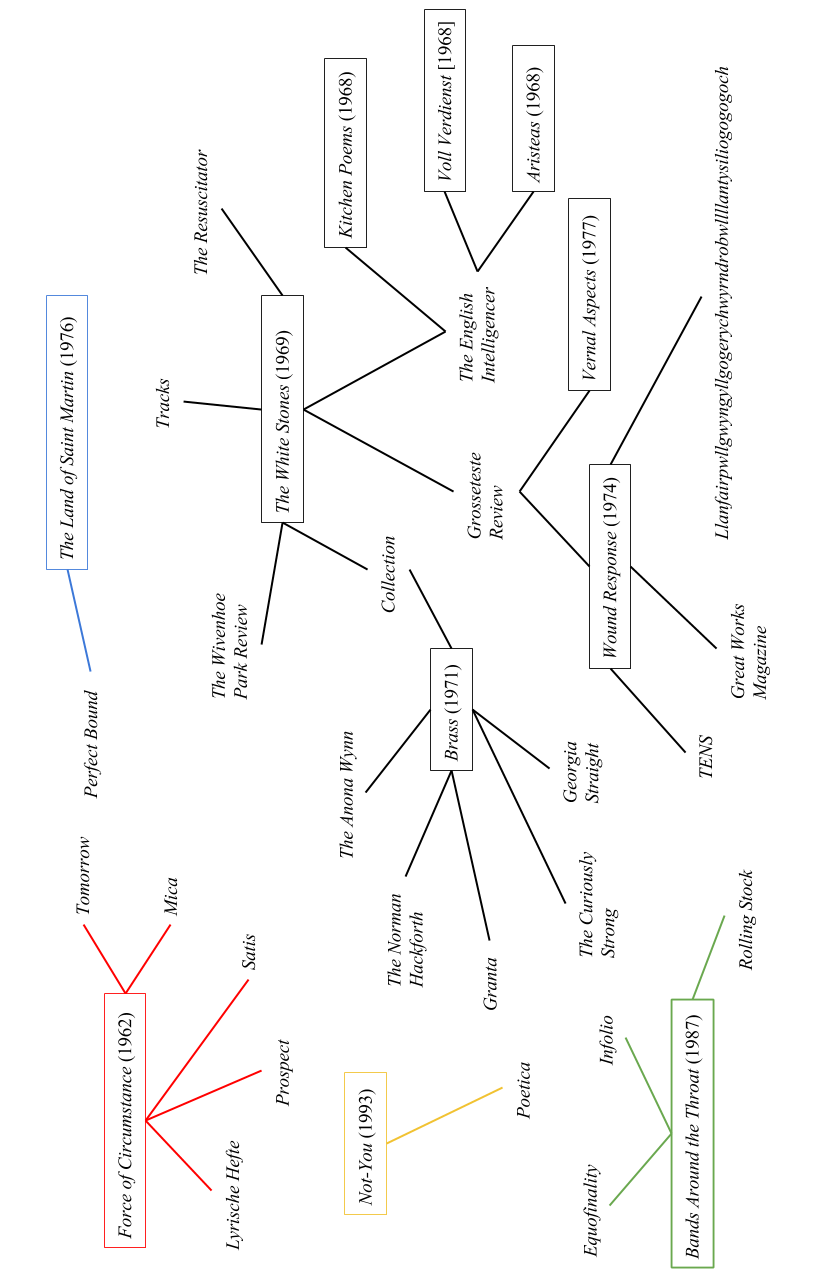
\includegraphics{figs/mags.png}
\caption{Prynne’s poetry collections, linked to the magazines in which
they were first published (in whole or in part)\label{fig:mags}}
\end{figure}

\newpage

\begin{figure}[htbp]
\centering
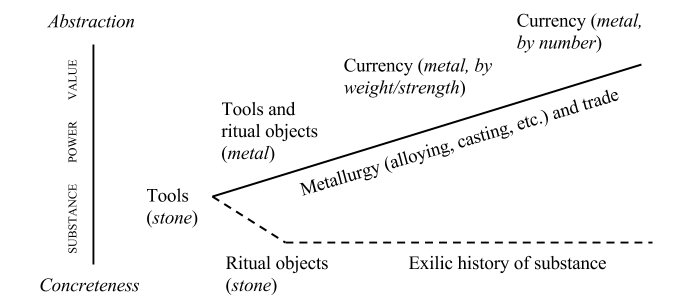
\includegraphics{figs/anm.png}
\caption{The argument of ‘A Note on Metal’\label{fig:anm}}
\end{figure}

\begin{figure}[htbp]
\centering
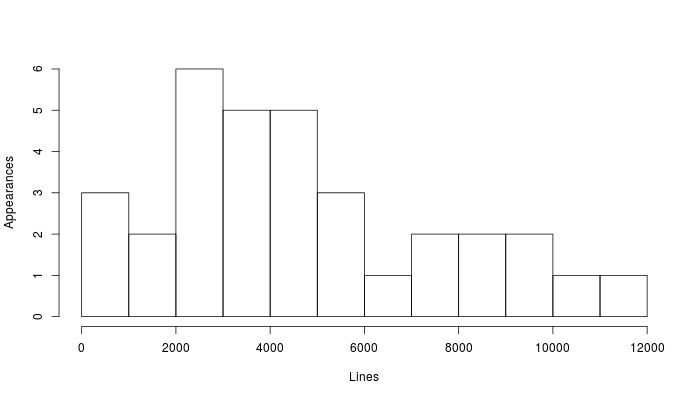
\includegraphics{figs/man.png}
\caption{Appearances of ‘man’ per 1,000 lines in \emph{Force of
Circumstance} (1962) and \emph{Poems} (2005)\label{fig:man}}
\end{figure}

\end{document}
